%------------------------------------------------------------
%	PREÁMBULO
%------------------------------------------------------------

\documentclass[A4, 11pt]{book} 

\usepackage{graphics,graphicx}
\usepackage{multicol}
\usepackage{multirow}
\usepackage{fancyhdr}
\usepackage{enumerate}
\usepackage[spanish,es-nodecimaldot,es-tabla]{babel}
\usepackage[utf8]{inputenc}
\usepackage[title]{appendix}
\usepackage{url}
\usepackage[hidelinks]{hyperref}
\usepackage{braket}
\usepackage{caption}
\usepackage{afterpage}
\usepackage{titling} 
\usepackage{float}
\usepackage{lscape}
\usepackage{selinput}
\usepackage{booktabs} 
\usepackage{lettrine}
\usepackage{color}
\usepackage{cancel}

\usepackage{amsfonts} 
\usepackage[centertags]{amsmath}
\usepackage{stmaryrd,amssymb,amsthm}
\usepackage{wasysym,mathrsfs}

\usepackage{xurl}

\usepackage[font=footnotesize,labelfont=small]{caption}
\captionsetup{width=0.85\linewidth}

\RequirePackage{geometry}
\geometry{margin=1.9cm}

\usepackage{parskip}
\setlength{\parskip}{0.2cm}
\setlength{\parindent}{0pt}

\usepackage[square,numbers,sort]{natbib}
\bibliographystyle{unsrt}

\usepackage{imakeidx}
\makeindex[columns=3, title=Índice Analítico, intoc]

% \selectlanguage{spanish}

% Bibliotecas para código
\usepackage{tcolorbox}
\usepackage{minted}


%------------------------------------------------------------
%	FORMATO DE PÁGINAS
%------------------------------------------------------------

\usepackage{fancyhdr}

\pagestyle{fancy}
\fancyhf{}

\renewcommand{\chaptermark}[1]{ \markboth{#1}{} }
\renewcommand{\sectionmark}[1]{ \markright{#1}{} }

\fancyhead[RO]{\leftmark \hspace{20pt} \thepage}
\fancyhead[LE]{\thepage \hspace{20pt} \rightmark}


%------------------------------------------------------------
%	DEFINICIONES
%------------------------------------------------------------


%------------------------------------------------------------
%	CARÁTULA
%------------------------------------------------------------

\title{Tesis}

\author{\textsc{Emmanuel Cruz Hernández}}

\date{}

\begin{document}

\raggedbottom

\thispagestyle{empty}

\begin{minipage}{.3\textwidth}
  \flushleft
  \center{
\includegraphics[scale=.09]{./Portada/unam.pdf}}

  \vspace{20pt}

  \center{
    \rule{.5pt}{.6\textheight}
    \hspace{7pt}
    \rule{2pt}{.6\textheight}
    \hspace{7pt}
    \rule{.5pt}{.6\textheight}
  } \\

  \center{
\includegraphics[scale=.22]{./Portada/ciencias.pdf}}
\end{minipage}
\begin{minipage}{.7\textwidth}
\flushright

\center{

  \center{
    \LARGE{U}\large{NIVERSIDAD} \LARGE{N}\large{ACIONAL} 
    \LARGE{A}\large{UTÓNOMA} \\[10pt]
    \large{DE} 
    \LARGE{M}\large{ÉXICO} 
  } \\
  \rule{\textwidth}{2pt}
  \\
  \hrulefill\\[1cm]
  
  \LARGE{F}\large{ACULTAD DE } \LARGE{C}\large{IENCIAS}\\[2cm]

  \large{ Skill de Alexa para apoyar el desarrollo de la Competencia de Manejo de Información }\\[2cm]

  \huge{
T \hspace{1cm} E \hspace{1cm} S \hspace{1cm} I \hspace{1cm} S  }\\[1cm]

  \large{QUE PARA OBTENER EL TÍTULO DE:}\\[1cm]

  \large{ Licenciado en Ciencias de la Computación }\\[1cm]

  \large{PRESENTA:}\\[1cm]

  \large{ Emmanuel Cruz Hernández }\\[1cm]

  \large{ Director de tesis  }\\[1cm]

  \large{ Dr. Gustavo De la Cruz Martínez }\\[1cm]

  \large{ Ciudad Universitaria, CD. MX. 2024. }
}

\end{minipage}



\thispagestyle{empty}

\newpage
\thispagestyle{empty}
\cleardoublepage


%------------------------------------------------------------
%	DEDICATORIA
%------------------------------------------------------------

\thispagestyle{empty}

\bigskip

\begin{flushright}

\vspace*{7cm}

	\textit{PENDIENTE}
	
	\textit{------}

\vspace*{\fill}

\end{flushright}

\newpage
\thispagestyle{empty}
\cleardoublepage
\addtocontents{toc}{\hfill \textbf{Página} \par}


%------------------------------------------------------------
%	AGRADECIMIENTOS
%------------------------------------------------------------

\chapter*{Agradecimientos}

PENDIENTE
\markboth{Agradecimientos}{Agradecimientos}
\addcontentsline{toc}{chapter}{Agradecimientos} 
\pagenumbering{roman}


%------------------------------------------------------------
%	ÍNDICE
%------------------------------------------------------------

\tableofcontents
\markboth{Índice general}{Índice general}
\pagenumbering{arabic}


%------------------------------------------------------------
%	CAPÍTULO I
%------------------------------------------------------------

%------------------------------------------------------------
%	CAPITULO I
%------------------------------------------------------------

\chapter{Introducción}
\label{capI}


%------------------------------------------------------------
%	INTRODUCCIÓN
%------------------------------------------------------------

Las interfaces de usuario basadas en voz (Voice User Interfaces) permiten que los usuarios interactúen con el sistema a través de la voz. Actualmente, los ejemplos más conocidos de este tipo de tecnología son los asistentes basados en voz (voice assistant) tales como Siri, Google Assistant y Alexa. La interacción basada en voz ofrece diferentes ventajas, entre ellas se pueden mencionar las siguientes: naturalidad y velocidad en la interacción, libertad de interacción sin uso de las manos y empatía.

En la educación los asistentes de voz ofrecen alternativas para personalizar el aprendizaje y el desarrollo de habilidades de los estudiantes. La introducción en la educación de esta tecnología ha crecido gracias a que las compañías que desarrollan estos asistentes, permiten la creación de aplicaciones y su uso sin costo.

Desde el punto de vista de la usabilidad, es un reto diseñar aplicaciones para estos asistentes, ya que deben permitir que los estudiantes sean capaces de utilizarlas sin la necesidad de la intervención de un profesor o tutor que los guíe para que puedan avanzar en el desarrollo de sus habilidades de forma autónoma.

Por otra parte, la pandemia derivada de la COVID-19 ha resaltado la necesidad de que los estudiantes desarrollen sus habilidades de búsqueda y organización de la información (information literacy), ya que los estudiantes tuvieron que recurrir a fuentes de información en línea y no siempre se revisaba que la información encontrada fuera válida, confiable y pertinente para resolver su problema de investigación. 

En este trabajo se explorará cómo se puede utilizar el asistente basado en voz Alexa para apoyar a los estudiantes a desarrollar sus habilidades de manejo de información, para ello se desarrollará una \textit{skill}\footnote{Las skills son aplicaciones desarrolladas para el servicio de Alexa} de Alexa, que les ayude a llevar a cabo una investigación siguiendo el Modelo Gavilán. El Modelo Gavilán es una estrategia que guía a los estudiantes a resolver problemas de búsqueda de información.

La skill será diseñada para estudiantes de México de entre 15 y 21 años. Para establecer los requerimientos de la aplicación, se analizará la información que reportaron los participantes de un diplomado dirigido a profesores de bachillerato y licenciatura de México y Chile, sobre los problemas que presentan los estudiantes al realizar una investigación, como lo son las técnicas basadas en copy-paste, omitir el análisis de contenido y autores.

El objetivo de este trabajo es diseñar una skill de Alexa, basada en el diseño centrado en el usuario para apoyar a los estudiantes a mejorar el proceso de investigación de información con una metodología formal de competencias de información conocida como el Modelo Gavilán.

La comprobación de la hipótesis central, tiene como objetivo apoyar a los estudiantes a desarrollar sus habilidades de manejo de información, a través de una skill para Alexa que les ayude a llevar a cabo una investigación siguiendo el Modelo Gavilán.

La organización de este trabajo es la siguiente: el Modelo Gavilán, el diseño de interfaces de usuario basadas en voz, el desarrollo de la skill y la conclusión. En el capítulo 2, Modelo Gavilán, se desarrollan y ejemplifican los objetivos de cada paso y subpaso que compone el proceso de búsqueda de información definido por la metodología para el desarrollo de la Competencia de Manejo de Información (CMI) conocida como el Modelo Gavilán.

En el capítulo 3, diseño de interfaces de usuario basadas en voz, se desarrollan los conceptos más importantes de las interfaces de usuario, así como las características de las interfaces multimodales, en particular las interfaces de usuario basadas en reconocimiento por voz. Así mismo, se desarrollan los conceptos relacionados a la metodología de diseño centrado en el usuario, técnicas y herramientas para el análisis del usuario y documentos para realizar evaluaciones de un sistema con usuarios.

En el capítulo 4, desarrollo de la skill, se introducen los conceptos de la configuración y creación de skills en la consola de desarrollo de Alexa, tales como invocaciones, intenciones, declaraciones, slots, entre otros. Durante el desarrollo de la skill se presenta también el análisis del problema, en el que se identifican las principales dificultades que presentan los alumnos de entre 15 y 21 años durante el proceso de búsqueda de información, con lo cual se realiza una análisis del usuario, con el fin de diseñar el funcionamiento de la skill basada en la metodología de diseño centrado en el usuario. Posteriormente se presenta el desarrollo de la implementación de la skill, en la que se describe cada parte que compone el sistema y las técnicas aplicadas, tales como el Custom Search JSON API y el Web Scraping. Al final del capítulo se desarrollan y analizan los resultados obtenidos de la evaluación de la skill con usuarios, usando el cuestionario de usabilidad llamado System Usability Scale (SUS).

Finalmente, en el último capítulo se expondrán las conclusiones finales del trabajo, así como las oportunidades de trabajo a futuro para desarrollar módulos que mejoren la usabilidad y experiencia de usuario de la skill.



%------------------------------------------------------------
%	CAPÍTULO II
%------------------------------------------------------------

%------------------------------------------------------------
%	CAPITULO I
%------------------------------------------------------------

\chapter{Modelo Gavilán}
\label{capII}


%------------------------------------------------------------
%	Competencia de Manejo de Información (CMI)
%------------------------------------------------------------

\section{Competencia de Manejo de Información (CMI)}
\label{secCMICap2}

La Internet es la red de comunicación más grande del mundo, en la que se transmiten millones de datos y se consultan grandes cantidades de información al día. A partir del gran crecimiento de información que se encuentra en la web, se vuelve complicado identificar información útil, relevante e importante para la investigación de algún tema particular, ya que existe gran variedad de autores y fuentes que tratan un mismo tema.

A partir de la dificultad de encontrar información en una red tan grande como la Internet, se desarrollaron algunas estrategias para realizar investigaciones de mayor calidad, enfocada principalmente a estudiantes.

% REFERENCIA
López (2007) señala que la competencia de manejo de información (CMI) es un conjunto de habilidades, conocimientos y actitudes que el estudiante necesita para poder identificar puntualmente qué es lo que requiere saber sobre un tema, buscar la información de la mejor forma, señalar si la información responde a sus necesidades y convertirla en conocimiento útil para aplicarla en diferentes contextos.

La CMI fomenta y desarrolla las habilidades necesarias para obtener la capacidad de formular preguntas específicas que concreten la información que se requiere obtener, la elaboración de una estrategia que permita sintetizar y analizar la información de las preguntas formuladas, identificar y encontrar las fuentes más útiles y confiables, encontrar en su contenido la información buscada, evaluar la calidad la información tomando como base las necesidades a resolver en la investigación, clasificar la información para facilitar la síntesis, analizar y sintetizar la información en un formato útil y claro.

% REFERENCIA
De acuerdo con López (2007), una competencia es la combinación de dos factores importantes que son las capacidades y las actitudes (ver Figura \ref{fig:21}). Por un lado, la capacidad se compone de conocimientos y habilidades, que es todo aquello que se sabe y se conoce junto con todo aquello de lo que se puede hacer de forma correcta. Por otro lado, la actitud se refiere a las disposiciones. Es decir, que para poder lograr una competencia, se debe contar con la capacidad, que involucra saber, conocer, hacer, y también se debe contar con actitud, la buena disposición a lograr un objetivo.

\begin{figure}[H]
% \begin{figure}
  \centering
  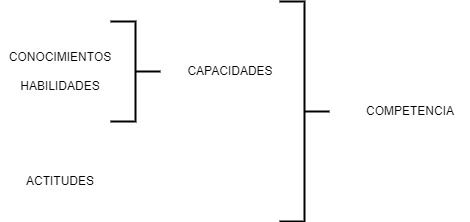
\includegraphics[width=0.70\textwidth]{Cap2/Figuras/CMI.jpg}
  \caption{Elementos constitutivos de capacidades y competencia. López (2007)}
  \label{fig:21}
\end{figure}

La abrumadora cantidad de información en la web y el desarrollo de la competencia de manejo de información, dio paso a la creación de metodologías que orientan el proceso de investigación de información. A estas se le conocen como metodologías para el desarrollo de la CMI.

%------------------------------------------------------------
%	Metodologías para el desarrollo de la CMI
%------------------------------------------------------------

\section{Metodologías para el desarrollo de la CMI}
\label{secMetodologiasCap2}

El proceso para desarrollar las habilidades de identificar y analizar las decisiones involucradas en la búsqueda de información, requiere de un proceso en el que se definen los pasos a seguir para adquirir buenos hábitos de investigación y convertirlos en una habilidad en la práctica.

A partir de la necesidad de contar con un mecanismo o una estrategia para adquirir las habilidades involucradas en la CMI, nacen diferentes metodologías que impulsan el desarrollo de la CMI. 

Estas metodologías consideran las propiedades base de la CMI, tales como realizar un proceso de búsqueda, análisis, organización y síntesis de la información encontrada en fuentes como libros, blog, páginas web, revistas, entre otros. Por otro lado, las metodologías también deben promover que los estudiantes utilicen  los conocimientos adquiridos.

% REFERENCIAS
Actualmente, existen diferentes metodologías que definen un conjunto de pasos para desarrollar la CMI. González y Sánchez (2007) señalan que algunas de las metodologías existentes son las siguientes:

\begin{itemize}
  \item La metodología de la Asociación de Bibliotecas Escolares de Ontario, Canadá.
  \item La metodología \textit{Big 6}, creada por Eisenberg y Berkowitz.
  \item La metodología \textit{Ciclo de Investigación} creada por Jaime Mckenzie.
  \item La metodología \textit{Modelo de Proceso para Búsqueda de Información (ISP)}, creada por Carol Kuhlthau.
  \item El \textit{Modelo de Irving para Competencias para el Manejo de la Información}, creado en Reino Unido.
  \item El \textit{Modelo de Stripling y Pitts del Proceso de Investigación}, creado en Estados Unidos.
  \item El \textit{Modelo Gavilán}, de la Fundación Gabriel Piedrahita Uribe, creada en Colombia.
\end{itemize}

Cada una de las metodologías tiene un comportamiento diferente pero todas pretenden lograr el mismo objetivo, desarrollar la CMI.
 
La mayor parte de estos modelos dividen su estrategia de búsqueda de información de entre cuatro pasos a 16 pasos, los cuales se agrupan en 4 etapas principales: búsqueda de fuentes, análisis y evaluación, interpretación, y síntesis de la información.

%------------------------------------------------------------
%	Pasos del Modelo Gavilán
%------------------------------------------------------------

\section{Pasos del Modelo Gavilán}
\label{secPasosCap2}

% REFERENCIA
González y Sánchez (2007) señalan que el Modelo Gavilán es un modelo que surge en Colombia por la Fundación Gabriel Piedrahita Uribe. Este modelo fue dividido en cuatro etapas que conforman el proceso de investigación de información, basado en los objetivos de la CMI.

Los cuatro pasos que conforman el Modelo Gavilán son: 1) definir el problema de investigación, 2) buscar y evaluar información, 3) análisis de la información y 4) sintetizar la información. Estos pasos se siguen como en la Figura \ref{fig:22}.

\begin{figure}[H]
% \begin{figure}
  \centering
  \includegraphics[width=0.70\textwidth]{Cap2/Figuras/Modelo Gavilán.jpg}
  \caption{Pasos fundamentales del Modelo Gavilán. González y Sánchez (2007)}
  \label{fig:22}
\end{figure}

A su vez, cada paso definido en el Modelo Gavilán, contiene una serie de subpasos, en los que se divide específicamente la acción que se debe realizar al momento de realizar una investigación.

%------------------------------------------------------------
%	Definición del problema de investigación
%------------------------------------------------------------

\subsection{Definición del problema de investigación}
\label{secPaso1Cap2}

La etapa de definición del problema de la investigación tiene como objetivo desarrollar las habilidades necesarias para delimitar la búsqueda de información de un tema, así como desarrollar estrategias para plantear un problema de información y establecer un límite para conocer con cierta exactitud el rubro del tema que se quiere conocer.

Para lograrlo, es importante definir la necesidad de información en un contexto o situación determinada, que enfoque el comienzo de la investigación en forma de una \textit{pregunta inicial}. Una vez definido qué es lo que se necesita investigar, se recurre a la identificación de temas centrales que abarquen la información que sea útil a la investigación, tales como conceptos, definiciones y descripciones relevantes del tema en el que se centra la información.

Los aspectos anteriores a desarrollar se dividen en subpasos que conforman el primer paso del Modelo Gavilán. Este se compone de los siguientes subpasos:

\begin{itemize}
  \item [1a.] Plantear una pregunta inicial
  \item [1b.] Analizar la pregunta inicial
  \item [1c.] Construir un plan de investigación
  \item [1d.] Formular preguntas secundarias
  \item [1e.] Evaluar el paso 1
\end{itemize}

Estos subpasos se siguen como en la Figura \ref{fig:23}.

\begin{figure}[H]
% \begin{figure}
  \centering
  \includegraphics[width=0.70\textwidth]{Cap2/Figuras/Definición del problema.jpg}
  \caption{Definición del problema de investigación. González (2007)}
  \label{fig:23}
\end{figure}

%------------------------------------------------------------
%	Subpaso 1a: Plantear una pregunta inicial
%------------------------------------------------------------

\subsubsection{Subpaso 1a: Plantear una pregunta inicial}
\label{secPaso1aCap2}

El objetivo de este subpaso es que los estudiantes adquieran la habilidad de iniciar una investigación, a partir de la formulación de preguntas iniciales para plantear problemas de información. Con este subpaso, se busca que el estudiante comprenda la utilidad de comenzar la exploración de un tema, con base en preguntas para delimitar un tema nuevo que probablemente es desconocido para el estudiante. Asimismo, se tiene como objetivo identificar una pregunta inicial adecuada, que es aquella que mejor delimita el tema de la investigación.

Es importante mencionar que no todas las preguntas generadas de un tema son preguntas iniciales. Las preguntas iniciales adecuadas abarcan diferentes conceptos, características, subtemas o aspectos de un tema. Es decir, son preguntas cuya respuesta no es concreta, como la fecha de un acontecimiento histórico, el lugar de nacimiento de algún personaje, etc. Por el contrario, las preguntas iniciales son preguntas que pueden abarcar toda esta información de un tema, en donde está involucrada información que responde a las preguntas cómo, cuándo, dónde, etc. Este tipo de preguntas da la posibilidad a los estudiantes de realizar una tarea de reflexión sobre el tema de investigación, para dar contexto e identificar la importancia de obtener información diversa de un tema delimitado.

% REFERENCIA
González (2007) señala que una pregunta inicial surge a partir de un problema de información, y para que pueda formularse de forma adecuada, se deben cumplir dos características importantes que se presentan a continuación:

\begin{enumerate}
  \item Requerir información ya existente, que esté disponible en fuentes de información como páginas web, libros, revistas, enciclopedias, etc.
  \item Plantearse a partir de un contexto o situación real que despierte la curiosidad del estudiante, para analizar y aplicar los conocimientos que se adquieren durante la investigación.
\end{enumerate}

Por ejemplo, si un alumno quiere saber sobre matemáticas, se vuelve complejo investigar el tema de forma general, ya que la información que se puede encontrar sobre el tema es muy extensa. Sobre matemáticas podrían surgir preguntas como ¿qué son las matemáticas?, ¿qué es la álgebra?, ¿cómo se resuelven las derivadas?, ¿cómo se demuestra un teorema matemático?, e incluso preguntas como ¿las matemáticas se inventaron o se descubrieron? o ¿crees que eres malo para las matemáticas?

Para este ejemplo tomaremos como pregunta inicial la última propuesta, ¿crees que eres malo para las matemáticas?, la cual cumple con las dos características para formular una pregunta inicial adecuada mencionadas anteriormente. La respuesta a esta pregunta requiere de información que ya existe en diferentes fuentes de información, además de plantear si los conocimientos de esta pregunta pueden adaptarse a un contexto real.

%------------------------------------------------------------
%	Subpaso 1b: Analizar la pregunta inicial
%------------------------------------------------------------

\subsubsection{Subpaso 1b: Analizar la pregunta inicial}
\label{secPaso1bCap2}

Este subpaso consiste en desarrollar habilidades para examinar con detalle el límite de la pregunta inicial propuesta. En esta etapa se distinguen los distintos subtemas que pueden estar  englobados en la pregunta inicial, con el fin tener conocimiento sobre la información involucrada en la investigación. A su vez, se determina si el enfoque de la pregunta inicial es correcto de acuerdo con los propósitos de la investigación, es decir, que ésta pueda incluir todos aquellos puntos que son necesarios considerar y conocer como resultado de la investigación.

El análisis de una pregunta inicial permite crear un límite en la profundidad de la investigación de un tema y dar dirección al estudiante en forma de guía para delimitar un tema amplio, en detalles específicos, ya que por lo general, no es necesario conocer absolutamente todo el tema y los subtemas que se puedan derivar del mismo, sino que sólo es necesario incluir ciertos detalles en el proceso de investigación.

Los aspectos específicos de un tema, involucrados en la pregunta inicial, pueden considerarse como categorías, jerarquías o clases, dependiendo del contexto del tema, de tal manera que se forma una clasificación del contenido. Una estrategia para identificar esta clasificación de información, es manifestar, en forma oral o escrita, todo lo que se sabe sobre el tema de investigación en forma de hipótesis, que no necesariamente son verdaderas, tomando en cuenta aspectos que van desde lo más general hasta lo más particular y con ello tratar de responder a la pregunta inicial. El hecho de responder o dar una respuesta aproximada a la pregunta inicial aporta una pauta importante para identificar las clases, jerarquías o categorías del conocimiento que se quiere saber al final de la investigación.

Una segunda estrategia consiste en buscar información en Internet, libros, revistas o cualquier fuente de información, de forma rápida y no exhaustiva, es decir, una breve búsqueda sobre el tema sin involucrar detalles específicos, con el fin de generar una idea, de forma general, sobre el tema. Esta búsqueda permite producir ideas y conocimiento sobre aspectos sobresalientes del tema, que pueden representarse como posibles categorías. Con ello, se permite identificar aquellos temas que necesitan mayor profundidad y dar dirección a la información útil para responder la pregunta inicial.

Cabe mencionar que las dos estrategias anteriores son un apoyo para poder identificar las categorías y valorar sí la pregunta inicial es la más adecuada para comenzar la investigación. Ambas estrategias pueden usarse individualmente o como complemento una de la otra, para desarrollar de mejor manera el análisis de la pregunta inicial. En caso de que la pregunta inicial no contenga información útil para el conocimiento de la investigación final, será necesario considerar otra pregunta como pregunta inicial o reestructurar la formulación de la pregunta.

Retomando el ejemplo de la pregunta inicial seleccionada, ¿crees que eres malo para las matemáticas?, se presentan a continuación algunas hipótesis correspondientes a la primera estrategia e información de fuentes de información correspondientes a la segunda estrategia.

\begin{table}[H]
  \begin{center}
    \begin{tabular}{ | p{8cm} | p{8cm} | }
      \hline
      HIPÓTESIS (PRIMERA ESTRATEGIA) & FUENTES DE INFORMACIÓN (SEGUNDA ESTRATEGIA) \\ \hline
      \begin{itemize}
        \item Si me cuesta trabajo realizar cuentas, soy malo para las matemáticas.
        \item Si las matemáticas no son de mi interés, entonces soy malo en matemáticas.
        \item Si cualquier materia de matemáticas me aburre, entonces soy malo para matemáticas.
        \item Si no estudio alguna ingeniería, entonces no soy bueno en matemáticas.
        \item Si soy filósofo, entonces soy malo para las matemáticas.
      \end{itemize} & 
      \begin{itemize}
        \item Ruef (2020) señala que $"$El 'trauma matemático' se manifiesta como ansiedad o temor, un miedo debilitante a equivocarse.$"$
        \item Ruef (2020) señala que $"$los estudiantes que tienen éxito en las pruebas de datos matemáticos cronometrados, pueden creer que ser buenos en matemáticas$"$
        \item Sautoy (2015) señala que $"$muchos expertos advierten que el hablar de 'genes matemáticos' es una falacia, pues lo que se requiere para ser bueno en matemáticas es esforzarse$"$
      \end{itemize} \\ \hline
    \end{tabular}
    \caption{Ejemplo de estrategias del subpaso 1a del Modelo Gavilán.}
    \label{tab:t1}
  \end{center}
\end{table}

De la información presentada en la Tabla \ref{tab:t1}, podemos identificar aspectos para clasificar la información útil y necesaria para considerar en la investigación. Algunos aspectos de ellos pueden ser los siguientes:

\begin{itemize}
  \item Definición de trauma matemático.
  \item Aspectos a considerar para aprender matemáticas.
  \item Definición de genes matemáticos.
  \item Relación entre el trauma matemático y el desinterés o aburrimiento por las matemáticas.
  \item Escritores que son matemáticos.
\end{itemize}

%------------------------------------------------------------
%	Subpaso 1c: Construir un plan de investigación
%------------------------------------------------------------

\subsubsection{Subpaso 1c: Construir un plan de investigación}
\label{secPaso1cCap2}

Este paso consiste en desarrollar las habilidades para definir la organización y el orden en que se realizará la investigación. Una vez identificada una pregunta inicial adecuada, así como las distintas categorías que abarca, se planea el orden en que se comenzará a investigar cada una de las categorías, con el fin de dar el seguimiento más adecuado a la investigación en orden cronológico, jerárquico o por profundidad del tema.

La planeación de la forma de investigación permite obtener una guía durante el proceso de investigación, del cual se produce un objetivo más claro sobre la información que es adecuada y útil para la investigación final. En esta etapa también se considera un filtro de categorías que no aportan información relevante a la investigación, así como la identificación de las categorías que sí aportan información útil, para poder ordenarlas y dar seguimiento al orden en que se va a examinar cada una de las categorías identificadas en el subpaso 1b.

% REFERENCIA
González (2007), señala que una estrategia que se puede seguir para poder realizar un plan de investigación adecuado incluye los siguientes pasos:

\begin{itemize}
  \item Identificar las categorías que son más adecuadas para responder a la pregunta inicial. Por otra parte, omitir aquellas categorías que no aportan información útil para responder a la pregunta inicial, estas las podemos denominar como categorías secundarias.
  \item Determinar y decidir si las categorías encontradas en el paso anterior son suficientes para poder responder la pregunta inicial. En caso de que falten puntos por cubrir para responder la pregunta inicial, es necesario identificar cuales son las categorías faltantes y agregarlas a las categorías actuales.
  \item Establecer el orden más adecuado para dar seguimiento a la investigación. El orden puede ser cronológico, por jerarquía, por profundidad, etc. Con ello se facilita la comprensión de la información para el mejor entendimiento del tema.
  \item Por cada una de las categorías ya ordenadas, identificar cuáles son los aspectos que son necesarios conocer y que aporten utilidad a la información final de la investigación.
\end{itemize}

Retomando el ejemplo anterior y las categorías antes identificadas. Siguiendo la estrategia mencionada anteriormente, el primer paso señala que es importante determinar cuáles categorías son importantes y desechar aquellas que no aportan contenido útil a la respuesta de la pregunta inicial. En este caso, no sería necesario conocer la definición de genes matemáticos, la relación entre el trauma matemático y el desinterés, así como saber información de filósofos que han sido matemáticos. Por lo que la lista se reduce como sigue:

\begin{itemize}
  \item Definición de trauma matemático.
  \item Aspectos a considerar para aprender matemáticas.
\end{itemize}

El segundo paso propone realizar un análisis para saber si las categorías son suficientes para responder a la pregunta inicial. En este caso, también puede ser de interés las causas del trauma matemático. Esta nueva categoría que se agrega queda como sigue.

\begin{itemize}
  \item Definición de trauma matemático.
  \item Aspectos a considerar para aprender matemáticas.
  \item Causas del trauma matemático.
\end{itemize}

El tercer punto menciona que es útil establecer un orden entre las categorías. En este caso, no es tan claro investigar las causas del trauma matemático sin antes saber qué es el trauma matemático, por lo que se debe investigar antes. Los aspectos a considerar para aprender y fortalecer la habilidad matemática se derivan de las causas, por lo que esta se puede investigar después. Estas observaciones modifican el orden de la lista de categorías como sigue.

\begin{itemize}
  \item Definición de trauma matemático.
  \item Causas del trauma matemático.
  \item Aspectos a considerar para aprender matemáticas.
\end{itemize}

Finalmente, se identifican aspectos específicos, en caso de haberlos, por cada una de las categorías:

\begin{itemize}
  \item Definición de trauma matemático.
    \begin{itemize}
      \item Quién define el concepto.
      \item Cuándo surge.
    \end{itemize}
  \item Causas del trauma matemático.
    \begin{itemize}
      \item A quiénes afecta.
      \item Cómo se manifiesta el trauma matemático.
    \end{itemize}
  \item Aspectos a considerar para aprender matemáticas.
    \begin{itemize}
      \item Tipo de ejercicios a considerar.
      \item Estrategias de práctica.
    \end{itemize}
\end{itemize}

%------------------------------------------------------------
%	Subpaso 1d: Formular preguntas secundarias
%------------------------------------------------------------

\subsubsection{Subpaso 1d: Formular preguntas secundarias}
\label{secPaso1dCap2}

Este paso consiste en identificar aquellos aspectos específicos de cada categoría que aporten información útil a la investigación final a partir de preguntas secundarias. Estas preguntas tienen el propósito de brindar información de aspectos específicos que son importantes mencionar en la investigación según lo propuesto en la construcción del plan de investigación.

Las preguntas secundarias tienen la característica de ser más concretas y apuntar a información más específica, ya que da respuesta a detalles precisos de algún tema, lo cual determina el contenido que apoya a responder la pregunta inicial en conjunto.

Para poder crear las preguntas secundarias, es necesario tomar los aspectos que son necesarios conocer en la investigación, mismos que fueron identificados en el paso 1c. Una vez que se tiene el conjunto de aspectos a conocer, se procede a convertir cada característica específica en una pregunta, de tal forma que la pregunta pueda darle una respuesta concreta, sin perder de vista que estas preguntas no deben ser muy sencillas ni muy complejas.

Tanto el plan de investigación como la creación de preguntas secundarias, puede ir creciendo conforme avanza la investigación, con el fin de retroalimentar la información con detalles faltantes o a forma de complemento, sin embargo, es recomendable que los aspectos importantes de la investigación, así como las preguntas secundarias, queden bien definidas durante la primera etapa de definición del problema, para que no exista confusión durante los siguientes pasos del Modelo Gavilán.

Para este ejemplo, se obtuvo la lista de categorías, aspectos a considerar y su pregunta secundaria asociada, como se muestra en la Tabla \ref{tab:t2}.

\begin{table}[H]
  \begin{center}
    \begin{tabular}{ | p{8cm} | p{8cm} | }
      \hline
      CATEGORÍAS Y ASPECTOS A CONSIDERAR & PREGUNTA SECUNDARIA ASOCIADA A LOS ASPECTOS \\ \hline
      Definición de trauma matemático
      \begin{itemize}
        \item Quien define el concepto.
        \item Cuándo surge.
      \end{itemize} & 
      \begin{itemize}
        \item ¿Qué es el trauma matemático?
        \item ¿Quien definió el significado de trauma matemático?
        \item ¿Cuándo se definió el trauma matemático?
      \end{itemize} \\ \hline

      Causas del trauma matemático
      \begin{itemize}
        \item A quienes afecta.
        \item Cómo se manifiesta el trauma matemático.
      \end{itemize} & 
      \begin{itemize}
        \item ¿Quienes pueden ser afectados por el trauma matemático?
        \item ¿Cómo puede presentarse el trauma matemático?
      \end{itemize} \\ \hline

      Aspectos a considerar para aprender matemáticas
      \begin{itemize}
        \item Tipo de ejercicios a considerar.
        \item Estrategias de práctica.
      \end{itemize} & 
      \begin{itemize}
        \item ¿Qué tipo de ejercicios se pueden realizar para mejorar en matemáticas?
        \item ¿Qué estrategias se pueden seguir para practicar ejercicios matemáticos?
      \end{itemize} \\ \hline
    \end{tabular}
    \caption{Ejemplo de preguntas secundarias del paso 1d del Modelo Gavilán.}
    \label{tab:t2}
  \end{center}
\end{table}

%------------------------------------------------------------
%	Subpaso 1e: Evaluación del paso 1
%------------------------------------------------------------

\subsubsection{Subpaso 1e: Evaluación del paso 1}
\label{secPaso1eCap2}

El objetivo principal del primer paso del Modelo Gavilán es obtener las habilidades para identificar, analizar y delimitar la información relacionada con un tema muy general, por lo que la evaluación del primer paso consiste en evaluar los criterios definidos para calificar las habilidades de identificación y delimitación de información, así como las habilidades para comprender el inicio de búsqueda de información de un tema a partir de la creación de una guía.

Para poder evaluar de mejor manera si se adquirieron las habilidades de búsqueda de información, se puede diseñar una lista de preguntas que califiquen las tareas realizadas en cada paso. Algún tutor a cargo de la tarea de investigación de los estudiantes, puede determinar si los subpasos se cumplieron.

% REFERENCIA
El equipo de EDUTEKA desarrolló algunas preguntas para el apoyo de la evaluación del primer paso del Modelo Gavilán, llamado LISTA DE VERIFICACIÓN - EVALUACIÓN DEL PASO 1 (MODELO GAVILÁN), que puede consultarse en EDUTEKA (2007).

%------------------------------------------------------------
%	Búsqueda y evaluación de fuentes de información
%------------------------------------------------------------

\subsection{Búsqueda y evaluación de fuentes de información}
\label{secPaso2Cap2}

Este paso consiste en desarrollar las habilidades para indagar en las fuentes de información, con el fin de encontrar contenido útil para resolver el problema de información. A su vez, se desarrollan estrategias para determinar si las fuentes de información son útiles para cubrir las necesidades de la investigación, así como decidir si la información es confiable y de buena calidad.

Para lograr los objetivos de este paso, es necesario conocer las fuentes de información disponibles, así como sus características y formas de uso, con el fin de identificar cuáles fuentes de información proporcionan más conocimiento útil y aportan un mejor resultado en el contenido de la investigación.

Las habilidades propuestas, se detallan en cuatro subpasos que conforman la búsqueda y evaluación de fuentes de información. Estos subpasos son:

\begin{itemize}
  \item [2a.] Identificar y seleccionar las fuentes de información más adecuadas
  \item [2b.] Acceder a las fuentes de información seleccionadas
  \item [2c.] Evaluar las fuentes de información encontradas
  \item [2d.] Evaluación del paso 2
\end{itemize}

Estos subpasos se siguen como en la Figura \ref{fig:24}.

\begin{figure}[H]
% \begin{figure}
  \centering
  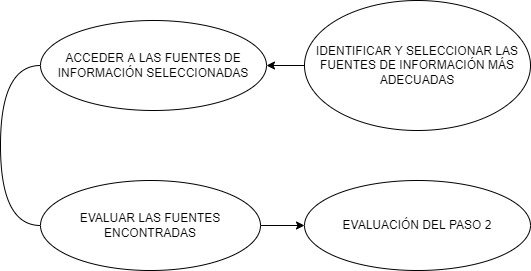
\includegraphics[width=0.70\textwidth]{Cap2/Figuras/Búsqueda y evaluación de información.jpg}
  \caption{Búsqueda y evaluación de fuentes de información. González (2007)}
  \label{fig:24}
\end{figure}

%------------------------------------------------------------
%	Subpaso 2a: Identificar y seleccionar las fuentes de información más adecuadas
%------------------------------------------------------------

\subsubsection{Subpaso 2a: Identificar y seleccionar las fuentes de información más adecuadas}
\label{secPaso2aCap2}

El objetivo de este subpaso es desarrollar la habilidad de reconocer las fuentes de información más adecuadas para la investigación, es decir, los recursos utilizados para extraer información. Existen diferentes fuentes de información, por lo que es importante la identificación de las fuentes de información que son de mayor utilidad para el proceso de investigación, dependiendo de las necesidades identificadas en el análisis de la definición y del problema de investigación.

Algunas fuentes de información más utilizadas son libros, blogs, páginas de internet, revistas, periódicos, videos, podcast, entre otros. Cada una de ellas cuenta con características que pueden aportar mayor o menor utilidad a la investigación, dependiendo del tema y la organización planeada en el paso de definición y planeación.

% REFERENCIA
Polo (2022) señala que existen tres diferentes tipos de fuentes de información:

\begin{itemize}
  \item \textbf{Fuentes primarias.} Las fuentes de información primarias son aquellas que son publicadas directamente por su autor por primera vez, y por tanto, es información que no ha sido filtrada, interpretada o evaluada previamente por un tercero. Tales como libros, notas de revista, notas periodísticas, reportes de investigación, fotografías, videos u obras de arte originales.Las fuentes de información primarias son aquellas que son publicadas directamente por su autor por primera vez, y por tanto, es información que no ha sido filtrada, interpretada o evaluada previamente por un tercero. Tales como libros, notas de revista, notas periodísticas, reportes de investigación, fotografías, videos u obras de arte originales.
  \item \textbf{Fuentes secundarias.} Las fuentes secundarias ofrecen información que ya ha sido procesada a partir de fuentes primarias en un orden específico. Es decir, proporciona información que aplica cierto criterio para dar a conocer información específica, tales como resúmenes, catálogos, diccionarios, enciclopedias, fuentes biográficas, bibliografías, atlas, manuales, entre otras.
  \item \textbf{Fuentes terciarias.} Estas fuentes funcionan como apoyo o guía, para encontrar información en fuentes primarias y secundarias. Tales como un índice de artículos generales de publicaciones de periódico, el catálogo de una biblioteca, una bibliografía, o el motor de búsqueda de un navegador web.
\end{itemize}

Entender las diferencias entre fuentes de información y sus características, aportan una habilidad para reconocer cuáles son las más adecuadas para la investigación, dependiendo del tema que se necesita investigar. Además, dominar la selección de tipos de fuentes de información, ayuda al estudiante a saber qué tan alejada está la información de hechos fidedignos, logrando con ello, conseguir información de mayor calidad, confiable y con mayores aportaciones al contenido de la investigación.

% REFERENCIA
Existen diferentes tipos de información que son importantes conocer, para enfocar de mejor forma las fuentes de información a utilizar. Burkhardt, MacDonald y Rathemacher (2003) señalan que existen cuatro tipos de información presentados a continuación:

\begin{itemize}
  \item \textbf{Información factual.} Es aquella información que tiene forma de comprobarse y que está basada en hechos. Este tipo de información no cambia y en todas las fuentes de información que se consulte, esta tiene exactamente los mismos datos. Tal es el caso de teorías físicas, matemáticas, métodos científicos probados, etc.
  \item \textbf{Información analítica.} Este tipo de información es el resultado de la interpretación y el análisis de la información factual. Es decir, es información resultante de la investigación de expertos en un tema y que por lo general se publica en libros o notas periodísticas. Esta información implica un proceso o reflexión de cómo se llegan a los resultados propuestos en la conclusión de la información.
  \item \textbf{Información subjetiva.} Esta información es resultado de la opinión y el punto de vista de un grupo o de un individuo sobre algún tema. Es información que contiene la perspectiva del autor o autores, sin ser necesariamente información fidedigna.
  \item \textbf{Información objetiva.} Es información que contiene la simplificación de un tema, del cuál se toman diferentes fuentes de información para crear una síntesis de aspectos relevantes para un enfoque específico. Este tipo de información puede tener en su contenido una combinación de los diferentes tipos de información anteriores. Sin embargo, a diferencia de la información subjetiva, esta no incluye posturas de los autores.
\end{itemize}

La identificación de fuentes de información, así como el tipo de información que se requiere buscar para la investigación, son aspectos fundamentales que facilitan la búsqueda y la evaluación de fuentes, tomando en cuenta el origen de la información. A pesar de que varias de las fuentes de información pueden encontrarse en formato digital, es importante mencionar que cada fuente tiene características individuales que pueden sobresalir para realizar una mejor investigación de un tema específico.

Retomando el ejemplo, ¿crees que eres malo para las matemáticas?, la información relacionada con la pregunta puede surgir de un estudio psicológico o algún artículo matemático. Las fuentes de información más adecuadas para encontrar esta información pueden basarse en un estudio cognitivo o estadístico, sin importar si está publicado en internet o en un libro.

%------------------------------------------------------------
%	Subpaso 2b: Acceder a las fuentes de información seleccionadas
%------------------------------------------------------------

\subsubsection{Subpaso 2b: Acceder a las fuentes de información seleccionadas}
\label{secPaso2bCap2}

En este subpaso se utilizan diferentes estrategias para explorar las distintas fuentes de información de forma correcta.

Dependiendo del tipo de fuente de información, la forma en que se accede a esta varía. Cada fuente de información cuenta con una estrategia de búsqueda distinta, un índice para los libros, categorías o secciones para los periódicos, clases o motores de búsqueda para fuentes en la Internet, catálogos y códigos para una biblioteca, entre otros.

Es importante utilizar palabras clave en esta etapa para facilitar la búsqueda. Las palabras clave son términos sobresalientes del tema a investigar, que limita y facilita la búsqueda de la información. Es útil identificar estas palabras para realizar una búsqueda más rápida y precisa en las diferentes fuentes de información.

Además de identificar palabras clave, es primordial determinar cuáles son los aspectos involucrados en la búsqueda, con el fin de formular una frase que limite el tema dentro de la fuente de información. Es decir, se determinan aspectos como fechas, hechos importantes, teorías, personajes históricos, etc., para formar una frase a partir del aspecto a conocer y las palabras clave identificadas.

Una estrategia para poder formular estas frases, es tomar información del conjunto de preguntas secundarias de las cuales se pueden extraer aspectos específicos por conocer. Las palabras clave, en cambio, pueden obtenerse tanto de las preguntas secundarias como de la pregunta inicial, definida en el primer paso del Modelo Gavilán.

En esta etapa se consigue la ubicación de la información que puede ser relevante para la investigación o que puede contener datos que son indispensables para responder las preguntas secundarias. Todos estos resultados se almacenan en una bitácora para poder consultarlo posteriormente. Dependiendo del tipo de fuente de información, la bitácora debe almacenar información específica, como la URL para las páginas web, el número de la página de un libro, el artículo de una revista, la página de una enciclopedia, etc.

Cabe mencionar que es posible tener más de una fuente de información para cada una de las frases propuestas para la búsqueda. Puede ser una combinación de fuentes de información o una misma fuente de información de diferente autor.

Por ejemplo, algunas frases para encontrar información útil para la investigación, considerado la pregunta inicial y las preguntas secundarias son las siguientes:

\begin{itemize}
  \item Significado del trauma matemático.
  \item Autor del trauma matemático.
  \item Causas del trauma matemático.
  \item Solución al trauma matemático.
\end{itemize}

Las frases anteriores, son un apoyo para poder encontrar información de forma más relevante para la investigación. Los resultados de la búsqueda se pueden almacenar en una bitácora como en la Tabla \ref{tab:t3}.

\begin{table}[H]
  \begin{center}
    \begin{tabular}{ | p{2cm} | p{6cm} | p{2cm} | p{6cm} | }
      \hline
      No. DE FUENTE & INFORMACIÓN & FUENTE DE INFORMACIÓN & UBICACIÓN DE LA INFORMACIÓN \\ \hline
      1 & 
      \begin{itemize}
        \item Significado del trauma matemático
        \item Autor del trauma matemático
        \item Causas del trauma matemático
      \end{itemize} & Internet & \url{https://theconversation.com/crees-que-eres-malo-para-las-matematicas-puedes-sufrir-un-trauma-matematico-143507#:~:text=El%20'trauma%20matem%C3%A1tico'%20se%20manifiesta,las%20opciones%20escolares%20y%20 profesionales}
       \\ \hline

      2 & 
      \begin{itemize}
        \item Causas del trauma matemático
      \end{itemize} & Artículo digital & Novelo, S., Herrera, S., Díaz, J., Salinas, H. (2025), Temor a las matemáticas: causa y efecto
       \\ \hline
      
      3 & 
      \begin{itemize}
        \item Causas del trauma matemático
      \end{itemize} & Internet & \url{https://www.trahtemberg.com/articulos/3472-el-trauma-matematico.html}
       \\ \hline
      
      4 & 
      \begin{itemize}
        \item Solución al trauma matemático
      \end{itemize} & Internet & \url{https://harmonia.la/mente-y-emociones/salud-mental/te-consideras-malo-para-las-matematicas-quiza-sufriste-un-trauma}
       \\ \hline

    \end{tabular}
    \caption{Ejemplo de estrategias del subpaso 2b del Modelo Gavilán.}
    \label{tab:t3}
  \end{center}
\end{table}

%------------------------------------------------------------
%	Subpaso 2c: Evaluar las fuentes de información encontradas
%------------------------------------------------------------

\subsubsection{Subpaso 2c: Evaluar las fuentes de información encontradas}
\label{secPaso2cCap2}

Este subpaso tiene como objetivo desarrollar la habilidad de identificar cuáles son aquellas fuentes de información que son útiles para la investigación a partir de una evaluación considerando ciertos criterios de calidad para obtener los mejores resultados.

En Internet existe una cantidad inmensa de información sobre casi cualquier tema, sin embargo, no toda la información cuenta con las características de calidad que convierten el recurso en una buena fuente de información, ya que puede ser información errónea, poco clara e incluso sin sustentos. Es por ello que es necesario definir un criterio de calidad para determinar cuáles fuentes de información cumplen con las características necesarias para indagar y extraer información.

% REFERENCIA
González (2007), señala que algunos de los criterios que se pueden tomar en consideración para medir la calidad de una fuente de información son los siguientes:

\begin{itemize}
  \item Examinar el propósito de la fuente de información. Es decir, determinar brevemente el propósito para el cual fue creado el material, tal como propósitos de venta, informativo, científico, etc.
  \item Analizar los datos sobre el autor que escribió el contenido de la fuente de información. Es importante conocer información sobre su formación para determinar si domina el conocimiento en el área.
  \item Precisar la confiabilidad de la fuente de información a partir de los dos puntos anteriores.
\end{itemize}

Para el desarrollo de las habilidades de este subpaso, se puede generar una bitácora con todas las fuentes de información propuestas, así como los criterios de evaluación de calidad. La meta es determinar por cada una de ellas, cuáles son las fuentes que mejor cumplen con los criterios elegidos para ser una buena fuente de información. Estos pueden variar dependiendo del tipo de investigación que se quiere obtener como resultado.

Una vez identificados los criterios que se cumplen y los que no se cumplen, se procede a hacer un filtro de fuentes en los que se quedan aquellas que son más aptas y viables para encontrar la información que interesa para la investigación. Esta tarea ayuda a identificar y saber seleccionar de forma crítica cuáles son las fuentes que son más relevantes y que pueden aportar más, incluso sin haber leído el contenido aún.

Esta bitácora apoya a su vez a considerar las razones por las que una fuente de información es buena, regular o mala para la investigación, así como comprar sus características para desarrollar la habilidad de identificación de buenas fuentes de información.

Retomando las fuentes de información seleccionadas en el subpaso 2c, analizamos si la fuente de información es confiable para la investigación, tomando en cuenta los factores para medir la calidad de las fuentes, mencionado anteriormente, tal como se muestra en la Tabla \ref{tab:t4}

\begin{table}[H]
  \begin{center}
    \begin{tabular}{ | p{2cm} | p{4cm} | p{4cm} | p{6cm} | }
      \hline
      No. DE FUENTE & PROPÓSITO DE LA FUENTE & DATOS DEL AUTOR & CONFIABILIDAD DE LA FUENTE \\ \hline
      1 & Informativo, académico & Jennifer Ruef, profesor asistente de la Universidad de Oregon & Dado que el propósito de la fuente es informativo y el autor parece tener dominio sobre el tema, se concluye que esta fuente de información puede aportar información útil a la investigación. \\ \hline
      2 & Académico, investigación & Estudiantes y profesores de la Universidad Autónoma del Carmen & El propósito del artículo es bueno para fines de la investigación de ejemplo. Los autores parecen dominar los temas respecto a educación. \\ \hline
      3 & Académico, informativo & León Trahtemberg, Ingeniero Mecánico  con estudios en posgrado en Administración de la Educación & El propósito del artículo es bueno para fines de la investigación de ejemplo. Los autores parecen dominar los temas respecto a educación. \\ \hline
      4 & Informativo & Sin información del autor & En este caso, al no contar con información suficiente sobre la información del autor, puede surgir duda sobre la veracidad de la información, por lo que esta fuente de información podría omitirse o sustituirse por otra fuente que sea de calidad. \\ \hline

    \end{tabular}
    \caption{Ejemplo de estrategias del subpaso 2c del Modelo Gavilán.}
    \label{tab:t4}
  \end{center}
\end{table}

%------------------------------------------------------------
%	Subpaso 2d: Evaluación del paso 2
%------------------------------------------------------------

\subsubsection{Subpaso 2d: Evaluación del paso 2}
\label{secPaso2dCap2}

El objetivo de este subpaso es determinar si los subpasos anteriores lograron desarrollar de manera exitosa la habilidad de búsqueda y evaluación de información, dividido en cada una de sus etapas. Se determina si se obtuvieron los principios fundamentales para desarrollar criterios de calidad de selección de fuentes de información, basados en el objetivo de la fuente, el autor del contenido y la fiabilidad de la información, tomando como apoyo una bitácora con la comparación de cada fuente de información.

La evaluación de este paso es supervisada por un tutor a cargo del estudiante, para determinar con criterios independientes si se desarrollaron las habilidades para obtener fuentes de información que cumplan con los estándares planteados en los objetivos del segundo paso del Modelo Gavilán. Además, el supervisor brinda apoyo, observaciones y recomendaciones al investigador de cómo mejorar el proceso de investigación de fuentes y recursos.

Para tener una guía de cómo evaluar el desempeño del investigador, se proporciona una serie de preguntas divididas en cada uno de los subpasos del Modelo Gavilán con una medición en escala de cero a cinco. El equipo de EDUTEKA desarrolló algunas preguntas para el apoyo de la evaluación del segundo paso del Modelo Gavilán, llamado LISTA DE VERIFICACIÓN - EVALUACIÓN PASO 2 (MODELO GAVILÁN), que puede consultarse en EDUTEKA (2007).

%------------------------------------------------------------
%	Análisis de la información
%------------------------------------------------------------

\subsection{Análisis de la información}
\label{secPaso3Cap2}

El objetivo general de este paso es desarrollar las estrategias para determinar de forma crítica si la información seleccionada es útil, de calidad, relevante, confiable y aporta valor útil a la investigación. Este es uno de los pasos más complicados, ya que por lo general, a los estudiantes se les dificulta identificar información importante en textos demasiado extensos, así como comprender el contenido de la información de un tema completamente nuevo, por lo que es muy frecuente encontrar reportes de estudiantes basados en lo que se conoce como copy-paste (copiar y pegar la información sin analizarla).

El tercer paso del Modelo Gavilán se divide en tres subpasos que brindan herramientas para analizar la información, poniendo especial atención en diferentes aspectos de análisis y criterios de calidad, y la evaluación general del paso. Los subpasos mencionados anteriormente son los siguientes.

\begin{itemize}
  \item [3a] Elegir la información más adecuada para responder las preguntas secundarias.
  \item [3b] Leer, entender, comparar, y evaluar la información seleccionada.
  \item [3c] Responder las preguntas secundarias.
  \item [3d] Evaluación del paso 3.
\end{itemize}

El primer subpaso consiste en leer la información contenida en las fuentes de información, tratando de comprender y asociar la información con datos que ya se conocen sobre el tema. Además, el estudiante procesa la información de cada una de las fuentes, para dar respuesta al conjunto de preguntas secundarias, separando los párrafos u oraciones que contienen la respuesta para cada pregunta secundaria.

La segunda fase de los subpasos, consiste en hacer un análisis de la información de cada una de las diferentes frases u oraciones extraídas, comparando los resultados de un recurso con otro, con el fin de confirmar datos, complementar información, determinar cuál contiene mayor valor para la respuesta a cada pregunta secundaria o incluso distinguir si dos fuentes de información se contradicen.

Posteriormente, se procede a realizar un proceso de comprensión de información, en la que el estudiante da respuesta a cada una de las preguntas secundarias a partir de la información que analizó de las fuentes de información. Esta respuesta no está basada en las palabras del autor de las fuentes de información sino que se expresa en las propias palabras del estudiante, con base en los datos de cada recurso analizado.

Estos subpasos mencionados a grandes rasgos, se pueden apreciar en el orden en que son efectuados en la Figura \ref{fig:25}.

\begin{figure}[H]
% \begin{figure}
  \centering
  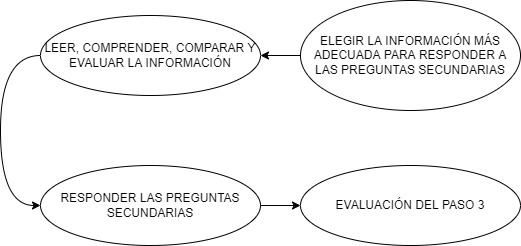
\includegraphics[width=0.70\textwidth]{Cap2/Figuras/Análisis de la información.jpg}
  \caption{Análisis de la información. González (2007)}
  \label{fig:25}
\end{figure}

%------------------------------------------------------------
%	Subpaso 3a: Elegir la información más adecuada para responder las preguntas secundarias
%------------------------------------------------------------

\subsubsection{Subpaso 3a: Elegir la información más adecuada para responder las preguntas secundarias}
\label{secPaso3aCap2}

Como objetivo de este subpaso se tiene el desarrollar la habilidad de selección de información, que responda de mejor manera a las preguntas secundarias. Este subpaso conlleva a prestar especial atención a la información que realmente es útil, lo cual lo vuelve uno de los pasos más complejos del Modelo Gavilán.

Por lo general, cuando se realiza un proceso de copy-paste con una fuente de información, se analiza superficialmente cuál es la información que resuelve de mejor manera el problema de información. En este subpaso, se analiza la selección de párrafos y datos que responden de mejor manera a las preguntas secundarias, con la diferencia de que no se copia y se pega la información, sino que se extrae sólo lo importante y relevante para la investigación.

% REFERENCIA
González (2007), señala que una estrategia para poder seleccionar de manera eficiente la información es considerar los siguientes puntos:

\begin{itemize}
  \item Determinar y preguntarse qué es lo que se requiere saber de la pregunta secundaria en cuestión. Es decir, identificar los fragmentos de información que dan respuesta a las preguntas.
  \item Reflexionar y seleccionar las respuestas que son más aptas para responder la pregunta secundaria y marcar o almacenar el fragmento correspondiente . Es importante que a la par de la selección de información, se incluya la referencia de dónde se obtuvieron dichos datos.
  \item Repetir el proceso con cada una de las preguntas secundarias, usando los fragmentos de información encontrados.
\end{itemize}

Retomando el ejemplo de investigación, se puede ver el ejemplo de la Tabla \ref{tab:t5}

\begin{table}[H]
  \begin{center}
    \begin{tabular}{ | p{2cm} | p{4cm} | p{7cm} | p{3cm} | }
      \hline
      EXTRACTO & PREGUNTA SECUNDARIA & RESPUESTA & REFERENCIA \\ \hline
      1 & ¿Qué es el trauma matemático? & Es la manifestación de miedo o temor por equivocarse, enfocado a contextos relacionados a matemáticas &
      Fuente 1
      \begin{itemize}
        \item Párrafo 5
      \end{itemize}
       \\ \hline

      2 & ¿Quien definió el significado de trauma matemático? & Definido en este artículo por Jennifer Ruef &
      Fuente 1
      \\ \hline
    
      3 & ¿Cuándo se definió el trauma matemático? & La investigación y la definición surgen a partir de la intriga del origen de la dificultad por aprender matemáticas &
      Fuente 1
      \begin{itemize}
        \item Párrafo 2
        \item Párrafo 3
      \end{itemize}
       \\ \hline

      4 & ¿Quienes pueden ser afectados por el trauma matemático? & El problema es que el alumno sigue reprobando matemáticas a pesar de ser una materia básica y sobre todo cotidiana; la razón de lo anterior se debe a que todos los días usamos las matemáticas. &
      Fuente 2
      \begin{itemize}
        \item Página 3
        \item Párrafo 1
      \end{itemize}
       \\ \hline

      5 & ¿Quienes pueden ser afectados por el trauma matemático? & Cuando las personas comparten sus historias conmigo, hay temas comunes. Estos incluyen a alguien diciéndoles que $"$no eran buenos en matemáticas$"$. Uno de los mayores desafíos a los que se enfrentan los educadores de matemáticas de Estados Unidos es ayudar a la gran cantidad de maestros de primaria que se enfrentan a un 'trauma matemático' &      
       Fuente 1
       \begin{itemize}
         \item Párrafo 2
         \item Párrafo 4
       \end{itemize}
        \\ \hline
      
      6 & ¿Cómo puede presentarse el trauma matemático? & pánico por las pruebas de matemáticas programadas, o quedando atrapado en algún tema de la materia y luchando para superarlo &
       Fuente 1
       \begin{itemize}
         \item Párrafo 2
       \end{itemize}
        \\ \hline
      
      7 & ¿Cómo puede presentarse el trauma matemático? & Esto hace que ellos se sientan desmotivados durante su proceso de aprendizaje, por lo que su conducta es de negación hacia las matemáticas al considerar poco probable la adquisición de los conocimientos. El fracaso, es el mayor factor por el cual las personas le tienen miedo a las matemáticas. El fracaso y el miedo dan mucho que decir al momento de pasar al pizarrón o sacar una nota no aprobatoria en el examen. Así mismo el rechazo de la sociedad puede afectar porque si el alumno no saca calificaciones aceptables &
       Fuente 2
       \begin{itemize}
         \item Página 2
         \item Página 5
         \item Página 10
       \end{itemize}
        \\ \hline

    \end{tabular}
  \end{center}
\end{table}

\begin{table}[H]
  \begin{center}
    \begin{tabular}{ | p{2cm} | p{4cm} | p{7cm} | p{3cm} | }
      \hline
      8 & ¿Cómo puede presentarse el trauma matemático? & Una de las razones de esta $"$ansiedad numérica$"$ tiene que ver con la forma en que se enseña la matemática, basada en la memorización y las fórmulas jeroglíficas, los tests matemáticos y la naturaleza blanco/negro de los problemas que solo admiten una respuesta correcta. Sacar malas notas en los exámenes resulta ser una bomba fulminante. &
        Fuente 3
        \begin{itemize}
          \item Párrafo 3
        \end{itemize}
         \\ \hline
      
      9 & ¿Qué tipo de ejercicios se pueden realizar para mejorar en matemáticas? & que hacen que las personas jueguen con números, como Sudoku, KenKen o ciertos juegos de cartas, crean una necesidad intelectual de usar datos matemáticos que ayudan a los niños a desarrollar la fluidez de los datos. Pedirles a los niños que expliquen su pensamiento, usando palabras, imágenes u objetos, valida la importancia de sus ideas. &
         Fuente 1
         \begin{itemize}
           \item Párrafo 12
         \end{itemize}
          \\ \hline

      10 & ¿Qué estrategias se pueden seguir para practicar ejercicios matemáticos? & Replantear los errores como exploraciones. No tener una respuesta correcta no significa que todo pensamiento sea incorrecto. Pedirles a los niños que expliquen su pensamiento también ayuda a comprender lo que saben ahora y lo que podrían aprender a continuación. Segundo, no hagas daño. Es importante que los padres eviten enviarles a los niños mensajes de que no son matemáticos. &
      
          Fuente 1
          \begin{itemize}
            \item Párrafo 13
            \item Párrafo 14
          \end{itemize}
           \\ \hline

    \end{tabular}
    \caption{Ejemplo de estrategias del subpaso 3a del Modelo Gavilán.}
    \label{tab:t5}
  \end{center}
\end{table}

%------------------------------------------------------------
%	Subpaso 3b: Leer, entender, comparar, y evaluar la información seleccionada
%------------------------------------------------------------

\subsubsection{Subpaso 3b: Leer, entender, comparar, y evaluar la información seleccionada}
\label{secPaso3bCap2}

El objetivo de este subpaso es desarrollar las habilidades para encontrar relaciones entre los fragmentos de información seleccionados, de tal forma que se pueda determinar, para cada una de las preguntas secundarias, qué información puede fungir como complemento, comparación, verificación, ejemplo, o dato extra.

Esta es una fase en la que se determinan relaciones entre la información seleccionada de los diferentes recursos para evaluar si es necesario profundizar en dicha fuente o si es necesario considerar otros aspectos del tema. En caso de ser necesario, se consideran otros aspectos o se profundiza en la fuente actual, pero también se puede recurrir a la consulta de más fuentes de información, mismas que se evalúan y seleccionan como en el paso dos del Modelo Gavilán, referente a la búsqueda y evaluación de fuentes.

Cabe resaltar que dados los posibles casos de profundización o ampliación de información, se debe retornar a pasos anteriores y repetir cada una de las fases del paso dos, hasta que se concrete la información suficiente y necesaria para tener como resultado una investigación completa, clara y con información de calidad.

En la Tabla \ref{tab:t6} se muestra un ejemplo de comparación y evaluación de los extractos obtenidos en el subpaso 3a.

\begin{table}[H]
  \begin{center}
    \begin{tabular}{ | p{4cm} | p{5cm} | p{7cm} | }
      \hline
      EXTRACCIONES & COMPARACIÓN & EVALUACIÓN \\ \hline
      1 y 2 & Complemento & Información relevante para la investigación, ya que proporciona una definición del trauma matemático y su autor. \\ \hline
      3 & Complementario a los extractos 1 y 2 & La información de cómo surge el trauma matemático no es relevante para la investigación, por lo que este se puede omitir. \\ \hline
      4 y 5 & Complemento & Información relevante para la investigación, que contiene los efectos del trauma matemático \\ \hline
      7 y 8 & Ejemplo & Información relevante de presentación de trauma matemático, así como ejemplos. \\ \hline
      9 y 10 & Ejemplo & Información relevante de cómo tratar el trauma matemático y ejemplos de ejercicios \\ \hline
    \end{tabular}
    \caption{Ejemplo de estrategias del subpaso 3b del Modelo Gavilán.}
    \label{tab:t6}
  \end{center}
\end{table}

%------------------------------------------------------------
%	Subpaso 3c: Responder las preguntas secundarias
%------------------------------------------------------------

\subsubsection{Subpaso 3c: Responder las preguntas secundarias}
\label{secPaso3cCap2}

El objetivo principal de este subpaso es desarrollar las estrategias para que el estudiante adquiera la habilidad para responder a cada una de las preguntas secundarias con sus propias palabras.

En este punto del Modelo Gavilán, el estudiante ya conoce las respuestas a cada una de las preguntas secundarias, así como posibles complementos, ejemplos e incluso diferentes puntos de vista. Esta información permite tener una idea del tema general, así como aspectos específicos que son relevantes para la investigación. Los fragmentos recabados sobre las respuestas a las preguntas y la información extra, faculta al estudiante para poder responder cada pregunta secundaria con sus propias palabras, así como desarrollar una aproximación a la estructura de la cada una de las respuestas.

Al responder las preguntas secundarias con palabras propias, se demuestra y se refleja un entendimiento del tema, así como un buen proceso de análisis de la información. Además se muestra el razonamiento que se realiza por parte del estudiante para manifestar el conocimiento aprendido durante este paso.

En la Tabla \ref{tab:t7} se muestra un ejemplo de posibles respuestas de estudiantes a cada una de las preguntas secundarias.

\begin{table}[H]
  \begin{center}
    \begin{tabular}{ | p{8cm} | p{8cm} | }
      \hline
      PREGUNTA SECUNDARIA & RESPUESTA CON PALABRAS DEL ESTUDIANTE \\ \hline
      ¿Qué es el trauma matemático? & Es la fobia o temor por equivocarse al resolver ejercicios matemáticos. \\ \hline
      ¿Quién definió el significado de trauma matemático? & La profesora Jennifer Ruef. \\ \hline
      ¿Cuándo se definió el trauma matemático? & Surgió a partir del cuestionamiento de porqué a algunos de los estudiantes se les complican las matemáticas. \\ \hline
      ¿Quiénes pueden ser afectados por el trauma matemático? & Todos en general, especialmente estudiantes y algunos profesores de matemáticas. \\ \hline
      ¿Cómo puede presentarse el trauma matemático? & Puede presentarse como miedo, rechazo por parte de compañeros y familiares. También puede presentarse como inseguridad de la capacidad de poder resolver problemas matemáticos, lo cual causa desmotivación por querer aprender. \\ \hline
      ¿Qué tipo de ejercicios se pueden realizar para mejorar en matemáticas? & Algunos juegos que desarrollen la habilidad matemática, tal como sudokus o cartas. \\ \hline
      ¿Qué estrategias se pueden seguir para practicar ejercicios matemáticos? & Una estrategia es reconocer  que no obtener la respuesta correcta a un problema, no es malo. Por el contrario, está bien equivocarse y aprender de los errores para no cometerlos en los próximos ejercicios. Otra estrategia es evitar decir a los estudiantes que son malos en matemáticas.
       \\ \hline
    \end{tabular}
    \caption{Ejemplo de estrategias del subpaso 3c del Modelo Gavilán.}
    \label{tab:t7}
  \end{center}
\end{table}

%------------------------------------------------------------
%	Subpaso 3d: Evaluación del paso 3
%------------------------------------------------------------

\subsubsection{Subpaso 3d: Evaluación del paso 3}
\label{secPaso3dCap2}

Este paso de evaluación le concierne al tutor a cargo de la valoración de la investigación realizada por el estudiante. En esta evaluación se mide el desarrollo de las habilidades para analizar información a partir de la comprensión, el análisis, la relación y comparación de la información.

Se determina si se cumplieron los objetivos de cada subpaso y se logró el resultado esperado, para dar respuesta correcta y de calidad con palabras propias a las preguntas secundarias, con base en la atención y análisis de las relaciones que existieron entre diferentes fragmentos de información para una sola pregunta.

Los criterios a considerar para la evaluación del análisis de información pueden variar y pueden ser ajustados por el tutor de la investigación. El equipo de EDUTEKA desarrolló una lista de verificación que puede fungir como guía para determinar qué tan bien se lograron los objetivos de los subpasos del tercer paso del Modelo Gavilán, que puede consultarse en EDUTEKA (2007).

%------------------------------------------------------------
%	Síntesis y socialización de la información
%------------------------------------------------------------

\subsection{Síntesis y socialización de la información}
\label{secPaso4Cap2}

El objetivo de este último paso del Modelo Gavilán, es desarrollar las estrategias para que el estudiante pueda adquirir las habilidades necesarias para sintetizar y organizar la información de forma clara y enfocada en el resultado de la investigación.

En esta etapa se busca resolver el problema de investigación a los que se enfrentan los estudiantes al momento de comenzar la búsqueda de información. Para lograr este resultado, se recaba todo el esfuerzo y resultados obtenidos en los pasos anteriores, de tal forma que se pueda estructurar para resolver cada aspecto considerado en las preguntas secundarias y, en conjunto, la pregunta inicial.

Además, se busca que toda la información recopilada, que ya cuenta con cierta estructura, se pueda expresar o representar por el medio de comunicación adecuado, para que la investigación pueda ser entendida por un tercero.

Los subpasos del cuarto y último paso del Modelo Gavilán expresan cada una de las acciones y tareas para desarrollar las habilidades de síntesis y socialización de información. Los pasos del cuarto paso del Modelo Gavilán son los siguientes.

\begin{itemize}
  \item [4a.] Responder la pregunta inicial
  \item [4b.] Elaborar un producto concreto
  \item [4c.] Comunicar los resultados de la investigación
  \item [4d.] Evaluación del paso 4 y el proceso
\end{itemize}

Estos subpasos se siguen como en la Figura \ref{fig:26}.

\begin{figure}[H]
% \begin{figure}
  \centering
  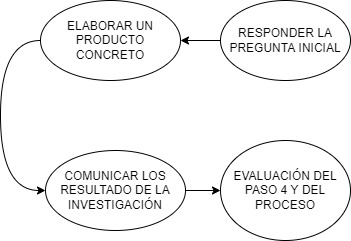
\includegraphics[width=0.60\textwidth]{Cap2/Figuras/Síntesis y socialización de información.jpg}
  \caption{Síntesis y socialización de la información. González (2007)}
  \label{fig:26}
\end{figure}

%------------------------------------------------------------
%	Subpaso 4a: Responder la pregunta inicia
%------------------------------------------------------------

\subsubsection{Subpaso 4a: Responder la pregunta inicia}
\label{secPaso4aCap2}

El objetivo de este subpaso consta de adquirir las habilidades para poder recuperar y relacionar información, para dar respuesta completa a la pregunta inicial del problema de investigación.

Este paso requiere de un análisis profundo para identificar distintos aspectos del problema general y relacionarlos entre sí, para construir una respuesta completa que sea clara, coherente y aporte la información requerida por los criterios de la investigación. Es un proceso de unificación, que surge a partir de las respuestas de las preguntas secundarias para crear un texto que cubra todos los detalles solicitados de un tema, así como aportaciones extras del estudiante.

% REFERENCIA
González (2007), propone una estrategia para organizar la información y conocer los diferentes puntos de un tema. Esta estrategia consiste en elaborar mapas que permitan distribuir y organizar la información en diferentes categorías, tal como un mapa conceptual u otra representación de información. Estas herramientas clarifican la forma en que se distribuye la información y se representa de forma gráfica.

Al construir la representación general con cada fragmento de datos obtenidos en el tercer paso del Modelo Gavilán, se sintetiza la información como una sola para dar una respuesta completa a la pregunta inicial, considerando todos los componentes que apoyan a sostener la investigación obtenida. En consecuencia de la elaboración de esta representación gráfica, se produce un criterio para unificar la información en una sola respuesta completa a la pregunta inicial, así como para encontrar datos faltantes o categorías que podrían complementar la información final.

A continuación se muestra un esquema donde se distribuye la información obtenida en el subpaso 3c del ejemplo  desarrollado en el paso anterior, en la Figura \ref{fig:27}.

\begin{figure}[H]
% \begin{figure}
  \centering
  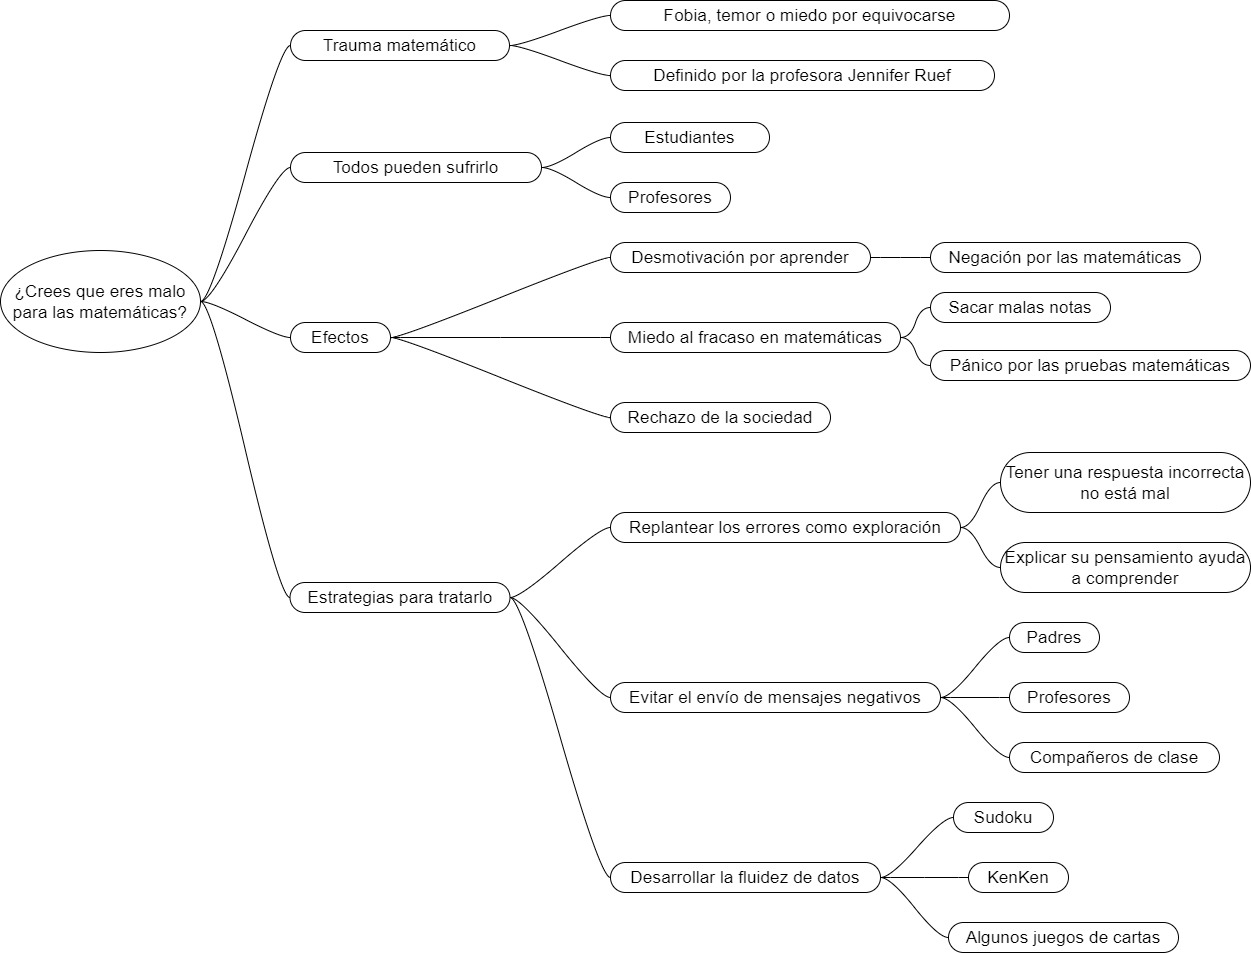
\includegraphics[width=0.70\textwidth]{Cap2/Figuras/Ejemplo de estraregia del subpaso 4a.jpg}
  \caption{Ejemplo de estrategias del subpaso 4a del Modelo Gavilán.}
  \label{fig:27}
\end{figure}

%------------------------------------------------------------
%	Subpaso 4b: Elaborar un producto concreto
%------------------------------------------------------------

\subsubsection{Subpaso 4b: Elaborar un producto concreto}
\label{secPaso4bCap2}

El objetivo de este subpaso es llevar la información recopilada a un producto que cuente con todos los datos necesarios que respondan a la pregunta inicial en forma de ensayo, artículo, mapa conceptual, dibujo, de esquema, video, entre otros.

En esta etapa del cuarto paso, es necesario definir una forma de representar la información, misma que puede estar estipulada por un tutor o en su defecto, ser elegida por el estudiante, considerando la opción más viable para expresar los resultados. Es importante a su vez, asegurar que la información que ya se analizó y organizó, haya sido entendida por el estudiante, con el fin de adquirir los conocimientos esperados en la investigación del tema.

Es valioso mencionar que la información, dependiendo de sus características, se acopla más a un esquema de representación que a otro, por lo que el estudiante puede utilizar diferentes esquemas de representación en el producto final. Es decir, pueden existir combinaciones como mapas en un ensayo, gráficas en un artículo, imágenes en mapas conceptuales, etc.

Por otro lado, dependiendo del tipo de entrega o investigación, esta puede ser construida de forma digital, como una presentación, un video, una imagen, etc., así como de forma física como un dibujo, un ensayo, una tarjeta, etc. Este punto también se encuentra determinado por la elección de un tutor o del estudiante.

Para la elección de estos aspectos, es considerablemente necesario conocer las características con las que cuenta cada esquema de representación de información, para explotar así sus ventajas.

Finalmente, se pone en consideración la forma en que el estudiante adquirió el dominio y comprensión del tema de investigación, ya que no sólo es importante aprender a poner en práctica y adquirir las habilidades del modelo gavilán, sino también aprender contenido útil sobre el tema involucrado en la investigación, de tal forma que se expanda el conocimiento del tema comparado con lo que se conocía antes de la investigación.

Retomando el ejemplo con la información del subpaso anterior, se presenta a continuación un breve reporte en la Tabla \ref{tab:t8}.

\begin{table}[H]
  \begin{center}
    \begin{tabular}{ | p{16cm} | }
      \hline
      RESULTADO FINAL DE LA INVESTIGACIÓN - REPORTE \\ \hline
      ¿Crees que eres malo para las matemáticas? Esto puede ser causa de un trauma matemático. El trauma matemático, definido por la profesora Jennifer Ruef, es el miedo, fobia o temor por equivocarse en ejercicios o la resolución de problemas matemáticos.
      
      El trauma matemático se presenta principalmente en estudiantes y profesores, sin embargo, cualquier persona puede presentar un trauma matemático, provocando desmotivación por el aprendizaje, miedo al fracaso o rechazo por la sociedad. Esto puede causar que el afectado desarrolle una negación por las matemáticas, obtener malas calificaciones o incluso generar pánico en pruebas matemáticas.
      
      Para prevenir y evitar el trauma matemático, se pueden tomar en cuenta los siguientes aspectos:

      \begin{itemize}
        \item Replantear los errores como exploración. Es importante trabajar en la aceptación y la determinación para saber que una respuesta incorrecta en las pruebas de matemáticas no está mal. Por el contrario, se puede explorar y explicar lo que el alumno piensa para comprender mejor los temas, con el fin de aprender de los errores, de tal forma que en una prueba siguiente, ya se tendrá conocimiento para no cometer el mismo error.
        \item Evitar el envío de mensajes negativos. Algunas personas piensan que son malas en matemáticas porque así lo dijo un profesor, algún compañero de clase o incluso los padres. Es importante evitar los comentarios negativos, para no generar angustia y provocar un trauma matemático.
        \item Desarrollar actividades donde se trabaja la fluidez de datos. Para poner en desarrollo y práctica la habilidad matemática, se recomienda realizar actividades donde intervenga el análisis matemático y el proceso de datos, tal como el sudoku, KenKen o algunos juegos de cartas.
      \end{itemize}

      \\ \hline
    \end{tabular}
    \caption{Ejemplo de estrategias del subpaso 4c del Modelo Gavilán.}
    \label{tab:t8}
  \end{center}
\end{table}

%------------------------------------------------------------
%	Subpaso 4c: Comunicar los resultados de la investigación
%------------------------------------------------------------

\subsubsection{Subpaso 4c: Comunicar los resultados de la investigación}
\label{secPaso4cCap2}

En este paso se desarrollan las habilidades para poder expresar la información que se obtuvo en el esquema del subpaso anterior de forma oral, de tal manera que se pueda comunicar como exposición hacia un tutor o un grupo de personas.

Las actividades de este subpaso involucran varios aspectos que pueden manifestar el buen trabajo realizado en los pasos del Modelo Gavilán. Tales como hablar con buen dominio sobre el tema, tener cierta organización en la forma en que se expresan las ideas del tema, conocer datos específicos de un tema general, exponer ejemplos que clarifiquen un tema y finalmente, tener la habilidad de responder todas las dudas o cuestiones que surjan al final de una exposición.

A pesar de tener un documento con toda la información necesaria para responder la pregunta inicial vinculada a un tema, es importante mencionar que en una exposición no todos los datos son relevantes o no es necesario profundizar tanto en ellos, ya que la investigación del esquema del subpaso anterior puede ser muy amplio.

Es primordial recalcar que en una exposición, se tiene por objetivo la comunicación del tema y el tipo de audiencia al que se dirige el conocimiento. González (2007) señala que algunos puntos importantes a considerar en este subpaso son los siguientes.

\begin{itemize}
  \item Comunicar las ideas más generales de forma clara y comprensible para la audiencia.
  \item Generar recursos gráficos que sirvan de apoyo visual para dar un mejor resultado al entendimiento de información.
  \item El uso correcto y claro de ejemplos y analogías con los que la audiencia pueda sentirse identificada para entender el tema.
  \item Considerar, sin excepción, el respeto a los derechos de autor de los recursos de donde se extrae la información.
\end{itemize}

%------------------------------------------------------------
%	Subpaso 4d: Evaluación del paso 4 y el proceso
%------------------------------------------------------------

\subsubsection{Subpaso 4d: Evaluación del paso 4 y el proceso}
\label{secPaso4dCap2}

El objetivo de este último subpaso consiste en evaluar las habilidades obtenidas para poder sintetizar y organizar la información. Además, al ser el último paso del Modelo Gavilán, también se incluye la evaluación del resultado logrado a partir de todo el proceso desde el primer paso hasta este punto.

Tal como en la evaluación de los pasos anteriores, el tutor del estudiante es el encargado de determinar y medir si los objetivos esperados de cada subpaso se concluyeron de forma satisfactoria. Así mismo, el tutor tiene el cargo de evaluar los resultados finales de todo el proceso hecho, siguiendo los pasos del Modelo Gavilán.

Para determinar si los objetivos se cumplieron, se establecen criterios de evaluación establecidos por el mismo tutor, donde se destacan aspectos importantes como un correcto análisis para la síntesis, una buena organización, buen dominio del tema para exposición, la capacidad de comunicar ideas críticas de un tema, entre otros. Algunos aspectos propuestos por el equipo de EDUTEKA, llamado LISTA DE VERIFICACIÓN - EVALUACIÓN PASO 4 (MODELO GAVILÁN), que pueden ser considerados para la evaluación, pueden encontrarse en EDUTEKA (2007). 

Cabe mencionar que los criterios de evaluación establecidos en la lista son un apoyo para la evaluación. El tutor de la investigación puede agregar u omitir criterios a evaluar.

%------------------------------------------------------------
%	Resumen
%------------------------------------------------------------

\section{Resumen}
\label{secResumenCap2}

En este capítulo se define la competencia de manejo de información, como un conjunto de habilidades, conocimientos y actitudes que un estudiante requiere para contextualizar y saber de manera precisa los detalles que se requieren extraer para un tema, así como desarrollar estrategias de búsqueda de la información más apta para utilizar como resultado de una investigación final. Por otra parte, la CMI también tiene el objetivo de desarrollar habilidades para obtener la capacidad de crear preguntas específicas y aplicarlas para concretar o detallar la información filtrada de las mejores fuentes de información.

A su vez, se menciona que una competencia se compone de dos factores: capacidades y actitudes. Por un lado, las capacidades se dividen en otras dos partes: conocimientos, que es todo aquello que se sabe sobre un tema; y las habilidades, que corresponde a la capacidad de usar la información que se sabe para resolver algún problema. Por otra parte, las actitudes se refieren a la buena disposición de lograr un objetivo.

Entre las metodologías para el desarrollo de la CMI, se encuentra la metodología conocida como El Modelo Gavilán, la cual es una metodología que se basa en cuatro pasos principales.

\begin{enumerate}
  \item Definición del problema de investigación.
  \item Búsqueda y evaluación de la información.
  \item Análisis de la información.
  \item Síntesis de la información.
\end{enumerate}

A su vez, cada uno de los pasos mencionados anteriormente, se dividen en subpasos, que proponen el desarrollo de habilidades específicas para poner cumplir los objetivos planteados en la CMI.

Para el desarrollo del proyecto, se toma como referencia el Modelo Gavilán para la construcción de la skill. Los autores del Modelo Gavilán mencionan que las habilidades desarrolladas en cada subpaso fungen como una propuesta para su aplicación, sin embargo, estas pueden ser adaptadas para el funcionamiento más adecuado de la metodología. Es importante mencionar que se considera una adaptación de algunos subpasos del Modelo Gavilán. La adaptación del Modelo Gavilán a la skill será descrita en el capítulo 4.



%------------------------------------------------------------
%	CAPÍTULO III
%------------------------------------------------------------

%------------------------------------------------------------
%	CAPITULO I
%------------------------------------------------------------

\chapter{Diseño de interfaces de usuario basadas en voz}
\label{capIII}

% REFERENCIA
Dix, Finlay, Abowd y Beale (2004), señalan que la interacción entre humano y computadora, es la forma en que un usuario se comunica y se relaciona con un sistema computacional, así como la forma en que un usuario utiliza una computadora como herramienta para resolver o facilitar distintas tareas.

La comunicación entre un usuario y un sistema se logra gracias a un intermediario llamado interfaz. Esta se encarga de realizar las traducciones necesarias para hacer posible la comunicación de una manera más clara e idealmente efectiva, fácil, eficiente y agradable, con el fin de realizar el mejor proceso de comunicación posible. Sin embargo, la interfaz puede fallar al comunicar cierta información, por lo que la comunicación podría ser errónea, confusa y difícil. Es por ello que surgen distintos modelos de interacción, que permiten entender lo que sucede durante la interacción con un sistema y la identificación del posible origen de las dificultades.

Uno de los modelos de interacción más sobresalientes mencionado por Dix, Finlay, Abowd y Beale (2004), se conoce como el Modelo de Norman, basado en el ciclo de ejecución-evaluación de Norman. Este modelo se forma de dos componentes: la ejecución de tareas por parte de la computadora; y la evaluación por parte de los usuarios. Cuando un usuario manifiesta un plan y lo comunica por medio de una interfaz a la computadora, esta se encarga de ejecutar las acciones necesarias para dar una respuesta, misma que se transmite por la interfaz, para finalmente ser evaluada por el usuario. La ejecución  y evaluación involucradas en el proceso de comunicación del Modelo de Norman, se divide en siete fases que se presentan a continuación.

\begin{enumerate}
  \item Establecer el objetivo
  \item Crear la intención
  \item Especificar la secuencia de la acción
  \item Ejecutar la acción
  \item Percibir el estado del sistema
  \item Interpretar el estado del sistema
  \item Evaluar el estado del sistema, dependiendo de los objetivos y las acciones
\end{enumerate}

En las primeras fases, el usuario debe establecer un objetivo sobre aquellas tareas que requiere lograr o satisfacer, mismas que después debe traducir y adaptar para comunicar al sistema. Esta traducción se convierte en una secuencia de acciones que posteriormente se ejecutan en el sistema, lo cual provoca un cambio en el estado del sistema con la respuesta de la solicitud realizada. Estos resultados son interpretados y evaluados por el usuario, tomando en cuenta los objetivos y acciones definidas. Si la evaluación arroja resultados favorables y refleja los objetivos, entonces la interacción entre el usuario y el sistema se considera como exitosa. De lo contrario, el usuario genera un nuevo objetivo y repite todos los pasos, es por ello que el modelo se considera como un ciclo de ejecución y evaluación.

Para ilustrar el proceso descrito anteriormente, supongamos que una persona se encuentra viendo una película y decide comer palomitas de maíz, convirtiendo esto en un objetivo. La intención se crea en forma de poner palomitas de maíz en el microondas. La secuencia de la acción puede ser el hecho de levantarse, colocar las palomitas en el microondas y establecer un tiempo adecuado para la preparación. En caso de que haya alguien cerca del microondas la intención y la secuencia de acción puede modificarse, si la intención se convierte en pedir a alguien que prepare las palomitas. En este ejemplo, el objetivo es el mismo, pero la intención y las acciones pueden variar. Cuando se ejecuta la acción y las palomitas están preparadas, se percibe el cambio de estado con el resultado. A este resultado se le interpreta y evalúa dependiendo de la percepción, es decir, si las palomitas están bien preparadas, entonces el ciclo se ha completado, de lo contrario, se genera un nuevo objetivo dependiendo del resultado, por ejemplo, si las palomitas se quemaron el nuevo objetivo es preparar unas palomitas nuevas, pero si a las palomitas les faltó más tiempo en el microondas, el nuevo objetivo es llevarlas nuevamente al microondas.

Es importante mencionar que durante el proceso pueden surgir eventos inesperados o excepcionales que se dividen en dos categorías: resbalones (slips) y equivocaciones (mistakes). Si el usuario conoce el comportamiento del sistema, así como las respuestas esperadas a las solicitudes y accidentalmente presiona algún botón o ejecuta alguna acción no planeada, entonces se considera como un resbalón. Por otro lado, si el usuario no conoce el sistema por completo y ejecuta alguna acción, recibiendo una respuesta que no esperaba, entonces se considera una equivocación.

Este modelo permite entender de forma más clara e intuitiva la interacción del usuario con el sistema, sin embargo, no detalla la interacción del sistema con el usuario por medio de la interfaz. Existe una extensión del Modelo de Norman, propuesto por Dix, Finlay, Abowd y Beale (2004), que se enfoca en la interacción del sistema por medio de la interfaz. 

La extensión del modelo de Norman para la interacción del sistema con el usuario se divide en cuatro componentes: el sistema, el usuario, las entradas y las salidas. El ciclo asociado a este modelo se compone de cuatro pasos que se muestran a continuación.

\begin{itemize}
  \item Articulación
  \item Rendimiento
  \item Presentación
  \item Observación
\end{itemize}

Los componentes, así como los pasos de transición entre componentes se muestra en la Figura \ref{fig:31}.

\begin{figure}[H]
% \begin{figure}
  \centering
  \includegraphics[width=0.70\textwidth]{Cap3/Figuras/Transacción entre componentes.jpg}
  \caption{Transición entre componentes del Modelo de Norman para sistemas (2004).}
  \label{fig:31}
\end{figure}

El ciclo comienza con el usuario, quien es el encargado de crear un objetivo y una tarea o secuencia de acciones para realizar alguna tarea con ayuda del sistema. La forma en que el usuario comunica al sistema la información necesaria para realizar la tarea se transmite a partir de la articulación. En este paso, el usuario comunica las entradas al sistema por medio de la articulación, pasando al componente de entradas. Estas entradas son llevadas al sistema por medio del rendimiento, el cual es un proceso que se encarga de traducir las entradas en operaciones. El sistema se encarga de transmitir las operaciones y todos los datos abstractos en una forma que pueda ser entendida por el usuario por medio de la presentación. Finalmente, estas salidas son mostradas o dadas a conocer al usuario por medio de una interfaz, en donde el usuario puede consultar los resultados de la tarea por medio de la observación.

Tal como se mencionó anteriormente, esta extensión del Modelo de Norman está enfocado en la interacción del sistema con el usuario, es decir, analizar los posibles puntos de dificultad del sistema para el usuario. En el primer paso de este modelo, es importante que el usuario pueda comunicar sus objetivos al sistema por medio de una articulación que pueda entender el sistema. Supóngase que el objetivo de un usuario es seleccionar un estado de la república mexicana. Dependiendo del sistema, el usuario podría articular esta información por medio de la escritura del estado, sin embargo, esto está vulnerable a muchas dificultades, ya que un estado se podría escribir en mayúsculas, minúsculas, una combinación de ambas, por sus siglas o incluso escribir un texto que no es un estado. Otra forma de articular el mismo objetivo del usuario sería con una lista que contiene todos los estados válidos. En este caso, el usuario puede seleccionar un estado en un lenguaje que puede ser entendido y controlado por el sistema, ya que está limitado por sí mismo. En este paso se puede determinar qué tan buena es la facilidad de articulación que brinda el sistema para poder comunicar las entradas para realizar diferentes tareas.

En el siguiente paso las entradas pasan al sistema por medio del rendimiento. Este paso se enfoca principalmente en el manejo de los estímulos del sistema como respuesta a una solicitud con entradas específicas. Es decir, se determina el alcance de respuesta del sistema con entradas determinadas por el usuario. Por ejemplo, cuando se requiere ingresar información importante en un asistente basado en voz, tal como números de cuenta, el alcance para el estado de ingreso de información por medio de voz no está disponible por cuestiones de seguridad. Por otro lado, el alcance de ingreso de información importante sí es alcanzado por medio de la aplicación asociada al asistente. En el paso de rendimiento se puede determinar cuáles son las acciones que pueden o no ser alcanzadas en distintas circunstancias, lo cual, está directamente ligado a la implementación del sistema. Para el ejemplo anterior, el esfuerzo extra para el usuario es un control de seguridad que provee el sistema y que puede verse afectado en costo de implementación.

El paso de presentación consiste en traducir y mostrar los resultados de la consulta y la interacción anterior con el sistema. La traducción mostrada debe ser traducida de tal forma que se pueda transmitir de forma clara y 	fácil al usuario a partir de las herramientas con las que cuenta la interfaz. Es un proceso en el que se acopla la traducción del sistema hacia el usuario a través de la interfaz. Si la interfaz cuenta con pantalla, la información se puede transmitir visualmente, de lo contrario, se tendría que transmitir de otra manera, tal como información táctil o auditiva. Por otra parte, en este paso también se evalúa si la cantidad de información, así como la forma en que se presenta, es la más adecuada para facilitar la comunicación con el usuario. Finalmente, el usuario interpreta y evalúa la respuesta del sistema, donde se pueden tomar en cuenta puntos importantes de la interacción con el sistema como la facilidad de comunicación y el entendimiento de la respuesta por parte del sistema.

%------------------------------------------------------------
%	Interfaces de usuario
%------------------------------------------------------------

\section{Interfaces de usuario}
\label{InterfacesUsuarioCap3}

En términos tecnológicos, una interfaz de usuario es un medio que permite la interacción de un sistema interactivo entre una computadora y un usuario. Una interfaz de usuario se vuelve entonces, un intermediario entre la comunicación de mensajes de un sistema y una persona.

Una interfaz de usuario tiene como objetivo facilitar las necesidades o la realización de alguna tarea o acción específica, por lo que la comunicación entre el sistema y el usuario tiene que ser clara y fácil de entender. Esto se logra a partir de una interfaz usable, universal, sencilla de entender y que pueda generar resultados útiles.

% REFERENCIA
Shneiderman (2016) señala que los diseñadores de interfaces de usuario han desarrollado normas, a partir de la experiencia y práctica, para mejorar y lograr el diseño más adecuado de una buena interfaz de usuario. Estas normas se dividen en tres categorías, dependiendo de su nivel de importancia: guías, principios y teorías.

\begin{itemize}
  \item \textbf{Guías}: son consejos de bajo nivel sobre las buenas prácticas y precaución de peligros al momento de diseñar una interfaz de usuario.
  \item \textbf{Principios}: son estrategias o reglas de medio nivel, que permiten analizar y comparar las alternativas de diseño de la interfaz de usuario.
  \item \textbf{Teorías}: son marcos de alto nivel, que son fuertemente aplicables durante la etapa de diseño y evaluación de la interfaz de usuario. Por otra parte, estos marcos también apoyan el diseño de la comunicación y enseñanza del sistema para su mejor manejo.
\end{itemize}

% REFERENCIA
Un documento de guía, el cual proporciona consejos sobre las buenas prácticas, ayuda durante el proceso de desarrollo, proporcionando un mecanismo en el que se define el lenguaje y la terminología usada en un sistema. Shneiderman (2016) señala que los documentos de guía, promueven la consistencia en el diseño, apariencia y la secuencia de acciones. Así mismo, estos documentos almacenan las mejores prácticas de diseño derivadas de la experiencia y estudios empíricos, en los que se pueden incluir ejemplos y contraejemplos.

A continuación, se presentan algunos documentos de guía para diferentes aspectos de las interfaces de usuario.

\begin{itemize}
  \item \textbf{Navegación en la interfaz.} En ocasiones, la navegación en una interfaz de usuario puede ser complicada y confusa para algunos usuarios. El documento de guía presentado por el gobierno de Estados Unidos para el diseño de navegación en interfaces propone algunas recomendaciones como las siguientes:
  \begin{itemize}
    \item Estandarizar las secuencias para realizar tareas en un sistema.
    \item Asegurar que los mensajes mostrados sean descriptivos. 
    \item Utilizar encabezados descriptivos y únicos.
    \item Utilizar radio buttons (botones de radio) para elecciones exclusivas.
  \end{itemize} 
  \item \textbf{Organización de elementos desplegados.} Un documento de guía enfocado a la organización de elementos de la interfaz, desarrollado por Smith y Moiser en 1986, ofrece cinco objetivos principales para presentar los datos o información en una interfaz, de tal forma que la organización sea la más adecuada y factible para el mejor control del sistema. Estos cinco objetivos se muestran a continuación:
  \begin{itemize}
    \item Consistencia de información presentada.
    \item Mostrar la información más adecuada y eficiente para el usuario.
    \item Presentar la cantidad mínima de datos.
    \item Compatibilidad entre la información mostrada con la información de entrada.
    \item Flexibilidad de recuperación de datos para el usuario.
  \end{itemize}
  \item \textbf{Obtención de atención del usuario.} El documento de guía llamado Wickens et al., creado en el año 2012, se enfoca en definir algunas guías para lograr obtener la atención del usuario. Algunos de estos consejos se muestran a continuación.
  \begin{itemize}
    \item Subrayar, encerrar, señalar con una flecha o utilizar cualquier forma de marcado para resaltar información relevante durante el proceso.
    \item Utilizar hasta cuatro diferentes tamaños para los elementos y usar el más grande para atrapar la atención del usuario.
    \item Elección de fuentes. Utilizar hasta tres diferentes tipos de fuentes.
    \item Utilizar tonos suaves para retroalimentación positiva y tonos más fuertes para condiciones de emergencia o error.
  \end{itemize}
  \item \textbf{Facilitar la entrada de datos o información de los usuarios.} Un ejemplo de documento de guía enfocado a la entrada de datos es el documento creado por Courtesy of MITRE Corporate Archives, en 1986. El cual propone algunos consejos como los que siguen:
  \begin{itemize}
    \item Consistencia en las transacciones de los datos de entrada.
    \item Mínima cantidad de acciones para la entrada de datos del usuario.
    \item Mínima cantidad de memoria cargada en el usuario.
    \item Compatibilidad de los datos de entrada con la información desplegada en la interfaz.
    \item Flexibilidad en el control de los datos de entrada.
  \end{itemize}
\end{itemize}

Como se muestra anteriormente, las guías se enfocan a cierto rubro de la interfaz y fungen como consejos para ser aplicados de forma limitada. Por otra parte, los principios tienen un enfoque más aplicable y duradero para el diseño de interfaces. Algunos principios están relacionados en los cinco estilos primarios de interacción, presentados a continuación.

\begin{itemize}
  \item \textbf{Manipulación directa.} Es la representación visual del mundo al momento de realizar una acción. Se busca simplificar las tareas con la representación de objetos familiares para el usuario.
  \item \textbf{Navegación y selección de menú.} Se determina una estructura clara para tomar decisiones para realizar las tareas definidas en el sistema. Asimismo, brindan una estrategia para garantizar un diseño consistente.
  \item \textbf{Llenado de formularios.} Este tipo de interacción está más enfocado a usuarios con más experiencia y conocimiento de los sistemas, ya que se debe tener conocimiento de los valores permitidos de entrada.
  \item \textbf{Lenguaje de comandos.} Brinda a los usuarios una sensación de control sobre el sistema, en la cual se aprende la sintaxis y se expresan posibilidades complejas sin la necesidad de instrucciones de uso.
  \item \textbf{Lenguaje natural.} Se implementan, por lo general, cuando las tareas requeridas por un usuario son diversas, tal como uso de contexto, sensores, gestos, comandos hablados, sonido, etc.
\end{itemize}

Los cinco estilos primarios de interacción tienen ventajas y desventajas, dependiendo del tipo de interfaz que se requiera diseñar. En particular, la ventaja que menciona Shneiderman sobre el estilo primario de interacción de lenguaje natural es que alivia la carga de aprendizaje de sintaxis del sistema. Por otro lado, una desventaja que menciona, es que requiere diálogos de aclaración detallados.

Además, existen unas reglas fundamentales que forman parte de los principios del diseño de interfaces de usuario, conocidas como \textit{Las ocho reglas de oro del diseño de interfaces}. Estas ocho reglas se presentan a continuación.

\begin{enumerate}
  \item \textbf{Esforzarse por la consistencia.} Deben definirse secuencias consistentes de acciones para situaciones similares.
  \item \textbf{Usabilidad universal.} Reconocer las necesidades de diversos usuarios, facilitando la transformación de contenido. Es decir, considerar la inclusión de funcionalidades para usuarios principiantes y expertos en el uso del sistema.
  \item \textbf{Mostrar comentarios informativos.} Dar retroalimentación para cada acción del usuario, en donde la respuesta sea modesta para acciones menores, mientras que para las acciones importantes, la respuesta debe ser sustancial y suficientemente detallada.
  \item \textbf{Diseñar diálogos para el cierre de acciones.} La secuencia de cualquier acción del sistema debe presentar un inicio, un punto medio y un final. Esto brinda una sensación de alivio, y satisfacción de logro para realizar las siguientes acciones.
  \item \textbf{Prevención de errores.} Implementar un sistema preventivo de errores para que el usuario no pueda cometer errores graves, y en caso de ocurrir, proveer instrucciones simples, constructivas y específicas para su recuperación.
  \item \textbf{Permitir un fácil retroceso de acciones.} Las acciones deben ser reversibles en lo posible, con el fin de aliviar la ansiedad de los errores que pudieran ocurrir. Esto brinda la posibilidad de deshacer acciones no esperadas por el usuario.
  \item \textbf{Mantener el control en los usuarios.} Cuando los usuarios ya conocen el manejo de una interfaz, no quieren cambios en el comportamiento que ya es familiar, por lo que se determina la familiaridad de las acciones de la interfaz si hay cambios en el diseño.
  \item \textbf{Reducir la carga de memoria a corto plazo.} El procesamiento de información en memoria a corto plazo de los seres humanos es limitado, por lo que es requerido que los usuarios eviten recordar información del sistema que usarán próximamente en otra parte del flujo del sistema.
\end{enumerate}

Finalmente, las teorías representan un marco con fundamentos fuertemente aplicables a las interfaces de usuario. Existen diferentes tipos de teorías que se presentan a continuación:

\begin{itemize}
  \item \textbf{Descriptivas.} Son útiles para desarrollar terminología consistente para un sistema.
  \item \textbf{Explicativas.} Describen la secuencia de eventos de un sistema, en el que se procura desarrollar la causa y efecto de las acciones.
  \item \textbf{Descriptivas.} Brindan una guía para tomar decisiones del diseño de forma más clara.
  \item \textbf{Predictivas.} Permite comparar los diseños propuestos, considerando el tiempo de ejecución, las tasas de error, o niveles de confianza.
\end{itemize}

Asimismo, algunas teorías también se enfocan en determinar una guía para la evaluación y el diseño de las interfaces de usuario. Estos se dividen en teorías micro-HCI y macro-HCI.

Las teorías micro-HCI se concentran en el rendimiento que puede ser medido en la interfaz, tal como la velocidad y los errores que pueden ocurrir en múltiples tareas. Entre estas teorías se encuentran las siguientes:

\begin{itemize}
  \item \textbf{Diseño por niveles.} Comienza con un diseño de alto nivel, que posteriormente se adapta a acciones más pequeñas.
  \item \textbf{Etapas de acción.} Considera el comportamiento del usuario a medida que manejan el sistema para lograr sus objetivos.
  \item \textbf{Consistencia.} Se considera la consistencia presentada en íconos, colores, formas, respuestas u opciones del sistema.
\end{itemize}

Por otro lado, las teorías macro-HCI se enfocan a casos resultantes de la experiencia del usuario durante semanas usando una interfaz de usuario, en las que se evalúan contextos reales. Estas teorías consideran los siguientes aspectos:

\begin{itemize}
  \item \textbf{Contextualizar.} Apoyar a los usuarios que se encuentran envueltos en un ambiente emocional, físico y social.
  \item \textbf{Dinámico.} Se enfoca al diseño para la evolución del comportamiento conforme el usuario avanza en los niveles del sistema.
\end{itemize}

%------------------------------------------------------------
%	Interfaces de usuario basadas en voz
%------------------------------------------------------------

\section{Interfaces de usuario basadas en voz}
\label{InterfacesUsuarioBasadasVozCap3}

%------------------------------------------------------------
%	Interacción basada en voz
%------------------------------------------------------------

\subsection{Interacción basada en voz}
\label{InteraccionBasadaVozCap3}

Existen cinco sentidos que puede percibir el ser humano: vista, oído, tacto, gusto y olfato, donde predomina el sentido de la vista al diseñar una interfaz de usuario, por lo que los sistemas utilizan elementos visuales como principal medio de presentación.

% REFERENCIA
Dix, Finlay, Abowd y Beale (2004), señalan que las interfaces de usuario basadas en voz son un tipo de interfaces inteligentes, también conocidas como interfaces multimodales, las cuales reciben este nombre por la combinación de diferentes canales de presentación basados en los cinco sentidos del ser humano. Es decir, las interfaces inteligentes o multimodales son un tipo de interfaces que permiten percibir y presentar información mediante estímulos visuales, auditivos, táctiles, gestuales, entre otros. Este tipo de interfaces tiene el objetivo de mejorar la interacción entre el sistema y el usuario, con el fin de facilitar la solución a un problema o una tarea.

Cada uno de los canales que pueden ser aplicados a una interfaz inteligente tienen la capacidad de transmitir diferentes percepciones al usuario. El canal auditivo, que se basa en el sonido, permite monitorear los eventos que rodean a un usuario, reaccionando a los ruidos o reproduciendo señales que cambien la atención del usuario. Este canal también permite tener un efecto emocional o más directo por medio de conversaciones auditivas o música, por lo que es capaz de alterar estados de ánimo, crear imágenes visuales y evocar escenas o atmósferas en la mente del usuario.

Por otro lado, el tacto permite representar la retroalimentación táctil que actualmente se aplica en algunas herramientas comunes que se pueden encontrar en automóviles, instrumentos musicales o cualquier herramienta que requiere una interacción con el tacto. Este sentido puede crear un vínculo estrecho entre los individuos con la gran información no verbal que recibe. Este sentido puede ser aprovechado en las interfaces de usuario que están relacionados a las simulaciones, tal como simular el manejo de un avión, simular tocar un instrumento, entre otros.

Los sentidos del gusto y el olfato permiten a un usuario apreciar información útil de la vida cotidiana, tal como verificar si los alimentos están en buen estado, detectar los primeros signos de peligro, entre muchos otros. Estos sentidos permiten al usuario obtener información de su entorno que pueden causar placer o desagrado.

El ambiente con el que interactúa un usuario es multisensorial, en donde cada sentido proporciona diferentes tipos de información del mundo. La interacción entre un usuario con el mundo que nos rodea mejora con diferentes percepciones multisensoriales, por lo que los sistemas interactivos que manejan más de un canal de percepción tienen la capacidad de brindar una interacción más nutrida, que permite ajustar un sistema de interacción más apropiado a las capacidades de los usuarios.

Las interfaces inteligentes, además de asemejar una interacción humano-computadora más natural, también generan sistemas redundantes, en donde se brinda la misma información por diferentes canales de percepción. La redundancia tiene como objetivo proporcionar una experiencia equivalente a todos los usuarios, sin importar su canal principal de interacción.

% REFERENCIA
En particular, una interfaz basada en voz, es un tipo de interfaz inteligente que apoya su interacción principalmente en el canal auditivo, tanto desde el usuario como de la interfaz. Dix, Finlay, Abowd y Beale (2004), señalan que las interfaces basadas en voz permiten el acceso a usuarios con discapacidades visuales, acceder a información en ambientes poco iluminados, así como hacer útil el funcionamiento de diferentes tipos de aplicaciones que no ocupan espacio en una pantalla para mostrar información.

%------------------------------------------------------------
%	Procesamiento de la voz
%------------------------------------------------------------

\subsection{Procesamiento de la voz}
\label{ProcesamientoVozCap3}

Dix, Finlay, Abowd y Beale (2004), señalan que el sonido es una herramienta fundamental para mejorar los criterios de usabilidad. Señalan que existe evidencia experimental que muestran que la confirmación al presionar teclas o generar un click por medio de audio, reduce los errores en un sistema. Otra ventaja en la usabilidad está enfocada en la rama de videojuegos, ya que las pruebas experimentales muestran que los jugadores obtienen un menor puntaje cuando el sonido no está, a comparación de cuando el audio se encuentra presente. 

El sonido en una interfaz puede ser producido por ruido, audio, música, discursos, entre otros. Existen dos tipos de sonidos en los que se dividen todas las categorías anteriores: sonidos de voz y \textit{no voz}. El sonido de voz es aquel que es producido por la voz de un individuo y transmite información o mensajes por medio del sentido de habla, mientras que los sonidos de \textit{no voz} son aquellos que son producidos por ruido, melodías o todo aquello que no sea producido por el sentido del habla. Cabe mencionar que puede haber una combinación de los dos tipos de sonido mencionados, como podcast, canciones, discursos con música de fondo, etcétera.

El habla es uno de los sentidos fundamentales para comunicar información, que se desarrolla desde temprana edad al imitar el habla de todas las personas que nos rodean. El proceso de aprender a hablar es complejo y estructurado, por lo que generar la síntesis del habla por medio de una computadora se vuelve un desarrollo complicado. Por ejemplo, cuando se comienza a aprender un nuevo idioma, es fundamental conocer las reglas gramaticales, que proveen principalmente la estructura de cómo se componen las frases, con el fin de comunicarse con alguien que también conozca la estructura del habla. El diseño de comunicación por voz entre un usuario y un sistema es similar, en donde se debe $"$enseñar$"$ a la computadora a manejar las estructuras del lenguaje para poder comunicarse de la forma más natural posible.

Es primordial conocer la estructura del idioma en el que estará basada la interfaz, ya que con este conocimiento, se trata de lograr la mejor comunicación e interacción posible entre el usuario y el sistema de forma natural. Un posible conjunto de puntos importantes que son necesarios saber sobre el idioma, son los fonemas con los que se compone \footnote{Un fonema es la unidad mínima de sonido de un lenguaje hablado. Cada fonema representa un sonido distinto.}, el énfasis, el acento, las pautas, e incluso el tono en el que se transmite un mensaje para no modificar el significado de un enunciado. Al conocer la estructura del idioma (sintaxis) y la forma en que los puntos anteriores alteran su significado (semántica), es posible lograr la mejor forma de comunicación, donde se reconoce de mejor forma la recepción de mensajes del usuario y se comunica de forma correcta un mensaje de la interfaz al usuario.

Por otro lado, la percepción del sonido, que está relacionado al reconocimiento de voz por computadora, se vuelve complicada con problemas como la detección del ruido de fondo, ya que puede interferir al introducir sonidos que distorsionan el mensaje original. Otro problema es la introducción de pausas o muletillas como $"$ummm$"$, $"$este...$"$, $"$emmm$"$, etc, ya que el reconocimiento de voz podría detectar estos fragmentos de entrada como información útil para el sistema. Finalmente, otro problema que puede distorsionar la entrada, son los acentos tradicionales de cada región, ya que la variación del acento transforma las entradas del sistema de reconocimiento, ya que cada variación puede ser diferente con la forma en que se transmiten ciertos mensajes, así como el cambio de vocabulario.

Otro aspecto importante a considerar con el sonido producido por el habla, es la síntesis de la voz. Este aspecto se refiere al principio de poder tener una conversación natural con una computadora, en el que se refleje la interacción diaria entre dos personas. Uno de los retos más importantes para el reconocimiento de voz, es la sensibilidad a las variaciones y entonación del habla, por lo que la forma de transmitir información por medio de la interfaz debe ser clara y objetiva. Asimismo, la transmisión de voz de forma natural, desde la interfaz basada en voz, resulta difícil de adaptar con tonos monótonos y robotizados, en los que es muy probable notar la ausencia de sentimientos o entonación durante la emisión de mensajes. Para lograr una conversación natural entre una computadora y un usuario, es primordial conocer la forma de interacción del usuario, tomando en cuenta los puntos anteriores, así como el lenguaje, el vocabulario, modismos, frases e incluso la entonación o forma en que se transmiten los mensajes en una conversación cotidiana, con el fin de que el usuario pueda realizar sus tareas con el sistema, en un ambiente en el que se sienta identificado, satisfecho y cómodo.

Otro punto a considerar durante el diseño de las interfaces de usuario basadas en voz, está relacionado a la consulta y exploración del sistema. Al ser una interfaz cuyo canal principal es la voz, se vuelve complicado consultar información o acceder a la exploración general del sistema. En una interfaz visual, el usuario puede tener un panorama general de las tareas que puede realizar utilizando la interfaz, sin embargo, con la ausencia del sentido visual, las funcionalidades de la interfaz deben ser explicadas de forma sencilla y objetiva al usuario. Durante la realización de una actividad con un sistema basado en voz, es valioso tener un sistema de asistencia en el que se lleve paso a paso al usuario para lograr satisfactoriamente la finalización de la tarea. Para ello, durante el diseño de una interfaz basada en voz se debe considerar la división y las pautas que tomará cada actividad para no saturar de información al usuario y no olvide fácilmente el proceso tomado para realizar una tarea.

% REFERENCIA
Dix, Finlay, Abowd y Beale (2004), consideran otro tipo de voz hablada en una interfaz de usuario que no requiere el reconocimiento de voz para hacer funcionar la interacción de la interfaz, este tipo de voz hablada la denominan voz no interpretada. La cual consiste en mensajes pregrabados que son reproducidos en cada uno de los procesos con los que cuenta el sistema, con el fin de complementar o reemplazar información visual. Este tipo de voz hablada es generalmente usada en museos, con el propósito de que los espectadores comprendan de forma sencilla e interactiva el contenido de una sala. Este mecanismo es usado en interfaces que cuentan con un canal visual con el que puede interactuar el usuario para conocer información, y que al recibir retroalimentación de las funcionalidades, se retorna una salida visual y auditiva con la información pregrabada por voz. Al ser grabaciones hechas por una persona, por lo general tienen una entonación y pronunciación humana natural. Este sistema de grabaciones, puede resultar muy útil para interfaces especializadas para aplicaciones colaborativas o para anotaciones de audio que fungen como recordatorios, así como para sentir mayor empatía con la retroalimentación de un sistema al contar con una conversación más natural. Una de las aplicaciones más cotidianas se puede encontrar en las mesas de ayuda telefónica en compañías telefónicas, bancos o asistentes en tiendas virtuales dedicadas a la atención de clientes.

Los sonidos de voz dependen del idioma en que se requiera transmitir la información, por lo que se vuelve una labor complicada la extensión del funcionamiento de un sistema en diferentes idiomas. Los sonidos considerados como \textit{no voz}, tienen ciertas ventajas que pueden enriquecer la forma de interacción entre los usuarios y una interfaz. Como estos sonidos no dependen de la voz, se puede aprovechar como respuesta en el uso de una adaptación auditiva, es decir, cada sonido del sistema estaría asociado a un significado específico. Por ejemplo, cuando una tarea está completa, se puede activar un sonido de afirmación o si ocurre un error, se puede producir un sonido de alerta. Sin embargo, la desventaja de los sonidos de \textit{no voz}, es que el usuario debe estar familiarizado con estos y aprender el significado de cada uno de ellos, mientras que el significado del sonido por voz es claro y preciso porque está relacionado al lenguaje hablado.

% REFERENCIA
Algunas aplicaciones de los sonidos que no son por voz se pueden encontrar frecuentemente como indicaciones o cambios en el sistema, así como para denotar errores. Los sonidos sin voz también son útiles para proporcionar información relevante del manejo de un sistema a las interfaces se controlan con una navegación conocida como navegación auditiva. Dix, Finlay, Abowd y Beale (2004), señalan que los experimentos realizados con navegación auditiva demuestran que las pistas auditivas son adecuadas para que un usuario pueda diferenciar hasta ocho objetivos en una pantalla de forma rápida y con una precisión razonable, lo cual es efectivo para personas con discapacidades visuales.

Asimismo, el canal auditivo puede combinar el uso del sonido por voz y \textit{no voz}, con el fin de crear un mejor medio de interacción de un usuario con la interfaz. Este se puede ejecutar como una respuesta con un fondo auditivo referente a la temática o respuesta dada por el sistema.

El proceso de información basada en voz con todas las herramientas mencionadas anteriormente puede mejorar el manejo de una interfaz de usuario, siendo un medio alternativo o principal. Este tipo de interfaces proporciona también un medio alternativo de entrada de información para usuarios con discapacidad visual, física o cognitiva. El canal auditivo se convierte además en un receptor que permite un menor esfuerzo de entrada para el usuario, ya que el habla es un canal de interacción que no requiere mucho esfuerzo a comparación de los canales visuales o táctiles.

%------------------------------------------------------------
%	Asistentes basados en voz
%------------------------------------------------------------

\subsection{Asistentes basados en voz}
\label{AsistentesBasadosVozCap3}

Con el considerable crecimiento del uso de teléfonos y celulares, las aplicaciones operadas con voz comenzaron a tener mayor popularidad. Estos dispositivos, que basan su funcionamiento en la voz han evolucionado a tal grado que hoy en día se cuenta con múltiples funcionalidades en un único dispositivo.

Actualmente existen dispositivos que permiten incluir el reconocimiento de voz en diferentes aplicaciones, tales dispositivos cuentan con un asistente virtual basado en voz, desarrollados con el propósito de mejorar la experiencia del usuario con herramientas mejoradas que son controladas por voz. Algunos de estos dispositivos se mencionan a continuación.

\begin{itemize}
  \item \textbf{Alexa}, desarrollado por la compañía \textit{Amazon.com, Inc}.
  \item \textbf{Google Home} y \textbf{Google Assistant}, desarrollados por la compañía \textit{Google}.
  \item \textbf{Siri}, perteneciente a la empresa \textit{Apple Inc}.
  \item \textbf{Cortana}, desarrollado por la empresa tecnológica \textit{Microsoft Corporation}.
  \item \textbf{Bixby}, desarrollado por \textit{Samsung}.
\end{itemize}

Estos dispositivos pueden realizar búsquedas para dar respuesta y resolver una tarea dada por un usuario, tal como responder alguna pregunta general, dar el clima, reproducir música, programar algún evento, entre muchos otros. En la Figura \ref{fig:32}, se muestran los porcentajes de las peticiones de los dispositivos basados en voz por parte de los usuarios, según la ComScore \footnote{Compañía de investigación de marketing en Internet que proporciona datos de marketing y servicios para muchas de las mayores empresas de Internet.}.

\begin{figure}[H]
% \begin{figure}
  \centering
  \includegraphics[width=0.70\textwidth]{Cap3/Figuras/Usos más frecuentes.png}
  \caption{Usos más frecuentes de los dispositivos basados en voz. Bratten, E. (2021).}
  \label{fig:32}
\end{figure}

Todas las peticiones mostradas, por lo general, requieren de una petición o una pregunta para activarse y poder funcionar, lo cual hace muy sencillo el funcionamiento de comunicación entre el dispositivo y el usuario, además de ser rápido al realizar una tarea. Sin embargo, un dispositivo basado en voz puede activarse sin necesidad de hacer una petición, por ejemplo, cuando se notifica una alarma o un recordatorio, lo cual mejora la experiencia de usuario al no estar al pendiente de una notificación visual o depender de la desactivación física de un dispositivo.

Esta última funcionalidad hacia los usuarios, abre la puerta a que el uso de dispositivos basados en voz aumente considerablemente y tenga mayor popularidad hoy en día. Por ejemplo, un usuario que está conduciendo un automóvil, podría realizar llamadas, tener control completo sobre la música en reproducción, saber la hora, conocer la dirección de un destino, escuchar podcast e incluso practicar un idioma o aprender recetas de cocina, todo, sin necesidad de tocar la pantalla de un dispositivo, lo cual provee al usuario, además de facilidad, seguridad a un usuario para no fijar la mirada en distractores, como lo es una pantalla.

% REFERENCIA
De este ejemplo, se puede observar la gran ventaja de adaptar un dispositivo basado en voz mientras un usuario conduce. Pearl, C. (2016) menciona algunas otras ventajas más de usar este tipo de interfaces.

\begin{itemize}
  % REFERENCIA
  \item \textbf{Velocidad.} Incluso para los expertos en mensajes de texto, la facultad de hablar hace más rápido el proceso de comunicación. Un estudio de Stanford afirma que para comunicar información, el sentido del habla es más rápido que escribir. Shahani (2016) señala que esta afirmación está demostrada por un estudio realizado por  la Universidad de Stanford, la Universidad de Washington y Baidu.
  \item \textbf{Manos libres.} Tal como se mencionó en el ejemplo del conductor, realizar acciones como conducir o cocinar hace que hablar sea más práctico que escribir, además de proveer mayor seguridad al no generar distracciones al sentido de la vista.
  \item \textbf{Intuitividad.} Hablar es una habilidad muy bien desarrollada por la mayoría de la población, por lo que es muy intuitivo el manejo de una interfaz usando la voz como medio de comunicación.
  \item \textbf{Empatía.} La entonación de una frase dice mucho en cómo se comunica un mensaje. Es decir, no es lo mismo decir $"$estoy feliz$"$ en un tono alegre, emocionante y un tanto exaltado, a diferencia de decir exactamente la misma frase en un tono indiferente, triste y sin ánimo. La comunicación con un dispositivo basado en voz puede proveer más información que la que puede dar un dispositivo en texto o en imágenes.
\end{itemize}

% REREFENCIA
A pesar de las ventajas que pueden surgir con una interfaz basada en voz, es importante mencionar que no siempre es buena idea aplicarlas. A continuación se muestran algunos casos que propone Pearl (2016).

\begin{itemize}
  \item \textbf{Espacios públicos.} Es importante mantener privada cierta información, ya sea dada por el usuario o dada como respuesta desde el dispositivo. Si la información que está en juego entre la comunicación es de carácter privado o que los usuarios podrían considerar como privada o íntima, podría no ser buena idea usar una interfaz basada en voz, donde la información puede ser recibida por un tercero.
  \item \textbf{Incomodidad al hablar con una computadora.} A pesar de la facilidad de comunicación por voz, existen personas que no sienten comodidad al hablar con una computadora. Se vuelve un poco vergonzoso hablar $"$a la nada$"$. Si alguna aplicación está dirigida a usuarios que en su mayoría tienen esta dificultad, no es buena idea incluir el manejo por voz.
  \item \textbf{Usuarios que prefieren texto.} Cierto porcentaje de los usuarios prefieren usar un dispositivo por medio de texto porque sienten mayor facilidad del manejo en la interfaz.
  \item \textbf{Proteger la privacidad.} Relacionado un poco a la limitante de usar interfaces basadas en voz en lugares públicos, es importante proteger la privacidad de los usuarios. Esto es, no dar más información de la necesaria o información valiosa. Por ejemplo, si se quiere comprar algún producto por medio de voz, no se puede proporcionar el número de tarjeta ni claves por voz, ya que esto hace inseguro el sistema, ya que un tercero puede escuchar todos estos datos. No sólo por parte del usuario, sino también del sistema, por ejemplo, si este pide confirmación del número de cuenta repitiendo el número.
\end{itemize}

%------------------------------------------------------------
%	Diseño centrado en el usuario
%------------------------------------------------------------

\section{Diseño centrado en el usuario}
\label{DisenioCentradoUsuarioCap3}

La Asociación Profesional de Usabilidad o Usability Professionals Association (UPA), define el Diseño Centrado en el Usuario como un enfoque de diseño orientado a satisfacer las necesidades de los usuarios que harán uso de un producto o servicio.

% REFERENCIA
Hassan y Ortega (2009) señalan que los diseñadores consideraban que la optimización y adaptación de productos al ser humano  se origina de un proceso a un proceso de investigación, en particular en las áreas de antropometría, ergonomía, arquitectura o biomecánica, en el origen del diseño centrado en el usuario en la década de los cincuentas con el diseño industrial y militar.

A partir de esta visión, varios diseñadores de la época comenzaron a utilizar la visión del diseño centrado en el usuario como una oportunidad para generar soluciones innovadoras para diferentes productos, que posteriormente se adaptaron tecnológicamente. Esto abrió un gran panorama para mejorar la funcionalidad en el diseño de diferentes productos que ofrecían nuevas y mejores métodos de trabajo para solucionar problemas.

% REFERENCIA
Hassan y Ortega (2009) mencionan que en la década de los ochenta se vuelve popular el diseño centrado en el usuario gracias a Norman, D., ya que comenzó a utilizar el término $"$User System Design$"$ (Diseño del Sistema de Usuario) en diferentes conferencias presentadas por su equipo en la CHI Conference (1983).

% REFERENCIA
El diseño centrado en el usuario comienza a partir de la observación de cómo los usuarios utilizan diferentes sistemas y a partir de ello crear modelos de los procesos de interacción. Hassan y Ortega (2009) señalan que se utilizaban tres términos que debían ser considerados para entender el proceso de observación para el análisis del diseño centrado en el usuario. Estos términos se presentan a continuación.

\begin{itemize}
  \item \textbf{Modelo conceptual.} Es toda la información que ofrece el diseñador del sistema.
  \item \textbf{Interfaz.} Se refiere al canal visual que ofrece el sistema al usuario.
  \item \textbf{Modelo mental.} Es la información que desarrolla el usuario a partir de la presentación en la interfaz.
\end{itemize}

Es así como el enfoque del diseño centrado en el usuario busca la funcionalidad adecuada para un conjunto de usuarios específicos. Con lo que se procura responder a preguntas como ¿quién usará este sistema?, ¿qué es lo que va a hacer con él? ó ¿qué información necesitará para alcanzar sus objetivos?, entre otras.

% REFERENCIA
Sin embargo, el diseño centrado en el usuario crea diferentes enfoques dependiendo de la filosofía de diferentes áreas. Kalbach (2007) menciona algunos enfoques que se presentan a continuación.

\begin{itemize}
  \item \textbf{Diseño centrado en el diseñador.} En este enfoque, se propone que el diseñador sabe qué es lo mejor para los usuarios, dependiendo de su visión.
  \item \textbf{Diseño centrado en la empresa.} El producto que se diseña debe satisfacer las necesidades de la empresa siguiendo una estructura definida.
  \item \textbf{Diseño centrado en el contenido.} En este enfoque la información provee una base para poder organizar la estructura de navegación del producto.
  \item \textbf{Diseño centrado en la tecnología.} Se busca la forma más sencilla de implementar la solución a los problemas que se presenten en el producto.
\end{itemize}

% REFERENCIA
Concretamente, Hassan y Ortega (2009) definen el diseño centrado en el usuario como un proceso cíclico en el que se toman decisiones de diseño se orientan al usuarios y los problemas que requiere solucionar con un sistema. Este proceso evalúa el diseño de la usabilidad iterativamente, con el fin de mejorar la interfaz o el sistema de forma incremental.

La norma ISO 13407 propone que el proceso iterativo del diseño centrado en el usuario se puede dividir en cuatro fases:

\begin{itemize}
  \item \textbf{Especificar el contexto de uso.} Se analiza e identifica a los usuarios que manejarán el producto final, así como reconocer el propósito y las condiciones en que será utilizado.
  \item \textbf{Especificar los requisitos.} Se identifican las necesidades del usuario, así como lo que se requiere proveer desde el sistema para satisfacer el objetivo o los objetivos.
  \item \textbf{Producir soluciones de diseño.} Se presentan soluciones conceptuales hasta crear una solución final para el diseño. Es importante mencionar que esta fase puede subdividirse en diferentes fases.
  \item \textbf{Evaluación.} En esta etapa se validan las soluciones de diseño, así como detectar problemas de usabilidad. Esta etapa por lo general se realiza con usuarios que usarían el sistema a partir de una prueba.
\end{itemize}

El proceso iterativo para el diseño centrado en el usuario se lleva a cabo como en la Figura \ref{fig:33}.

\begin{figure}[H]
% \begin{figure}
  \centering
  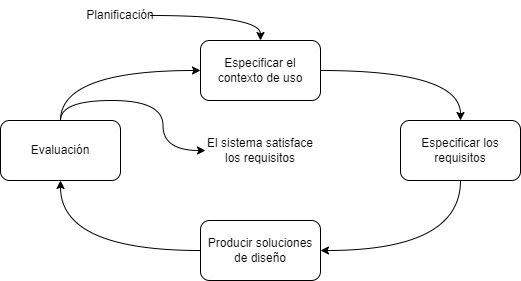
\includegraphics[width=0.70\textwidth]{Cap3/Figuras/DCU.jpg}
  \caption{Proceso del Diseño Centrado en el Usuario. Bratten, Concretamente, Hassan y Ortega (2009).}
  \label{fig:33}
\end{figure}

Es importante mencionar que este proceso también sugiere un enfoque para resolver problemas estratégicamente para mejorar su utilidad, es decir, durante el proceso se analiza la capacidad del producto para resolver necesidades.

Para lograr recabar toda la información necesaria para conocer al usuario, así como detectar sus necesidades, es necesario involucrar la observación, investigación y análisis del usuario, además de conocer sus actividades, el entorno que percibe y el contexto en el que tomaría lugar el uso del producto.

% REFERENCIA
Para lograr los resultados más adecuados para el diseño centrado en el usuario, se recurre a guías que se denominan metodologías para el diseño centrado en el usuario. Bratten, Concretamente, Hassan y Ortega (2009), señalan que estas metodologías o técnicas tienen como objetivo conocer y comprender las necesidades de los usuarios, así como el comportamiento y limitaciones en casos reales en los que se usaría el sistema a partir de una interfaz. Con ello se pretende responder preguntas que ayudan a mejorar el diseño centrado en el usuario, tal que permitan determinar descripciones, procedimientos, ubicaciones, limitaciones y problemas que se pudieran presentar.

Para conocer cada una de las características y puntos mencionados anteriormente, se recurre a la aplicación de test o pruebas de un sistema a usuarios. Es importante tener en cuenta que estas pruebas pretenden evaluar el sistema y la usabilidad del diseño, mas no al usuario.

%------------------------------------------------------------
%	Técnicas del análisis del usuario
%------------------------------------------------------------

\section{Técnicas del análisis del usuario}
\label{TecnicasAnalisisCap3}

Las técnicas del análisis del usuario permiten formar herramientas que proveen información específica y relevante de diferentes aspectos de los usuarios a los que va dirigido un producto. Esta información puede incluir desde sus intereses personales, dificultades o frustraciones, emociones al usar un sistema o incluso identificar problemas que pueden ser atacados para facilitar la resolución de problemas en el sistema, producto o servicio desarrollado.

A continuación se describen dos técnicas del análisis del usuario, que permiten extraer información específica que es útil para el diseño del producto: Persona y Customer Journey Map.

%------------------------------------------------------------
%	Persona
%------------------------------------------------------------

\subsection{Persona}
\label{PersonaCap3}

La fundación de diseño de interacción, señala que la técnica conocida como Personas, consiste en crear personajes ficticios que cumplan con las características necesarias de los usuarios que podrían usar un producto o un servicio. Esta herramienta permite entender de mejor forma las necesidades, experiencias y comportamientos de los usuarios, lo cual provee información para mejorar el diseño de los productos.

Las herramientas resultantes de la técnica Personas, aportan un esquema de apoyo para el diseño de la experiencia de usuario, el cual genera empatía y acercamiento al mundo de los usuarios a través del producto diseñado. El objetivo principal de la técnica es definir de forma clara las necesidades identificadas en los usuarios, con el fin de establecer funcionalidades necesarias para implementar y aplicar en el producto final.

La fundación de diseño de interacción propone una serie de reglas para crear y diseñar de forma correcta un producto Persona que cumpla con su función adecuadamente. Estas reglas se mencionan a continuación:

\begin{enumerate}
  \item Recopilar la mayor cantidad de datos sobre los usuarios objetivos.
  \item Determinar las características que se comparten y difieren entre los usuarios.
  \item Desarrollar hipótesis resultantes de la investigación, considerando las cualidades y diferencias determinadas en el punto anterior.
  \item Confirmar que las partes interesadas estén de acuerdo con las hipótesis definidas en el punto anterior.
  \item Determinar la cantidad de personas involucradas para la creación del esquema Persona. Es importante concentrarse sólo en una persona para desarrollar el esquema.
  \item Nombrar y describir a cada persona en un esquema de una o dos páginas. Este apartado debe incluir la siguiente información:
  \begin{enumerate}[a)]
    \item Fotografía del usuario.
    \item Valores, intereses, educación, estilo de vida, necesidades, actitudes, deseos, limitaciones, metas y patrones de comportamiento del usuario.
    \item Detalles adicionales que hagan más reales los datos del esquema, con el fin de generar más empatía.
  \end{enumerate}
  \item Describir situaciones en las que el usuario podría usar el producto y colocarlo en contextos con problemas a superar.
  \item Incluir a todos los involucrados del proyecto para aceptar a la persona o aconsejar revisiones.
  \item Enviar los datos recopilados para usar en el producto.
  \item Desarrollar los escenarios en los que se podría usar el producto. Estos deben exponer de manera clara a la persona en los posibles casos de uso.
  \item Realizar ajustes continuos para agregar nuevas características o descartar personas obsoletas.
\end{enumerate}

Una vez que las personas involucradas en el proyecto entienden de forma más clara a los usuarios, es pertinente definir el límite de los detalles a considerar para aportar a un producto, con el fin de delimitar aquellas características que se ajusten a los diseños. La fundación de diseño de interacción señala que con esta información también se puede crear un prototipo con la recopilación de los datos más importantes, el cual debe incluir los siguientes puntos.

\begin{enumerate}
  \item Las características del usuario deben permanecer en contexto.
  \item Refleja de forma general el comportamiento, las actitudes, un conjunto de habilidades y motivaciones, así como los objetivos que tiene el usuario dentro del dominio del producto.
  \item Conocer el objetivo del usuario, lo que quiere resolver y los problemas que quiere abordar, así como las características que le ayudarían a resolver los problemas de mejor forma a como lo hace.
  \item Identificar e incluir los escenarios realistas que enfrenta el usuario, e imaginar cómo usarían el producto para lograr un objetivo particular.
  \item Ocupar un entorno coronado que muestre una rutina cotidiana del usuario.
  \item Identificar los aspectos de dificultar o frustración del usuario.
\end{enumerate}

A continuación se presenta un esquema final en la Figura \ref{fig:34}, resultado de todos los puntos y aspectos mencionados anteriormente. En el siguiente ejemplo, se tiene una aplicación que permite buscar, controlar y reproducir música, la cual tiene el usuario llamado Rebecca, que representa a usuarios de 26 años que usan algunas aplicaciones como Spotify para reproducir música. A través del usuario Rebecca, se puede observar como la aplicación ayuda a usuarios con el mismo perfil o similar en su día a día. Imaginemos que Rebecca gusta de escuchar música de calidad, compartir música con amigos, familiares y tiene un mecanismo de clasificación de música de diferentes géneros. Su objetivo es reproducir música de calidad de forma rápida, cómoda y fácil.

\begin{figure}[H]
% \begin{figure}
  \centering
  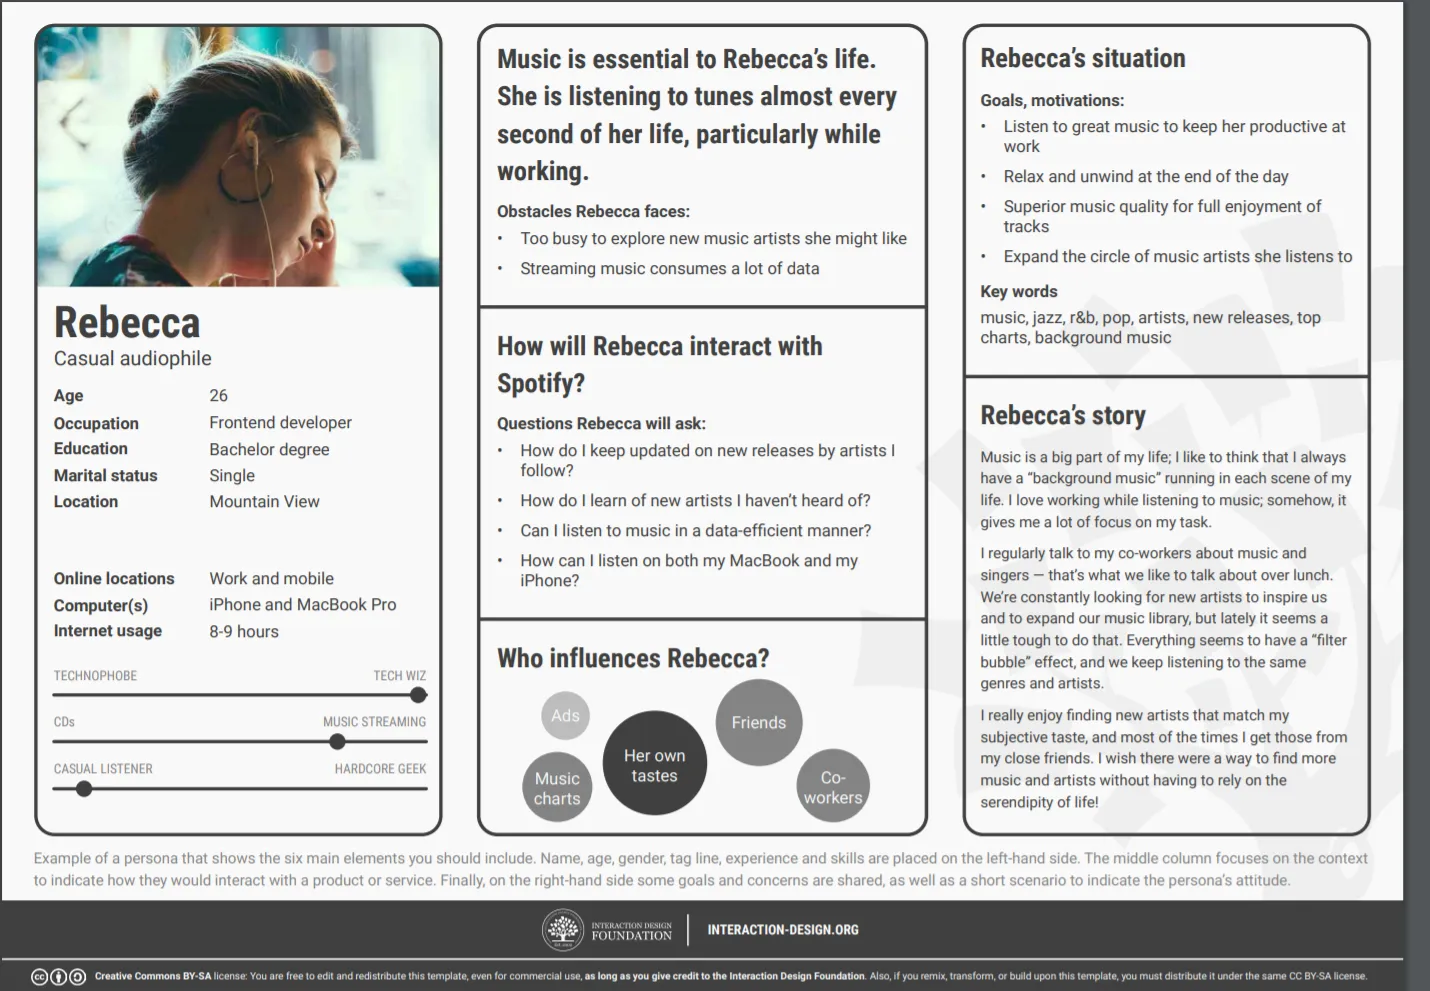
\includegraphics[width=0.70\textwidth]{Cap3/Figuras/EjemploPersona.jpg}
  \caption{Ejemplo de Persona. Interaction Design Foundation (2022a).}
  \label{fig:34}
\end{figure}

%------------------------------------------------------------
%	Customer Journey Map
%------------------------------------------------------------

\subsection{Customer Journey Map}
\label{CustomerJourneyMapCap3}

% REFERENCIA
Komninos y Briggs (2022) señalan que un Customer Journey Map es una herramienta que examina la historia de cómo un usuario se relaciona con un producto o servicio a lo largo del tiempo. Esta herramienta sirve para generalizar una idea del viaje que podría tomar un usuario con un producto, lo cual proporciona información sobre las interacciones en cada punto de un sistema, así como la capacidad de mejora en la interacción del sistema con un usuario en iteraciones futuras.

Por otro lado, ayudan a facilitar la comprensión de cómo se debe tratar de forma general a los usuarios en diferentes contextos y puntos del sistema para realizar una tarea. Además permite determinar una organización detallada de cómo los usuarios progresan en el uso del producto para lograr sus objetivos o resolver subtareas, con el fin de determinar un proceso de comunicación amplio y centrado en el usuario.

Un Customer Journey Map también provee información sobre los sentimientos que percibe un usuario en cada una de las etapas del uso de un producto. Permite explorar lo que los usuarios sienten, ven, oyen, hacen, plantean y piensan.

% REFERENCIA
Komninos y Briggs (2022) recomiendan preparar ciertos requisitos antes de comenzar con la elaboración de un Customer Journey Map. Se recomiendan los siguientes puntos.

\begin{itemize}
  \item Tener definido un esquema Persona.
  \item Definir una escala de tiempos. Es decir, tener un aproximado de la duración que tardará cada proceso del Customer Journey Map.
  \item Definir claramente los puntos de interacción con el usuario, para saber la tarea que realizan y cómo la realizan.
  \item Comprender e identificar los canales en los que se producen las acciones. Estos son los lugares donde los usuarios interactúan con un producto.
  \item Identificar los distractores o actores que puedan alterar la experiencia del usuario, tales como familia, amigos, ruido, entre otros.
  \item Determinar un plan de lo que se conoce como $"$momentos de la verdad$"$, los cuales son interacciones que causan sentimientos positivos en puntos de interacción donde existe frustración.
\end{itemize}

Es importante mencionar que los puntos anteriores no se consideran como requisitos para comenzar con la creación de un Customer Journey Map, sin embargo, podrían ser muy útiles para que el proceso de creación sea más claro y detallado. La fundación de interacción de diseño propone los siguientes puntos para la creación de un Customer Journey Map.

\begin{itemize}
  \item Identificar las metas y objetivos que se desean alcanzar con el producto, así como identificar las necesidades de los usuarios que se pretenden satisfacer.
  \item Considerar la investigación sobre los usuarios para determinar su interacción durante cada paso del Customer Journey Map. En caso de no tener una investigación adecuada que provea información de los usuarios a los que un producto va dirigido, es necesario determinar una forma en que se lleve a cabo.
  \item Definir los puntos de contacto e interacción del producto. Un punto de contacto es un paso en el recorrido en el que un usuario interactúa con un producto. Los puntos de contacto se traducen a las acciones que se tienen que realizar para lograr un objetivo desde un punto inicial.
  \item Crear un mapa de empatía, el cual examina cómo se siente un usuario durante cada punto de contacto. En particular se examina cómo se siente y piensa el usuario, para saber cómo reacciona a partir de lo que dirá, hará, escuchará, entre otros comportamientos.
  \item Construir un diagrama de afinidad. Se recomienda aplicar una lluvia de ideas sobre cada concepto y relacionarlos con los sentimientos y los datos recopilados en los puntos anteriores. Para ello, se agrupan los resultados en categorías. En esta etapa también se eliminan conceptos que parecen no tener impacto en la experiencia del usuario con cada punto de contacto.
  \item Dibujar el recorrido del usuario, en el que se reúnan los datos recopilados en forma de línea de tiempo. Este recorrido tiene la finalidad de mostrar el movimiento de un usuario a por cada uno de los puntos de contacto y canales a lo largo del viaje desde un punto de inicio. Este mapa incluye los datos incluidos en el mapa de empatía y diagrama de afinidad.
  \item Convertir el resultado anterior en una herramienta útil, en la cual se sigue refinando y actualizando el contenido. Este resultado debe ser claro y atractivo para las personas interesadas en la información.
  \item Dar a conocer el Customer Journey Map en todos los integrantes del equipo que harán uso de la información, con el fin de poner en uso los resultados analizados.
\end{itemize}

Es importante mencionar que este puede tomar el formato que más se acomode a las necesidades requeridas, sin embargo, se presenta un ejemplo a continuación de un Customer Journey Map en la Figura \ref{fig:35} con el formato más usado para representar los resultados.

\begin{figure}[H]
% \begin{figure}
  \centering
  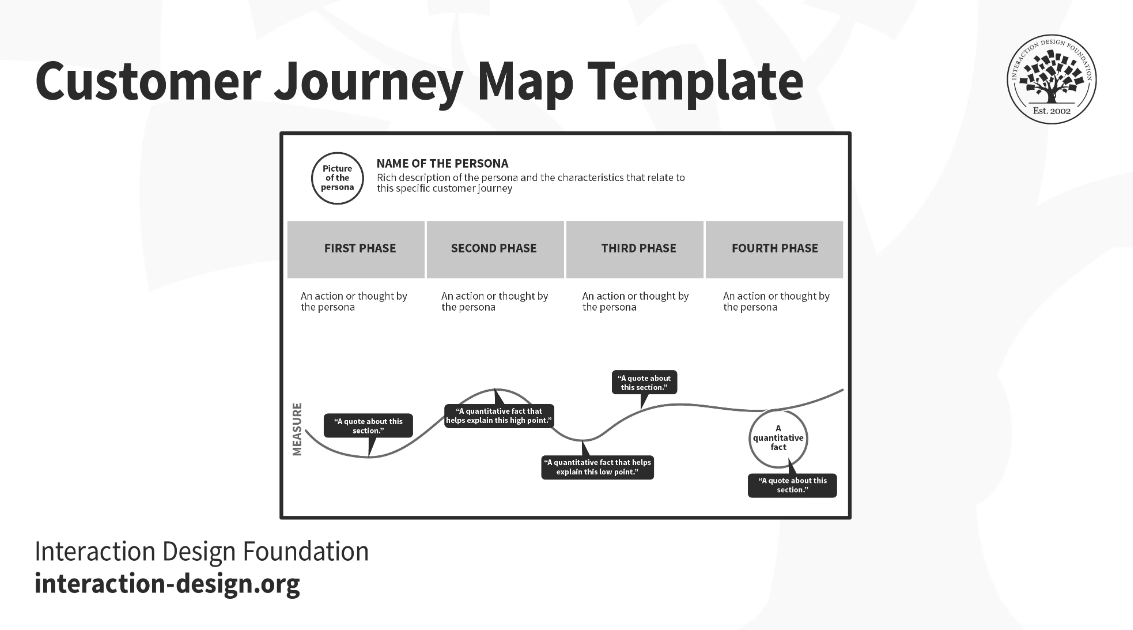
\includegraphics[width=0.70\textwidth]{Cap3/Figuras/CustomerJourneyMapEjemplo.png}
  \caption{Ejemplo de Customer Journey Map (Interaction Design Foundation, 2020b).}
  \label{fig:35}
\end{figure}

En esta representación, el Customer Journey Map se divide en diferentes secciones. En la zona superior se muestran los datos generales del usuario, seguido de las etapas o también llamados puntos de contacto. En cada punto se agrega la información relacionada a los pensamientos, acciones y experiencias del usuario, los cuales están basados en la información recolectada, tal como el mapa de empatía o el diagrama de afinidad, entre otros. Finalmente se muestran los canales de cada punto de contacto, que son aquellos detalles de cómo se lleva a cabo la interacción, tal como por correo electrónico, usando un sitio web, etcétera.

Esta herramienta permite una comprensión detallada de la experiencia de un usuario en cada punto de un producto, a partir de un enfoque basado en $"$un día en la vida de un usuario$"$ que genera información útil de cómo es el punto de vista de un usuario con un sistema en un ambiente cotidiano. Esto da como resultado, la oportunidad de llevar la empatía a un diseño que se adopte de mejor forma a las necesidades de un usuario, así como eliminar o evitar de forma eficiente los puntos de frustración tanto como sea posible.

%------------------------------------------------------------
%	Evaluaciones con el usuario
%------------------------------------------------------------

\section{Evaluaciones con el usuario}
\label{EvaluacionesCap3}

Las evaluaciones con el usuario consisten en una serie de pruebas, en las que se solicita al usuario realizar ciertas actividades, comisionadas por una persona denominada como evaluador. Con estas evaluaciones, el o los diseñadores pueden identificar posibles problemas que difícilmente estos podrían encontrar por la gran familiaridad y el manejo de un proyecto. Con las observaciones encontradas por los diseñadores y el evaluador, se logra identificar la descripción, procedimientos, limitaciones y problemas en el diseño.

%------------------------------------------------------------
%	Usabilidad
%------------------------------------------------------------

\subsection{Usabilidad}
\label{UsabilidadCap3}

% REFERENCIA
Hassan (2002) señala que la usabilidad es la disciplina encargada de estudiar la forma de diseñar sistemas, con el fin de brindar a los usuarios una forma fácil, cómoda e intuitiva de interactuar con un sistema, un producto o un servicio.

% REFERENCIA
El principal objetivo de la usabilidad, es lograr que el producto final sea usable para los usuarios. Hassan (2002) propone que una buena forma de lograr el objetivo, es crear un diseño del sistema centrado en el usuario. A diferencia del diseño centrado en la tecnología, que se enfoca en la forma más sencilla y cómoda de implementar un sistema, el diseño centrado en el usuario se enfoca en resolver las necesidades de los usuarios objetivos de forma fácil, por medio de estudios de los usuarios, creando herramientas, en las que se encuentran la técnica Persona y el Customer Journey Map, mencionados anteriormente, entre otros que puedan extraer información útil y relevante para mejorar la experiencia para el usuario.

Existe un concepto que se encuentra estrechamente relacionado a la usabilidad, denominado $"$findability$"$, que se refiere a la posibilidad de que cierta información sea encontrada o recuperada de forma accesible. La $"$findability$"$ proporciona la intervención de motores e índices de búsqueda, que facilita el proceso de recuperación o búsqueda de información. La usabilidad se apoya de diferentes conceptos para mejorar el proceso de diseño, entre ellos la $"$findability$"$, con el fin de permitir una navegación más sencilla e intuitiva dentro del ambiente de un sistema para disponer de los datos requeridos de forma sencilla.

Otro concepto del que se apoya la usabilidad, es la accesibilidad, que tiene como objetivo proveer diferentes formas de interacción para que los usuarios con alguna discapacidad puedan tener una forma de interacción para acceder a los contenidos del sistema. Así mismo, la accesibilidad propone que el contenido de un sistema debe poder proveer su contenido en diferentes tipos de dispositivos sin importar el hardware o software.

Finalmente, la usabilidad se apoya también en la utilidad, que se refiere a la cualidad de cubrir satisfactoriamente las necesidades del usuario.

% REFERENCIA
Es así como la usabilidad se convierte en la aplicación de un conjunto de conceptos para desarrollar un producto interactivo intuitivo y fácil de usar. Hassan y Ortega (2009c) mencionan algunos componentes principales que brinda la usabilidad.

\begin{itemize}
  \item \textbf{Facilidad de Aprendizaje.} Se refiere a la facilidad que muestran los usuarios para llevar a cabo las tareas para lograr sus objetivos por primera vez en el sistema.
  \item \textbf{Eficiencia.} En relación al tiempo se tardan los usuarios en realizar las tareas una vez que ya han aprendido el funcionamiento del sistema. Entre menor sea el tiempo que se tardan realizando las tareas, más eficiente es el sistema.
  \item \textbf{Cualidad de ser recordado.} Se refiere al tiempo en que los usuarios recuerdan o adquieren conocimiento del producto después de no ser usado por un periodo de tiempo. Entre menor sea el tiempo para recordar, mejor será la cualidad de ser recordado.
  \item \textbf{Eficacia.} La eficacia se determina por los errores que comete el usuario en el sistema. Se considera la gravedad de los errores y la rapidez en la que deshacen las consecuencias de haberlos cometido. Entre menos errores se comentan y entre menor sea el tiempo de su solución, más eficiente será el sistema.
  \item \textbf{Satisfacción.} Es la decisión del usuario como resultado de su experiencia en la interacción con el sistema. Se determina lo agradable y sencillo que le pareció para lograr satisfacción al usar el sistema.
\end{itemize}

Por otro lado, es importante contar con un proceso de evaluación de usabilidad, para corroborar que la implementación cumpla con los objetivos que ofrece la usabilidad. Además, las evaluaciones son útiles para encontrar errores o comportamientos que podrían resultar confusos para los usuarios.

Existen diferentes tipos de evaluación que apoyan la valoración de usabilidad de un producto, tal como los cuestionarios, que consisten en responder una serie de preguntas bien definidas y elaboradas por expertos, o los test de usabilidad, que consisten en realizar pruebas con usuarios usando el sistema o producto y analizando su comportamiento e interacción.

%------------------------------------------------------------
%	Cuestionario de usabilidad (SUS)
%------------------------------------------------------------

\subsection{Cuestionario de usabilidad (SUS)}
\label{SUSCap3}

% REFERENCIA
Existen diferentes formas de realizar la evaluación de la usabilidad de un sistema, entre las que se encuentra la escala de usabilidad del sistema o SUS (System Usability Scale). Brooke (1995), señala que SUS es una herramienta creada por John Brooke en 1986, la cual permite medir la usabilidad de un sistema a partir de un cuestionario con diez reactivos, cada uno de los cuales tiene cinco opciones de respuesta que van desde $"$Fuertemente de acuerdo$"$ a $"$Fuertemente desacuerdo$"$.

SUS provee una serie de beneficios y puntos a considerar durante su aplicación. Algunos de los beneficios que ofrece esta herramienta son los siguientes.

\begin{itemize}
  \item Es una herramienta que permite administrar a los participantes fácilmente.
  \item Se puede aplicar a una cantidad pequeña de muestras con resultados fiables.
  \item Puede determinar fácilmente si un sistema es utilizable o inutilizable.
\end{itemize}

% REFERENCIA
Por otro lado, Brooke (1995) propone las siguientes consideraciones al usar la herramienta.

\begin{itemize}
  \item El sistema de puntuación para determinar la usabilidad del sistema puede resultar complejo.
  \item Cuando se obtiene el resultado final de usabilidad en una escala de 0 a 100, no se debe interpretar como un valor que define un porcentaje.
  \item SUS es una herramienta que permite clasificar la facilidad de uso, la aplicación o el entorno, pero no funge el rol de ser un diagnóstico del sistema.
\end{itemize}

% REFERENCIA
Por lo que se refiere a la evaluación, Brooke (1995) sugiere calificar y evaluar con diez reactivos. A continuación, se proponen los siguientes reactivos, que deben ser adaptados al sistema o particularidades que son útiles para formar parte de los resultados.

\begin{enumerate}
  \item Creo que me gustaría usar este sistema con frecuencia.
  \item Encontré el sistema innecesariamente complejo.
  \item Pienso que el sistema es fácil de usar.
  \item Creo que necesitaré el apoyo de un técnico para poder utilizar este sistema.
  \item Encontré que las diversas funciones de este sistema estaban bien integradas.
  \item Pienso que había demasiada inconsistencia en este sistema.
  \item Me imagino que la mayoría de la gente aprenderá a usar este sistema muy rápidamente.
  \item Encuentro el sistema muy engorroso de usar.
  \item Me sentí muy confiado usando el sistema.
  \item Necesito aprender muchas cosas antes de poder ponerme en marcha con este sistema.
\end{enumerate}

Nótese con atención que cada reactivo está estructurado de forma que los reactivos impares (1, 3, 5, 7, 9) se refieren a enunciados con carácter positivo, mientras que los reactivos pares (2, 4, 6, 8, 10) son enunciados negativos.

Para las preguntas con carácter o actitud positiva, se toma el resultado de los usuarios en la escala de 1-5 y se le resta una unidad. En cambio, para las preguntas de carácter negativo, se le resta el resultado del usuario a un valor fijo de 5.

Una vez que todos los usuarios han respondido el cuestionario, se deben interpretar los resultados a partir de un proceso específico propuesto por SUS. El proceso de interpretación de resultados consiste en convertir las puntuaciones de los participantes en un número nuevo.

Los valores modificados anteriormente se suman para cada tipo de pregunta, se suma por cada uno de los usuarios que respondieron el cuestionario. El valor total de la suma se multiplica por 2.5. Finalmente, se obtiene el promedio de la suma del valor total de cada usuario que se obtuvo anteriormente.

El valor resultante se asocia a una puntuación definida por SUS, mostrada a continuación.

\begin{itemize}
  \item Si el valor es menor o igual a 25 puntos, entonces el sistema se considera pésimo.
  \item Si el valor se encuentra entre el rango de 26-39 puntos, entonces el sistema se considera pobre.
  \item Si el valor se encuentra entre el rango de 40-51 puntos, entonces el sistema se considera suficiente.
  \item Si el valor se encuentra entre el rango de 52-73 puntos, entonces el sistema se considera bueno.
  \item Si el valor se encuentra entre el rango de 74-85 puntos, entonces el sistema se considera excelente.
  \item Si el valor es mayor de 86 puntos, entonces el sistema se considera extremadamente bueno.
\end{itemize}

Estas escalas se muestran en la Figura \ref{fig:36}.

\begin{figure}[H]
% \begin{figure}
  \centering
  \includegraphics[width=0.70\textwidth]{Cap3/Figuras/Clasificación de calificaciones de puntajes SUS.jpg}
  \caption{Clasificación de calificaciones de puntajes SUS. Brooke, J. (2013).}
  \label{fig:36}
\end{figure}

%------------------------------------------------------------
%	Proceso de evaluación del grupo ESIE
%------------------------------------------------------------

\subsection{Proceso de evaluación del grupo ESIE}
\label{ESIECap3}

El grupo ESIE ha desarrollado un proceso estándar que permite evaluar la usabilidad. Este proceso propone una serie de herramientas, pasos y participantes asignados a un rol específico que tienen un papel fundamental durante el proceso.

Las herramientas sirven como apoyo para recabar información de un proceso de evaluación. En particular, para este proyecto se utilizaron las siguientes herramientas.

\begin{itemize}
  \item \textbf{Hipótesis de la prueba.} Es un documento que toma la información de seis puntos relevantes.
  \begin{itemize}
    \item Estado de la interacción. Es el punto o estado en que se encuentra el sistema antes de realizar alguna tarea específica en el sistema.
    \item Hipótesis. Es la suposición de lo que se espera en el comportamiento del usuario al realizar una actividad específica.
    \item Tarea. Corresponde a la solicitud que se indicará al usuario para realizar cierta tarea en el sistema. Esta debe ser concreta, directa, clara y sin palabras que infieran cómo resolver la tarea.
    \item Desarrollo de la tarea. Es la acción que se debe realizar en el sistema para cumplir la tarea solicitada. Esta información sólo la conoce el evaluador durante la evaluación, más no el usuario.
    \item Tiempo estimado. Es el tiempo aproximado que se estima para poder realizar la tarea.
    \item Resultado. Son las anotaciones que determinan si la tarea se resolvió satisfactoriamente, dependiendo de la hipótesis propuesta. Además se pueden incluir comentarios extra como dificultades o imprevistos al realizar la tarea.
  \end{itemize}
  Esta herramienta puede dar paso a la creación del documento de actividades de la prueba.
  \item \textbf{Cuestionario de entrada.} Es un cuestionario con reactivos en los que se solicita información del usuario, tal como su edad, el tipo de herramientas y dispositivos que utiliza, así como sus interés y frecuencia con la que usa las herramientas. Estas preguntas van enfocadas a saber información que este relacionada al proyecto que se evalúa.
  \item \textbf{Protocolo de bienvenida.} Es un documento que consiste en la presentación de objetivos de la evaluación. Así mismo, se presenta el monitor y presenta las funcionalidades generales del sistema. Se pone especial detalle en expresar que la evaluación es sobre la usabilidad del sistema, más no del usuario en particular.
  \item \textbf{Actividades de la prueba.} Es un listado con todas las actividades que debe realizar el usuario. Esta herramienta es un apoyo para el encargado de la evaluación.
  \item \textbf{Cuestionario de usabilidad.} Es un cuestionario que contiene reactivos específicos para determinar la usabilidad del sistema. En particular, para este proyecto se usa el cuestionario de usabilidad SUS, desarrollado en la sección \ref{SUSCap3}.
  \item \textbf{Cuestionario de percepción subjetiva.} Es un cuestionario que contiene reactivos de tipo escala, en la que se identifican particularidades de la interfaz de usuario del sistema. La escala que toman los reactivos van de uno a nueve, en donde uno corresponde a escalas no favorables y nueve a percepciones satisfactorias y positivas.
\end{itemize}

Por otra parte, el proceso de evaluación del grupo ESIE propone un conjunto de roles con tareas específicas a desarrollar durante la evaluación.

\begin{itemize}
  \item \textbf{Expertos.} Son personas encargadas del diseño de los instrumentos, mencionadas en la sección anterior, y el análisis de la información de los resultados de las pruebas.
  \item \textbf{Monitor.} Es la persona encargada de dirigir al usuario con las actividades que debe realizar como forma de guía.
  \item \textbf{Observador.} Es la persona encargada de supervisar la evaluación. Verifica que no se omita ninguna de las actividades, así como realizar un respaldo de la evaluación por medio de videos, fotografías o escritos en notas.
  \item \textbf{Anfitriones.} Son las personas encargadas de tener un control y coordinación para verificar que los usuarios respondan completamente y tener organización de los resultados de cada usuario.
\end{itemize}

El proceso de evaluación del grupo ESIE propone tres fases para realizar la evaluación de usabilidad, mismas que se mencionan a continuación:

\begin{itemize}
  \item \textbf{Primera fase.} El anfitrión o anfitriones dan la bienvenida a los usuarios y solicita que llenen los documentos de perfil de usuario, el cual consta de información como edad, escolaridad, aplicaciones que usa, dispositivos que maneja, la frecuencia con las que se utilizan, entre otros. Es importante recalcar, que en esta fase se hace la solicitud de consentimiento de los usuarios para poder registrar la evaluación por medio de videos y fotografías, con el fin de usarse como apoyo al análisis de la evaluación.
  \item \textbf{Segunda fase.} En esta fase, se provee al usuario de todas las herramientas necesarias para poder manejar el sistema, dentro de un espacio sin distracciones. En este punto, el monitor toma el mando en el proceso de evaluación, el cual estará cerca del usuario o usuarios, quienes tienen frente a ellos el dispositivo con la aplicación. Es importante localizar al monitor en un espacio que no obstruya las cámaras, micrófonos o cualquier otro dispositivo de registro.
  
  El papel del monitor consiste primeramente en leer una carta de bienvenida, la cual especifica las reglas a seguir durante la evaluación, así como los objetivos, motivos y datos extra que se esperan obtener como resultado de la evaluación. Posterior al término de la lectura de la carta de bienvenida, se crea un espacio de dudas, en la que se pregunta a los usuarios si hay algún punto que no sea claro. En caso de haber dudas, se responde a ellas, sin dar información de cómo realizar las actividades, en caso contrario, se procede al siguiente paso de esta fase.
  
  El monitor comienza a leer una serie de actividades en voz alta, el cual se conoce como guión de actividades. Las actividades deben ser completadas por los usuarios paso a paso como lo sugiere el monitor en el momento en que se sugiera. Estas actividades contienen todas las funcionalidades de una aplicación, por lo que se orienta al usuario a realizar todos las tareas que haría un usuario final.
  
  Mientras todo este proceso transcurre, el observador puede tomar notas de información que considere relevante para el análisis, tal como las reacciones al realizar alguna tarea o indagar en una funcionalidad en la aplicación. Cada vez que se termina una actividad, el monitor marca el apartado designado a esta actividad como completada y procede a leer la siguiente actividad. Es importante mencionar que una actividad no se puede dar como concluida y pasar a la siguiente si no se ha completado, sin embargo, sí puede dar sugerencias de apoyo después de cierto tiempo. En cada actividad, se coloca un registro del tiempo en que el usuario tardó en realizar la tarea.
  \item \textbf{Tercera fase.} Se solicita a los usuarios que respondan los cuestionarios de usabilidad y algunos otros cuestionarios extra que se consideren oportunos para extraer información útil para el análisis, tal como un cuestionario de percepción. Estos cuestionarios pueden contener una sección de comentarios adicionales que pudieran dejar los usuarios. Finalmente se agradece a los usuarios por su participación y con ello concluye el proceso de evaluación.
\end{itemize}

% REFERENCIA
Antes de realizar las pruebas, es primordial considerar una serie de cuestiones para obtener la información más útil posible para los análisis. Entre estos puntos, se encuentra la buena selección de participantes. El reclutamiento de un participante debe asegurar que cumple un perfil acorde con los usuarios reales que usarán el sistema. Kuniavsky (2003) señala que hay tres pasos a seguir para el reclutamiento de los participantes.

\begin{itemize}
  \item Determinar la audiencia del sistema o interfaz a evaluar.
  \item Encontrar participantes que representen la audiencia a la que está dirigido el sistema.
  \item Convencer a los usuarios a participar en la prueba.
\end{itemize}

% REFERENCIA
Una vez cumplidos los tres pasos anteriores, se procede a aplicar las pruebas a todos los participantes por separado o en conjunto en caso de así requerirse. Kuniavsky (2003) propone algunos requisitos que deben cumplir las tareas encomendadas por el evaluador.

\begin{itemize}
  \item \textbf{Ser razonables.} Solicitar tareas que un usuario real realizaría en el sistema.
  \item \textbf{Estar descritas en términos de objetivos finales.} La tarea debe estar contextualizada en una motivación mayor.
  \item \textbf{Ser específicas.} La tarea debe describir objetivos concretos.
  \item \textbf{Ser factibles.} Se evalúa el diseño y usabilidad a partir de los usuarios, pero nunca se evalúa a los usuarios o su manejo sobre el sistema.
  \item \textbf{Duración razonable.} Para tareas que requieren demasiado tiempo, se recomienda descomponer la tarea en subtareas.
\end{itemize}

Así mismo, estas pruebas pretenden encontrar los puntos específicos en los que el usuario se equivoca o se detiene al realizar alguna tarea solicitada, así como tratar de entender cómo es que surgieron esos problemas a partir de la observación del participante.

Por lo general, al final de la prueba se ofrece algún tipo de recompensa como agradecimiento a la participación en las pruebas. Una vez recolectados los datos se procede a analizar los resultados, con el fin de encontrar mejoras en el diseño, siguiendo así el ciclo del diseño centrado en el usuario mostrado en la Figura \ref{fig:33}.

Como se mencionó anteriormente, el diseño centrado en el usuario es un proceso iterativo, en el que cada versión de la interfaz corresponde a una iteración del proceso. Es por ello que las evaluaciones realizadas a los participantes, los resultados y la planificación de mejoras respecto a los análisis de las pruebas no reflejan la finalización del diseño de la interfaz, ya que posiblemente, esta pueda estar sujeta a nuevos cambios. Es por ello que el diseño centrado en el usuario provee un mecanismo de extensión al diseño de la interfaz.

%------------------------------------------------------------
%	Resumen
%------------------------------------------------------------

\section{Resumen}
\label{ResumenCap3}

En este capítulo se define una interfaz de usuario como un medio de interacción entre un sistema interactivo y un usuario. Se considera un conjunto de guías y principios para el diseño de la interfaz, así como algunas características provenientes de las teorías micro-HCI, que son aplicadas para la evaluación y el mejoramiento del diseño.
Posteriormente se definen las características y ventajas principales de diferentes tipos de interfaces, conocidas como interfaces multimodales o inteligentes. En particular, se pone especial énfasis en las características de las interfaces basadas en voz, tal como el procesamiento del sonido. A partir de esta información, se introducen los dispositivos basados en voz, tal como Alexa, Google Home, Google Assistant, Siri, entre otros, se presentan ventajas, desventajas y usos más frecuentes en la actualidad por los usuarios.

Finalmente, se presenta de forma teórica el Diseño Centrado en el Usuario (USD) y el proceso que sigue para el diseño de interfaces de un sistema. Como complemento, se mencionan algunas herramientas útiles para el proceso de diseño, que tienen el propósito de obtener información relevante sobre las necesidades y propósitos del usuario. Se estudian herramientas como la técnica Persona y el Customer Journey Map. Con el fin de evaluar la usabilidad del sistema, se presenta el concepto de usabilidad y una forma de evaluarla en un sistema por medio del cuestionario de usabilidad SUS y el proceso de evaluación del grupo ESIE.



%------------------------------------------------------------
%	CAPÍTULO IV
%------------------------------------------------------------

%------------------------------------------------------------
%	CAPITULO I
%------------------------------------------------------------

\chapter{Desarrollo de la skill}
\label{capIV}

El Buscador Gavilán, es una skill basada en reconocimiento de voz que tiene como objetivo mejorar el proceso de investigación y búsqueda de información por medio de una metodología formal de búsqueda, llamada Modelo Gavilán, detallado en el capítulo \ref{capII} del presente trabajo.

Por otra parte, el diseño de la skill toma bases teóricas del diseño de interfaces de usuario, ajustadas para las interfaces basadas en voz, tal como guías y principios mencionados en el capítulo \ref{capIII}. Algunas guías sobresalientes utilizadas son las siguientes:

\begin{itemize}
  \item Navegación en la interfaz
  \item Facilidad de entrada de datos
  \item Manipulación directa
  \item Lenguaje natural
\end{itemize}

También se consideran algunos principios de las ocho reglas de oro del diseño de interfaces, mostradas a continuación:

\begin{itemize}
  \item Usabilidad universal
  \item Comentarios o respuestas informativas
  \item Diálogos para término de acciones
  \item Prevención de errores
  \item Fácil retroceso de acciones
  \item Reducción de carga de memoria a corto plazo
\end{itemize}

Para el desarrollo del diseño de la skill, se toma como base una metodología basada en el diseño centrado en el usuario, la cual consiste en diseñar un sistema orientado a satisfacer las necesidades de los usuarios que harán uso de un producto o servicio. El diseño centrado en el usuario considera un proceso dividido en cuatro partes.

\begin{itemize}
  \item \textbf{Especificar el contexto de uso.} Para conocer de forma más cercana a los usuarios, se realizó una investigación del proceso de búsqueda de información con alumnos de licenciatura, con el fin de conocer la forma en que habitualmente realizan una investigación.
  \item \textbf{Especificar los requisitos.} Con el fin de identificar las necesidades del usuario, se desarrollaron herramientas para conocer la forma en las que se pueden satisfacer. En esta etapa se desarrollaron dos modelos para la técnica Persona, uno para un alumno de preparatoria y otro para un alumno de licenciatura, en los que se plantean sus intereses, objetivos, experiencias, entre otros.
  \item \textbf{Producir soluciones de diseño.} Con la información anterior, se presentó una serie de posibles soluciones por medio de un Customer Journey Map, en el que se realizaron ajustes e identificaron puntos de provecho para la implementación de la skill. Por otra parte, se crearon algunas propuestas para el diseño de la navegación por el sistema, en la que se agregaron mejoras hasta llegar a una versión estable para la implementación.  
  \item \textbf{Evaluación.} Con el fin de evaluar de forma precisa la usabilidad del sistema, se contó con cinco usuarios, con los cuales se aplicaron las pruebas basadas en el proceso de evaluación del grupo ESIE.
\end{itemize}

Dados los resultados obtenidos de todo el proceso de diseño, se logró una versión estable para su implementación, cuyo código se encuentra en un servicio de Amazon para el diseño de skills llamado Alexa Developer Console.

%------------------------------------------------------------
%	Alexa Amazon
%------------------------------------------------------------

\section{Alexa Amazon}
\label{AlexacapIV}

% REFERENCIA
Amazon (2022a), señala que Alexa es el servicio de voz de la compañía Amazon, disponible para los dispositivos de Amazon, tales como Amazon Echo, Echo Dot, Echo Pop y Echo Show, así como dispositivos terciarios con Alexa integrada. Por medio del servicio de Alexa, se crean capacidades y habilidades más personalizadas para los usuarios, llamadas skills. Alexa es un servicio que funciona por el reconocimiento por voz, de tal forma que cuando un usuario emite algún sonido o comando por voz, Alexa procesa la entrada y da una respuesta acorde a la información solicitada.

% REFERENCIA
Amazon (2022b) señala que el servicio Alexa Voice Service (AVS) provee todas las herramientas para poder integrar de forma correcta el servicio de reconocimiento por voz de Amazon. La documentación del servicio AVS provee los documentos para el desarrollo e identificación de requerimientos del producto, así como guías especializadas para desarrolladores.

Cabe recalcar que existe una gran diferencia entre los servicios de Alexa y Alexa Voice Service. Alexa es un servicio que se encarga de dar mantenimiento y función a los dispositivos Amazon Echo, mientras que AVS es un servicio enfocado a fabricantes de dispositivos comerciales. Entre estos fabricantes, se encuentran aquellos que utilizan AVS para incorporar Alexa en diferentes tipos de dispositivos, tales como altavoces, auriculares, computadoras, televisores, vehículos, entre otros dispositivos categorizados como inteligentes.

% REFERENCIA
AVS es un servicio que se puede apoyar de algunas herramientas que provee el equipo de desarrollo de Amazon (2022b), tales como las siguientes:

\begin{itemize}
  \item Alexa Built-in Product (ABI). Es una categoría de dispositivos que tienen integrado AVS, así como micrófonos, altavoces y un conjunto de funciones de Alexa para activación de palabras.
  \item AVS Device SDK. Son bibliotecas hechas en el lenguaje de programación C++, que utiliza las APIs de AVS. Estas bibliotecas facilitan y agilizan la integración de las características y funcionalidades de Alexa.
  \item APIs de Alexa. Son APIs para la implementación y automatización para directivas en la nube y eventos de un cliente.
\end{itemize}

% REFERENCIA
Alexa (2022b) recomienda considerar la respuesta de una serie de preguntas para el mejor diseño y desarrollo de un producto que utilice AVS. Entre estas preguntas se encuentran las siguientes:

\begin{enumerate}
  \item ¿Dónde será usado el producto por los clientes?
  \item ¿Este dispositivo agrega Alexa a espacios como el hogar, la oficina, habitaciones, vehículos o estará a dondequiera que vaya el cliente?
  \item ¿Que tipo de fuente de alimentación necesitará?
  \item ¿Accede a la nube de AVS por medio de Wifi o dependerá de Bluetooth y una aplicación móvil?
  \item ¿Cómo interactúa con los clientes?
  \item ¿Puede hablar con el dispositivo directamente o es necesario emparejarlo con otros dispositivos integrados a Alexa?
  \item ¿A qué distancia deben estar del dispositivo?
  \item ¿Cómo iniciarán la interacción?
  \item ¿Tendrá pantalla?
  \item ¿Qué pueden hacer los clientes con el producto?
\end{enumerate}

Es importante considerar estas características, ya que permiten tener una visión general del funcionamiento y casos de uso del producto o dispositivo final. La última pregunta del listado anterior, enfoca su contenido a la consideración de la incorporación de las funcionalidades con las que cuenta Alexa, tales como las que se muestran a continuación:

\begin{itemize}
  \item Activar a Alexa con la voz o el tacto, así como interrumpirla con la voz y el tacto.
  \item Permitir que transmita y controle música.
  \item Permitir la transmisión de sonido grupal en varias habitaciones de forma síncrona.
  \item Crear, detener y cancelar temporizaciones, alarmas y recordatorios.
  \item Recibir y eliminar notificaciones.
  \item Ver el contenido como tarjetas de visualización para dispositivos con pantalla.
  \item Emparejar dispositivos a través de Bluetooth.
  \item Mantener el contacto con llamadas, mensajes o anuncios.
  \item Presionar algún botón para hablar con Alexa, controlar el audio o alternar micrófonos.
\end{itemize}

%------------------------------------------------------------
%	Skills
%------------------------------------------------------------

\subsection{Skills}
\label{SkillscapIV}

% REFERENCIA
Alexa cuenta con diferentes funcionalidades, en las que se encuentran las skills. Amazon (2022c) define una skill como funcionalidades que permiten a los consumidores crear una experiencia más personalizada para realizar diferentes tareas. En pocas palabras, las skills son aplicaciones desarrolladas para el servicio de Alexa.

Las skills necesitan una palabra o comando para poder activarse. Un usuario puede activar una skill utilizando alguna palabra de activación, tal como $"$comienza$"$, $"$abre$"$ o $"$inicia$"$, seguido del nombre de la skill que se desea activar. Gracias al reconocimiento por voz y el procesamiento del lenguaje natural incorporado en Alexa, se reconoce el comando para que la skill solicitada se ejecute como un servicio en una plataforma en la nube. La forma de comunicación entre una petición y la nube se basa en el protocolo HTTPS, siendo la solicitud un verbo de tipo POST que contiene un payload de tipo JSON con el contenido necesario para dar respuesta al usuario por medio de Alexa.

En la Figura \ref{fig:41} se muestra el flujo de procesamiento para invocar una skill con Alexa.

\begin{figure}[H]
% \begin{figure}
  \centering
  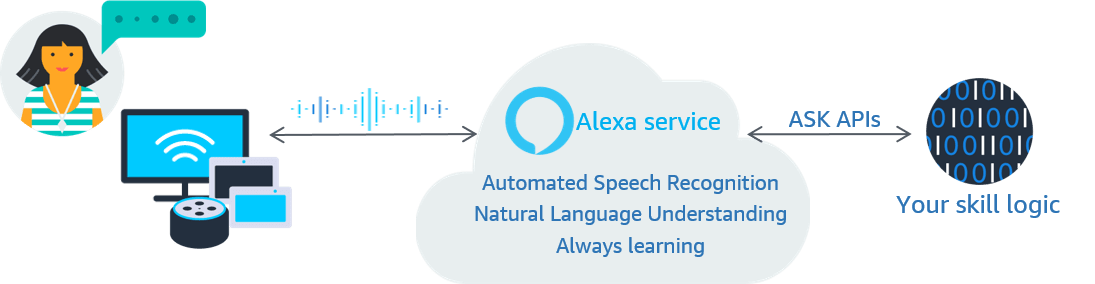
\includegraphics[width=0.70\textwidth]{Cap4/Figuras/ProcesoInvocacionSkill.png}
  \caption{Flujo de procesamiento de activación por voz para invocar una skill. Amazon (2022d).}
  \label{fig:41}
\end{figure}

%------------------------------------------------------------
%	Alexa Skills Kit (ASK)
%------------------------------------------------------------

\subsubsection{Alexa Skills Kit (ASK)}
\label{ASKcapIV}

% REFERENCIA
Amazon (2022c) señala que las skills se apoyan de un conjunto de herramientas para poder ser desarrolladas, llamado Skills Kit (ASK), que es el conjunto de herramientas, documentación, APIs, guías y ejemplos, que permiten el desarrollo y mantenimiento de las skills para Alexa de una forma sencilla y rápida.

Entre las herramientas que ofrece el ASK, se encuentran las siguientes:

\begin{itemize}
  \item La consola de desarrollo de Alexa, la cual contiene distintas opciones para respaldar el ciclo de vida de desarrollo.
  \item Bibliotecas que dan acceso a las funcionalidades de Alexa.
  \item Herramientas para poner a prueba la skill, tal como el simulador de funcionalidades de Alexa.
  \item Solucionador de problemas de reconocimiento de voz y procesamiento de lenguaje natural.
  \item Proporciona apartados para certificar y publicar la skill.
  \item Herramientas para administrar y monitorear las skills.
  \item Guía de diseño de Alexa para realizar las mejores prácticas de diseño de skills y modelos de interacción de voz personalizadas.
  \item Proporciona una biblioteca de intents para las expresiones más comunes.
  \item Documentación técnica, tutoriales y ejemplos de código para apoyar el proceso de creación de una skill.
\end{itemize}

%------------------------------------------------------------
%	Modelos de interacción de las skills
%------------------------------------------------------------

\subsubsection{Modelos de interacción de las skills}
\label{ModelosInteraccioncapIV}

% REFERENCIA
Amazon (2022e), señala que cada skill cuenta con un modelo de interacción de voz, en cual define las frases y palabras que un usuario puede decir mientras una skill está activada. De tal forma que cuando un usuario hace alguna solicitud, Alexa, con ayuda del ASK, toma como base el modelo de interacción de la skill para interpretar la solicitud y realizar la acción específica.

Alexa permite definir dos tipos de modelos de interacción de voz para las skills. Estos modelos se mencionan a continuación:

\begin{itemize}
  \item \textbf{Modelo de interacción de voz preconstruido.} El ASK determina el conjunto de palabras o frases que los usuarios dicen para invocar una skill. Las invocaciones de este modelo están enfocadas a solicitudes ya predefinidas.
  \item \textbf{Modelo de interacción de voz personalizado.} En este modelo el desarrollador diseña toda la interacción de voz, en la que se definen todas las formas en las que un usuario se puede comunicar y cómo la skill responde a cada tipo de solicitud definida en el modelo.
\end{itemize}

% REFERENCIAS
Para los dos tipos de modelo de interacción de voz, se debe definir el modelo sobre el que se va a basar la skill. Amazon (2022e) menciona algunos pasos recomendables para diseñar el modelo de interacción de una skill:

\begin{enumerate}
  \item Definir los intents que la skill puede reconocer. Los intents son acciones que un usuario puede realizar dentro de una skill. Se hablará a detalle más adelante.
  \item Definir los utterances, que son los enunciados o frases que los usuarios pueden decir para invocar un intent. Como un usuario puede solicitar una acción de diferentes formas, existe un mapeo de muchos enunciados a un intent.
  \item Definir el nombre que usará Alexa para identificar la skill. Este es el nombre con el que el usuario podrá formar el comando de activación de la skill.
  \item Opcionalmente, se pueden definir elementos visuales e interacciones táctiles para dispositivos que cuentan con una pantalla táctil con integración de Alexa.
  \item Definir la lógica de la skill para cumplir las intenciones personalizadas.
\end{enumerate}

Es importante recalcar que cualquier tipo de modelo de interacción por voz usa el mismo mecanismo de comunicación descrito en la Figura \ref{fig:41}.

%------------------------------------------------------------
%	Tipos de Skill
%------------------------------------------------------------

\subsubsection{Tipos de Skill}
\label{TiposSkillcapIV}

% REFERENCIA
Las skills que pueden ser desarrolladas tienen una clasificación definida por el ASK. Amazon (2022f) propone una clasificación que define el tipo de la skill según su modelo de interacción de voz, sus capacidades y características.

La Tabla \ref{tab:t41} describe los distintos tipos de skills, así como su enfoque.

\begin{table}[H]
  \begin{center}
    \begin{tabular}{ | p{4cm} | p{4cm} | p{8cm} | }
      \hline
      TIPO DE LA SKILL & MODELO DE VOZ & DESCRIPCIÓN  \\ \hline
      Automotive & Preconstruido y personalizado & Skills adaptadas a un automóvil. \\ \hline
      Business & Preconstruido & Skills que brindan acceso de voz a reuniones, calendarios comerciales, reserva de salas, etc. Este tipo también incluye skills enfocados a la hotelería y residencia. \\ \hline
      Cooking & Preconstruido & Skills para controlar y conectarse con aparatos de cocina. \\ \hline
      Custom & Personalizado & Skills con un modelo de interacción personalizado para la interacción con el usuario. \\ \hline
      Entertainment Device & Preconstruido & Skills que permiten controlar dispositivos inteligentes como televisores, altavoces, entre otros. \\ \hline
      Flash Briefing & Preconstruido & Skills que proporcionan información como noticias o contenido breve de Flash Briefing. \\ \hline
      Games & Personalizado & Skills enfocadas a la interacción con juegos manejados por voz. Estas skills se apoyan fuertemente de imágenes para dispositivos con pantalla. \\ \hline
      Knowledge & Knowledge & Skills que permite a los usuarios conocer información sobre cálculos de una organización sin invocar el nombre de la skill. \\ \hline
      List & Personalizado & Skills que permiten leer y actualizar las listas de un usuario de Alexa. \\ \hline
      Music, Radio, and Podcast & Preconstruido & Skills que permiten controlar audio transmitido a través de los dispositivos habilitados para Alexa. \\ \hline
      Networking and Wi-Fi & Preconstruido & Skills para modelar redes Wi-Fi domésticas. \\ \hline
      Smart Home & Preconstruido & Skills que permiten controlar los dispositivos domésticos inteligentes. \\ \hline
      Smart Home Energy & Preconstruido & Skills que permiten administrar el uso de energía de Alexa. \\ \hline
      Smart Home Security & Preconstruido & Skills que permiten controlar dispositivos de seguridad domésticos inteligentes, tales como cámaras, cerraduras, sensores de movimiento, entre otros. \\ \hline
      Video & Preconstruido & Skills que permiten controlar dispositivos de video, así como consumir video. \\ \hline
    \end{tabular}
    \caption{Tipos de Skill según su enfoque}
    \label{tab:t41}
  \end{center}
\end{table}

%------------------------------------------------------------
%	Flujo de desarrollo de una Skill
%------------------------------------------------------------

\subsubsection{Flujo de desarrollo de una Skill}
\label{FlujoSkillcapIV}

% REFERENCIA
Amazon (2022d) señala que el desarrollo de cualquier tipo de skill sigue un proceso de diseño, creación e implementación que se divide en cinco etapas.

\begin{enumerate}
  \item \textbf{Diseñar la skill.} Consiste en diseñar un modelo de interacción por voz de tal forma que la conversación sea natural y se base en un diseño centrado en el usuario. 
  \item \textbf{Construir la skill.} Esta etapa consiste en implementar el modelo de interacción de voz. Para los modelos de interacción personalizados, la skill se construye a partir de las herramientas que provee ASK y un entorno de desarrollo apropiado para el lenguaje de programación seleccionado para su implementación.
  \item \textbf{Probar la skill.} Las pruebas de la skill pueden hacerse fácilmente sin un dispositivo, utilizando el simulador de Alexa, que se encuentra incorporado en la consola de desarrollo de Alexa. En este simulador se pueden definir varias características, tales como los diferentes dispositivos y la interacción multimodal.
  \item \textbf{Certificar y publicar la skill.} Antes de que una skill sea publicada en la tienda de Skills de Alexa, se debe pasar por un proceso de certificación para asegurar que cumpla todos los requisitos de calidad, seguridad y políticas de Amazon. Si todas las pautas se cumplen, la skill estará disponible en la tienda de skills de Amazon para los usuarios de Alexa. 
  \item \textbf{Supervisar la skill.} Es posible monitorear el uso de la skill en vivo, así como ejecutar un análisis y consultar las ganancias en caso de haber. 
\end{enumerate}

Este proceso se sigue como en la Figura \ref{fig:42}.

\begin{figure}[H]
% \begin{figure}
  \centering
  \includegraphics[width=0.70\textwidth]{Cap4/Figuras/Flujo de creación de skill.jpg}
  \caption{Flujo de creación de una skill. Amazon (2022d).}
  \label{fig:42}
\end{figure}

%------------------------------------------------------------
%	Alexa Developer Console
%------------------------------------------------------------

\subsection{Alexa Developer Console}
\label{ADCcapIV}

La consola de desarrollo de Alexa es una herramienta que se encuentra contenida en el ASK. Su objetivo es brindar un control del flujo de creación de una skill.

La consola de desarrollo de Skills se divide en cinco secciones:

\begin{itemize}
  \item \textbf{Skills.} Listado de las skills desarrolladas en la cuenta de Amazon.
  \item \textbf{Ganancias.} Se muestran datos informativos sobre las ganancias generadas con las skills publicadas en la tienda de skills de Amazon.
  \item \textbf{Pagos.} Se muestra información de los pagos realizados durante un periodo.
  \item \textbf{Alojamiento.} En este apartado se presenta información relacionada al uso de algunos servicios de Amazon Web Services (AWS), tales como AWS Lambda, Amazon S3, Amazon DynamoDB, entre otros.
  \item \textbf{Configuraciones.} Se muestra información de administración del acceso a la skill, gestión de usuarios e id's.
\end{itemize}

Estas opciones se encuentran en la presentación de la consola de desarrollo de Alexa, tal como se muestra en la Figura \ref{fig:43}.

\begin{figure}[H]
% \begin{figure}
  \centering
  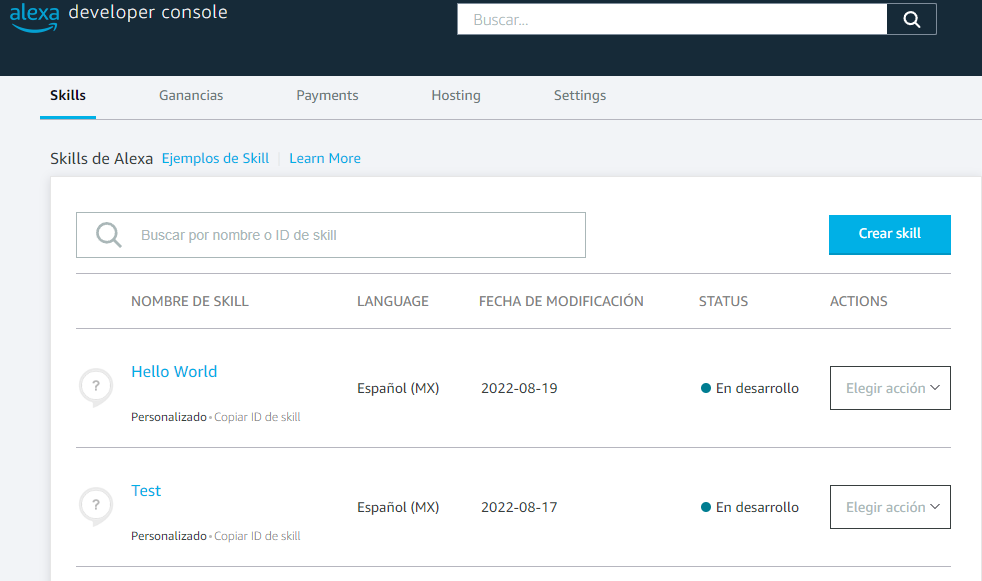
\includegraphics[width=0.60\textwidth]{Cap4/Figuras/Consola de Desarrollo de Alexa.png}
  \caption{División de la consola de desarrollo de Alexa.}
  \label{fig:43}
\end{figure}

La consola de desarrollo de Amazon también provee el flujo de creación de una skill por cada proyecto en desarrollo, en espera de certificación o publicado. El flujo definido se muestra a continuación:

\begin{enumerate}
  \item \textbf{Construcción (Build).} En esta sección se crean y configuran los siguientes elementos.
  \begin{itemize}
    \item Invocación o invocaciones.
    \item Intenciones.
    \item Declaraciones.
    \item Slots.
  \end{itemize}
  \item \textbf{Código (Code).} Apartado en el que se encuentra todo el código del comportamiento y funcionamiento de la skill. En este apartado se declara la función lambda, que es la función principal donde se programa el funcionamiento de la skill.
  \item \textbf{Pruebas (Test).} Contiene el simulador de Alexa, en el cual se pueden realizar pruebas sobre el funcionamiento de la skill.
  \item \textbf{Distribución (Distribution).} Información requerida para publicar la skill, tales como el nombre, descripción, logo, entre otros. En este apartado se define la siguiente información:
  \begin{itemize}
    \item Nombre público de la skill.
    \item Descripción breve de la skill.
    \item Descripción detallada de la skill.
    \item Funcionalidades generales de la skill.
    \item Frases de ejemplo para invocar la skill y manejar el flujo durante su ejecución.
    \item El ícono de la skill.
    \item La categoría de la skill.
    \item Palabras clave de la skill.
    \item URL de políticas de privacidad de la skill.
    \item URL de términos y usos de la skill.
    \item Determinar si la skill permite a los usuarios realizar pagos o gastar dinero real.
    \item Determinar si la skill permite acciones de compra a los usuarios.
    \item Determinar si la skill recopila información personal de los usuarios.
    \item Determinar si la skill está dirigida a usuarios menores a trece años.
    \item Determinar si la skill contiene publicidad.
    \item Aceptar los términos de cumplimiento de exportación de la skill.
    \item Instrucciones para realizar pruebas sobre la skill antes de ser publicada.
    \item Determinar si la skill es pública o su acceso está restringido a organizaciones de negocios.
    \item Decidir si se habilita la distribución automatizada de configuraciones regionales.
    \item Seleccionar la región en la que estará disponible la skill dentro de la tienda de skills.
  \end{itemize}
  \item \textbf{Certificación (Certification).} Sistema de validación de requerimientos y reglas para publicar la skill. En este apartado se presentan las siguientes acciones:
  \begin{itemize}
    \item Verificar que la skill no infringe políticas declaradas por Amazon.
    \item Información sobre las veces que se ha validado la skill y sus resultados.
    \item Historial de versiones de la skill.
    \item Un comparador para relacionar dos variantes de una misma skill y encontrar sus diferencias.
  \end{itemize}
  \item \textbf{Analítica (Analytics).} Información sobre la administración y analíticas del uso de la skill. Se puede encontrar la siguiente información:
  \begin{itemize}
    \item Un resumen del uso del modelo personalizado de la skill.
    \item La cantidad de veces que la skill se ha activado.
    \item Métricas del uso de sesiones, intenciones, declaraciones, entre otros.
    \item Información sobre el performance de la skill.
  \end{itemize}
\end{enumerate}

Estos apartados se encuentran organizados en pestañas dentro de la configuración de una skill, tal como se muestra en la Figura \ref{fig:44}.

\begin{figure}[H]
% \begin{figure}
  \centering
  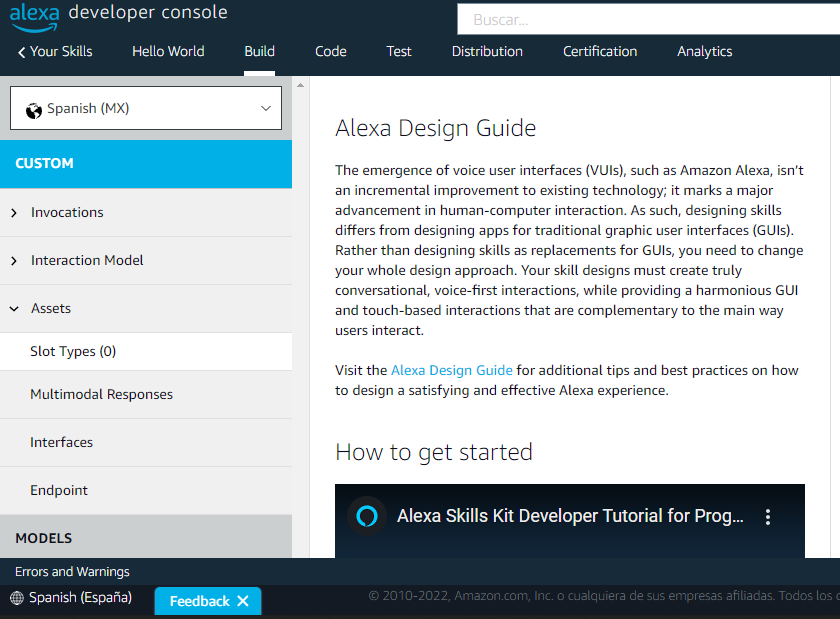
\includegraphics[width=0.60\textwidth]{Cap4/Figuras/Proceso de creacion de skill.png}
  \caption{Flujo del proceso de creación de skills.}
  \label{fig:44}
\end{figure}

%------------------------------------------------------------
%	Invocaciones
%------------------------------------------------------------

\subsubsection{Invocaciones}
\label{InvocacionescapIV}

% REFERENCIA
Amazon (2022g) una invocación como las diferentes formas en las que se puede activar una skill para comenzar a ejecutarse en el servicio de Alexa. La invocación de una skill puede ser ajustada y editada durante el proceso de desarrollo, sin embargo, la invocación no puede cambiar una vez que la skill ha sido certificada y publicada, por lo que es importante definir una invocación adecuada desde la etapa de diseño y configuración.

Las invocaciones se encuentran dentro de la sección llamada Build, tal como se muestra en la Figura \ref{fig:45}.

\begin{figure}[H]
% \begin{figure}
  \centering
  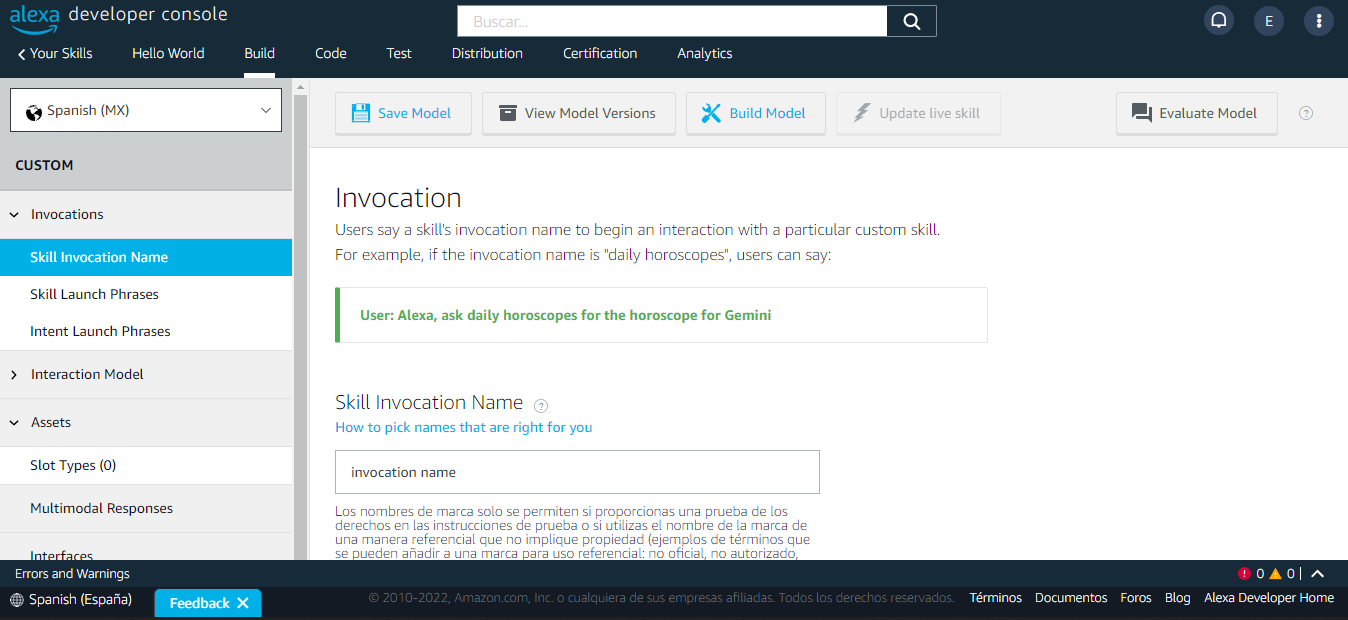
\includegraphics[width=0.70\textwidth]{Cap4/Figuras/Invocaciones.png}
  \caption{Definición de invocación o invocaciones de una skill.}
  \label{fig:45}
\end{figure}

Las invocaciones son un concepto que es aplicable únicamente para las skills personalizadas, ya que las skills pre-construidas requieren definirlas, debido a que los comandos se solicitan directamente.

% REFERENCIA
Amazon (2022g) señala que existen tres formas en las que los usuarios pueden activar una skill a partir de las invocaciones. Supongamos que tenemos una skill llamada Comida Mexicana, que tiene como objetivo proporcionar al usuario una gran variedad de platillos típicos mexicanos. A continuación se presentan las tres formas en las que se puede activar una skill por medio de las invocaciones:

\begin{itemize}
  \item \textbf{Invocaciones con solicitudes específicas.} Son invocaciones que en una misma frase incorpora la invocación con la solicitud de la tarea a realizar. Por ejemplo, $"$Alexa, dile a Comida Mexicana que me dé una receta de pozole$"$.
  \item \textbf{Invocaciones sin solicitudes.} Son invocaciones en las que se activa la skill sin necesidad de incorporar una solicitud. Por ejemplo $"$Alexa, abre Comida Mexicana$"$.
  \item \textbf{Invocación solicitada sólo por nombre.} Es la activación de una skill por medio de la invocación sin más información. Por ejemplo $"$Alexa, Comida Mexicana$"$.
\end{itemize}

Por otra parte, el equipo de Alexa recomienda cumplir con ciertos requisitos para que una invocación sea válida. Estos requisitos se presentan a continuación:

\begin{enumerate}
  \item El nombre de invocación de la skill no debe infringir los derechos de propiedad intelectual de una persona.
  \item El nombre de invocación debe ser un nombre compuesto de dos o más palabras, formando un identificador o frase, recomendablemente en el idioma en el que está desarrollada la skill para garantizar un claro reconocimiento por Alexa. El nombre de invocación de la skill puede tener una sola palabra únicamente si el nombre es exclusivo de la marca o propiedad intelectual del desarrollador o equipo de desarrollo.
  \item El nombre de invocación de la skill no puede incluir nombres de personas o lugares, a menos que se compongan de otra palabra.
  \item El nombre de invocación de la skill no puede ser de dos palabras si al menos una de ellas es un artículo o preposición.
  \item La invocación no puede contener ninguna palabra o frase de lanzamiento definida para activar alguna skill de Alexa. Por ejemplo las palabras $"$reproducir$"$, $"$comenzar$"$, $"$abre$"$, $"$empieza$"$, $"$lanza$"$, $"$pregunta$"$, entre otros.
  \item No se permiten palabras restringidas como $"$Alexa$"$, $"$Amazon$"$, $"$Echo$"$, $"$skill$"$, $"$aplicación$"$ o $"$app$"$.
  \item El nombre de invocación debe ser fácil de pronunciar y debe ser escrito correctamente, respetando acentos para las palabras que lo requieran, de lo contrario, no será lo mismo tener palabras como $"$árbol$"$ y $"$arbol$"$.
  \item Los puntos están permitidos para nombres que contienen abreviaturas o acrónimos, pero es importante establecer que estos se pronuncian como una serie de letras individuales.
  \item El nombre de la invocación no permite deletrear fonemas. Es decir, si se tiene un fonema como MCU, se escribiría como $"$m.c.u$"$ en lugar de $"$em si iu$"$.
  \item Se recomienda que el nombre de invocación no cree confusión con funcionalidades ya integradas en Alexa, con el fin de no ejecutar una funcionalidad diferente en lugar de la skill o viceversa.
  \item El nombre de la skill debe estar escrito en el idioma en que está desarrollada, ya que las palabras en otro idioma se superponen con palabras locales del idioma y puede reconocerse como una palabra diferente.
  \item Se recomienda que el nombre de invocación de la skill no sea demasiado genérico. Este debe ser distintivo para que la skill sea fácil de activar cuando se solicite.
\end{enumerate}

%------------------------------------------------------------
%	Intenciones
%------------------------------------------------------------

\subsubsection{Intenciones}
\label{IntencionescapIV}

% REFERENCIA
Las intenciones o intents son definidas por Amazon (2022k) como las funcionalidades que puede realizar una skill durante su ejecución. Estas se representan en forma de acciones para realizar una tarea específica.

La configuración y declaración de intenciones se encuentra dentro de la sección de construcción, tal como se muestra en la Figura \ref{fig:46}.

\begin{figure}[H]
% \begin{figure}
  \centering
  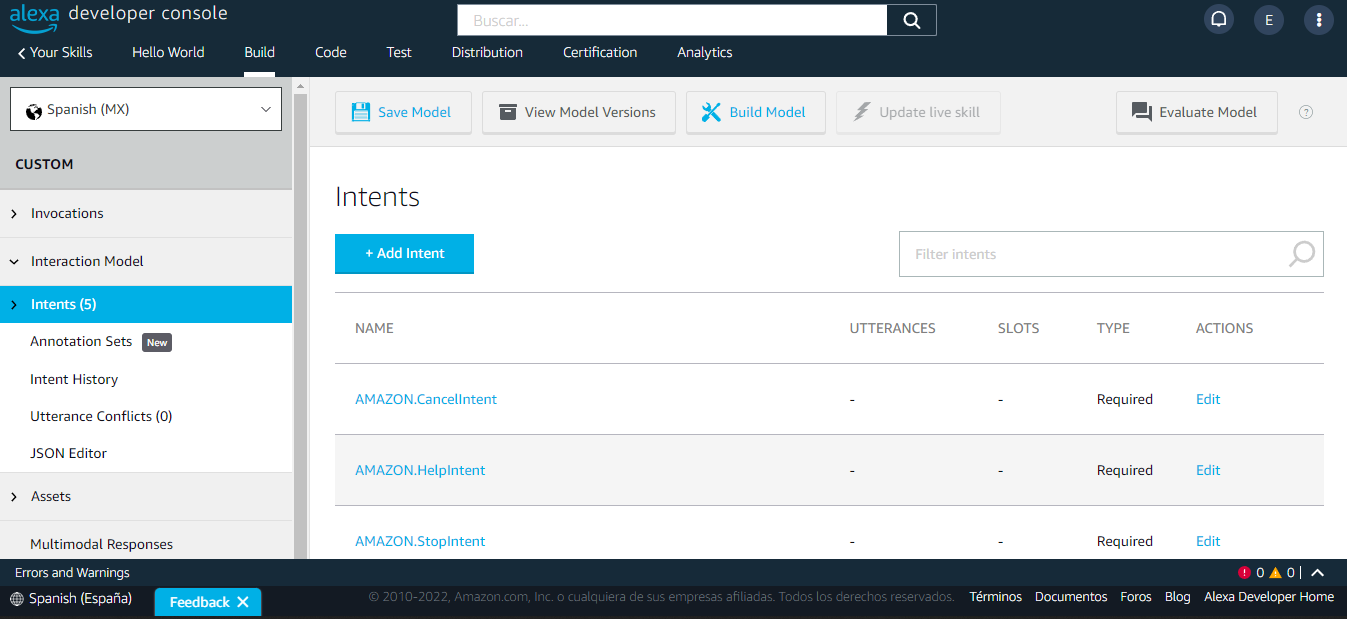
\includegraphics[width=0.70\textwidth]{Cap4/Figuras/Intenciones.png}
  \caption{Definición de intenciones de una skill.}
  \label{fig:46}
\end{figure}

Existen dos tipos de intenciones: predefinidas y personalizadas. Las intenciones predefinidas son acciones que ya se encuentran definidas y configuradas por la consola de desarrollo de Amazon.

% REFERENCIA
Entre las intenciones predefinidas, Amazon (2022k) define las siguientes:

\begin{itemize}
  \item \textbf{AMAZON.CancelIntent.} Es una intención definida para cancelar una acción en curso durante la skill.
  \item \textbf{AMAZON.HelpIntent.} Es una intención que puede ser configurada desde el código para ofrecer ayuda general sobre cómo usar la skill, con el fin de servir como guía al usuario.
  \item \textbf{AMAZON.StopIntent.} Es una intención que permite detener todas las acciones de una skill, terminando con el flujo y cerrando la skill.
  \item \textbf{AMAZON.NavigateHomeIntent.} Es una intención que se activa únicamente para dispositivos con pantalla, en la que se permite terminar la ejecución de una skill, devolviéndolos a la pantalla de inicio del dispositivo.
\end{itemize}

Existen otras intenciones predefinidas, que pueden ser agregadas manualmente desde la configuración de la consola de Amazon. Entre estas opciones se encuentran las siguientes intenciones:

\begin{itemize}
  \item \textbf{AMAZON.FallbackIntent.} Es una intención que permite dar alternativas para las expresiones que no hayan sido reconocidas por Alexa. Como respuesta de esta intención se puede dar detalle sobre la skill y cómo se puede interactuar con ella.
  \item \textbf{AMAZON.LoopOffIntent.} Permite al usuario la desactivación de un bucle para aquellas skills que desarrollan una funcionalidad de repetición. Por lo general. Por lo general esta intención se utiliza para skills que reproducen alguna lista de música o pistas.
  \item \textbf{AMAZON.LoopOnIntent.} Esta intención realiza la acción contraria a la intención anterior. Permite activar un bucle, generalmente para una lista de reproducción en skills que transmiten audio.
  \item \textbf{AMAZON.MoreIntent.} Es una intención que avanza el contenido actual para mostrar más contenido en dispositivos que tienen pantalla. Esta intención es similar al comportamiento de AMAZON.ScrollDownIntent y AMAZON.ScrollRightIntent.
  \item \textbf{AMAZON.NavigateSettingsIntent.} Esta intención funciona para dispositivos que cuentan con pantalla. Permite llevar al usuario a la pantalla de configuración del dispositivo y al salir regresará a la skill.
  \item \textbf{AMAZON.NextIntent.} Esta intención permite navegar a un siguiente elemento de una lista. En caso de tratarse de una skill que transmite audio, esta intención permite saltar a la siguiente reproducción.
  \item \textbf{AMAZON.NoIntent.} Facilita al usuario dar una respuesta negativa a preguntas del tipo $"$sí$"$ o $"$no$"$.
  \item \textbf{AMAZON.PageDownIntent.} Baja la vista a la siguiente pantalla de una interfaz en dispositivos que cuentan con pantalla.
  \item \textbf{AMAZON.PageUpIntent.} Sube la vista a una pantalla anterior de una interfaz en dispositivos que cuentan con pantalla.
  \item \textbf{AMAZON.PauseIntent.} Esta intención permite pausar el flujo de una skill, tal como pausar un videojuego o un audio en una lista de reproducción.
  \item \textbf{AMAZON.PreviousIntent.} Esta skill permite navegar a un elemento previo de una lista. En caso de tratarse de una skill que transmite audio, esta intención permite retroceder a la reproducción anterior.
  \item \textbf{AMAZON.RepeatIntent.} Permite repetir la última acción realizada por una skill.
  \item \textbf{AMAZON.ResumeIntent.} Reanuda o continua con alguna acción previamente puesta en pausa de una skill.
  \item \textbf{AMAZON.ScrollDownIntent.} Permite desplazar la interfaz hacia abajo de los dispositivos que cuentan con pantalla.
  \item \textbf{AMAZON.ScrollLeftIntent.} Permite desplazar la interfaz a la izquierda de los dispositivos que cuentan con pantalla.
  \item \textbf{AMAZON.ScrollRightIntent.} Permite desplazar la interfaz a la derecha de los dispositivos que cuentan con pantalla.
  \item \textbf{AMAZON.ScrollUpIntent.} Permite desplazar la interfaz hacia arriba de los dispositivos que cuentan con pantalla.
  \item \textbf{AMAZON.SelectIntent.} Permite al usuario indicar la selección de un elemento, por lo general de un listado de registros.
  \item \textbf{AMAZON.SendToPhoneIntent.} Se permite enviar información o resultados de una skill al teléfono a través de la app de Alexa en dispositivos móviles.
  \item \textbf{AMAZON.ShuffleOffIntent.} Permite desactivar el modo aleatorio en la skill. Por lo general, esta intención es usada para skills que transmiten audio en una lista de reproducción.
  \item \textbf{AMAZON.ShuffleOnIntent.} Permite activar el modo aleatorio de la skill. Generalmente para skills que transmiten audio en una lista de reproducción.
  \item \textbf{AMAZON.StartOverIntent.} Permite reiniciar una acción a un punto específico. Tal como reiniciar un juego o una pista de audio.
  \item \textbf{AMAZON.YesIntent.} Permite proporcionar una respuesta positiva para respuesta de preguntas del tipo $"$si$"$ o $"$no$"$.
\end{itemize}

Por otro lado, las intenciones personalizadas son intenciones que se crean manualmente desde la consola de desarrollo de Amazon, en la que se realizan las configuraciones necesarias para llevar a cabo acciones específicas fuera de las intenciones ya definidas por Amazon. Es recomendable que cuando se crea una nueva intención personalizada, esta debe nombrarse terminando con la palabra \textit{intent}. Por ejemplo, en la skill de ejemplo \textit{Comida Mexicana} podemos tener una intención que permita leer las instrucciones para preparar un platillo que pude ser llamada \textit{InstructionsIntent} o \textit{StartCookingIntent}.

%------------------------------------------------------------
%	Declaraciones
%------------------------------------------------------------

\subsubsection{Declaraciones}
\label{DeclaracionescapIV}

% REFERENCIA
Amazon (2022h), señala que las declaraciones o utterances son las diferentes frases que activan una intención. Cada intención tiene un apartado para definir las declaraciones como se muestra en la Figura \ref{fig:47}.

\begin{figure}[H]
% \begin{figure}
  \centering
  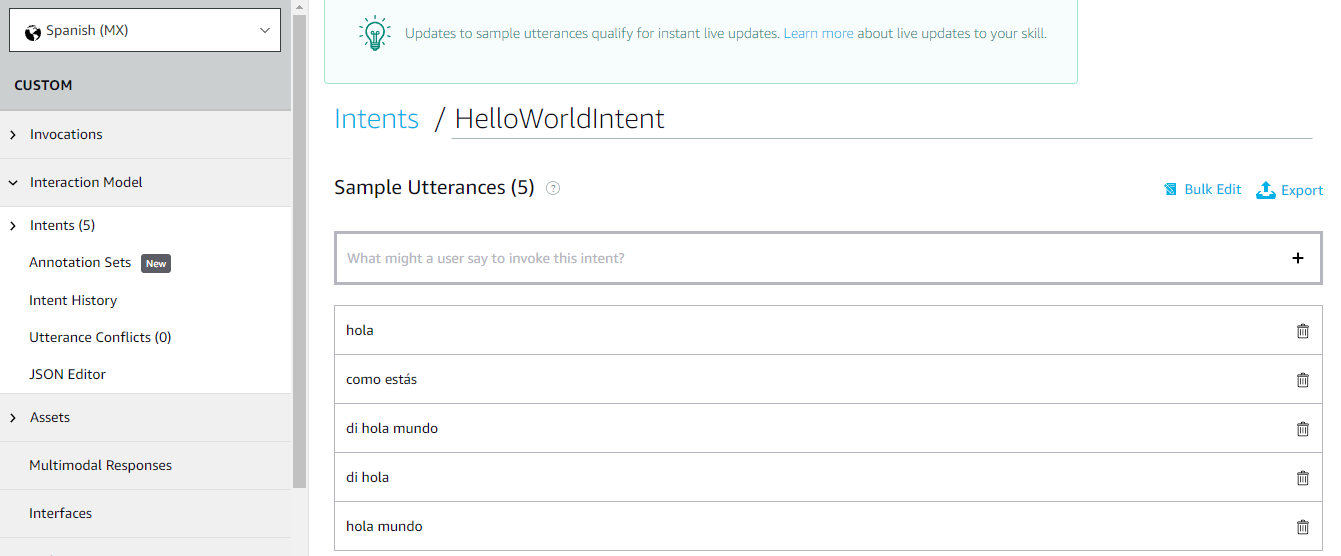
\includegraphics[width=0.70\textwidth]{Cap4/Figuras/Declaraciones.png}
  \caption{Definición de declaraciones de una intención de una skill.}
  \label{fig:47}
\end{figure}

Las intenciones predefinidas ya cuentan con declaraciones asociadas a su comportamiento, sin embargo, es posible definir declaraciones personalizadas extra en una invocación predefinida.

Por otro lado, cuando se crea una intención personalizada, es necesario definir al menos una declaración para poder activarla. Se recomienda fuertemente que las declaraciones estén diseñadas en el idioma en la que está definida la skill. Supongamos que tenemos la intención \textit{InstructionsIntent} que permite conocer las instrucciones para cocinar un platillo mexicano. Algunas de las declaraciones para poder activar la intención podrían ser las siguientes:

\begin{itemize}
  \item Dime las instrucciones de un platillo.
  \item Lee las instrucciones de un platillo.
  \item Comienza con el platillo.
  \item Quiero saber más información del platillo.
\end{itemize}

Este tipo de declaraciones puede ser aplicado tanto para invocaciones predefinidas como para invocaciones personalizadas. Sin embargo, existen otro tipo de declaraciones, las cuales permiten recabar información en forma de parámetros o argumentos dentro del mismo comando. A estos argumentos se les conoce como slots. Algunas de las declaraciones con slots para poder activar la intención \textit{InstructionsIntent} podrían ser las siguientes.

\begin{itemize}
  \item Dime las instrucciones para cocinar tacos al pastor.
  \item Comienza a cocinar pozole.
  \item Quiero aprender a cocinar alambre de bistec.
\end{itemize}

En las declaraciones anteriores, se solicita información específica que pasa por medio de argumentos, tal como tacos al pastor, pozole o alambre de bistec. Como estos datos son parámetros en la declaración, la estructura con slots de las mismas declaraciones se vería como sigue:

\begin{itemize}
  \item Dime las instrucciones para cocinar \{nombrePlatillo\}.
  \item Comienza a cocinar \{nombrePlatillo\}.
  \item Quiero aprender a cocinar \{nombrePlatillo\}.
\end{itemize}

En donde la variable \textit{nombrePlatillo} corresponde a un valor específico.

% REFERENCIA
Amazon (2022h) señala que una declaración se forma de la estructura descrita en la Figura \ref{fig:48}.

\begin{figure}[H]
% \begin{figure}
  \centering
  
\includegraphics[width=0.70\textwidth]{Cap4/Figuras/Estructura de Declaraciones.jpg}
  \caption{Estructura de una declaración o utterance. Amazon (2022h).}
  \label{fig:48}
\end{figure}

Donde:

\begin{itemize}
  \item \textbf{SearchAction.} Es un objeto que realiza la búsqueda de una acción que el usuario quiere ejecutar.
  \item \textbf{object.} Es un objeto en el que se identifican las entidades involucradas en una declaración y con el que se puede operar.
  \item \textbf{attributes.} Son aquellos valores que pasan por medio de uno o más slots. La forma en la que se accede a estos valores es por medio de object.
\end{itemize}

%------------------------------------------------------------
%	Slots
%------------------------------------------------------------

\subsubsection{Slots}
\label{SlotscapIV}

% REFERENCIA
Como se comentó anteriormente, Amazon (2022i) define los slots como argumentos que son proporcionados en una declaración. Estos argumentos son una herramienta útil para recabar información de diferentes tipos.

La configuración y definición de los slots usados en las declaraciones de una intención se encuentra en la sección de construcción de una skill, tal como se muestra en la Figura \ref{fig:49}.

\begin{figure}[H]
% \begin{figure}
  \centering
  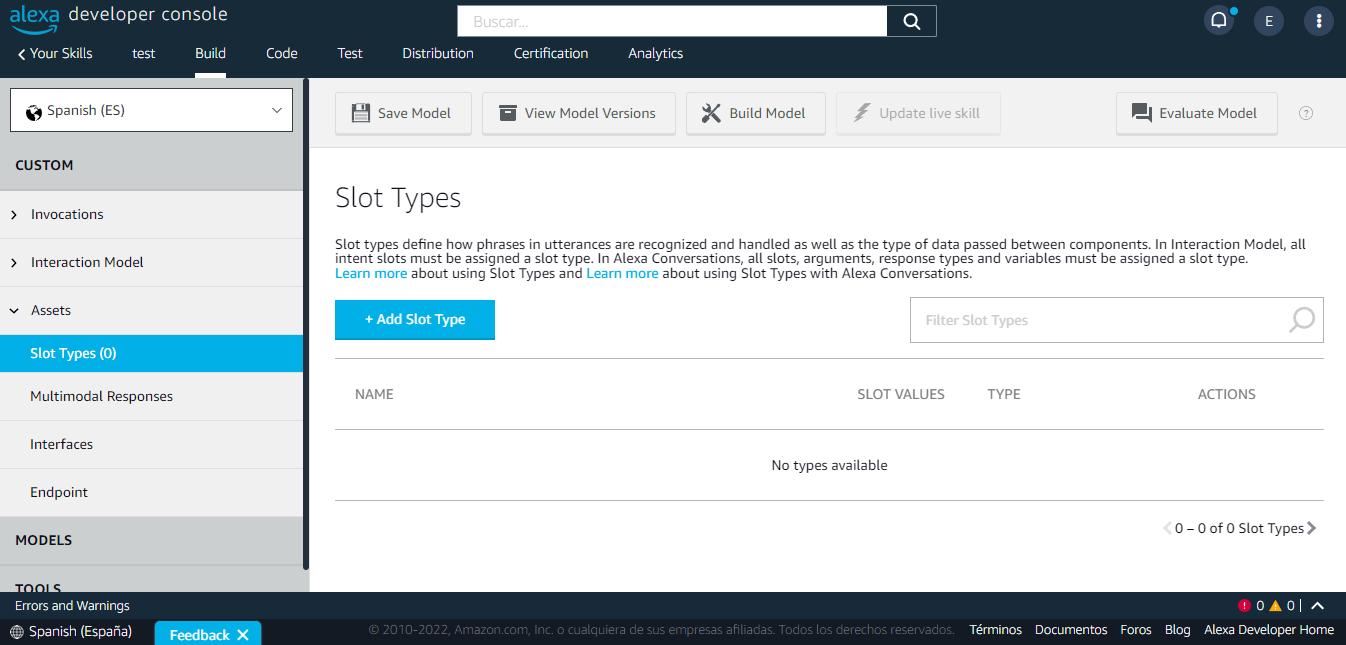
\includegraphics[width=0.70\textwidth]{Cap4/Figuras/SlotTypes.png}
  \caption{Definición de slots para las declaraciones de una skill.}
  \label{fig:49}
\end{figure}

Existen dos tipos de slots: slots predefinidos y slots personalizados. A su vez, los slots predefinidos se dividen en dos categorías. Por una parte, existen slots que reconocen valores en una lista de sugerencias que puede ser extendida por el desarrollador. Por otra parte, se tienen slots que convierten un dato en información específica que no está definida en una lista, por lo que estos no pueden ser extendidos por el desarrollador.

% REFERENCIA
Amazon (2022i) señala que entre los slots predefinidos se encuentran los siguientes:

\begin{itemize}
  \item \textbf{AMAZON.Actor.} Es un slot que almacena una lista con nombres de actores y actrices.
  \item \textbf{AMAZON.Airline.} Contiene una lista con gran variedad de nombres de aerolíneas.
  \item \textbf{AMAZON.Airport.} Almacena una gran variedad de nombres de aeropuertos.
  \item \textbf{AMAZON.Anaphor.} Contiene palabras que representan una anáfora. Tales como $"$este$"$, $"$eso$"$, $"$esa$"$, etc.
  \item \textbf{AMAZON.Animal.} Lista con una gran variedad de nombres de animales.
  \item \textbf{AMAZON.Artist.} Lista con una gran variedad de nombres completos de artistas.
  \item \textbf{AMAZON.Book.} Listado de algunos títulos de libros.
  \item \textbf{AMAZON.City.} Provee un listado de ciudades comúnmente usadas localmente, según la configuración de idioma en que está desarrollada la skill.
  \item \textbf{AMAZON.Color.} Listado con los nombres de los colores.
  \item \textbf{AMAZON.Corporation.} Listado con el nombre completo de varias corporaciones.
  \item \textbf{AMAZON.Country.} Listado del nombre de los países o regiones del mundo.
  \item \textbf{AMAZON.CreativeWorkType.} Listado de palabras usadas en trabajos creativos, tal como $"$canción$"$, $"$show$"$, $"$escenario$"$, etc.
  \item \textbf{AMAZON.DayOfWeek.} Listado de los días de la semana basados en el calendario.
  \item \textbf{AMAZON.FictionalCharacter.} Listado de nombres de personajes ficticios de libros, películas, televisión, entre otros.
  \item \textbf{AMAZON.FirstName.} Listado de gran cantidad de nombres usados localmente, por ejemplo, los nombres más usados por hablantes mexicanos para una skill configurada con localidad en México.
  \item \textbf{AMAZON.Food.} Listado de nombres de diferentes platillos.
  \item \textbf{AMAZON.Genre.} Listado de diferente tipo de géneros que describen música, libros, espectáculos de televisión, entre otros.
  \item \textbf{AMAZON.Language.} Listado con diferentes idiomas, tal como español, inglés, chino, etc.
  \item \textbf{AMAZON.Month.} Listado del nombre de los meses en el calendario.
  \item \textbf{AMAZON.Movie.} Listado de gran variedad de películas.
  \item \textbf{AMAZON.MusicAlbum.} Listado de nombres de álbumes musicales.
  \item \textbf{AMAZON.MusicGroup.} Listado del nombre de diferentes grupos musicales, tales como bandas, orquestas, coros e incluso artistas independientes.
  \item \textbf{AMAZON.Musician.} Listado del nombre completo de algunos músicos.
  \item \textbf{AMAZON.MusicRecording.} Listado del nombre de varias canciones grabadas.
  \item \textbf{AMAZON.Person.} Listado de nombres completos de personas reales o ficticias.
  \item \textbf{AMAZON.RadioChannel.} Listado del nombre de diferentes canales o estaciones de radio.
  \item \textbf{AMAZON.Region.} Provee una lista de países y regiones generalmente usados por los hablantes de la localidad de la skill.
  \item \textbf{AMAZON.RelativePosition.} Provee un listado de palabras que reconocen la posición relativa de un elemento en una lista, tal como $"$primero$"$ o $"$último$"$.
  \item \textbf{AMAZON.Room.} Listado del nombre de diferentes habitaciones o cuartos de una casa y otras edificaciones.
  \item \textbf{AMAZON.Sport.} Listado con el nombre de diferentes deportes.
  \item \textbf{AMAZON.StreetName.} Listado con el nombre de diferentes calles y avenidas.
  \item \textbf{AMAZON.TVSeries.} Listado con una gran cantidad de títulos y nombres de series de televisión.
  \item \textbf{AMAZON.VideoGame.} Listado con el nombre de varios videojuegos.
  \item \textbf{AMAZON.VisualModeTrigger.} Listado de palabras relacionadas a la espera de una respuesta visual, tal como $"$muestra$"$ o $"$despliega$"$.
\end{itemize}

Cabe mencionar que los valores proporcionados en los slots anteriores podrían no considerar datos específicos que requiere una skill. Es por ello que la consola de Amazon provee la posibilidad de extender los valores de estas listas, definiendo aquellos valores que también puede considerar.

Sin embargo, se cuentan con los slots predefinidos que no se basan en un listado de palabras o definiciones, sino que transforman una entrada a un tipo de valor específico, tal como los números. Entre estos slots se encuentran los siguientes:

\begin{itemize}
  \item \textbf{AMAZON.DATE.} Convierte palabras que indican una fecha, tales como “hoy”, “mañana”, “agosto” y los convierte a un formato de fecha, tal como “2015-07-00T9”.
  \item \textbf{AMAZON.DURATION.} Convierte palabras que indican una duración, tal como “una hora”, “dos semanas”, y los convierte a una duración numérica del tipo “PT5M”.
  \item \textbf{AMAZON.FOUR\_DIGIT\_NUMBER.} Convierte palabras a un número de cuatro dígitos, por ejemplo la frase “cinco, cuatro, tres, dos” se convierte a un valor numérico como “5432”.
  \item \textbf{AMAZON.NUMBER.} Convierte palabras que representan un dígito en un número, tal como “seis” a “6”.
  \item \textbf{AMAZON.Ordinal.} Convierte palabras que representan números ordinales en dígitos, tal como “tercero” a “3”.
  \item \textbf{AMAZON.PhoneNumber.} Convierte palabras que representan un número telefónico a un dígito con representación a números de teléfono locales, nacionales e internacionales.
  \item \textbf{AMAZON.SearchQuery.} Convierte una palabra o frase en una oración que podría ser ingresada en un motor de búsqueda estándar.
  \item \textbf{AMAZON.TIME.} Convierte palabras que indican tiempo, tal como “seis de la mañana” y los convierte a un valor con formato horario como “06:00” con un tiempo de 24 horas.
\end{itemize}

Sin embargo,  a pesar de la gran variedad de slots predefinidos en la consola de Amazon, cabe la posibilidad de que se necesite un slot con valores específicos para alguna skill. A estos slots se les conoce como slots personalizados, en los que se determinan los valores que puede reconocer.

% REFERENCIA
Amazon (2022i) señala que los valores definidos para un slot personalizado puede ser cualquier palabra que pueda ser pronunciada por un usuario. De lo contrario, es muy probable que no se pueda reconocer alguna palabra que no se encuentre definida en un diccionario del idioma en que está configurada la skill.

Es importante considerar que las frases que contienen acrónimos, se deben definir en los valores del slot en letras mayúsculas o en letras minúsculas seguidos de un punto. Por ejemplo, si se requiere tener como valor el acrónimo CDMX, este debe estar definido como $"$CDMX$"$ o $"$c. d. m. x.$"$ como valor del slot.

Al momento de crear un slot, cabe la posibilidad de agregarle sinónimos y un identificador, tal como se muestra en la Figura \ref{fig:410}. Los sinónimos pueden ser usados como alternativas al valor original de un elemento de la lista de valores.

\begin{figure}[H]
% \begin{figure}
  \centering
  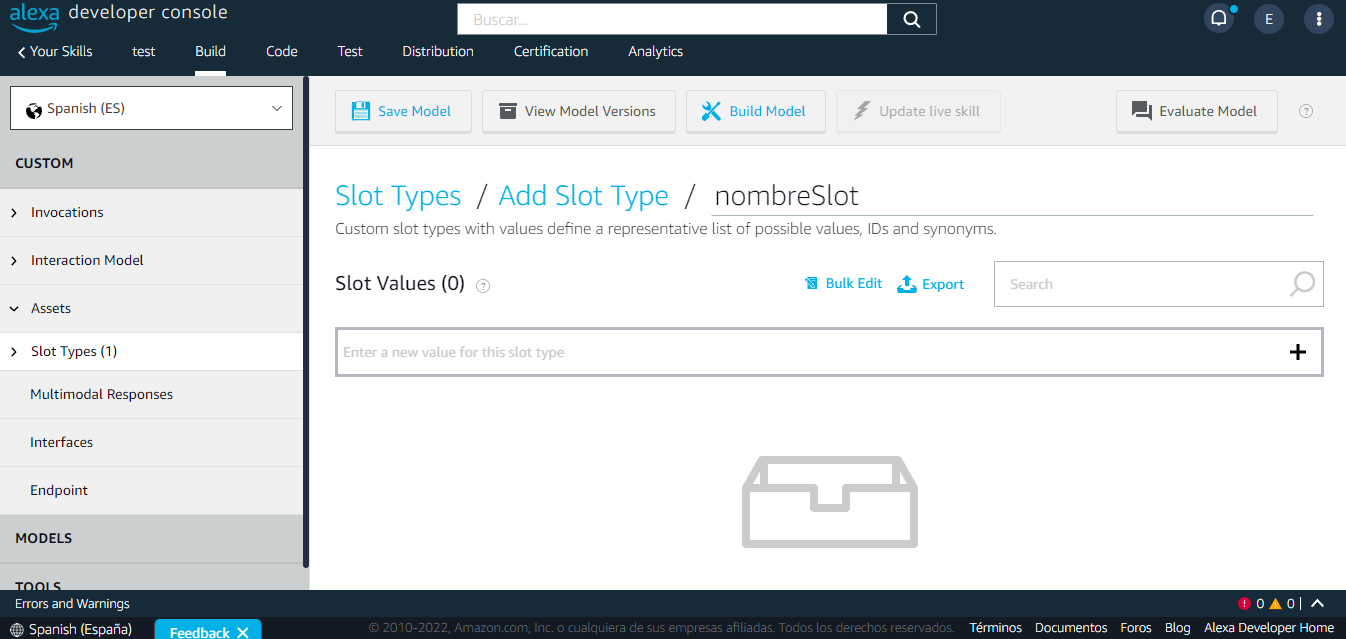
\includegraphics[width=0.70\textwidth]{Cap4/Figuras/SlotTypesCreation.png}
  \caption{Ejemplo de sinónimos de un slot.}
  \label{fig:410}
\end{figure}

%------------------------------------------------------------
%	Función Lambda
%------------------------------------------------------------

\subsubsection{Función Lambda}
\label{FuncionLambdacapIV}

% REFERENCIA
El código donde se implementan las invocaciones de la skill se definen en una función llamada función Lambda. Amazon (2022j) señala que existen dos formas de crear una función Lambda: la primera forma consiste en hospedar el código en los servicios de la consola de desarrollo de Alexa, en la que se permite desarrollar en los lenguajes de programación Python y Node.js; la segunda forma consiste en hospedar la función Lambda en el servicio de Amazon Web Services (AWS), llamado AWS Lambda, en la que se da la posibilidad de programar en los lenguajes de programación Node.js, Java, Python, Go, Ruby y C\#.

La función lambda que se hospeda en la consola de desarrollo de Amazon, se encuentra definida en la sección llamada Code del flujo de implementación de una skill. Para el lenguaje de programación Node.js, se encuentra definida en el archivo index.js, dentro del directorio llamado lambda. Mientras que para el lenguaje de programación Python, se encuentra en el archivo llamado \textit{lambda\_function.py}, dentro del directorio llamado lambda.

Esta función se encuentra predefinida en la sección de código, tal como se muestra en la Figura \ref{fig:411}.

\begin{figure}[H]
% \begin{figure}
  \centering
  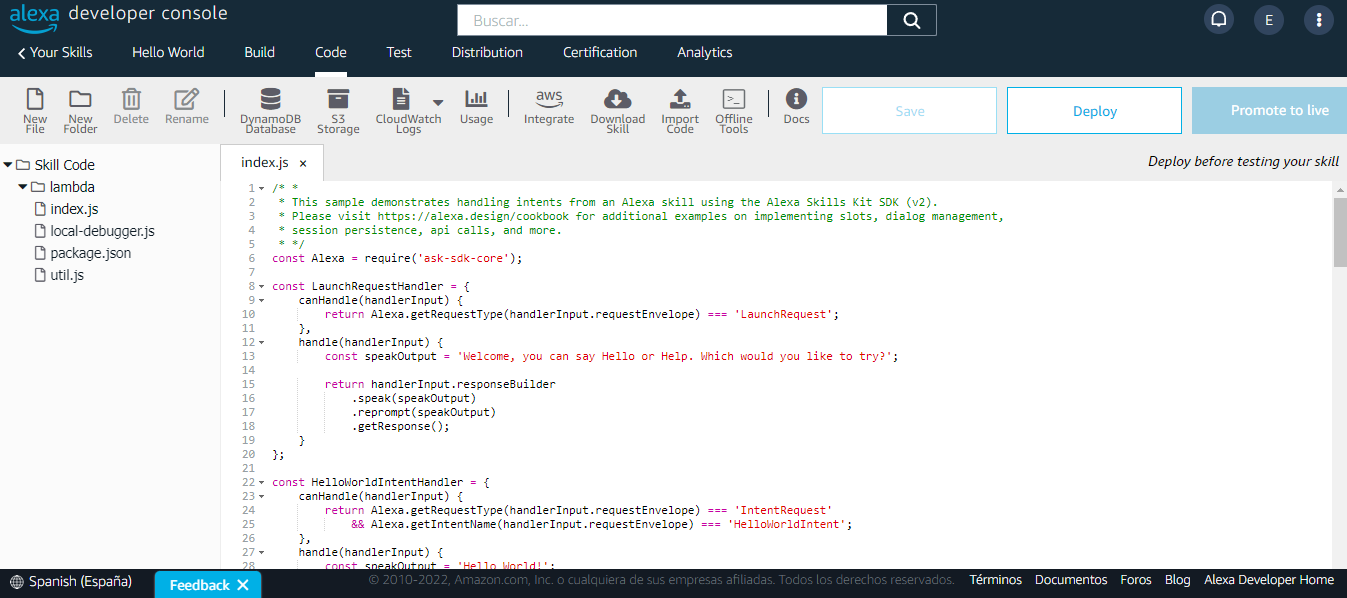
\includegraphics[width=0.70\textwidth]{Cap4/Figuras/Funcionlambda.png}
  \caption{Declaración de la función Lambda de una skill.}
  \label{fig:411}
\end{figure}

La función importa por omisión la biblioteca llamada \textit{ask\_sdk\_core}, la cual contiene funcionalidades para poder programar las acciones básicas en Alexa, tales como las siguientes:

\begin{itemize}
  \item El constructor de skills.
  \item El controlador de solicitudes definidas para el reconocimiento de las intenciones por reconocimiento por voz.
  \item El lanzador de inicio de ejecución de la skill, con el reconocimiento del nombre de invocación de la skill.
  \item El reconocedor de nombres de las intenciones definidas de la skill.
  \item El constructor de respuestas de las intenciones de la skill.
\end{itemize}

Cabe mencionar que existen más propiedades que pueden ser importadas manualmente para implementar funcionalidades extra.

La función contiene un conjunto de controladores de solicitudes, los cuales se denominan \textit{Handlers}. Estos permiten definir el comportamiento específico de una intención, con el que se provee una respuesta a la acción por medio del constructor de respuestas.

Existen dos tipos de Handlers: los handlers que están a la espera de solicitudes de tipo LaunchRequest y los que están a espera de solicitudes IntentRequest.

\begin{itemize}
  \item \textbf{LaunchRequest.} Existe sólo un handler con este tipo de solicitud en la Lambda. Este handler se ejecuta cuando un usuario dice un comando de activación de la skill. Da como respuesta la bienvenida o introducción general a la skill, así como sugerencias a un comando de inicio para seguir el flujo. De manera predefinida, al crear una nueva skill con Python, la consola de desarrollo de Alexa genera el siguiente ejemplo de un handler con solicitud de tipo LaunchRequest.
  \begin{tcolorbox}[colback=white!25!white,colframe=blue]
    \begin{minted}{python}
class LaunchRequestHandler(AbstractRequestHandler):
  """Handler for Skill Launch."""
  def can_handle(self, handler_input):
    # type: (HandlerInput) -> bool
  
    return ask_utils.is_request_type("LaunchRequest")(handler_input)
  
  def handle(self, handler_input):
    # type: (HandlerInput) -> Response
    speak_output = "Welcome, you can say Hello or Help."+
      "Which would you like to try?"
  
    return (
      handler_input.response_builder
        .speak(speak_output)
        .ask(speak_output)
        .response
    )
    \end{minted}
  \end{tcolorbox}
  \item \textbf{IntentRequest.} Son aquellos handlers que se ejecutan cuando una intención es activada. Este tipo de handlers reciben un parámetro adicional, que corresponde al nombre exacto de la intención que se quiere ejecutar. De manera predefinida, al crear una nueva skill con Python, la consola de desarrollo de Alexa genera el siguiente ejemplo de un IntentRequest.
  \begin{tcolorbox}[colback=white!25!white,colframe=blue]
    \begin{minted}{python}
class HelloWorldIntentHandler(AbstractRequestHandler):
  """Handler for Hello World Intent."""
  def can_handle(self, handler_input):
    # type: (HandlerInput) -> bool
    return ask_utils.is_intent_name("HelloWorldIntent")(handler_input)

  def handle(self, handler_input):
    # type: (HandlerInput) -> Response
    speak_output = "Hello World!"

    return (
      handler_input.response_builder
        .speak(speak_output)
        # .ask("add a reprompt if you want to keep the session
        # open for the user to respond")
        .response
    )
    \end{minted}
  \end{tcolorbox}
\end{itemize}

Los slots que intervienen en un handler también se transmiten como parámetros para poder ser accesibles dentro de la definición de la función que lo implementa. A estos se accede de forma diferente, dependiendo del lenguaje de programación. Para el caso de Python se usa la siguiente sintaxis.

\begin{tcolorbox}[colback=white!25!white,colframe=blue]
  \begin{minted}{python}
handler_input.request_envelope.request.intent.slots['slotName']
  \end{minted}
\end{tcolorbox}

Donde \textit{slotName} corresponde al nombre del slot que se quiere recuperar. Este ya cuenta con todas las propiedades definidas en el proceso de definición del slot.

Es importante mencionar que estos handlers pueden definirse en el archivo pero no son reconocidos automáticamente por el constructor de la skill. Estos deben ser agregados como parámetros a la función de definición de handlers para cambiar a un estado de activación para el reconocimiento por voz de los comandos asociados. La sintaxis para activar los handlers en Python de una skill se presenta a continuación.

\begin{tcolorbox}[colback=white!25!white,colframe=blue]
  \begin{minted}{python}
sb = SkillBuilder()
sb.add_request_handler(LaunchRequestHandler())
sb.add_request_handler(Intent1Handler())
sb.add_request_handler(Intent2Handler())
…
sb.add_request_handler(IntentNHandler())
  \end{minted}
\end{tcolorbox}

%------------------------------------------------------------
%	Simulador de Alexa
%------------------------------------------------------------

\subsubsection{Simulador de Alexa}
\label{SimuladorcapIV}

% REFERENCIA
Amazon (2022l) señala que existe una página en la que se pueden realizar pruebas del funcionamiento de la skill, para corroborar su correcto comportamiento con el reconocimiento de voz, intenciones, declaraciones, slots, respuestas progresivas y la resolución de entidades. Amazon (2022l) recomienda que antes de realizar pruebas a la skill, se configuren las características mínimas requeridas para su funcionamiento en la consola de desarrollo, tales como la definición de intenciones, la configuración de declaraciones y la implementación del código.

El apartado llamado \textit{Test}, provee tres formas diferentes para poder realizar pruebas en una skill. Cada una de estas formas está enfocada a características específicas como las siguientes:

\begin{itemize}
  \item \textbf{Simulador de Alexa.} Provee la posibilidad de realizar pruebas en una skill por medio de texto y voz, además, provee las herramientas necesarias para manejar la skill como si se estuviera utilizando un dispositivo con el servicio de Alexa integrado.
  \item \textbf{Manual de JSON.} Permite ingresar objetos con el formato JSON directamente a las solicitudes de la skill, así como ver la respuesta JSON que la skill lanza como respuesta. Este manual es muy útil para mandar información a lambdas de AWS por medio de endpoints, que son URLs de puntos de entrada para un servicio de AWS, hospedados en regiones específicas.
  \item \textbf{Voz y tonos.} Alexa permite dar respuestas con tonos diferentes a la tonalidad habitual, por medio de un mecanismo llamado Speech Synthesis Markup Language (SSML). El SSML permite que Alexa exprese frases con diferentes tonos, tales como emoción, tristeza, susurros, pausas largas, entre otros. El paso de datos por archivos con el formato SSML permite interactuar con la forma en que Alexa podría dar diferentes respuestas.
\end{itemize}

% REFERENCIA
Amazon (2022m) menciona que el simulador de Alexa también permite tener una vista previa a los servicios de Alexa Presentation Language (APL), que permite tener una interfaz gráfica para aquellos dispositivos que cuenten con una pantalla. En esa configuración se puede observar cómo se vería el resultado final en diferentes dispositivos con Alexa integrada que cuentan con pantalla, tales como dispositivos Hub Round Small, Hub Landscape Small, Hub Landscape Medium, Hub Landscape Large, .Hub Landscape Extra Large, Hub Portrait Medium, TV Landscape Extra Large, Mobile Small, Mobile Medium y Mobile Large.

% REFERENCIA
Amazon (2022m) señala que es necesario cumplir ciertos requisitos previos para habilitar los test en el simulador de Alexa.

\begin{itemize}
  \item Sólo sirve para skills personalizadas.
  \item Se debe configurar un endpoint válido para la skill. Por lo que es importante implementar un punto de finalización para el término de la ejecución de la skill.
  \item La skill se debe habilitar dentro de la página de Test.
  \item Para skills de video, es necesario habilitar la skill en la aplicación de Alexa, completando la información requerida.
\end{itemize}

Así mismo, es posible habilitar otras herramientas para realizar pruebas sobre la skill desde el simulador de Alexa. Entre estas se encuentran las siguientes opciones.

\begin{itemize}
  \item \textbf{I/O de la skill.} Permite visualizar las cargas útiles sobre las solicitudes y respuestas de Alexa en formato JSON. Se muestran las solicitudes hechas por el usuario y la respuesta de diálogo con toda su configuración en un objeto en formato JSON.
  \item \textbf{Visualizador de dispositivos con pantalla.} Se muestra un aproximado de cómo se vería la interfaz gráfica en pantalla por medio del servicio de APL.
  \item \textbf{Registros de dispositivos.} Permite visualizar los eventos enviados a Alexa, así como las directivas en cada interacción con la skill.
  \item \textbf{Alexa Smart Home (Beta).} permite visualizar los eventos de tipo ChangeReport que la skill envía como enlaces a eventos de Alexa. Esta funcionalidad sólo está disponible para skills enfocadas a hogares inteligentes.
\end{itemize}

% REFERENCIA
Finalmente, Amazon (2022m) señala que el simulador de Alexa provee un sistema de depuración de intenciones, habilitando la funcionalidad llamada Device Log, en la que se muestran todas las intenciones devueltas por la skill en formato JSON. Esta forma de depuración es útil para resolver expresiones y casos no previstos en las intenciones definidas.

El simulador de Alexa se encuentra en la sección de pruebas de la skill, tal como se muestra en la Figura \ref{fig:412}.

\begin{figure}[H]
% \begin{figure}
  \centering
  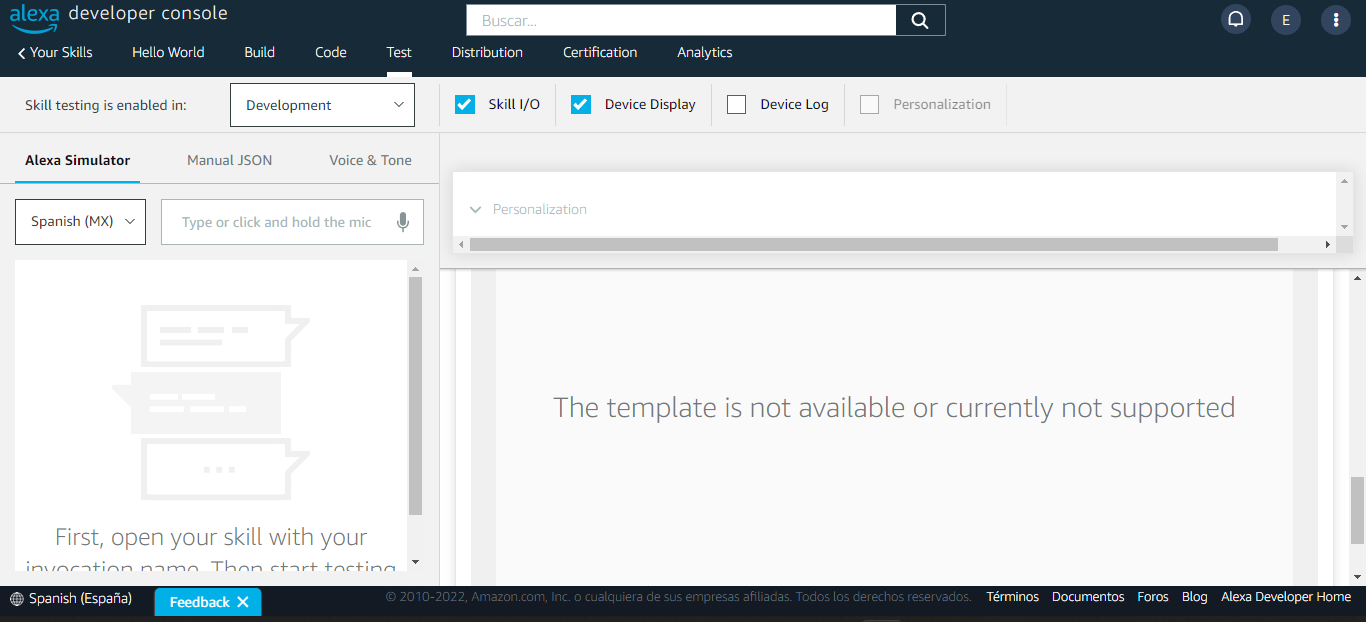
\includegraphics[width=0.70\textwidth]{Cap4/Figuras/Simulador.png}
  \caption{Simulador de Alexa para las pruebas de una skill.}
  \label{fig:412}
\end{figure}

%------------------------------------------------------------
%	Análisis del problema
%------------------------------------------------------------

\section{Análisis del problema}
\label{AnalisisProblemacapIV}

El análisis del problema es una etapa fundamental para identificar las oportunidades de mejora que pueden considerarse para atacar un problema de una forma efectiva, así como el desarrollo de una solución que satisfaga las necesidades del usuario, en este análisis, basados en el diseño centrado en el usuario.

A continuación se presenta una descripción que detalla la identificación de los principales problemas presentados durante la búsqueda e investigación de información, así como las oportunidades de mejora encontradas en cada paso del Modelo Gavilán.

%------------------------------------------------------------
%	Identificación del problema
%------------------------------------------------------------

\subsection{Identificación del problema}
\label{IdentificacionProblemacapIV}

En el Diplomado Internacional de Innovación en la Docencia Universitaria del año 2020, se consideraron diferentes aspectos y características sobre los mayores problemas con los que se enfrentan los alumnos al momento de realizar una investigación.

Como parte de las actividades del diplomado, los profesores expresaron diferentes puntos de vista sobre la deficiencia del proceso de búsqueda de información que generalmente cometen los alumnos. Muchos de los profesores comparten puntos similares que notaron durante el análisis de la actividad, entre los que destacan los siguientes:

\begin{itemize}
  \item Gran parte de la investigación se basa en un proceso de copiar y pegar información.
  \item Dado que la información, por lo general se copia y pega, no se analiza el contenido de la investigación.
  \item No se establece un objetivo para la investigación, por lo que se busca directamente el contenido, omitiendo puntos relevantes e insertando información que no forma parte de los límites de la investigación.
  \item La mayor fuente de información que se utiliza es la Internet. Donde se selecciona, por lo general, las primeras páginas que resultan de la búsqueda. Cabe resaltar que estas páginas no necesariamente son confiables por estar en las primeras posiciones de la búsqueda.
  \item Generalmente se selecciona la fuente de información que describa la mayor cantidad de información sobre el contenido solicitado en la investigación.
  \item El proceso que siguen los alumnos para determinar si la información es confiable, consiste en buscar información y mientras más aparezca un mismo dato en diferentes fuentes, más confiable es.
  \item Cuando se utiliza un navegador por Internet, se buscan las respuestas tal cual como se solicitan.
  \item No se utilizan fuentes bibliográficas ni referencias que sustenten el contenido de la investigación.
  \item Por lo general, los alumnos buscan en internet una búsqueda sencilla y apresurada. El principal objetivo de los alumnos durante una investigación es encontrar contenido lo más pronto posible, sin importar tanto la información.
\end{itemize}

Por otra parte, se realizó una investigación para conocer el proceso que realizan los estudiantes de licenciatura de la Facultad de Ciencias en los primeros semestres de la carrera, con el fin de encontrar los problemas durante el proceso.

La investigación con los estudiantes de los primeros semestres de licenciatura arrojaron resultados similares a los problemas encontrados con los alumnos de preparatoria, entre ellos se encuentran los siguientes:

\begin{itemize}
  \item Se consultan los primeros resultados del motor de búsqueda de un navegador.
  \item Se realiza la búsqueda a partir de una pregunta o frase que involucre todo el tema, sin delimitar ni analizar la información.
  \item Al encontrar la información más relevante, se detiene la investigación.
  \item En ocasiones, se busca información en diferentes fuentes, donde se pueden encontrar datos y contenido repetido.
  \item La base de la búsqueda está centralizada en copiar y pegar información, sin pasar por un proceso de análisis del contenido.
\end{itemize}

Según las descripciones dadas por los resultados de las actividades del Diplomado Internacional de Innovación en la Docencia Universitaria, se encontró un patrón general sobre el proceso de investigación que habitualmente realizan los estudiantes. Este proceso se menciona a continuación:

\begin{itemize}
  \item Si la investigación cuenta con preguntas específicas, estas se buscan en el navegador, tal cual como se solicita en la asignación.
  \item En caso de no haber preguntas específicas definidas, se busca de forma general el tema de la investigación.
  \item La mayor parte de los alumnos utiliza Internet para realizar una investigación. Los primeros resultados que arroja el motor de búsqueda son aquellos que se seleccionan principalmente para extraer contenido.
  \item El contenido de la página se lee de forma muy general. Si el alumno determina que el contenido cubre todos los aspectos y datos solicitados en la investigación, copia y pega el contenido.
  \item Si la fuente de información no contiene los datos requeridos, se procede a buscar en las siguientes opciones de búsqueda que aparecen primero en el buscador y se realiza el mismo proceso del punto anterior.
  \item Por lo general, cuando los extractos de información contienen los datos requeridos, se termina la investigación, sin comentar o incluir comentarios que concluyan la investigación.
  \item Un factor importante sobre la extensión de la investigación es la cantidad de párrafos o páginas extraídos. Los alumnos consideran que entre más información se incluya en la investigación, mejor será la calidad del trabajo.
\end{itemize}

%------------------------------------------------------------
%	Comparación con el Modelo Gavilán
%------------------------------------------------------------

\subsection{Comparación con el Modelo Gavilán}
\label{ComparacionModeloGavilancapIV}

Una de las actividades que realizaron algunos profesores como parte del Diplomado Internacional Innovación en la Docencia Universitaria, fue mostrar la comparación entre los pasos del Modelo Gavilán y el proceso habitual que aplican los alumnos para completar un trabajo de búsqueda de información. En esta comparación se pueden identificar los pasos en los que los alumnos tienen mayor dificultad para realizar la investigación o que omiten por completo.

A continuación se muestra la Tabla \ref{tab:t42} con la comparación entre los pasos del Modelo Gavilán y los pasos que siguen los alumnos, según los resultados de los profesores del Diplomado Internacional de Innovación en la Docencia Universitaria y los resultados concluidos con el análisis con los alumnos de licenciatura.

\begin{table}[H]
  \begin{center}
    \begin{tabular}{ | p{2cm} | p{7cm} | p{7cm} | }
      \hline
      ETAPA & MODELO GAVILÁN & INVESTIGACIÓN DE ALUMNOS \\ \hline
      1 & 
      DEFINIR EL PROBLEMA DE INFORMACIÓN Y QUÉ SE NECESITA INDAGAR PARA RESOLVERLO
      \begin{itemize}
        \item Subpaso 1a: Plantear una Pregunta Inicial.
        \item Subpaso 1b: Analizar la Pregunta Inicial.
        \item Subpaso 1c: Construir un Plan de Investigación.
        \item Subpaso 1d: Formular Preguntas Secundarias.
        \item Subpaso 1e: Evaluación del Paso 1.
      \end{itemize}
      & 
      IDENTIFICAR LA INFORMACIÓN QUE SE NECESITA INVESTIGAR
      \begin{itemize}
        \item Identificar palabras o preguntas clave que respondan a la solicitud de la investigación
        \item Formular una pregunta o una frase utilizando las palabras clave identificadas.
      \end{itemize}
      \\ \hline
      2 & 
      BUSCAR Y EVALUAR FUENTES DE INFORMACIÓN
      \begin{itemize}
        \item Subpaso 2a: Identificar y seleccionar las fuentes de información más adecuadas.
        \item Subpaso 2b: Acceder a las fuentes de información seleccionadas.
        \item Subpaso 2c: Evaluar las fuentes encontradas.
        \item Subpaso 2d: Evaluación Paso 2.
      \end{itemize}
      & 
      IDENTIFICAR LAS FUENTES DE INFORMACIÓN MÁS APROPIADAS
      \begin{itemize}
        \item Seleccionar un conjunto de fuentes donde posiblemente se encuentre la información requerida.
        \begin{itemize}
          \item Sitios Web (100\%)
          \item Libros (75\%)
          \item Libros digitales (50\%)
          \item Youtube (50\%)
        \end{itemize}
      \end{itemize}
      \\ \hline
      3 & 
      ANALIZAR LA INFORMACIÓN
      \begin{itemize}
        \item Subpaso 3a: Elegir la información más adecuada para resolver las Preguntas Secundarias
        \item Subpaso 3b: Leer, entender, comparar, y evaluar la información seleccionada
        \item Subpaso 3c: Responder las Preguntas Secundarias
        \item Subpaso 3d: Evaluación Paso 3
      \end{itemize}
      & 
      OBTENCIÓN DE INFORMACIÓN
      \begin{itemize}
        \item Destacar la información más importante encontrada en las primeras sugerencias de un navegador.
        \item Se obtiene únicamente la información más clara y simple que responda a lo solicitado en la investigación.
      \end{itemize}
      \\ \hline
      4 & 
      SINTETIZAR LA INFORMACIÓN Y UTILIZARLA
      \begin{itemize}
        \item Subpaso 4a: Resolver la Pregunta Inicial
        \item Subpaso 4b: Elaborar un producto concreto
        \item Subpaso 4c: Comunicar los resultados de la investigación
        \item Subpaso 4d: Evaluación del Paso 4 y del Proceso
      \end{itemize}
      & 
      PROFUNDIZAR EN EL TEMA
      \begin{itemize}
        \item A forma de complemento, se profundiza el tema con ejemplos y otras definiciones, dependiendo de los siguientes factores
        \begin{itemize}
          \item Interés del alumno por el tema.
          \item Si la cantidad de información es poca.
        \end{itemize}
      \end{itemize}
      \\ \hline
    \end{tabular}
    \caption{Pasos del Modelo Gavilán y pasos que siguen los alumnos.}
    \label{tab:t42}
  \end{center}
\end{table}

De la comparación presentada en la tabla anterior, se puede observar que muchos puntos que define el Modelo Gavilán son omitidos o realizados de forma incompleta durante una investigación habitual de los alumnos de nivel bachillerato y de primeros semestres de licenciatura.

\begin{itemize}
  \item \textbf{Etapa 1.} Los subpasos propuestos en la primera fase del Modelo Gavilán tienen como objetivo delimitar la búsqueda de información. En el caso del proceso de investigación de los estudiantes, no se delimita el tema y se realiza una búsqueda más directa sin un proceso de análisis, por lo que la investigación podría omitir o tener información de más.
  \item \textbf{Etapa 2.} Los subpasos propuestos en la segunda fase del Modelo Gavilán tienen como objetivo indagar en las fuentes de información para encontrar contenido útil. Sin embargo, en una investigación habitual de los alumnos, se buscan fuentes de información donde extraer contenido, sin analizarlas. Entre las fuentes más usadas para extraer información se encuentran las siguientes.
  \begin{itemize}
    \item El 100\% de los alumnos en las pruebas usan sitios web.
    \item El 75\% de los alumnos en las pruebas usan libros.
    \item El 50\% de los alumnos en las pruebas usan libros digitales.
    \item El 50\% de los alumnos en las pruebas usan recursos visuales como Youtube.
  \end{itemize}
  \item \textbf{Etapa 3.} Los subpasos propuestos en la tercera fase del Modelo Gavilán tienen como objetivo analizar la información para determinar si es útil, de calidad, confiable, entre otros. En una investigación habitual, la información extraída no pasa por un proceso de análisis para determinar si cumple con las características mencionadas anteriormente. Por lo general, se extrae información de las primeras recomendaciones dadas por un navegador, ya que los alumnos afirman que las primeras recomendaciones son más confiables.
  \item \textbf{Etapa 4.} Los subpasos propuestos en la cuarta fase del Modelo Gavilán tienen como objetivo sintetizar y organizar la información. En una investigación habitual no se realiza un proceso de síntesis, sino de recopilación de toda la información extraída en un documento. Por lo general, las referencias bibliográficas no son incluidas en el trabajo final de los alumnos que participaron en la prueba.
\end{itemize}

%------------------------------------------------------------
%	Análisis del usuario y la tarea
%------------------------------------------------------------

\section{Análisis del usuario y la tarea}
\label{AnalisisUsuariocapIV}

Una vez identificados los puntos críticos del problema que suelen tener los estudiantes al momento de realizar una investigación, se dio paso a crear herramientas que sirvan como apoyo para conocer de mejor forma a los usuarios.

Con el fin de seguir la metodología de diseño centrado en el usuario, se crearon dos herramientas: modelo Persona y el Customer Journey Map. Como se mencionó anteriormente, el modelo Persona permite conocer las necesidades, experiencias y comportamientos de los usuarios para generar empatía con un producto, en este caso, con la skill desarrollada para atacar el problema de búsqueda de información.

Por otro lado, el Customer Journey Map tiene el objetivo de examinar la historia de cómo un usuario se relaciona con un servicio a lo largo del tiempo. En este caso, se orienta a conocer el proceso de investigación que siguen los usuarios, según los resultados de las investigaciones realizadas en el Diplomado Internacional de Innovación en la Docencia Universitaria y la investigación realizada con los estudiantes de primeros semestres de licenciatura de la Facultad de Ciencias.

%------------------------------------------------------------
%	Diseño de Persona para la skill
%------------------------------------------------------------

\subsection{Diseño de Persona para la skill}
\label{DisenioPersonacapIV}

Con el fin de conocer las necesidades, objetivos y características particulares de los alumnos, se crearon dos modelos Persona. El primer modelo es el resultado de la obtención de los datos recopilados por los profesores del Diplomado Internacional de Innovación en la Docencia Universitaria con estudiantes de nivel bachillerato.

% REFERENCIA
En el modelo Persona de la Figura \ref{fig:413} se presenta a Francisco Morales, un estudiante de 17 años, con agilidad para manejar Internet, dispositivos electrónicos y que tiene gran influencia en las redes sociales. A Francisco le gusta realizar actividades que no consuman mucho tiempo, ya que prefiere invertir tiempo en actividades que le gustan.

Por lo general, Francisco se distrae fácilmente con aplicaciones de entretenimiento, principalmente con redes sociales como Facebook, Instagram y Twitter, así como con actividades relacionadas a ver series en plataformas como Netflix.

Cuando Francisco realiza una investigación, consulta la información en Internet por medio de un navegador. Toma la información de los primeros resultados encontrados de forma fácil y rápida.

Algunos intereses de Francisco son las películas, por lo que disfruta de ir al cine acompañado de sus amigos. Otro de sus intereses más relevantes es salir a fiestas y conocer gente nueva con quien pueda charlar.

\begin{figure}[H]
% \begin{figure}
  \centering
  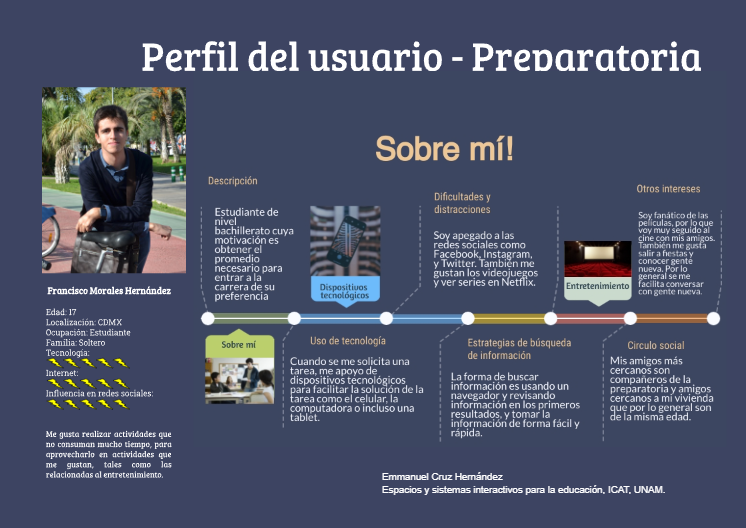
\includegraphics[width=0.60\textwidth]{Cap4/Figuras/Prepa.png}
  \caption{Modelo Persona de alumnos de bachillerato.}
  \label{fig:413}
\end{figure}

Por otro lado, se realizó un modelo Persona enfocado a estudiantes de primeros semestres de licenciatura. Este modelo es el resultado de la recopilación de datos de las actividades realizadas con los alumnos de primeros semestres de la facultad de ciencias.

En el modelo Persona de la Figura \ref{fig:414} se presenta a Abraham, un estudiante de licenciatura de 20 años, con agilidad para manejar diferentes herramientas en Internet, pero a diferencia de Francisco, por el consumo de tiempo de su carrera, no tiene mucha influencia en las redes sociales. Abraham se siente atraído e interesado por conocer nuevos lugares y aprender nuevas cosas con el fin de crecer en el ámbito académico y profesional.

Abraham se siente motivado por terminar su carrera, obtener su título y encontrar un trabajo que le agrade y que cuente con un ambiente en el que se sienta cómodo. Durante su tiempo libre, trata de aprender sobre diferentes temas relacionados al arte, tal como pintura, música o lectura.

Cuando Abraham realiza una investigación, se apoya de diferentes fuentes de información, entre las cuales se encuentran los libros, revistas científicas, bibliotecas virtuales y blogs en la web. Siempre procura obtener la información más confiable y clara, que le permita entender de forma sencilla los temas que busca.

Abraham suele utilizar algunas aplicaciones que le permitan tener un hábito de productividad. Entre las aplicaciones que usa para organizar su tiempo de forma flexible, se encuentran Trello, Slack y Asana.

Algunos intereses de Abraham son las series de género dramático y suspenso. Por lo general utiliza la plataforma Netflix.

\begin{figure}[H]
% \begin{figure}
  \centering
  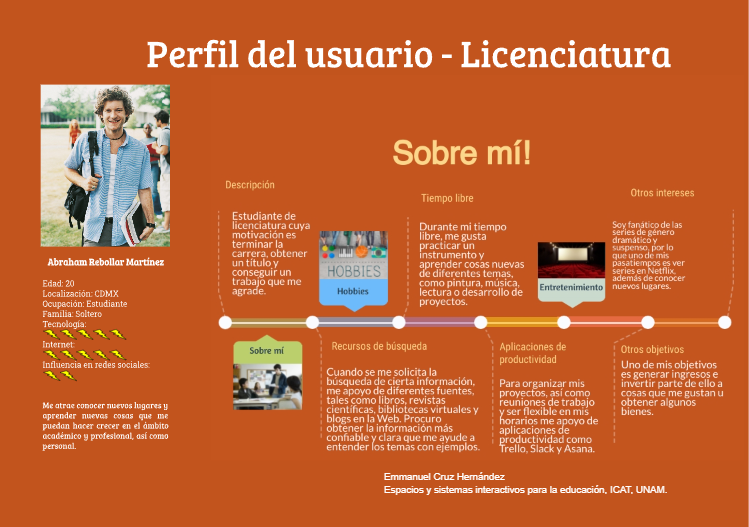
\includegraphics[width=0.60\textwidth]{Cap4/Figuras/Lic.png}
  \caption{Modelo Persona de alumnos de primeros semestres de licenciatura.}
  \label{fig:414}
\end{figure}

%------------------------------------------------------------
%	Diseño de Customer Journey Map para la skill
%------------------------------------------------------------

\subsection{Diseño de Customer Journey Map para la skill}
\label{DisenioCustomerJourneyMapSkillcapIV}

Con el fin de facilitar la comprensión de cómo se comportan los usuarios de forma general en diferentes contextos, se realizó un Customer Journey Map, que muestra los puntos generales que realizan los alumnos para completar una actividad.

En cada punto del proceso de investigación de información, se analizan sus acciones, objetivos, pensamientos, emociones y oportunidades. En la Figura \ref{fig:415} se muestra el flujo representado por un Customer Journey Map.

\begin{figure}[H]
% \begin{figure}
  \centering
  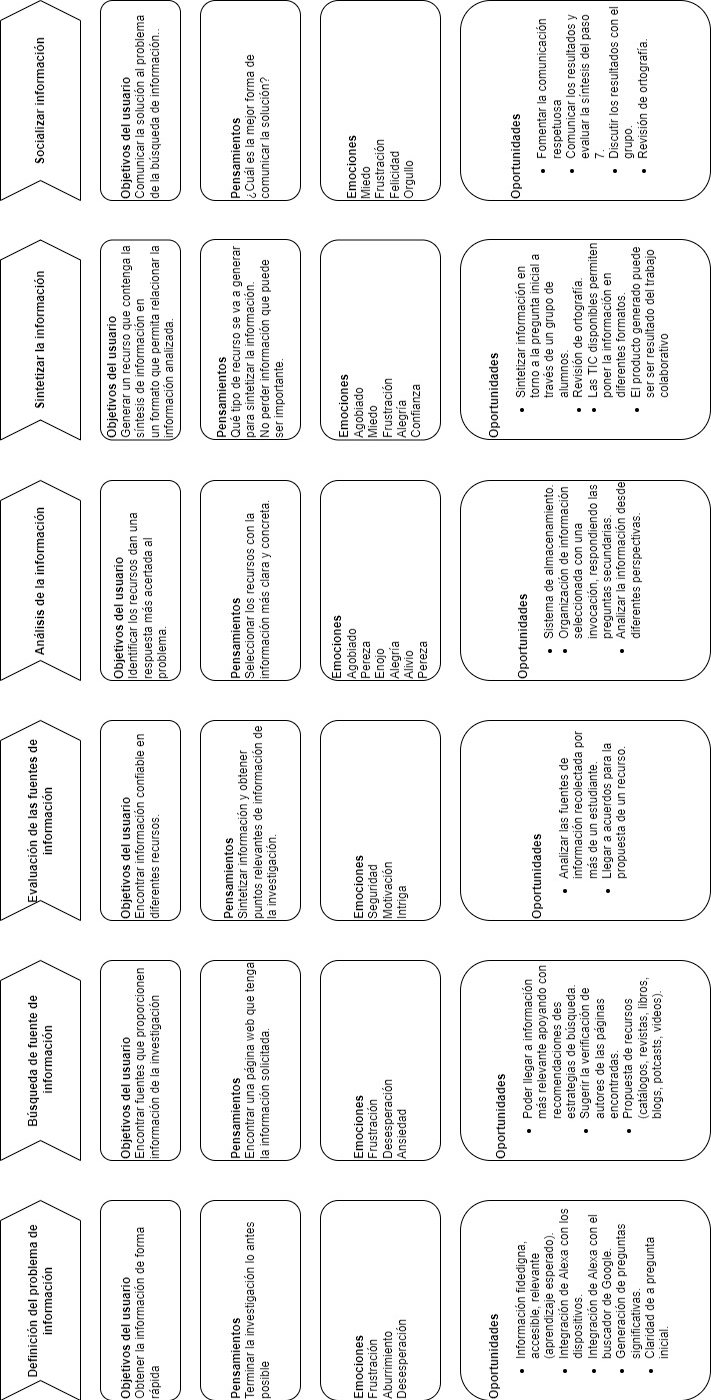
\includegraphics[width=0.60\textwidth]{Cap4/Figuras/Customer Journey Map Skill Rotada.png}
  \caption{Customer Journey Map del proceso de búsqueda de información de los alumnos.}
  \label{fig:415}
\end{figure}

El Customer Journey Map se divide en seis pasos o fases principales:

\begin{enumerate}
  \item Definición del problema de información.
  \item Búsqueda de fuente de información.
  \item Evaluación de las fuentes de información.
  \item Análisis de la información.
  \item Sintetizar la información.
  \item Socializar información.
\end{enumerate}

%------------------------------------------------------------
%	Adaptación del Modelo Gavilán
%------------------------------------------------------------

\subsection{Adaptación del Modelo Gavilán}
\label{AdaptacionModeloGavilancapIV}

A partir de la información obtenida en cada una de las etapas del Customer Journey Map, se obtuvieron oportunidades a considerar para el diseño de la skill, las cuales están enfocadas al entorno de la consola de desarrollo de Alexa. En cada etapa se obtuvieron las siguientes oportunidades.

\begin{itemize}
  \item Definición del problema de información
  \begin{itemize}
    \item Apoyar con la generación de una pregunta inicial y preguntas secundarias.
  \end{itemize}
  \item Búsqueda de fuente de información
  \begin{itemize}
    \item Dar prioridad a las fuentes de información provenientes de una institución educativa.
  \end{itemize}
  \item Evaluación de las fuentes de información
  \begin{itemize}
    \item Permitir al usuario elegir la fuente de información donde investigar.
  \end{itemize}
  \item Análisis de la información
  \begin{itemize}
    \item Almacenar información seleccionada en una estructura de datos por medio de una invocación de la skill.
  \end{itemize}
  \item Sintetizar la información
  \begin{itemize}
    \item Diseñar un mecanismo para recordar el nombre de la tarea, las fuentes consultadas y la fecha de entrega.
  \end{itemize}
  \item Socializar información
  \begin{itemize}
    \item Decir la información final de la investigación recopilada con la skill.
    \item Sugerir estrategias para compartir la información (modelos para comunicar la información).
  \end{itemize}
\end{itemize}

A partir de los puntos anteriores, se diseñó una adaptación en la que el Modelo Gavilán se puede acoplar de la forma más satisfactoria para cubrir las oportunidades enfocadas al desarrollo de la skill. Cabe mencionar que el Modelo Gavilán es un modelo que define sus pasos como guía para seguir un proceso de investigación de información, sin embargo, este puede ser adaptado a las necesidades del problema para ser aplicado de la forma más conveniente.

La adaptación del Modelo Gavilán se conforma a partir de los siguientes pasos, subpasos y objetivos:

\begin{enumerate}
  \item \textbf{Definición del problema de investigación.}
  \begin{enumerate}[1.]
    \item \textbf{Sugerir una pregunta inicial y analizarla.} La skill podrá crear un listado de sugerencias de preguntas relacionadas al tema de la investigación. En esta etapa el usuario podrá comenzar la investigación con la pregunta inicial que le parezca más adecuada a sus objetivos.
    \item \textbf{Elegir la construcción de un plan de investigación.} A partir de la selección de una pregunta, el usuario comienza a crear un plan de construcción con la limitación de un tema general en un subtema.
    \item \textbf{Sugerir preguntas secundarias.} Las preguntas sugeridas por la skill, que no fueron elegidas como pregunta inicial, fungen como preguntas secundarias, que abordan subtemas alternos al principal.
  \end{enumerate}
  \item \textbf{Búsqueda y evaluación de fuentes de información.}
  \begin{enumerate}[1.]
    \item \textbf{Identificar y seleccionar las fuentes de información más adecuadas.} La skill tendrá la capacidad de sugerir diferentes fuentes de información de distintas páginas en la web. Antes de extraer información, proporciona las fuentes de información para que el usuario analice y determine cuáles son las más adecuadas para la investigación.
    \item \textbf{Acceder a las fuentes de información seleccionadas.} Una vez elegida una fuente de información, la skill podrá proporcionar información específica sobre el contenido de la fuente.
    \item \textbf{Evaluar las fuentes de información encontradas.} El usuario podrá escuchar por medio de la skill, la información para poder analizarla y determinar si el contenido es útil para la investigación final.
  \end{enumerate}
  \item \textbf{Análisis de la información.}
  \begin{enumerate}[1.]
    \item \textbf{Elegir la información más adecuada para responder las preguntas secundarias.} El usuario podrá recolectar información que permita responder de manera directa a puntos específicos de un tema o subtema. La skill proporcionará un mecanismo de almacenamiento de fragmentos de información que responde a preguntas secundarias.
    \item \textbf{Leer, entender, comparar y evaluar la información seleccionada para responder las preguntas secundarias.} La información recopilada podrá ser consultada en cualquier momento desde la skill, con el fin de comparar y evaluar el contenido de la investigación.
  \end{enumerate}
  \item \textbf{Síntesis y socialización de la información.}
  \begin{enumerate}[1.]
    \item \textbf{Responder la pregunta inicial.} Cuando se termina el proceso de investigación con el apoyo de la skill, ésta enviará las fuentes de información a un dispositivo móvil, que en conjunto responderá a la pregunta inicial.
    \item \textbf{Elaborar un producto concreto y comunicar los resultados de la investigación.} La skill proporciona un mecanismo para seguir una estrategia de búsqueda de información, sin embargo, no elabora un producto final. La skill podrá sugerir diferentes modelos y estrategias para representar la información consultada.
  \end{enumerate}
\end{enumerate}

%------------------------------------------------------------
%	Diseño de la skill
%------------------------------------------------------------

\section{Diseño de la skill}
\label{DisenioSkillcapIV}

A partir de los resultados obtenidos con las herramientas creadas en la etapa del análisis del usuario y la adaptación del Modelo Gavilán, se crearon herramientas para facilitar el diseño de la skill.

La primera herramienta de apoyo para conocer la interacción de la skill con un usuario, considerando la adaptación del Modelo Gavilán, fue una recopilación de imágenes que forman un Storyboard.

Posteriormente, se diseñó un esquema para definir la navegación de la skill. Esta herramienta considera el flujo de la forma de interacción de un usuario con la skill mostrado en el Storyboard.

%------------------------------------------------------------
%	Storyboard
%------------------------------------------------------------

\subsection{Storyboard}
\label{StoryboardcapIV}

% REFERENCIA
La fundación de interacción de diseño (2022c) señala que es posible crear un guión gráfico con cada uno de los pasos de un proceso. Cada una de las imágenes muestra el proceso de alguna actividad para tener una mejor visión de cómo un usuario puede interactuar con un producto o servicio, a este conjunto de imágenes se conoce como storyboard.

Antes de comenzar con la implementación, se creó un storyboard para visualizar de una forma más clara la forma de interacción, así como los diálogos posibles y las respuestas que podría devolver la skill. A continuación se presentan los cuadros del storyboard de cada uno de los pasos definidos en el Customer Journey Map de la sección \ref{DisenioCustomerJourneyMapSkillcapIV}.

\begin{itemize}
  \item \textbf{Definición del problema de información.} El alumno se muestra frustrado por comenzar una investigación, en este caso, sobre la fotosíntesis. La skill provee un listado de preguntas sugeridas para seleccionar una pregunta inicial y comenzar con la investigación. Este proceso se puede visualizar en la Figura \ref{fig:416}.
  \begin{figure}[H]
  % \begin{figure}
    \centering
    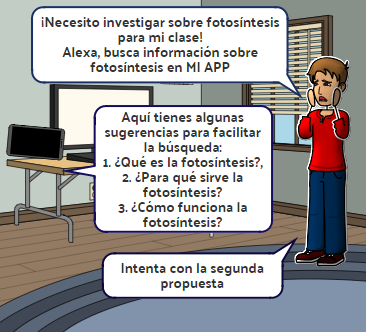
\includegraphics[width=0.40\textwidth]{Cap4/Figuras/01.png}
    \caption{Storyboard, definición del problema de información.}
    \label{fig:416}
  \end{figure}
  \item \textbf{Búsqueda de fuentes de información.} Durante la búsqueda de fuentes de información, se sugieren una serie de fuentes que contienen información relacionada a la pregunta inicial. El usuario analiza las fuentes de información y selecciona la que considera más adecuada. Este proceso se puede consultar en la Figura \ref{fig:417}.
  \begin{figure}[H]
  % \begin{figure}
    \centering
    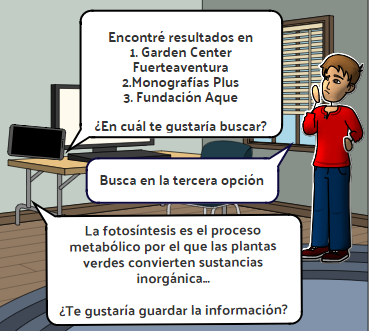
\includegraphics[width=0.40\textwidth]{Cap4/Figuras/02.png}
    \caption{Storyboard, búsqueda de fuentes de información.}
    \label{fig:417}
  \end{figure}
  \item \textbf{Evaluación de las fuentes de información.} Cuando se presenta la información extraída de la fuente seleccionada, el usuario analiza el contenido y determina si es útil para la investigación. En caso de ser útil, el usuario tiene la posibilidad de almacenar el fragmento de información. Este paso se puede visualizar en la Figura \ref{fig:418}.
  \begin{figure}[H]
    \centering
    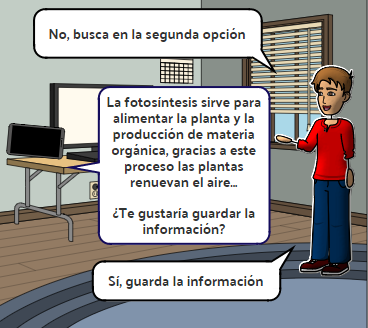
\includegraphics[width=0.40\textwidth]{Cap4/Figuras/03.png}
    \caption{Storyboard, evaluación de las fuentes de información.}
    \label{fig:418}
  \end{figure}
  \item \textbf{Análisis de la información.} El usuario analiza la información y determina si es necesario incluir más datos que sean útiles para la investigación final. El usuario interactúa con la skill de tal forma que puede consultar más contenido en otras fuentes de información y analizar el contenido hasta que considera que la información que ha obtenido es suficiente. Este paso se puede visualizar en la Figura \ref{fig:419}.
  \begin{figure}[H]
    \centering
    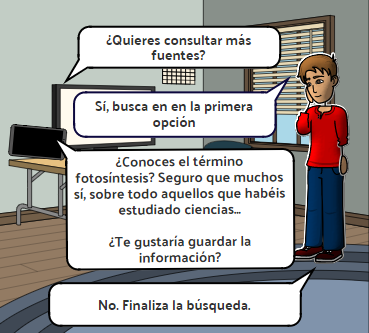
\includegraphics[width=0.40\textwidth]{Cap4/Figuras/04.png}
    \caption{Storyboard, análisis de la información.}
    \label{fig:419}
  \end{figure}
  \item \textbf{Sintetizar la información.} La skill provee una serie de recomendaciones para incluir durante la síntesis de la investigación, tal como las fuentes de información consultadas. Además, aporta un mecanismo de recordatorios para la entrega de una investigación. Este paso se puede visualizar en la Figura \ref{fig:420}.
  \begin{figure}[H]
    \centering
    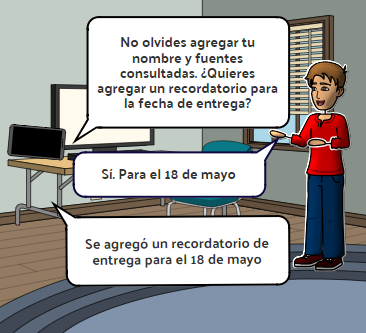
\includegraphics[width=0.40\textwidth]{Cap4/Figuras/07.png}
    \caption{Storyboard, sintetizar la información.}
    \label{fig:420}
  \end{figure}
  \item \textbf{Socializar información.} Finalmente, se dice toda la información recopilada durante el manejo de la skill. Además, la skill proporciona una serie de estrategias para compartir la información y se pueda elaborar un producto final. Este paso se puede visualizar en la Figura \ref{fig:421}.
  \begin{figure}[H]
    \centering
    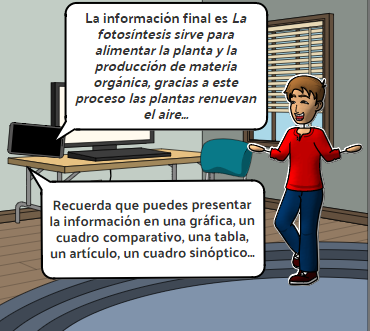
\includegraphics[width=0.40\textwidth]{Cap4/Figuras/06.png}
    \caption{Storyboard, socializar la información.}
    \label{fig:421}
  \end{figure}
\end{itemize}

%------------------------------------------------------------
%	Diagrama de navegación
%------------------------------------------------------------

\subsection{Diagrama de navegación}
\label{DiagramaNavegacioncapIV}

% REFERENCIA
La fundación de interacción de diseño (2022d) señala que un diagrama de flujo o de navegación, son diagramas que permiten visualizar de forma esquemática el flujo de un producto para resolver una tarea o subtarea.

El diagrama de navegación del Buscador Gavilán se divide en cinco secciones principales:

\begin{enumerate}
  \item \textbf{La selección de una pregunta inicial.} Se provee una sugerencia de pregunta inicial. El usuario tiene la opción de elegir o rechazar la pregunta sugerida.
  \begin{itemize}
    \item Si el usuario rechaza la pregunta sugerida, se presenta otra sugerencia y se repite este proceso.
    \item Si el usuario acepta la pregunta inicial sugerida, se pasa a la siguiente sección.
  \end{itemize}
  \item \textbf{La selección de una fuente de información.} La skill presenta una serie de fuentes de información para comenzar a extraer la información. Cada una de las sugerencias se van presentando una a una.
  \begin{itemize}
    \item Si el usuario rechaza la fuente de información sugerida, se presenta otra sugerencia y se repite este proceso.
    \item Si el usuario acepta la fuente de información sugerida, se pasa a la siguiente sección.
  \end{itemize}
  \item \textbf{Extracción, análisis y evaluación de la información.} La skill indaga en el contenido de la fuente de información, diciendo al usuario el contenido dividido en párrafos. Cuando se termina de leer un párrafo, la skill propone dos opciones para continuar el flujo.
  \begin{itemize}
    \item Si el usuario desea saber más contenido de la fuente, lee otro párrafo y realiza el mismo proceso de esta sección, además de tener la posibilidad de almacenar el contenido.
    \item Si el usuario prefiere seguir con el flujo, se da la posibilidad de indagar en más fuentes de información, regresando a la sección dos, o terminar con la investigación, pasando a la siguiente sección.
  \end{itemize}
  \item \textbf{Síntesis de la información.} La skill proporciona una serie de recomendaciones para incluir en el trabajo final, tal como el nombre y las fuentes de información. Además, da la posibilidad de agregar un recordatorio para la fecha de entrega. Si el usuario agrega u omite el recordatorio, ambos flujos pasan a la siguiente sección.
  \item \textbf{Socialización de la información.} En esta última sección se da un resumen del contenido extraído durante la búsqueda, así como el envío de las fuentes de información a la aplicación móvil de Alexa para indagar más en las fuentes originales.
\end{enumerate}

A continuación, se presenta el diagrama de navegación general de la skill en la Figura \ref{fig:422}, donde los diálogos en azul corresponden a la interacción del usuario, los diálogos en verde representan las respuestas de la skill y los apartados en blanco corresponde al inicio y término de ejecución de la skill.

\begin{figure}[H]
  \centering
  \includegraphics[width=0.90\textwidth]{Cap4/Figuras/DiagramaDeNavegación.png}
  \caption{Storyboard, socializar la información.}
  \label{fig:422}
\end{figure}

%------------------------------------------------------------
%	Implementación
%------------------------------------------------------------

\section{Implementación}
\label{ImplementacioncapIV}

Dado el análisis del problema, el análisis del usuario y las herramientas proporcionadas en la etapa de diseño, se implementó una skill llamada Buscador Gavilán, que tiene como objetivo abordar el problema encontrado en el análisis del problema. El logo de la skill se presenta en la Figura \ref{fig:423}.

\begin{figure}[H]
  \centering
  
\includegraphics[width=0.40\textwidth]{Cap4/Figuras/LogoSkill.png}
  \caption{Logo del Buscador Gavilán.}
  \label{fig:423}
\end{figure}

La skill funge como un apoyo para la búsqueda de información, en la que se guía a un usuario a realizar una búsqueda, basada en la adaptación de los cuatro pasos definidos en el Modelo Gavilán: definición del problema de información, búsqueda de fuente de información, evaluación de las fuentes de información y análisis de la información.

A partir de las herramientas construidas en la etapa de análisis del usuario, se crearon herramientas para el diseño de la skill. En particular, el diseño de la skill se basa en el diagrama de navegación para la construcción del flujo de interacción con el usuario.

%------------------------------------------------------------
%	Invocaciones del Buscador Gavilán
%------------------------------------------------------------

\subsection{Invocaciones del Buscador Gavilán}
\label{InvocacionesBuscadorGavilancapIV}

El Buscador Gavilán es una skill que entra en la categoría de skills personalizadas, por lo que requiere un nombre de invocación. El comando de invocación de una skill es la forma en que se solicita la llamada de la misma para comenzar a ejecutar su funcionamiento.

La skill Buscador Gavilán reconoce dos tipos de invocaciones: invocaciones sin solicitud e invocación solicitada sólo por nombre, tal como se muestra en los siguientes ejemplos:

\begin{itemize}
  \item Alexa, abre Buscador Gavilán - invocación sin solicitud
  \item Alexa, comienza Buscador Gavilán - invocación sin solicitud
  \item Alexa, Buscador Gavilán - invocación solicitada sólo por nombre
\end{itemize}

Es importante mencionar que el nombre de invocación de la skill siempre va seguido de la palabra de activación “Alexa”. Dependiendo de la configuración del nombre de activación del dispositivo, este podría usar como palabras de activación “Echo” o “Amazon”.

Es importante mencionar que el nombre de invocación considera la entonación del usuario, por lo que el acento incorporado en el nombre de la skill es reconocido por los dispositivos con Alexa integrada.

%------------------------------------------------------------
%	Intenciones, declaraciones y slots del Buscador Gavilán
%------------------------------------------------------------

\subsection{Intenciones, declaraciones y slots del Buscador Gavilán}
\label{IntencionesDeclaracionesSlotscapIV}

Las intenciones de la skill cuentan con conjunto de declaraciones cada una. A su vez, algunas declaraciones cuentan con uno o más slots. Cada intención de la skill está diseñada para resolver una subtarea específica del problema general en cada proceso de la búsqueda de información con el Buscador Gavilán. A continuación se presentan las intenciones reconocidas por la skill y la subtarea que resuelve, así como las declaraciones y slots utilizados.

%------------------------------------------------------------
%	AMAZON.CancelIntent
%------------------------------------------------------------

\subsubsection{AMAZON.CancelIntent}
\label{CancelIntentcapIV}

Esta intención se encuentra predefinida por la consola de desarrollo de Alexa como una intención requerida, por lo que no puede ser eliminada. Su objetivo es englobar todas las declaraciones para terminar la ejecución de una subtarea, sin salir de la skill.

Al ser una intención que está definida por omisión, las declaraciones se encuentran predefinidas con la misma. Entre las declaraciones posibles para invocar la intención se encuentran las siguientes palabras y frases:

\begin{itemize}
  \item Cancelar
  \item Cancela
\end{itemize}

%------------------------------------------------------------
%	AMAZON.HelpIntent
%------------------------------------------------------------

\subsubsection{AMAZON.HelpIntent}
\label{HelpIntentcapIV}

Esta intención se encuentra predefinida por la consola de desarrollo de Alexa como una intención requerida, por lo que no puede ser eliminada. Está enfocada a englobar las declaraciones que sirven como guía al usuario, brindando instrucciones de ayuda para poder utilizar la skill.

Entre las declaraciones posibles para invocar la intención se encuentran las siguientes:

\begin{itemize}
  \item Ayuda
  \item Quiero ayuda
\end{itemize}

%------------------------------------------------------------
%	AMAZON.StopIntent
%------------------------------------------------------------

\subsubsection{AMAZON.StopIntent}
\label{StopIntentcapIV}

Esta intención se encuentra predefinida por la consola de desarrollo de Alexa como una intención requerida, por lo que no puede ser eliminada. A diferencia de la intención AMAZON.CancelIntent, esta intención engloba las declaraciones para terminar la ejecución completa de la skill.

Entre las declaraciones posibles para invocar la intención se encuentran las siguientes palabras y frases:

\begin{itemize}
  \item Para
  \item Termina
  \item Cierra skill
  \item Cierra la skill
\end{itemize}

%------------------------------------------------------------
%	AMAZON.NavigateHomeIntent
%------------------------------------------------------------

\subsubsection{AMAZON.NavigateHomeIntent}
\label{NavigateHomeIntentcapIV}

Esta intención se encuentra predefinida por la consola de desarrollo de Alexa como una intención requerida, por lo que no puede ser eliminada, sin embargo, esta intención está configurada para funcionar únicamente con dispositivos que cuentan con pantalla.

Su función es cerrar la skill y posicionar la vista de la pantalla en la pantalla de inicio de Alexa. La intención puede ser invocada por medio de las siguientes declaraciones:

\begin{itemize}
  \item Ve al inicio
  \item Inicio
\end{itemize}

%------------------------------------------------------------
%	AMAZON.FallbackIntent
%------------------------------------------------------------

\subsubsection{AMAZON.FallbackIntent}
\label{FallbackIntentcapIV}

Esta intención se encuentra predefinida por la consola de desarrollo de Alexa como una intención requerida, por lo que no puede ser eliminada. Su función es englobar las declaraciones que dan orientación al usuario cuando alguna solicitud no fue reconocida por las declaraciones válidas de cualquier intención.

Esta intención no cuenta con declaraciones predefinidas, ya que se invoca únicamente en caso de no reconocer la solicitud con alguna declaración válida.

%------------------------------------------------------------
%	tellTopicIntent
%------------------------------------------------------------

\subsubsection{tellTopicIntent}
\label{tellTopicIntentcapIV}

Es una intención personalizada que tiene como objetivo englobar las declaraciones que obtienen el tema general de la investigación. Esta intención es el comienzo del flujo de interacción con la skill, en donde es necesario conocer el tema del cual se buscará información.

Dada la gran variedad de formas en que se puede solicitar información de un tema, se crearon sesenta y siete declaraciones, entre las que se encuentran las siguientes:

\begin{itemize}
  \item dime sobre el tema de \{searchWord\}
  \item dame el tema \{searchWord\}
  \item quiero saber sobre el tema de \{searchWord\}
  \item quiero saber sobre el tema \{searchWord\}
  \item sobre el tema \{searchWord\}
  \item por qué \{searchWord\}
  \item donde puedo \{searchWord\}
  \item donde fue la \{searchWord\}
  \item cuando fue el \{searchWord\}
  \item cómo funciona la \{searchWord\}
  \item que es el \{searchWord\}
  \item debo investigar acerca de \{searchWord\}
  \item dime de \{searchWord\}
  \item busca sobre \{searchWord\}
\end{itemize}

Cada una de las declaraciones definidas anteriormente cuenta con un slot, llamado \textit{searchWord}. Este slot es la variable que almacena en texto el tema con el que se comenzará la investigación.

El slot \textit{searchWord} es de tipo AMAZON.SearchQuery, el cual convierte la información en una palabra o frase que puede ser ingresada en un motor de búsqueda estándar. Dado que la búsqueda de información se basa en la web, este tipo de slot es el más adecuado para obtener la información acerca del tema general de la investigación.

%------------------------------------------------------------
%	AMAZON.YesIntent
%------------------------------------------------------------

\subsubsection{AMAZON.YesIntent}
\label{YesIntentcapIV}

Esta intención se encuentra predefinida por la consola de desarrollo de Alexa como una intención no requerida u opcional. Su función es englobar todas las declaraciones para reconocer aquellas entradas que pueden ser consideradas como una afirmación. En la skill, se utiliza para reconocer declaraciones que confirman una pregunta inicial o una fuente de información a investigar.

Dado que la intención es predefinida, algunas declaraciones ya se encuentran incorporadas por omisión,tales como las siguientes:

\begin{itemize}
  \item Sí
  \item Confirmo
  \item Afirmativo
  \item Así es
  \item Es correcto
\end{itemize}

A su vez, se incorporaron otras declaraciones acordes a la skill para ser reconocidas con el mismo propósito de las declaraciones ya existentes. Entre estas declaraciones personalizadas se encuentran las siguientes:

\begin{itemize}
  \item usa esa sugerencia
  \item quiero esa recomendación
  \item elige la referencia
  \item consulta la referencia
  \item utiliza la pregunta
  \item consulta esa referencia
  \item quiero comenzar por esa opción
  \item sí es la opción
\end{itemize}

%------------------------------------------------------------
%	AMAZON.NoIntent
%------------------------------------------------------------

\subsubsection{AMAZON.NoIntent}
\label{NoIntentcapIV}

Esta intención se encuentra predefinida por la consola de desarrollo de Alexa como una intención no requerida u opcional. Su función es englobar todas las declaraciones para reconocer aquellas entradas que pueden ser consideradas como una negación. En la skill, esta intención es utilizada para reconocer declaraciones para sugerir una pregunta inicial al rechazar una propuesta, o dar una sugerencia de una fuente de información al ser rechazada una propuesta.

Dado que la intención es predefinida, algunas declaraciones ya se encuentran incorporadas por omisión, entre las que se encuentran las siguientes:

\begin{itemize}
  \item No
  \item Estoy en desacuerdo
  \item No es
  \item Negativo
\end{itemize}

Al igual que la intención AMAZON.YesIntent, se incorporaron otras declaraciones acordes a la skill para ser reconocidas con el mismo propósito de las declaraciones ya existentes. Entre estas declaraciones personalizadas se encuentran las siguientes:

\begin{itemize}
  \item sugiere otra pregunta inicial
  \item dame otra pregunta
  \item dame más recomendaciones
  \item dame más sugerencias
  \item busca otra recomendación
  \item busca más
  \item recomiendame otra referencia
  \item consulta más fuentes
  \item busca otra opción
  \item siguiente opción
  \item intenta con otra
\end{itemize}

%------------------------------------------------------------
%	nextInfoIntent
%------------------------------------------------------------

\subsubsection{nextInfoIntent}
\label{nextInfoIntentcapIV}

Es una intención personalizada que tiene el propósito de englobar todas las declaraciones enfocadas a obtener más información de un recurso. Cuando un usuario indaga en el contenido de una fuente de información, esta se presenta por párrafos. Las declaraciones englobadas en ésta intención están enfocadas a obtener el contenido del párrafo siguiente del actual, dentro de la fuente de información elegida.

Las declaraciones definidas para esta intención son las siguientes:

\begin{itemize}
  \item dime más sobre el tema
  \item dime más
  \item quiero más información
  \item dame más información
  \item más información
  \item dime el siguiente
  \item lee siguiente
  \item lee el siguiente párrafo
  \item extiende la información
  \item quiero saber más
  \item siguiente párrafo
\end{itemize}

%------------------------------------------------------------
%	continueIntent
%------------------------------------------------------------

\subsubsection{continueIntent}
\label{continueIntentcapIV}

Es una intención personalizada que tiene el propósito de englobar todas las declaraciones enfocadas a dar la posibilidad de terminar la investigación del contenido de la fuente actual.

Entre las declaraciones definidas en esta intención se encuentran las siguientes:

\begin{itemize}
  \item ir al siguiente paso de la investigación
  \item ir al siguiente paso
  \item sigue la investigación
  \item continuar con la investigación
\end{itemize}

%------------------------------------------------------------
%	endInvestigationIntent
%------------------------------------------------------------

\subsubsection{endInvestigationIntent}
\label{endInvestigationIntentcapIV}

Es una intención personalizada que tiene el propósito de englobar todas las declaraciones enfocadas a terminar la etapa de búsqueda de información, por lo que termina de recomendar fuentes de información y leer contenido de las mismas.

Entre las declaraciones definidas para invocar esta intención se encuentran las siguientes:

\begin{itemize}
  \item concluye la investigación
  \item finaliza la investigación
  \item termina la investigación
\end{itemize}

%------------------------------------------------------------
%	addReminderIntent
%------------------------------------------------------------

\subsubsection{addReminderIntent}
\label{addReminderIntentcapIV}

Es una intención personalizada que tiene el propósito de englobar todas las declaraciones que permiten agregar un recordatorio dentro del sistema de la skill.

Algunas declaraciones definidas para esta intención son las siguientes:

\begin{itemize}
  \item agrega el recordatorio para el día \{date\}
  \item crea el recordatorio para el día \{date\}
  \item agrega el recordatorio para el \{date\}
  \item agrega un recordatorio el \{date\}
\end{itemize}

En las declaraciones definidas, se utiliza un slot llamado date. Este slot es de tipo AMAZON.DATE, el cual transforma las entradas a fechas en el formato 2022-09-00T9. La creación de un recordatorio en la lista de recordatorios del servicio de Alexa, requiere de un día y un mes de forma obligatoria, por lo que el tipo AMAZON.DATE es el más adecuado para almacenar esta información, ya que contiene la información requerida.

En el conjunto de declaraciones de esta intención, existen declaraciones que no contienen el dato de la fecha como un slot, tales como los siguientes:

\begin{itemize}
  \item crea recordatorio
  \item agrega recordatorio
\end{itemize}

El slot llamado \textit{date}, está configurado como un slot obligatorio. Cuando alguna de las declaraciones que no contienen el slot es conocido, la intención realiza solicitudes extra para obtener la fecha. Algunas de las solicitudes realizadas por esta intención son las siguientes.

\begin{itemize}
  \item Dime la fecha de entrega de tu tarea
  \item Dime la fecha en que te recordaré la entrega
  \item ¿Cuándo te lo recuerdo?
  \item ¿Qué día quieres que te recuerde la entrega?
\end{itemize}

Las respuestas válidas a estas solicitudes son las siguientes:

\begin{itemize}
  \item para el \{date\}
  \item para \{date\}
  \item crea un recordatorio para \{date\}
  \item agrega recordatorio para \{date\}
  \item agrega el recordatorio el \{date\}
\end{itemize}

En estas solicitudes se pide el dato \textit{date} obligatoriamente para poder invocar correctamente esta intención.

%------------------------------------------------------------
%	omitIntent
%------------------------------------------------------------

\subsubsection{omitIntent}
\label{omitIntentcapIV}

Es una intención personalizada que tiene el propósito de englobar todas las declaraciones que omiten la declaración de un recordatorio. Dado que los recordatorios fungen como una funcionalidad no obligatoria, es posible saltarlos cuando se reconoce alguna de las declaraciones definidas para esta intención. Entre las que se encuentran las siguientes declaraciones:

\begin{itemize}
  \item omitir recordatorio
  \item omite recordatorio
\end{itemize}

%------------------------------------------------------------
%	lastRequestIntent
%------------------------------------------------------------

\subsubsection{lastRequestIntent}
\label{lastRequestIntentcapIV}

Es una intención personalizada que tiene el propósito de englobar todas las declaraciones que permiten recordar la última solicitud realizada por un usuario. Entre las declaraciones de esta intención se encuentran las siguientes:

\begin{itemize}
  \item Recuérdame la última solicitud
  \item Cuál fue la última solicitud
  \item Dime la última solicitud
  \item Recuérdame la última petición
  \item Recuérdame donde estaba
\end{itemize}

%------------------------------------------------------------
%	Custom Search JSON API
%------------------------------------------------------------

\subsection{Custom Search JSON API}
\label{CustomSearchJSONAPIcapIV}

% REFERENCIA
Google Developers (2022) señala que el API JSON de búsqueda personalizada es un API que permite desarrollar sitios o aplicaciones para buscar y mostrar resultados dados por un motor de búsqueda.

Esta API permite recibir una frase en texto para comenzar la búsqueda. Los resultados encontrados en el motor de búsqueda se devuelven en formato JSON, del cual se puede extraer información de cada resultado, tal como su URL, descripción, dominio, título, lenguaje, entre otros.

Google Developers ofrece el servicio llamado \textit{Custom Search JSON API} con el control de un API Key, que permite identificar un cliente en Google, ya que el API Key está asociada a una cuenta de correo electrónico de Gmail.

A su vez, el API key controla ciertas configuraciones sobre la búsqueda que pueden definirse desde la consola de desarrollo de Google Developers. Algunas de estas configuraciones son restricciones de clave, restricciones de aplicaciones, restricciones de sitios web y restricciones de API.

La construcción básica para obtener los servicios del API JSON de búsqueda personalizada en Python se define de la siguiente forma:

\begin{tcolorbox}[colback=white!25!white,colframe=blue]
  \begin{minted}{python}
from apiclient.discovery import build

api_key = 'API-KEY'
resource = build("customsearch", 'v1', developerKey=api_key).cse()
  \end{minted}
\end{tcolorbox}

Donde API-KEY es la credencial generada por la consola de desarrollo de Google Developers para hacer uso del servicio.

El objeto \textit{resource}, construido en el código anterior, cuenta con un método llamado \textit{list}, el cual permite listar todos los resultados de una página que se mostrarían en un motor de búsqueda convencional como Google, Firefox, Safari, entre otros. La estructura básica para la obtención de resultados desde la API en Python, se muestra a continuación.

\begin{tcolorbox}[colback=white!25!white,colframe=blue]
  \begin{minted}{python}
results = resource.list(q=topic, cx='7931d2f657f7b38a2').execute()
  \end{minted}
\end{tcolorbox}

Donde:

\begin{itemize}
  \item \textbf{q:} corresponde a una palabra o frase que será el tema del que se buscarán resultados en el motor de búsqueda.
  \item \textbf{cx:} corresponde al ID del motor de búsqueda que se usará para realizar la solicitud.
  \item \textbf{results:} es un objeto tipo JSON con la respuesta obtenida de la solicitud. En este objeto se almacenan los resultados encontrados en el motor de búsqueda.
\end{itemize}

%------------------------------------------------------------
%	Generación de preguntas y búsqueda de fuentes
%------------------------------------------------------------

\subsubsection{Generación de preguntas y búsqueda de fuentes}
\label{GeneracionPreguntasBusquedaFuentescapIV}

La generación de preguntas de sugerencia de la skill se apoya del API JSON de búsqueda personalizada para generar sugerencias de preguntas. La forma en que se generan es a partir de la búsqueda de la concatenación de un tema general y las principales palabras que conforman una pregunta, tales como qué, cómo, entre otras.

Cada una de las sugerencias encontradas es filtrada para extraer sólo aquellas apariciones de preguntas, tal como se muestra a continuación.

\begin{tcolorbox}[colback=white!25!white,colframe=blue]
  \begin{minted}{python}
whyQuestion = resource.list(q='por que '+topic,cx='7931d2f657f7b38a2').execute()
whatQuestion = resource.list(q='que '+topic,cx='7931d2f657f7b38a2').execute()
whenQuestion = resource.list(q='cuando '+topic, cx='7931d2f657f7b38a2').execute()
whoQuestion = resource.list(q='quien '+topic, cx='7931d2f657f7b38a2').execute()
howQuestion = resource.list(q='como '+topic, cx='7931d2f657f7b38a2').execute()
  \end{minted}
\end{tcolorbox}

Las variables \textit{whyQuestion}, \textit{whatQuestion}, \textit{whenQuestion}, \textit{whoQuestion} y \textit{howQuestion} contienen una respuesta a los resultados encontrados en el motor de búsqueda, que posteriormente son filtrados por título, donde se verifica que existe un signo de interrogación, el cual denota una pregunta.

Cuando una pregunta es seleccionada como pregunta inicial, se aprovecha el funcionamiento del servicio de búsqueda personalizada para obtener resultados asociados a una pregunta, tal como sigue en el siguiente fragmento de código.

\begin{tcolorbox}[colback=white!25!white,colframe=blue]
  \begin{minted}{python}
resources = resource.list(q=selectedQuestion, cx='7931d2f657f7b38a2').execute()
  \end{minted}
\end{tcolorbox}

Donde:

\begin{itemize}
  \item \textbf{selectedQuestion:} corresponde a una pregunta seleccionada del conjunto de preguntas sugeridas.
  \item \textbf{resources:} contiene los resultados de la búsqueda que fungen como fuentes de información para la skill.
\end{itemize}

%------------------------------------------------------------
%	Web Scraping
%------------------------------------------------------------

\subsection{Web Scraping}
\label{WebScrapingcapIV}

% REFERENCIA
De acuerdo con Bo (2017), el Web Scraping es una técnica para extraer datos de la World Wide Web (www). La información que se puede extraer de la web con la técnica de Web Scraping puede ir desde texto, hasta imágenes y videos. A su vez, permite recopilar grandes cantidades de datos bien organizados en diferentes escenarios que van desde extracciones asistidas por humanos hasta su aplicación en sistemas completamente automatizados.

% REFERENCIA
Bo (2017) señala que el Web Scraping se puede dividir en dos pasos secuenciales: adquirir los recursos web y extraer la información de los datos adquiridos. La técnica para llevar a cabo el primer paso, requiere de una solicitud de tipo HTTP, la cual se forma por una solicitud GET con la URL de la dirección web donde se extraerán los datos. Posteriormente, el proceso de extracción analiza, formatea y organiza los datos en un formato estructurado dentro un objeto de tipo JSON.

Cabe mencionar que aunque el Web Scraping es una técnica poderosa para recopilar grandes cantidades de datos, es importante configurar y programar su funcionamiento de forma ética y responsable. Es decir, la extracción de datos debe considerar cuestiones legales, tales como los derechos de autor, los términos de servicios y el traspaso de bienes muebles, por lo que se vuelve relevante considerar un control responsable sobre el envío de solicitudes para la adquisición de datos, así como dar crédito a los autores. Algunos sitios web cuentan con mecanismos que previenen el ataque de sistemas malignos contra un servidor, por lo que es posible que la técnica de Web Scraping no pueda extraer información de dichos sitios web.

Para el presente proyecto, se implementó un web scraper con el fin de extraer la información de las fuentes de información encontradas en la web con la biblioteca BeautifulSoup, disponible para el lenguaje de programación Python.

En la clase WebScraper se implementan algunos métodos que facilitan el manejo de Web Scraping sobre un sitio web que contenga texto. Estos métodos se definen como se muestra en el siguiente código del anexo \ref{A1Anexo}.

%------------------------------------------------------------
%	Handlers
%------------------------------------------------------------

\subsection{Handlers}
\label{HandlerscapIV}

Los Handlers son funciones que implementan el comportamiento específico para una intención. Los Handlers permiten la construcción de la respuesta de una declaración asociada a la activación de una intención.

A continuación se presentan los Handlers implementados para el Buscador Gavilán y su función general.

\begin{itemize}
  \item \textbf{LaunchRequestHandler.} Implementa el handler con solicitud de tipo LaunchRequest, el cual se ejecuta una vez que se activa la skill. Este lanza un mensaje de bienvenida y una instrucción general de cómo comenzar una investigación con el Buscador Gavilán, tal como se muestra en el anexo \ref{A2Anexo}.
  \item \textbf{CancelOrStopIntentHandler.} Implementa el comportamiento definido para las intenciones AMAZON.CancelIntent y AMAZON.StopIntent, la cual lanza un mensaje de despedida al usuario antes de finalizar la ejecución de la skill, tal como se muestra en el anexo \ref{A3Anexo}.
  \item \textbf{HelpIntentHandler.} Implementa el comportamiento para la intención AMAZON.HelpIntent, la cual lanza una indicación de ayuda dependiendo del estado de la skill. Es decir, puede ayudar a iniciar una investigación, elegir alguna referencia, entre otros. Así mismo, regresa una frase con la última respuesta dada por la skill, tal como se muestra en el anexo \ref{A4Anexo}.
  \item \textbf{FallbackIntentHandler.} Implementa el comportamiento para la intención AMAZON.FallbackIntent, la cual se lanza cuando un comando no es reconocido por las declaraciones de las intenciones válidas. Lanza un mensaje para informar que la solicitud no fue entendida y se vuelva a repetir, así como comunicar la información de la última petición solicitada, tal como se muestra en el anexo \ref{A5Anexo}.
  \item \textbf{tellTopicIntentHandler.} Implementa el comportamiento de la intención tellTopicIntent. Este handler inicializa todos los valores al primer estado, ya que es la primera intención que se ejecuta al comenzar una nueva investigación en la skill. Por otra parte, se crea una nueva instancia de un scraper para comenzar con la generación de preguntas, las cuales se almacenan de forma global durante la ejecución de la skill. Lanza como respuesta una breve información sobre una pregunta inicial y la primera sugerencia de una pregunta, tal como se muestra en el anexo \ref{A6Anexo}.
  \item \textbf{yesAmazonIntentHandler.} Implementa el comportamiento de la intención AMAZON.YesIntent, la cual recibe una respuesta afirmativa. Este handler funciona para dos estados distintos de la skill: cuando se afirma una pregunta inicial y cuando se afirma una fuente de información. Cuando se afirma una pregunta inicial, se lee la pregunta elegida y se da la primera sugerencia de fuente de información relacionada a la pregunta. Cuando se afirma una fuente de información, se lee el autor del dominio del cual se extrae la información y se da conocimiento del primer párrafo de la fuente de información seleccionada, tal como se muestra en el anexo \ref{A7Anexo}.
  \item \textbf{noAmazonIntentHandler.} Implementa el comportamiento de la intención AMAZON.NoIntent, la cual recibe una declaración negativa. En los estados de la skill se puede negar una pregunta sugerida y una fuente de información, por lo que se divide en dos casos dependiendo del estado de la skill. Cuando se niega una pregunta sugerida, se lanza como respuesta otra pregunta sugerida, mientras que cuando se niega una fuente de información, se lanza como respuesta la siguiente fuente de información posible, tal como se muestra en el anexo \ref{A8Anexo}.
  \item \textbf{nextInfoIntentHandler.} Implementa la funcionalidad para la intención nextInfoIntent, la cual lanza como respuesta un párrafo de la fuente de información seleccionada en el proceso de selección de fuentes de información a partir de una pregunta inicial. En caso de no haber leído todos los párrafos, lanza un mensaje informativo para anunciar que no hay más contenido por dar como respuesta, tal como se muestra en el anexo \ref{A9Anexo}.
  \item \textbf{continueIntentHandler.} Implementa la funcionalidad de la intención continueIntent, la cual manda un mensaje informativo para elegir una de dos opciones: consultar más fuentes de información o terminar con el proceso de investigación, tal como se muestra en el anexo \ref{A10Anexo}.
  \item \textbf{endInvestigationIntentHandler.} Implementa la funcionalidad de la intención endInvestigationIntent, la cual da los datos informativos finales de la investigación, tal como consejos generales y una respuesta informativa para agregar u omitir recordatorios, tal como se muestra en el anexo \ref{A11Anexo}.
  \item \textbf{addReminderIntentHandler.} Implementa la funcionalidad para la intención addReminderIntent, la cual permite crear un recordatorio para la fecha de entrega de la investigación, tal como se muestra en el anexo \ref{A12Anexo}.
  \item \textbf{omitIntentHandler.} Implementa la funcionalidad para la intención omitIntent, la cual permite saltar la programación de un recordatorio, dando un resumen sobre la información recopilada durante la investigación, así como dar consejos para crear un producto final con la información recuperada. Este handler finaliza la ejecución de la skill, tal como se muestra en el anexo \ref{A13Anexo}.
  \item \textbf{lastRequestIntentHandler.} Implementa la funcionalidad para la intención lastRequestIntent, la cual permite al usuario saber cuál fue la respuesta de la última solicitud hecha en la skill. Lanza como respuesta la última oración dada por la skill, tal como se muestra en el anexo \ref{A14Anexo}.
\end{itemize}

%------------------------------------------------------------
%	Evaluación de la skill
%------------------------------------------------------------

\section{Evaluación de la skill}
\label{EvaluacionSkillcapIV}

La evaluación es una de las etapas del proceso iterativo del diseño centrado en el usuario, el cual consiste en realizar una serie de pruebas con distintas herramientas, con el fin de identificar los posibles problemas durante el manejo de un producto. Por otra parte, se logran identificar procedimientos, limitaciones y problemas en el diseño. En este apartado se detallan las herramientas usadas para aplicar la evaluación a la skill Buscador Gavilán, así como sus resultados.

%------------------------------------------------------------
%	Herramientas del proceso de evaluación de la skill y pruebas con usuarios
%------------------------------------------------------------

\subsection{Herramientas del proceso de evaluación de la skill y pruebas con usuarios}
\label{HerramientasEvaluacionPruebasUsuarioscapIV}

Para aplicar las pruebas, se toma como base el proceso de evaluación del grupo ESIE con cinco usuarios. Este proceso de evaluación se divide en tres fases principales: en la primera fase, un anfitrión o anfitriones dan la bienvenida a los usuarios y se obtiene información relevante sobre el usuario. A continuación se presentan las herramientas utilizadas en esta etapa:

\begin{itemize}
  \item \textbf{Cuestionario de entrada.} Tiene como propósito, conocer información relacionada a los intereses o tipos de dispositivos que usa el usuario. Esta información resulta útil para conocer la experiencia del usuario frente al funcionamiento de la skill. En el anexo \ref{B1Anexo} se muestra el cuestionario de entrada aplicado.
\end{itemize}

En la segunda fase, uno de los anfitriones lee un protocolo de bienvenida. Posteriormente, indica una serie de actividades que deben ser completadas por los usuarios. Mientras el usuario realiza las pruebas, un observador registra notas y resultados relevantes de cada actividad realizada por los usuarios.

\begin{itemize}
  \item \textbf{Protocolo de bienvenida.} El objetivo de este documento es presentar los objetivos de la evaluación, en este caso, evaluar la usabilidad de la skill Buscador Gavilán. En el anexo \ref{B2Anexo} se puede consultar el protocolo de bienvenida aplicado.
  \item \textbf{Actividades de la prueba.} Es una herramienta que define el listado de actividades que debe realizar un usuario. En el anexo \ref{B3Anexo} se presentan las actividades de la prueba aplicadas.
  \item \textbf{Guión de actividades para la evaluación.} Dada la dificultad para dar a conocer las actividades por voz a través de un anfitrión, las actividades se presentaron en un documento externo, donde se definen las actividades que puede realizar un usuario. En el anexo \ref{B4Anexo} se puede consultar el listado de actividades de la evaluación.
\end{itemize}

En la tercera y última fase de la evaluación, los usuarios responden algunos cuestionarios que permiten conocer la usabilidad y la experiencia al utilizar la skill.

\begin{itemize}
  \item \textbf{Cuestionario de usabilidad.} Este cuestionario contiene reactivos específicos para determinar la usabilidad de la skill Buscador Gavilán. El cuestionario de usabilidad aplicado se muestra en el anexo \ref{B5Anexo}.
  \item \textbf{Cuestionario de percepción subjetiva.} Este cuestionario ayuda a identificar particularidades de la interfaz respecto a la interfaz de usuario. El cuestionario de percepción subjetiva aplicado se muestra en el anexo \ref{B6Anexo}.
\end{itemize}

%------------------------------------------------------------
%	Evaluación con usuarios
%------------------------------------------------------------

\subsection{Evaluación con usuarios}
\label{EvaluacionUsuarioscapIV}

Con el fin de evaluar la usabilidad de la skill Buscador Gavilán de forma virtual, debido al confinamiento del COVID-19, se hicieron algunos ajustes a la aplicación del proceso de evaluación del grupo ESIE, además de ajustarlo para aplicarse a las características de una interfaz basada en reconocimiento por voz.

En el proceso de evaluación del grupo ESIE convencional, el moderador ordena una serie de actividades una a una. Para la evaluación de la skill, el moderador realizó una presentación con todas las funcionalidades posibles de la skill. Esta presentación ayudó a que los usuarios conocieran la interacción con la skill, con el fin de que el moderador no interviniera durante la interacción.

El segundo reto fue adaptar la forma de aplicar la evaluación a una modalidad virtual por medio de una reunión en la plataforma Zoom, en la que se encontraban conectados en línea al menos cuatro dispositivos, cada uno con una funcionalidad específica para poder llevar a cabo la evaluación.

\begin{enumerate}
  \item Un dispositivo con cámara activada para el moderador.
  \item Un dispositivo para el usuario.
  \item Un dispositivo que mostraba en cámara un dispositivo Echo Dot con la skill Buscador Gavilán instalada.
  \item Un dispositivo con cámara desactivada para el observador.
\end{enumerate}

En la Figura \ref{fig:424} se muestra una de las evaluaciones con los usuarios en las que se encuentran los cuatro dispositivos mencionados anteriormente.

\begin{figure}[H]
  \centering
  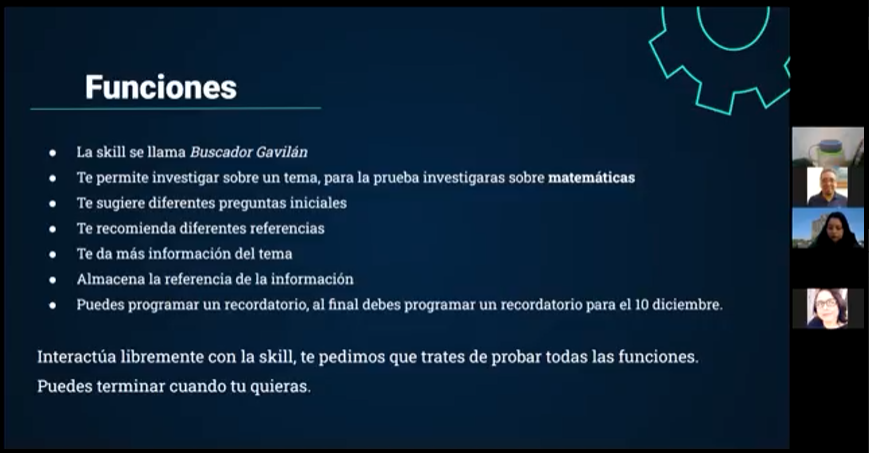
\includegraphics[width=0.70\textwidth]{Cap4/Figuras/Pruebas usuario 1.png}
  \caption{Evaluación de la skill Buscador Gavilán con un usuario.}
  \label{fig:424}
\end{figure}

El proceso de evaluación con cada uno de los usuarios siguió las tres fases principales del proceso de evaluación del grupo ESIE.

En la primera fase, para aplicar el cuestionario de entrada, se envió previamente a la reunión en Zoom, el formulario con los reactivos del cuestionario de entrada por medio de un formulario en Google Forms.

En la segunda fase, se instaló un micrófono y una bocina con el dispositivo Echo Dot, con el fin de tener una mejor transmisión de sonido de entrada y salida en la plataforma Zoom. A su vez, cada una de las reuniones fue grabada con el consentimiento del usuario.

Durante la segunda etapa, el monitor leyó la carta de bienvenida con las reglas a seguir y los objetivos de la evaluación. Posteriormente, el moderador mostró un video a los usuarios, en el que se mostró cómo interactuar con Alexa, así como dar a conocer la definición de una skill y activarlas para ejecutar su funcionamiento. Finalmente, el moderador expuso a los usuarios una presentación con las funciones que la skill puede realizar, en la que se le solicitó interactuar de forma libre, realizando las tareas definidas en el listado de funciones.

Es importante mencionar, que dada la interacción libre de los usuarios con la skill, algunas actividades no fueron realizadas. Finalmente, el observador fue marcando las actividades que fueron realizadas exitosamente, las actividades que trataron de realizarse pero no fueron completadas, y las actividades que no fueron realizadas. Estos resultados se registraron en el documento llamado actividades de la prueba.

Finalmente, en la tercera y última fase del proceso, se solicitó a los usuarios responder los cuestionarios de usabilidad y de percepción subjetiva, la cual cuenta con una sección de comentarios generales sobre la opinión de los usuarios sobre la skill.

%------------------------------------------------------------
%	Resultados y análisis de usabilidad de la skill
%------------------------------------------------------------

\subsection{Resultados y análisis de usabilidad de la skill}
\label{ResultadosAnalisisUsabilidadcapIV}

Los resultados obtenidos de cada una de las herramientas del proceso de evaluación brindan información relevante sobre los usuarios y sobre el manejo de la skill.

%------------------------------------------------------------
%	Cuestionario de entrada
%------------------------------------------------------------

\subsubsection{Cuestionario de entrada}
\label{CuestionarioEntradacapIV}

A continuación se presentan los resultados más relevantes del cuestionario de entrada.

\begin{itemize}
  \item La fuente de información más consultada es la Internet. Todos los usuarios que participaron en la prueba utilizan esta fuente para sus investigaciones.
  \item El 60\% de los usuarios realiza búsquedas de temas de interés personal y el 40\% realiza investigación con propósito académico.
  \item El 40\% de los usuarios casi nunca incluye las referencias utilizadas en la investigación. Otro 40\% sólo las incluye frecuentemente. Algunos usuarios señalan que no agregan las referencias porque el profesor no lo solicita, no lo consideran necesario o porque no es una investigación formal.  
  \item El 60\% de los estudiantes considera que la información que obtienen al final de una investigación es buena.
  \item Las fuentes de información que son más utilizadas por los usuarios son YouTube y Google con un 80\%. Los segundos recursos más utilizados son Wikipedia y revistas científicas con un 60\%.
  \item El 80\% de los usuarios no sigue ningún método de investigación. El usuario que aplica un método de investigación, utiliza el método práctico y teórico aprendido en una clase de sociología.
  \item Por otra parte, el Modelo Gavilán es una estrategia de búsqueda de información que tampoco es conocida por ninguno de los usuarios involucrados.
  \item Todos los usuarios saben qué es un asistente basado en voz. Los asistentes por voz más usados son Google Assistant y Siri, con un 80\%, seguido de Alexa con un 60\%.
  \item A pesar de saber qué son los asistentes basados en voz, sólo el 80\% de los usuarios ha utilizado alguno.
  \item Las funcionalidades más usadas al utilizar un asistente basado en voz se muestran a continuación en la Figura \ref{fig:425}.
  \begin{figure}[H]
    \centering
    \includegraphics[width=0.70\textwidth]{Cap4/Figuras/Funcionalidades más usadas.png}
    \caption{Funcionalidades más usadas al utilizar un asistente basado en voz.}
    \label{fig:425}
  \end{figure}
  \item Ninguno de los usuarios sabe lo que es una skill de Alexa.
  \item Todos los usuarios se sienten cómodos usando un asistente basado en voz.
  \item Todos los usuarios consideran que un asistente basado en voz podría ayudar en el proceso de investigación y búsqueda de información, ya que consideran que podría facilitar las búsquedas en internet, puede recomendar páginas que pueden ser útiles, tienen muchas respuestas, mejoraría la eficiencia en tiempo y podría ser más práctico cuando se están realizando más actividades al mismo tiempo.
\end{itemize}

%------------------------------------------------------------
%	Actividades de la prueba
%------------------------------------------------------------

\subsubsection{Actividades de la prueba}
\label{ActividadesPruebacapIV}

En la tabla siguiente se muestran los resultados de las actividades de la prueba en la Tabla \ref{tab:t43}.

\begin{table}[H]
  \begin{center}
    \begin{tabular}{ | p{7cm} | p{3cm} | p{3cm} | p{3cm} | }
      \hline
       & Usuarios que realizaron la actividad & Usuarios que intentaron realizar la actividad sin éxito & Usuarios que no realizaron la actividad \\ \hline
      Activa la skill & 3 & 2 & 0 \\ \hline
      Solicita a la skill investigar sobre el tema de matemáticas & 1 & 4 & 0 \\ \hline
      Solicita a Alexa que te sugiera una nueva pregunta inicial & 2 & 0 & 3 \\ \hline
      Solicita a Alexa que utilice la pregunta inicial sugerida & 4 & 0 & 1 \\ \hline
      Solicita a Alexa que te recomiende otra referencia & 2 & 1 & 2 \\ \hline
      Solicita a Alexa que utilice la referencia propuesta & 3 & 1 & 1 \\ \hline
      Solicita a la skill más información del tema & 4 & 0 & 1 \\ \hline
      Solicita a la skill buscar otra referencia & 4 & 0 & 1 \\ \hline
      Solicita a Alexa que almacene la referencia de la información & 4 & 0 & 1 \\ \hline
      Solicita a Alexa que continúe con la investigación & 3 & 0 & 1 \\ \hline
      Solicita a Alexa finalizar con la investigación & 2 & 0 & 3 \\ \hline
      Solicita a la skill que programe un recordatorio para el 10 diciembre & 4 & 0 & 1 \\ \hline
    \end{tabular}
    \caption{Resultados de las activiades de la prueba.}
    \label{tab:t43}
  \end{center}
\end{table}

Los resultados obtenidos en las actividades de la prueba se comparan con las hipótesis de cada una de las tareas, en las que se define por cada una la hipótesis, la acción a desarrollar, el tiempo estimado para realizar la tarea y el resultado de la prueba, en donde se define si se cumplió satisfactoriamente o no la hipótesis. Estos resultados se muestran en la Tabla \ref{tab:t44}

\begin{table}[H]
  \begin{center}
    \begin{tabular}{ | p{3cm} | p{3cm} | p{3cm} | p{2cm} | p{4cm} | }
      \hline
      HIPÓTESIS & TAREA & DESARROLLO DE TAREA & TIEMPO ESTIMADO & RESULTADO \\ \hline
      El usuario conoce el comando de activación de la skill. & Activar la skill & Activa la skill & A lo más 20 segundos & Se cumplió la hipótesis \\ \hline
      El usuario es capaz de iniciar la investigación sobre matemáticas & Iniciar la investigación sobre matemáticas & Solicita a la skill investigar sobre el tema de matemáticas & A lo más 50 segundos & Se cumplió la hipótesis pero se identificó que los usuarios intentaron utilizar otras palabras asociadas al intent \\ \hline
      El usuario puede buscar otra propuesta de pregunta inicial & Buscar otra pregunta inicial a la pregunta propuesta & Solicita a Alexa que te sugiera una nueva pregunta inicial & A lo más 40 segundos & Se cumplió la hipótesis. Los intents propuestos no se usaron en las evaluaciones ya que el usuario interactuaba con “si” y “no” \\ \hline
      El usuario acepta la pregunta sugerida para la investigación & Elegir la pregunta propuesta como pregunta inicial para la investigación sobre música & Solicita a Alexa que utilice la pregunta inicial sugerida & A lo más 40 segundos & Se cumplió la hipótesis. Los intents propuestos no se usaron en las evaluaciones ya que el usuario interactuaba con “si” y “no” \\ \hline
      El usuario solicita otra sugerencia para las referencias & Buscar otra referencia propuesta a la primera propuesta por la skill & Solicita a Alexa que te recomiende otra referencia & A lo más 40 segundos & Se cumplió la hipótesis. Los intents propuestos no se usaron en las evaluaciones ya que el usuario interactuaba con “si” y “no” \\ \hline
      El usuario elige una referencia propuesta por la skill & Elegir la referencia propuesta por la skill & Solicita a Alexa que utilice la referencia propuesta & A lo más 40 segundos & Se cumplió la hipótesis. Los intents propuestos no se usaron en las evaluaciones ya que el usuario interactuaba con “si” y “no” \\ \hline
    \end{tabular}
  \end{center}
\end{table}

\begin{table}[H]
  \begin{center}
    \begin{tabular}{ | p{3cm} | p{3cm} | p{3cm} | p{2cm} | p{4cm} | }
      \hline
      El usuario extiende la información de una búsqueda & Solicitar a la skill leer otro párrafo & Solicita a la skill más información del tema & A lo más 40 segundos & 
      Medianamente cumplida. Hay dudas en cómo pedir la extensión de información, no es clara la manera en que se puede formular la solicitud, se esperaba que diera otra información distinta, es parecido a buscar otra pregunta y no queda muy clara la funcionalidad.

      Se propone cambiar la propuesta de extensión de información : Puedes decir “más información” para escuchar más de esta referencia \\ \hline
      El usuario termina la revisión de la referencia actual & Solicitar a la skill seguir consultar otra referencia & Solicita a la skill buscar otra referencia & A lo más 40 segundos & No se cumplió la hipótesis. Hay confusión entre la diferencia de terminar la búsqueda de referencias y la búsqueda de información \\ \hline
      El usuario guarda la referencia de la información investigada & Solicitar a la skill guardar una referencia & Solicita a Alexa que almacene la referencia de la información & A lo más 40 segundos & Se cumplió la hipótesis \\ \hline
      El usuario continúa el proceso de selección de fuentes & Solicitar a la skill continuar con la investigación & Solicita a Alexa que continúe con la investigación & A lo más 40 segundos & No se cumplió la hipótesis. Es confuso el concepto de terminar la investigación y varios de los usuarios no llegan a este punto \\ \hline
    \end{tabular}
  \end{center}
\end{table}

\begin{table}[H]
  \begin{center}
    \begin{tabular}{ | p{3cm} | p{3cm} | p{3cm} | p{2cm} | p{4cm} | }
      \hline
      El usuario finaliza el proceso de selección de fuentes & Solicitar a la skill que termine la investigación & Solicita a Alexa finalizar con la investigación & A lo más 40 segundos & No se cumplió la hipótesis. Este paso se salta y es confusa la diferencia entre terminar la selección de fuentes y terminar la investigación \\ \hline
      El usuario agrega un recordatorio sobre la entrega de la investigación & Solicitar a la skill que agregue un recordatorio & Solicita a la skill que programe un recordatorio para el 10 diciembre & A lo más 40 segundos & Se cumplió medianamente \\ \hline
      El usuario cierra la skill & Solicitar a la skill que se cierre & Solicita a Alexa salir de la skill & A lo más 40 segundos & No se cumplió la hipótesis. Una vez terminada la interacción el usuario ya no sabe qué más hacer y la skill repite la última información dicha hasta que se desactiva automáticamente. \\ \hline
    \end{tabular}
    \caption{Hipótesis y resultados de las actividades de la prueba.}
    \label{tab:t44}
  \end{center}
\end{table}

%------------------------------------------------------------
%	Cuestionario de usabilidad
%------------------------------------------------------------

\subsubsection{Cuestionario de usabilidad}
\label{CuestionarioUsabilidadcapIV}

Los resultados de usabilidad son tomados para aplicar los pasos definidos en el cuestionario de evaluación del cuestionario de usabilidad SUS, en el cual, a los resultados con actitud positiva se les resta una unidad, mientras que a las respuestas con carácter negativo, se le resta el valor obtenido en el cuestionario a cinco.

Realizando el cálculo mencionado anteriormente, se obtuvieron los siguientes resultados por usuarios, mostrado en la Tabla \ref{tab:t45}.

\begin{table}[H]
  \begin{center}
    \begin{tabular}{ | p{9cm} | p{1cm} | p{1cm} | p{1cm} | p{1cm} | p{1cm} | }
      \hline
      \textbf{Pregunta/Número de usuario} & 1 & 2 & 3 & 4 & 5 \\ \hline
      Creo que me gustaría usar la skill frecuentemente & 1 & 3 & 4 & 3 & 4 \\ \hline
      Encuentro la skill compleja & 3 & 2 & 4 & 2 & 3 \\ \hline
      Pienso que la skill es fácil de usar & 0 & 1 & 4 & 3 & 3 \\ \hline
      Creo que necesitaré la ayuda de un técnico para usar la skill & 4 & 4 & 4 & 3 & 4 \\ \hline
      Encontré que las distintas funciones de la skill estaban bien integrados & 2 & 1 & 3 & 3 & 3 \\ \hline
      Pienso que había mucha inconsistencia en la skill & 1 & 2 & 4 & 3 & 3 \\ \hline
      Me imagino que la gente aprenderá a usar la skill bastante rápido & 2 & 4 & 4 & 4 & 4 \\ \hline
      Encuentro la skill engorrosa de usar & 1 & 0 & 4 & 3 & 3 \\ \hline
      Me sentí muy seguro usando la skill & 0 & 1 & 4 & 3 & 4 \\ \hline
      Necesito aprender muchas cosas antes de poder utilizar la skill & 3 & 4 & 4 & 3 & 4 \\ \hline
      Suma & 17 & 22 & 39 & 30 & 35 \\ \hline
      Multiplicación por 2.5 & \textbf{42.5} & \textbf{55} & \textbf{97.5} & \textbf{75} & \textbf{87.5} \\ \hline
    \end{tabular}
    \caption{Resultados del cuestionario de usabilidad.}
    \label{tab:t45}
  \end{center}
\end{table}

La suma de los resultados definidos por SUS, está dada por la siguiente operación:

42.5 + 55 + 97.5 + 75 + 87.5 = 357.5

A este resultado se le obtiene el promedio, que en este caso constó de cinco usuarios:

357.5 / 5 = 71.5

Tomando como referencia la puntuación definida por SUS, este resultado se encuentra en una escala donde la usabilidad de la skill Buscador Gavilán se considera buena.

%------------------------------------------------------------
%	Cuestionario de percepción subjetiva
%------------------------------------------------------------

\subsubsection{Cuestionario de percepción subjetiva}
\label{CuestionarioPercepcionSubjetivacapIV}

Se presentan los resultados en los que se muestra mayor tendencia de los reactivos de percepción subjetiva.

En una escala de 1 (aburrida) a 9 (estimulante), la skill tiende a ser estimulante. Los resultados se ilustran en la Figura \ref{fig:426}.

\begin{figure}[H]
  \centering
  \includegraphics[width=0.70\textwidth]{Cap4/Figuras/PercepciónSubjetiva1.png}
  \caption{Resultados de percepción subjetiva 1.}
  \label{fig:426}
\end{figure}

En una escala de 1 (difícil) a 9 (fácil) para recordar los nombres y funcionalidades de la skill, esta tiende a ser fácil de recordar. Los resultados se ilustran en la Figura \ref{fig:427}.

\begin{figure}[H]
  \centering
  \includegraphics[width=0.70\textwidth]{Cap4/Figuras/PercepciónSubjetiva2.png}
  \caption{Resultados de percepción subjetiva 2.}
  \label{fig:427}
\end{figure}

En una escala de 1 (inadecuada) a 9 (adecuada), la cantidad de ayuda ofrecida por la skill tiende a ser adecuada. Los resultados se ilustran en la Figura \ref{fig:428}.

\begin{figure}[H]
  \centering
  \includegraphics[width=0.70\textwidth]{Cap4/Figuras/PercepciónSubjetiva3.png}
  \caption{Resultados de percepción subjetiva 3.}
  \label{fig:428}
\end{figure}

En una escala de 1 (confusos) a 9 (claros), los mensajes de las instrucciones sobre las actividades que puede realizar una skill tienden a ser claros. Los resultados se ilustran en la Figura \ref{fig:429}.

\begin{figure}[H]
  \centering
  \includegraphics[width=0.70\textwidth]{Cap4/Figuras/PercepciónSubjetiva4.png}
  \caption{Resultados de percepción subjetiva 4.}
  \label{fig:429}
\end{figure}

En una escala de 1 (confusos) a 9 (claros), los mensajes de error tienden a ser claros. Los resultados se ilustran en la Figura \ref{fig:430}.

\begin{figure}[H]
  \centering
  \includegraphics[width=0.70\textwidth]{Cap4/Figuras/PercepciónSubjetiva5.png}
  \caption{Resultados de percepción subjetiva 5.}
  \label{fig:430}
\end{figure}

En una escala de 1 (poco) a 9 (mucho), la skill tiende a ser demasiado innovadora. Los resultados se ilustran en la Figura \ref{fig:431}.

\begin{figure}[H]
  \centering
  \includegraphics[width=0.70\textwidth]{Cap4/Figuras/PercepciónSubjetiva6.png}
  \caption{Resultados de percepción subjetiva 6.}
  \label{fig:431}
\end{figure}

Comentarios de los usuarios sobre la skill:

\begin{itemize}
  \item Que me haga caso.
  \item Skill es fácil de usar una vez que le encuentras la forma, me agrada que sea clara y precisa. Que de sugerencias y busque aprobación de las páginas antes de dar la información de dichas. Lo único que me gustaría es que al detectar errores pudiera decir cómo es que espera la respuesta o por qué surgió el error. De ahí en fuera me agrada el funcionamiento.
  \item Faltaría la traducción de las páginas en inglés para que las diga en español.
  \item Lo único que no supe es que como era que me dejara de dar referencias o ya no continuará leyendo el siguiente párrafo, y cuando hacía un recordatorio, decía sobre un error y luego decía que si estaba el recordatorio.
\end{itemize}

%------------------------------------------------------------
%	Resumen
%------------------------------------------------------------

\section{Resumen}
\label{ResumencapIV}

En este capítulo se describen y presentan los conceptos más generales involucrados en el desarrollo de una skill, tal como el Alexa Skills Kit, que es un conjunto de herramientas para desarrollar skills; la consola de desarrollo de Alexa, la cual brinda un entorno para desarrollar las skills; invocaciones, que son las formas en que se puede activar una skill; las intenciones, que son las funcionalidades que puede realizar una skill; declaraciones, que es un conjunto de frases que pueden invocar una intención;  slots, que fungen como parámetros en las declaraciones para brindar información específica; función lambda, que es el entorno en que se desarrolla todo el código para el funcionamiento de la skill; y el simulador de Alexa, que permite probar la skill de forma interactiva.

Posteriormente, se identifica el problema a tratar a partir del análisis del problema, donde se presentan una serie de problemas del proceso de investigación y búsqueda de información de alumnos de entre 15 y 21 años. Así mismo, se compara el proceso de investigación que realizan los alumnos, con el proceso de búsqueda de información sugerido por las etapas del Modelo Gavilán.

Dada la información encontrada en el proceso de análisis del problema, se realizan herramientas para el diseño de la skill Buscador Gavilán, enfocada a la metodología basada en el diseño centrado en el usuario. Se desarrollaron herramientas como el modelo Persona, el Customer Journey Map y una adaptación del Modelo Gavilán. Estos documentos permiten la creación de herramientas enfocadas al diseño técnico de la skill, tales como un story board y un diagrama de navegación.

Consecutivamente, se describen todos los aspectos considerados durante la implementación de la skill, tal como las invocaciones, intenciones, declaraciones, slots, handlers, entre otros datos como las tecnologías utilizadas como apoyo para el correcto funcionamiento, como el Custom Search JSON API y el Web Scraping.

Finalmente se presenta un apartado donde se muestran las pruebas realizadas con los usuarios y los resultados del proceso de evaluación de usabilidad de la skill. Con esta evaluación se identifican algunos problemas, en los que se propone una solución para mejorar la interacción de la skill con los usuarios.



%------------------------------------------------------------
%	CAPÍTULO V
%------------------------------------------------------------

%------------------------------------------------------------
%	CAPITULO V
%------------------------------------------------------------

\chapter{Conclusión y trabajo a futuro}
\label{capV}


%------------------------------------------------------------
%	Resumen
%------------------------------------------------------------

\section{Resumen}
\label{ResumencapV}

La gran cantidad de información que puede ser consultada en la web, junto con los objetivos planteados por la CMI, dieron paso a la creación de diferentes metodologías para el desarrollo de la CMI. Estos mecanismos para lograr los objetivos de la CMI, consideran sus propiedades principales, tales como la búsqueda, análisis, organización y síntesis de la información. Estas además promueven otras capacidades, tal como impulsar el hecho de que los estudiantes puedan utilizar los conocimientos adquiridos.

Entre las metodologías para el desarrollo de la CMI, se encuentra una metodología conocida como El \textit{Modelo Gavilán}, el cual es una metodología que se basa en cuatro pasos principales.

\begin{enumerate}
  \item Definición del problema de investigación.
  \item Búsqueda y evaluación de la información.
  \item Análisis de la información.
  \item Síntesis de la información.
\end{enumerate}

El primer paso del Modelo Gavilán se divide en los siguientes subpasos y propone las siguientes habilidades:

\begin{itemize}
  \item [1a.] \textbf{Plantear una pregunta inicial.} Tiene como objetivo desarrollar las habilidades necesarias para iniciar una investigación a partir de la formulación de preguntas iniciales. Estas son preguntas que responden de forma amplia varios puntos o detalles de un tema, manteniendo un límite sobre la información útil para la investigación.
  \item [1b.] \textbf{Analizar la pregunta inicial.} Desarrolla habilidades para indagar con detalle el límite de la pregunta inicial propuesta, a partir de la identificación de clases, jerarquías que se engloban en el tema. Estas son las diferentes áreas o subtemas en los que se divide la pregunta inicial y saber de forma más clara cada uno de los componentes a investigar de un tema.
  \item [1d.] \textbf{Construir un plan de investigación.} Consiste en desarrollar habilidades para diseñar un plan en el que se define el orden y la organización para realizar la investigación. Las clases, jerarquías o áreas encontradas en el subpaso anterior, se ordenan de tal forma que la investigación obtiene un proceso de investigación lógico. Además, se plantean estrategias para desarrollar las habilidades de análisis e identificación de las clases o jerarquías que no proporcionan información útil, así como las que proveen la información más adecuada para responder las preguntas de la investigación. 
  \item [1e.] \textbf{Formular preguntas secundarias.} Se identifican los aspectos más importantes y relevantes de cada división del subpaso anterior, a partir de la generación de preguntas secundarias. Estas preguntas son aquellas que dan respuesta a información específica de un tema, ya que son muy concretas y su respuesta da solución a información precisa de algún tema.
  \item [1f.] \textbf{Evaluación del paso 1.} En este subpaso se evalúa qué tan bien se lograron los objetivos de cada subpaso, así como el buen desarrollo de las habilidades, donde destacan las habilidades de identificación y delimitación de información, así como las habilidades para comprender el inicio de búsqueda de información de un tema a partir de la creación de una guía.
\end{itemize}

El segundo paso del Modelo Gavilán se divide en los siguientes subpasos y propone las siguientes habilidades:

\begin{itemize}
  \item [2a.] \textbf{Identificar y seleccionar las fuentes de información más adecuadas.} Desarrollar la habilidad de reconocer las fuentes de información más adecuadas para la investigación, a partir de la identificación de las características y objetivos de las fuentes de información. Se mencionan las características de las fuentes de información primarias, secundarias y terciarias, así como los diferentes tipos de información que se divide en factual, analítica, subjetiva y objetiva.
  \item [2b.] \textbf{Acceder a las fuentes de información seleccionadas.} Se desarrollan estrategias para explorar las distintas fuentes de información de forma adecuada. Se identifican frases o palabras clave para delimitar la búsqueda en las fuentes de información y facilitar la extracción de datos específicos y con ello obtener la ubicación de la información útil para la investigación.
  \item [2c.] \textbf{Evaluar las fuentes encontradas.} Se desarrollan habilidades de identificación de fuentes de información útiles y adecuadas para la investigación a partir de la consideración de tres propiedades: examinar el propósito de la fuente de información; analizar los datos del autor; y precisar la confiabilidad de la fuente de información tomando en cuenta las dos propiedades anteriores.
  \item [2d.] \textbf{Evaluación del paso 2.} Se determina si los subpasos se llevaron a cabo de forma correcta y con resultados considerablemente satisfactorios. Se evalúa el desarrollo de los criterios de calidad y confiabilidad de selección de fuentes de información, así como el buen diseño de la bitácora de información registrada.
\end{itemize}

El tercer paso del Modelo Gavilán se divide en los siguientes subpasos y propone las siguientes habilidades:

\begin{itemize}
  \item [3a.] \textbf{Elegir la información más adecuada para responder a las preguntas secundarias.} Se desarrollan habilidades para la buena selección de información que aporte las mejores respuestas a las preguntas secundarias a partir de la estrategia en la que se consideran los puntos siguientes: determinar y entender qué es lo que se quiere conocer como respuesta a una pregunta secundaria; reflexionar y determinar cuáles respuestas son más adecuadas para darle respuesta a la pregunta secundaria; repetir el proceso con el listado de preguntas secundarias.
  \item [3b.] \textbf{Leer, comprender, comparar y evaluar la información.} Desarrollar habilidades para encontrar relación entre los fragmentos de información que dan respuesta a las preguntas secundarias. Algunas relaciones que se pueden encontrar son el complemento de información, comparación, verificación, ejemplo o datos extras.  La estrategia tomada para desarrollar la habilidad consiste en crear una tabla con la relación de los fragmentos de información y la forma en que estos se relacionan.
  \item [3c.] \textbf{Responder las preguntas secundarias.} Se desarrollan estrategias para que el estudiante pueda dar respuesta a las preguntas secundarias con sus propias palabras, sin leer la respuesta proveniente de la investigación. Esta estrategia se desarrolla a partir de un ejercicio donde el alumno, sin los recursos trabajados durante el modelo, pueda responder a todas y cada una de las preguntas secundarias registradas con sus propias palabras, ya se de forma oral o escrita.
  \item [3d.] \textbf{Evaluación del paso 3.} En este subpaso se valora la aplicación de las estrategias en cada subpaso. En particular, se determina qué tan bien se desarrollaron las habilidades para analizar información a partir de la comprensión, el análisis, la relación y comparación de la información.
\end{itemize}

El cuarto paso del Modelo Gavilán se divide en los siguientes subpasos y propone las siguientes habilidades:

\begin{itemize}
  \item [4a.] \textbf{Responder la pregunta inicial.} Se desarrollan habilidades para recuperar y relacionar la información para dar una respuesta completa a la pregunta inicial propuesta, a partir de la generación de un diagrama o un mapa conceptual, donde se represente como la información se relaciona entre sí y cómo se organiza para dar una respuesta clara y completa.
  \item [4b.] \textbf{Elaborar un producto concreto.} El objetivo de este subpaso es llevar la información recopilada y organizada del paso anterior a un producto final donde se trate de forma detallada el tema. La información recabada se puede presentar en un resumen, un mapa, un diagrama, una imagen, un video, un podcast, entre otros. Se analiza de forma precisa cuál es el producto más apto para representar la información y expresar el conocimiento de forma clara con el producto final.
  \item [4c.] \textbf{Comunicar los resultados de la investigación.} Se desarrollan habilidades para comunicar la información obtenida y organizada en el subpaso 4a y 4b. Se propone la organización de una exposición en la que se refleje la organización del plan de investigación definido, así como las respuestas seleccionadas para responder cada una de las preguntas secundarias y en conjunto, la respuesta a la pregunta inicial. Además, la estrategia para desarrollar la habilidad, propone tener una sesión de dudas y preguntas al final de la exposición para determinar el dominio del alumno en el tema involucrado en la investigación.
  \item [4d.] \textbf{Evaluación del paso 4 y el proceso.} Se evalúan, por una parte, las habilidades obtenidas en el paso 4, que corresponden a las habilidades para sintetizar y organizar información. Por otra parte, se evalúan en conjunto todos los pasos del Modelo Gavilán, tomando en cuenta el resultado final de la investigación y cada uno de los resultados obtenidos en cada subpaso.
\end{itemize}

Posteriormente se mencionan conceptos importantes de las interfaces de usuario, tales como las guías y los principios, en particular, las ocho reglas de oro del diseño de interfaces. También se mencionan las interfaces de usuario, enfocadas principalmente al canal de comunicación relacionado al sentido del habla, en el que se utiliza la voz como principal medio de interacción entre el usuario y una interfaz. En este apartado se desarrollan conceptos relacionados al proceso del manejo de la voz y los tipos de sonido, con el fin de entender de una forma detallada cuál es la interacción entre un usuario y dispositivos manejados por voz conocidos como asistentes basados en voz, tales como Alexa, Google Assistant, Siri, Cortana, entre otros.

La skill se basa en una metodología basada en el diseño centrado en el usuario, por lo que se desarrolla detalladamente el proceso iterativo de esta metodología de diseño para desarrollar un producto o servicio. Esta metodología se basa en algunas herramientas para entender de una forma más cercana a los usuarios, entre las que se encuentra el modelo Persona y el Customer Journey Map. El modelo Persona consiste en describir un usuario modelo que podría hacer uso del servicio o producto en desarrollo. Por otro lado, el Customer Journey Map permite examinar y analizar la historia o pasos de cómo un usuario realiza algún proceso específico.

Seguido de estas definiciones de conceptos, se presenta una forma de realizar evaluaciones sobre la usabilidad de un producto con herramientas para realizar pruebas con usuarios. Primeramente, se desarrolla el concepto de usabilidad, así como su definición y sus características. Para la evaluación, se utiliza el proceso de evaluación del grupo ESIE (2021), el cual se compone de tres etapas principales, en las que se describe por cada una los pasos que se siguen y las herramientas de evaluación aplicadas. Principalmente, sobresale el cuestionario de evaluación SUS, el cual permite evaluar la usabilidad de un sistema.

Durante el desarrollo de la skill, se definen los conceptos necesarios para el desarrollo de una skill en Alexa, entre los que sobresale el Alexa Skills Kit (ASK), los modelos de interacción de las skills, los tipos de skill y el flujo de desarrollo de una skill. Dentro del ASK, existe la consola de desarrollo de Alexa, la cual permite crear skills siguiendo el flujo de creación propuesto por el equipo de desarrollo de Alexa. La consola permite definir los componentes sobresalientes para crear una skill, tal como las invocaciones (invocation name), intenciones (intents), declaraciones (utterances), slots, función lambda y el simulador de Alexa.

Posteriormente se describe el análisis del problema, en el que se presentan las dificultades más sobresalientes que presentan los alumnos de entre 15 y 21 años, al momento de realizar una investigación o búsqueda de información, entre los que sobresalen los siguientes puntos:

\begin{itemize}
  \item Las preguntas específicas se buscan en el navegador tal como se solicita en la asignación de un profesor.
  \item En caso de no haber preguntas específicas definidas, se busca de forma general el tema de la investigación, por lo que no se delimita el tema.
  \item Los alumnos consideran que los primeros resultados que arroja el motor de búsqueda son aquellos que contienen la información más confiable.
  \item Si el alumno determina que el contenido cubre todos los aspectos y datos solicitados en la investigación, copia y pega el contenido sin realizar un análisis.
  \item Cuando los extractos de información contienen los datos requeridos, se termina la investigación sin analizar el contenido.
  \item Los alumnos consideran que entre más información se incluya en la investigación, mejor será la calidad del trabajo.
\end{itemize}

Por otro lado, se hace una comparación del proceso de búsqueda habitual de los alumnos de entre 15 y 21 años, con el proceso sugerido por la estrategia de investigación llamada Modelo Gavilán. En esta comparación se destacan los problemas mencionados anteriormente en cada una de las etapas equivalentes con el Modelo Gavilán.

La información anterior, dio paso a la creación de herramientas para conocer y analizar la forma en que los usuarios se enfrentan a la investigación y búsqueda de información. Se diseñaron dos modelos Persona, en los que se describen las necesidades, objetivos y características particulares de los alumnos. Uno de los modelos está enfocado a alumnos de nivel bachillerato y el segundo modelo está enfocado a alumnos de primeros semestres de licenciatura.

Otras de las herramientas creadas es el Customer Journey Map, en el que se presentan los puntos generales que realizan los alumnos para completar una tarea de búsqueda de información. Este diagrama se compone de seis fases principales:

\begin{enumerate}
  \item Definición del problema de información.
  \item Búsqueda de fuente de información.
  \item Evaluación de las fuentes de información.
  \item Análisis de la información.
  \item Sintetizar la información.
  \item Socializar información.
\end{enumerate}

Una vez identificados los puntos de oportunidad para apoyar a los alumnos a no cometer los problemas mencionados en el análisis del problema, se diseñó la skill con el apoyo de dos herramientas: el storyboard y el diagrama de navegación. El storyboard tuvo la función de guiar gráficamente cómo sería la interacción del usuario con un dispositivo basado en reconocimiento por voz, en cada uno de los pasos de un proceso, mismos que resultaron como fases del Customer Journey Map. Mientras que el diagrama de navegación define el flujo de la skill para manipular las funcionalidades que resuelven subtareas del proceso de búsqueda de información basado en el Modelo Gavilán.

Las herramientas involucradas en el diseño de la skill, permitieron implementar las funcionalidades de la skill. En el proceso de implementación se describen las invocaciones,  intenciones, declaraciones, slots, handlers, así como técnicas utilizadas, tal como el Web Scraping.

Finalmente se presenta la evaluación de la skill con cinco usuarios, donde se definen y describen las herramientas usadas para aplicar la evaluación de la skill, entre las que se encuentran las siguientes:

\begin{itemize}
  \item Cuestionario de entrada.
  \item Protocolo de bienvenida.
  \item Actividades de la prueba.
  \item Guión de actividades para la evaluación.
  \item Cuestionario de usabilidad.
  \item Cuestionario de percepción subjetiva.
\end{itemize}

Así mismo, se describen y resaltan los resultados más sobresalientes de cada una de las herramientas usadas para las pruebas de la skill, con el fin de evaluar su usabilidad y encontrar puntos de mejora.

%------------------------------------------------------------
%	Conclusiones
%------------------------------------------------------------

\section{Conclusiones}
\label{ConclusionescapV}

Es importante destacar la información resultante de las herramientas que se crearon para conocer el proceso de búsqueda de información que aplican los alumnos, ya que son datos útiles para atacar los puntos de oportunidad donde los alumnos tienen mayor dificultad para investigar. Estos puntos de oportunidad toman relevancia, pues se toman en consideración para evaluar con el apoyo del cuestionario de usabilidad SUS y el cuestionario de percepción subjetiva.

A lo que respecta a los resultados del cuestionario de usabilidad SUS, la usabilidad de la skill Buscador Gavilán se considera buena. Algunas de las complicaciones que hacen que la usabilidad de la skill no sea excelente, es la complejidad que hay entre la interacción del usuario con el Buscador Gavilán, ya que algunos de los usuarios no habían tenido familiaridad previa con un asistente basado en reconocimiento por voz, o en su defecto, no habían utilizado alguna skill para resolver problemas específicos de forma personalizada.

Además, se encontraron puntos específicos de mejora para la interacción y el diálogo entre la skill y el usuario, en el cual, se comunica la forma de uso de la skill de una manera más clara y natural para el usuario.

Dados los resultados del cuestionario de percepción subjetiva, se observa que el uso de la skill es estimulante, permite recordar nombres y funcionalidades fácilmente, los mensajes que proporciona la skill en general son claros, y tiende a ser una forma innovadora de abordar las dificultades del análisis del problema.

Por otra parte, las observaciones y los comentarios de los usuarios, permitieron realizar ajustes y mejoras a los puntos en los hubo dificultad para realizar alguna de las tareas propuestas en la evaluación. Algunas mejoras sobresalientes en la skill fueron el rediseño de diálogos para tener mayor claridad con las instrucciones de manejo de la skill, así como el perfeccionamiento en los diálogos de ayuda con las intenciones lastRequestIntent, AMAZON.HelpIntent y los handlers lastRequestIntentHandler y HelpIntentHandler, respectivamente.

%------------------------------------------------------------
%	Trabajo a futuro
%------------------------------------------------------------

\section{Trabajo a futuro}
\label{TrabajoFuturocapV}

Las interfaces basadas en reconocimiento por voz son un tipo de interfaces multimodales en las que se utilizan canales de comunicación asociados al sentido del habla y el sentido auditivo. La consola de desarrollo de Alexa permite manejar una skill por un medio visual y táctil, con apoyo de dispositivos con pantalla táctil que tienen el servicio de Alexa integrado.

La consola de desarrollo de Alexa permite integrar otras formas de comunicación, además de la interacción por voz, tales como ayudas visuales como videos, imágenes, animaciones e incluso audio personalizado, con el fin de brindar una experiencia más completa a los usuarios que utilizan una skill. Estas funcionalidades se pueden encontrar en la sección de construcción, en el apartado llamado Multimodal Responses, tal como se muestra en la Figura \ref{fig:51}.

\begin{figure}[H]
  \centering
  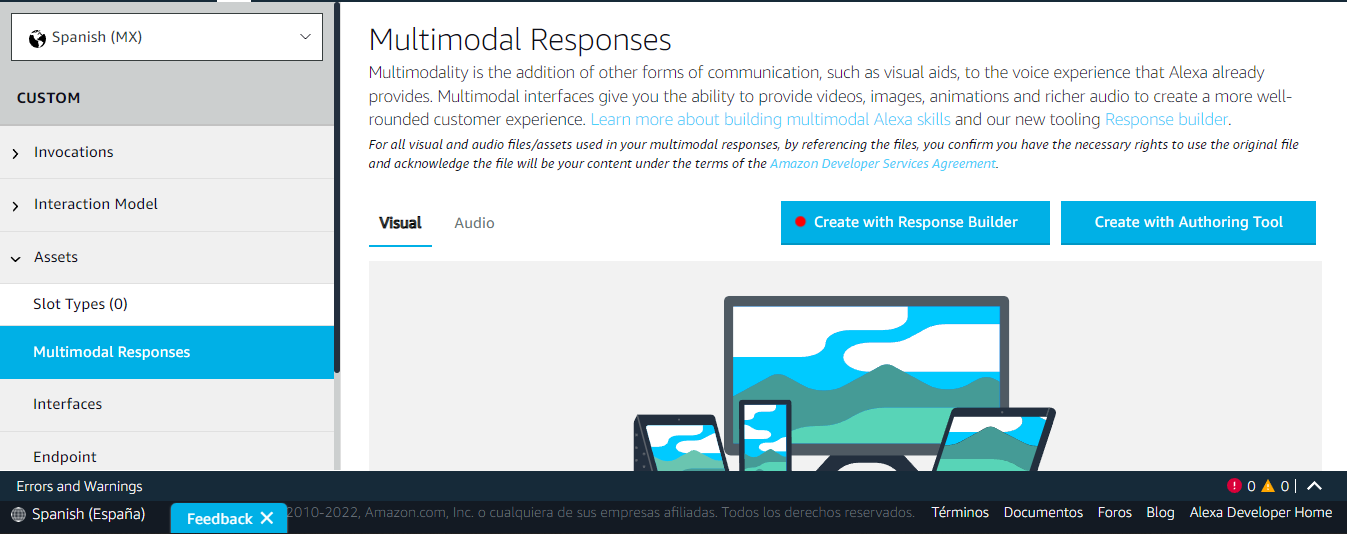
\includegraphics[width=0.70\textwidth]{Cap5/Figuras/AlexaMultimodalResponses.png}
  \caption{Interfaces con respuestas multimodales en la consola de desarrollo de Alexa.}
  \label{fig:51}
\end{figure}

La skill Buscador Gavilán, no es la excepción a la integración de interacción multimodal, en la que se pueden crear recursos visuales y táctiles. Es importante mencionar que la integración multimodal a una skill, está sujeta al diseño de una interfaz visual, por lo que sería necesario definir herramientas como el Customer Journey Map, un mapa de navegación, así como pruebas con usuarios para evaluar la usabilidad de la interfaz gráfica. Con el fin de limitar la skill Buscador Gavilán a una interacción basada únicamente en el reconocimiento por voz, la integración de interfaces multimodales se propone como trabajo a futuro para crear una mejor experiencia con la skill.

Algunos prototipos de la interacción multimodal con el Buscador Gavilán se presentan a continuación. Cabe destacar que estos sólo son prototipos de prueba para la integración multimodal, más no una versión final de los elementos visuales que presentan.

En la Figura \ref{fig:52} se muestra una propuesta para la bienvenida a la skill, una vez que es activado el LaunchRequestHandler a partir de uno de los comandos de activación de la skill.

\begin{figure}[H]
  \centering
  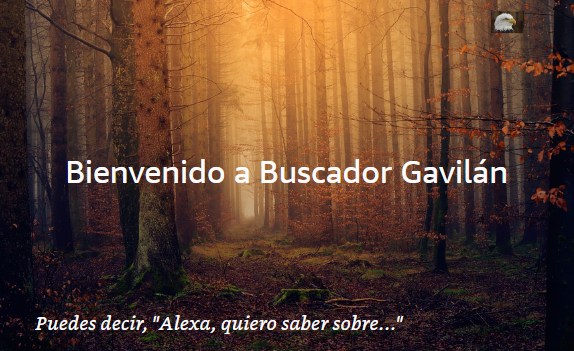
\includegraphics[width=0.60\textwidth]{Cap5/Figuras/Multimodal1.png}
  \caption{Respuesta multimodal de bienvenida al Buscador Gavilán.}
  \label{fig:52}
\end{figure}

En la Figura \ref{fig:53} se muestra una propuesta para el listado de preguntas sugeridas para elegir una pregunta inicial.

\begin{figure}[H]
  \centering
  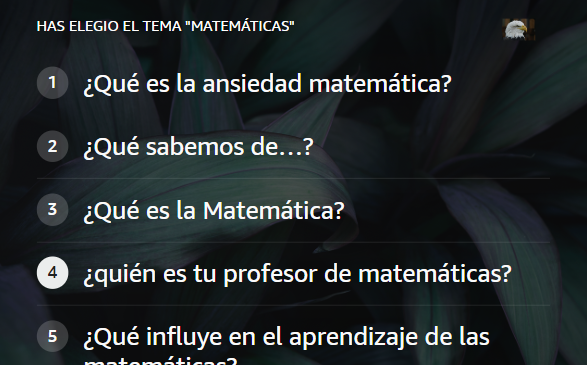
\includegraphics[width=0.60\textwidth]{Cap5/Figuras/Multimodal2.png}
  \caption{Respuesta multimodal para el listado de preguntas sugeridas del Buscador Gavilán.}
  \label{fig:53}
\end{figure}

En la Figura \ref{fig:54} se muestra una propuesta para el listado de fuentes de información con el dominio del cual se consulta la información.

\begin{figure}[H]
  \centering
  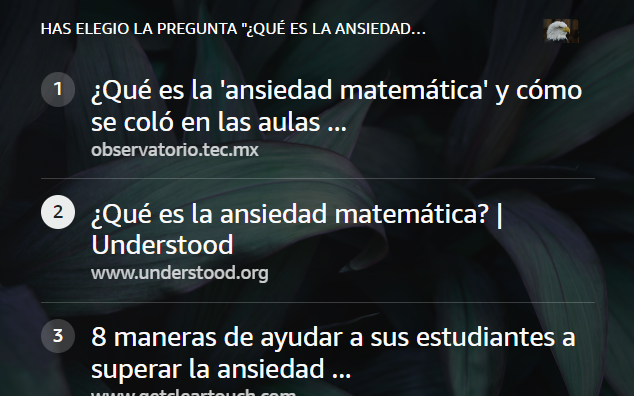
\includegraphics[width=0.60\textwidth]{Cap5/Figuras/Multimodal3.png}
  \caption{Respuesta multimodal para el listado de fuentes de información del Buscador Gavilán.}
  \label{fig:54}
\end{figure}

En la Figura \ref{fig:55} se muestra una propuesta para mostrar la información contenida en alguna de las fuentes de información elegida por el usuario.

\begin{figure}[H]
  \centering
  \includegraphics[width=0.60\textwidth]{Cap5/Figuras/Multimodal4.png}
  \caption{Respuesta multimodal para mostrar contenido de una fuente de información elegida.}
  \label{fig:55}
\end{figure}

En la Figura \ref{fig:56} se muestra una propuesta para mostrar al usuario las sugerencias generales para incorporar en la investigación final, así como brindarle la posibilidad de integrar un recordatorio.

\begin{figure}[H]
  \centering
  \includegraphics[width=0.60\textwidth]{Cap5/Figuras/Multimodal5.png}
  \caption{Respuesta multimodal para sugerir recomendaciones al usuario.}
  \label{fig:56}
\end{figure}

En la Figura \ref{fig:57} se muestra una propuesta para mostrar las recomendaciones para representar la información de la investigación final, así como la despedida de la skill.

\begin{figure}[H]
  \centering
  \includegraphics[width=0.60\textwidth]{Cap5/Figuras/Multimodal6.png}
  \caption{Respuesta multimodal para sugerir herramientas de representación de información.}
  \label{fig:57}
\end{figure}



%------------------------------------------------------------
%	APÉNDICES
%------------------------------------------------------------
	
\appendix

%------------------------------------------------------------
%	Anexo 1
%------------------------------------------------------------

\chapter{Código del Buscador Gavilán}
\label{Anexo1}

%------------------------------------------------------------
%	Web Scraper
%------------------------------------------------------------

\section{Web Scraper}
\label{A1Anexo}

\begin{tcolorbox}[colback=white!25!white,colframe=blue]
  \begin{minted}{python}
import requests
from bs4 import BeautifulSoup

class WebScraper:
  """
  Aplicador de Web Scraping para obtener el contenido de una 
  página web a partir de su URL.
  """

  def __init__(self, url):
    """
    Crea un nuevo web scraper
    Parámetro
    url -- url semilla de donde comenzar la búsqueda
    """
    self.url = url

    # Obtención del contenido de la url
    answer = requests.get(url)
    soup = BeautifulSoup(answer.text)

    # Lista de párrafos
    self.container_text = soup.find_all('p')

    # Contador de párrafo actual
    self.current = -1
    
  def has_next(self):
    """
    Verifica si quedan párrafos por leer.
    """
    return self.current+1 != len(self.container_text)
  \end{minted}
\end{tcolorbox}

\begin{tcolorbox}[colback=white!25!white,colframe=blue]
  \begin{minted}{python}
  def next(self):
    """
    Regresa el párrafo actual de lectura
    """
    self.current += 1
        
    while self.has_next() and len(self.container_text[self.current].text)<40:
      self.current += 1
        
    try:
      return self.container_text[self.current].text 
    except:
      return "Lo siento, no hay más párrafos por leer."
    
  def current_info(self):
    """
    Regresa el puntero al párrafo actual
    """
    if self.current != -1:
      return self.container_text[self.current].text
    else:
      return "Lo siento, no hay más párrafos por leer."
  \end{minted}
\end{tcolorbox}

Donde:

\begin{itemize}
  \item \textbf{Constructor.} La función que construye una nueva instancia de WebScraper, recibe como parámetro la url de la cuál se extraerán los datos. En el cuerpo de la función se crea una nueva instancia de BeautifulSoup y se obtienen todos los párrafos contenidos en el sitio.
  \item \textbf{has\_next.} Verifica si hay párrafos por recorrer en el sitio. Regresa \texttt{true} si existen párrafos y \texttt{false} en caso de haber recorrido todos los párrafos.
  \item \textbf{next.} Obtiene el párrafo seguido del párrafo actual en el recorrido.
  \item \textbf{current\_info.} Devuelve el párrafo actual del recorrido.
\end{itemize}

%------------------------------------------------------------
%	LaunchRequestHandler
%------------------------------------------------------------

\section{LaunchRequestHandler}
\label{A2Anexo}

\begin{tcolorbox}[colback=white!25!white,colframe=blue]
  \begin{minted}{python}
class LaunchRequestHandler(AbstractRequestHandler):
  """Handler for Skill Launch."""
  def can_handle(self, handler_input):
    # type: (HandlerInput) -> bool

    return ask_utils.is_request_type("LaunchRequest")(handler_input)

  def handle(self, handler_input):
    # type: (HandlerInput) -> Response
        
    speak_output = "Bienvenido al buscador gavilán. Te ayudaré a investigar"+ 
      "información de cualquier tema que desees. Puedes decir quiero saber sobre."+
      "Para comenzar con la investigación. ¿Sobre qué tema te gustaría investigar?"
    response_builder = handler_input.response_builder
        
    global help_id
    help_id = 0

    return response_builder.speak(speak_output).ask(speak_output).response
  \end{minted}
\end{tcolorbox}

%------------------------------------------------------------
%	CancelOrStopIntentHandler
%------------------------------------------------------------

\section{CancelOrStopIntentHandler}
\label{A3Anexo}

\begin{tcolorbox}[colback=white!25!white,colframe=blue]
  \begin{minted}{python}
class CancelOrStopIntentHandler(AbstractRequestHandler):
  """Single handler for Cancel and Stop Intent."""
  def can_handle(self, handler_input):
    # type: (HandlerInput) -> bool
    return (ask_utils.is_intent_name("AMAZON.CancelIntent")(handler_input) or
      ask_utils.is_intent_name("AMAZON.StopIntent")(handler_input))

  def handle(self, handler_input):
    # type: (HandlerInput) -> Response
    speak_output = "Gracias por investigar con la ayuda del buscador gavilán."+
      "Hasta pronto."

    return (
      handler_input.response_builder
        .speak(speak_output)
        .response
    )
  \end{minted}
\end{tcolorbox}

%------------------------------------------------------------
%	HelpIntentHandler
%------------------------------------------------------------

\section{HelpIntentHandler}
\label{A4Anexo}

\begin{tcolorbox}[colback=white!25!white,colframe=blue]
  \begin{minted}{python}
help_list = [
    "Puedes decir quiero saber sobre. Para comenzar una nueva investigación",
    "Puedes elegir una de las preguntas sugeridas o buscar otra pregunta "+
      "inicial diciendo sí o no",
    "Puedes elegir una de las referencias sugeridas o solicitar otra diciendo "+
      "sí o no",
    "Puedes solicitar guardar la referencia o pedir que diga el siguiente "+
      "párrafo si lo deseas",
    "Puedes solicitar más información del tema diciendo lee siguiente párrafo "+
      "o continúa con la investigación para consultar más referencias",
    "Puedes terminar la investigación o solicitar nuevas referencias",
    "Puedes decir agrega recordatorio u omitir recordatorio. Ya casi terminamos "+
      "la investigación",
    "Puedes decir cierra la skill para salir o preguntar sobre un nuevo tema"
]

class HelpIntentHandler(AbstractRequestHandler):
  """Handler for Help Intent."""
  def can_handle(self, handler_input):
    # type: (HandlerInput) -> bool
    return ask_utils.is_intent_name("AMAZON.HelpIntent")(handler_input)

  def handle(self, handler_input):
    # type: (HandlerInput) -> Response
    speak_output = help_list[help_id] + ". " + last_request

    return (
      handler_input.response_builder
        .speak(speak_output)
        .ask(speak_output)
        .response
      )
  \end{minted}
\end{tcolorbox}

%------------------------------------------------------------
%	FallbackIntentHandler
%------------------------------------------------------------

\section{FallbackIntentHandler}
\label{A5Anexo}

\begin{tcolorbox}[colback=white!25!white,colframe=blue]
  \begin{minted}{python}
class FallbackIntentHandler(AbstractRequestHandler):
  """Single handler for Fallback Intent."""
  def can_handle(self, handler_input):
    # type: (HandlerInput) -> bool
    return ask_utils.is_intent_name("AMAZON.FallbackIntent")(handler_input)

  def handle(self, handler_input):
    # type: (HandlerInput) -> Response
    logger.info("In FallbackIntentHandler")
    speech = "No entendí tu petición. Puedes decir ayuda para solicitar más "+
      "información. " + last_request
    reprompt = "No entendí tu petición. Puedes decir solicitar ayuda en "+
      "cualquier momento para apoyarte. " + last_request

    return handler_input.response_builder.speak(speech).ask(reprompt).response
  \end{minted}
\end{tcolorbox}

%------------------------------------------------------------
%	tellTopicIntentHandler
%------------------------------------------------------------

\section{tellTopicIntentHandler}
\label{A6Anexo}

\begin{tcolorbox}[colback=white!25!white,colframe=blue]
  \begin{minted}{python}
class tellTopicIntentHandler(AbstractRequestHandler):
  def can_handle(self, handler_input):
    # type: (HandlerInput) -> bool
    return ask_utils.is_intent_name("tellTopicIntent")(handler_input)

  def handle(self, handler_input):
        
    global questions
    global question
    global isQuestion
    global searcherContent
    global reference
    global mainTopic
    global list_info
    global last_request
    global list_titles
    global help_id
        
    questions = None
    help_id = 1
    question = 0
    isQuestion = True
    searcherContent = None
    reference = 0
    list_info = []
    last_request = ""
    list_titles = []
  \end{minted}
\end{tcolorbox}

\begin{tcolorbox}[colback=white!25!white,colframe=blue]
  \begin{minted}{python}    
    slotsFromIntent = handler_input.request_envelope.request.intent.slots
    topic = slotsFromIntent['searchWord']
    mainTopic = topic
    
    s = srch.Searcher(str(topic.value), True)
    
    questions = s.listQuestions()

    indice = random.randint(0, len(pregunta_inicial) - 1)
    speak_output = "Una pregunta inicial te ayudará a profundizar el tema que "+
      "deseas investigar, te presentaré algunas sugerencias para apoyarte." + 
      questions[question] + ". " + pregunta_inicial[indice]
    last_request = speak_output
    isQuestion = True

    return (
      handler_input.response_builder
        .speak(speak_output)
        .ask(speak_output)
        .response
      )
  \end{minted}
\end{tcolorbox}

%------------------------------------------------------------
%	yesAmazonIntentHandler
%------------------------------------------------------------

\section{yesAmazonIntentHandler}
\label{A7Anexo}

\begin{tcolorbox}[colback=white!25!white,colframe=blue]
  \begin{minted}{python}
class yesAmazonIntentHandler(AbstractRequestHandler):
  """Handler for Hello World Intent."""
  def can_handle(self, handler_input):
    # type: (HandlerInput) -> bool
    return ask_utils.is_intent_name("AMAZON.YesIntent")(handler_input)

  def handle(self, handler_input):
    # type: (HandlerInput) -> Response
    
    global searcherContent
    speak_output = ""
    global isQuestion
    global scraper
    global mainTopic
    global last_request
    global help_id
    
    last_request = ""
    
    if questions==None:
        speak_output = "Lo siento. Aún no tengo una pregunta inicial para iniciar"+
          " la investigación"
  \end{minted}
\end{tcolorbox}

\begin{tcolorbox}[colback=white!25!white,colframe=blue]
  \begin{minted}{python}   
    elif isQuestion:
      speak_output = "Has elegido la pregunta: " + questions[question]
      searcherContent = srch.Searcher(questions[question], False)
      searcherContent.lookForReferences()
      
      indice = random.randint(0, len(sugerencia_referencia)-1)
      speak_output += ". Encontré " + searcherContent.references[reference]['title']+ 
        " en " + searcherContent.references[reference]['displayLink'] + ". "
        +sugerencia_referencia[indice]
      help_id = 2
      isQuestion = False
    else:
      scraper = ws.WebScraper(searcherContent.references[reference]['link'],
        mainTopic)
      if scraper.has_next():
          nextInfo = str(scraper.next())
          speak_output = "Según " +
            searcherContent.references[reference]['displayLink']+
            " " + nextInfo + ", puedes decir 'guardar la referencia' para almacenar"+
            " o 'siguiente párrafo' para escuchar más de esta referencia o "+
            "'continuar con la investigación' para ir al siguiente paso"
          help_id = 3
          
      else:
          speak_output = "Lo siento, no pude acceder a la información de la"+
            " referencia. Aún así puedes almacenarla diciendo... guarda la "+
            "referencia"
  
    last_request = speak_output
        
    return (
      handler_input.response_builder
        .speak(speak_output)
        .ask(speak_output)
        .response
    )
  \end{minted}
\end{tcolorbox}

%------------------------------------------------------------
%	noAmazonIntentHandler
%------------------------------------------------------------

\section{noAmazonIntentHandler}
\label{A8Anexo}

\begin{tcolorbox}[colback=white!25!white,colframe=blue]
  \begin{minted}{python}
class noAmazonIntentHandler(AbstractRequestHandler):
  """Handler for Hello World Intent."""
  def can_handle(self, handler_input):
    # type: (HandlerInput) -> bool
    return ask_utils.is_intent_name("AMAZON.NoIntent")(handler_input)

  def handle(self, handler_input):
    # type: (HandlerInput) -> Response
    global question
    global questions
    global reference
    global last_request
    global help_id
    
    last_request = ""
        
    speak_output = ""
    if questions==None:
      speak_output = "Lo siento. Aún no tengo una pregunta inicial para iniciar la"+
      " investigación"
    elif isQuestion:
      question = (question + 1) % len(questions)
      speak_output = questions[question] + ". ¿Es tu pregunta inicial o busco otra "+
        "opción?"
      help_id = 1
    else:
      reference = (reference + 1) % len(searcherContent.references)
      speak_output = "Encontré " + searcherContent.references[reference]['title'] +
        " en " + searcherContent.references[reference]['displayLink'] + 
        ". ¿Consulto esta referencia o busco otra?"
      help_id = 2
    
    last_request = speak_output
    
    return (
      handler_input.response_builder
        .speak(speak_output)
        .ask(speak_output)
        .response
    )
  \end{minted}
\end{tcolorbox}

%------------------------------------------------------------
%	nextInfoIntentHandler
%------------------------------------------------------------

\section{nextInfoIntentHandler}
\label{A9Anexo}

\begin{tcolorbox}[colback=white!25!white,colframe=blue]
  \begin{minted}{python}
class nextInfoIntentHandler(AbstractRequestHandler):
  def can_handle(self, handler_input):
    # type: (HandlerInput) -> bool
    return ask_utils.is_intent_name("nextInfoIntent")(handler_input)

  def handle(self, handler_input):
        
    global scraper
    global last_request
    global help_id
        
    last_request = ""
    speak_output = ""
        
    if scraper == None:
      speak_output = "Lo siento, aún no has elegido tema o referencia"
    elif scraper.has_next():
      nextInfo = str(scraper.next())
      speak_output = nextInfo + ", puedes decir 'guardar la referencia' para "+
        "almacenar o 'siguiente párrafo' para escuchar más de esta referencia o "+
        "'continuar con la investigación' para ir al siguiente paso"
      help_id = 3
    else:
      nextInfoIntent = "Lo siento, ya no hay más información para mostrar en esta"+
        " referencia. Puedes almacenarla diciendo... Guarda la referencia"
      help_id = 3
    
    last_request = speak_output
    return (
      handler_input.response_builder
        .speak(speak_output)
        .ask(speak_output)
        .response
    )
  \end{minted}
\end{tcolorbox}

%------------------------------------------------------------
%	continueIntentHandler
%------------------------------------------------------------

\section{continueIntentHandler}
\label{A10Anexo}

\begin{tcolorbox}[colback=white!25!white,colframe=blue]
  \begin{minted}{python}
class continueIntentHandler(AbstractRequestHandler):
  def can_handle(self, handler_input):
    # type: (HandlerInput) -> bool
    return ask_utils.is_intent_name("continueIntent")(handler_input)

  def handle(self, handler_input):
        
    global last_request
    global help_id
        
    last_request = ""
        
    speak_output = "Puedes decir 'consultar más fuentes' para investigar más o"+
      " 'terminar la investigación' para continuar"
    help_id = 5
    last_request = speak_output
        
    return (
      handler_input.response_builder
        .speak(speak_output)
        .ask(speak_output)
        .response
    )
  \end{minted}
\end{tcolorbox}

%------------------------------------------------------------
%	endInvestigationIntentHandler
%------------------------------------------------------------

\section{endInvestigationIntentHandler}
\label{A11Anexo}

\begin{tcolorbox}[colback=white!25!white,colframe=blue]
  \begin{minted}{python}
class endInvestigationIntentHandler(AbstractRequestHandler):
  def can_handle(self, handler_input):
    # type: (HandlerInput) -> bool
    return ask_utils.is_intent_name("endInvestigationIntent")(handler_input)

  def handle(self, handler_input):
        
    global last_request
    global help_id
        
    help_id = 6
    last_request = ""
    speak_output = "No olvides agregar tu nombre y fuentes consultadas en la "+
      "investigación. Puedes decir 'agrega recordatorio' para no olvidar la fecha "+
      "de entrega. También puedes saltar el recordatorio diciendo 'omitir "+
      "recordatorio'"
    last_request = speak_output
  \end{minted}
\end{tcolorbox}

\begin{tcolorbox}[colback=white!25!white,colframe=blue]
  \begin{minted}{python}            
    return (
      handler_input.response_builder
        .speak(speak_output)
        .ask(speak_output)
        .response
    )
  \end{minted}
\end{tcolorbox}

%------------------------------------------------------------
%	addReminderIntentHandler
%------------------------------------------------------------

\section{addReminderIntentHandler}
\label{A12Anexo}

\begin{tcolorbox}[colback=white!25!white,colframe=blue]
  \begin{minted}{python}
class addReminderIntentHandler(AbstractRequestHandler):
  def can_handle(self, handler_input):
    # type: (HandlerInput) -> bool
    return ask_utils.is_intent_name("addReminderIntent")(handler_input)

  def handle(self, handler_input):
        
    global last_request
    global help_id
        
    last_request =""
    help_id = 7
        
    slotsFromIntent = handler_input.request_envelope.request.intent.slots
        
    date = slotsFromIntent['date'].value
    speak_output = "Tu recordatorio está listo para " + date
        
    request_envelope = handler_input.request_envelope
    response_builder = handler_input.response_builder
    reminder_service = handler_input.service_client_factory.
      get_reminder_management_service()
        
    # Permisos para recordatorios
    if not (request_envelope.context.system.user.permissions and
      request_envelope.context.system.user.permissions.consent_token):
            
      return response_builder.add_directive(
        SendRequestDirective(
          name="AskFor",
          payload={
            "@type": "AskForPermissionsConsentRequest",
            "@version": "1",
            "permissionScope": "alexa::alerts:reminders:skill:readwrite"
          },
          token="correlationToken"
        )
      ).response
  \end{minted}
\end{tcolorbox}

\begin{tcolorbox}[colback=white!25!white,colframe=blue]
  \begin{minted}{python}
    # Creación de recordatorio
    date_components = str(date).split("-")
    notification_time = date_components[0]+"-"+date_components[1]+"-"+
      date_components[2]+"T23:59:00"

    trigger = Trigger(object_type = TriggerType.SCHEDULED_ABSOLUTE, 
      scheduled_time = notification_time)
    text = SpokenText(locale='es-es', ssml = "<speak>Este es un recordatorio del "+
      "buscador Gavilán. No olvides entregar tu Investigación sobre" + 
      str(mainTopic.value) +"</speak>", text= 'Investigación de ' + 
      str(mainTopic.value) + ". No olvides "+"entregar tu Investigación.")
    alert_info = AlertInfo(AlertInfoSpokenInfo([text]))
    push_notification = PushNotification(PushNotificationStatus.ENABLED)
    reminder_request = ReminderRequest(notification_time , trigger, alert_info, 
      push_notification)

    try:
      reminder_response = reminder_service.create_reminder(reminder_request)
      logger.info("Reminder Created: {}".format(reminder_response))
    except ServiceException as e:
      logger.info("Exception encountered: {}".format(e.body))
      return response_builder.
        speak('Lo siento. No se pudo crear el recordatorio').response
        
    # Envío de datos al celular
    card_title = "Buscador Gavilán"
    card_text = ""
        
    if len(list_info) != 0:
      speak_output += ". Las referencias finales de la investigación son "
          
      for data in list_titles:
        speak_output += data + ". "
          
      message = ""
      for data in list_info:
        message += f"* {data}\n"
            
      speak_output += "Puedes consultar estas referencias en la app de Alexa. "
      #card_title = "Buscador Gavilán"
      card_text = message
  \end{minted}
\end{tcolorbox}

\begin{tcolorbox}[colback=white!25!white,colframe=blue]
  \begin{minted}{python} 
    remember_message = " Recuerda que puedes presentar la información en una "+
      "gráfica, un cuadro comparativo, una tabla, un artículo, un cuadro "+
      "sinóptico, un reporte o incluso en un dibujo. Gracias por investigar con"+
      " la ayuda del buscador gavilán, hasta pronto."
    speak_output += remember_message
        
    last_request = speak_output
        
    return (
      handler_input.response_builder
        .speak(speak_output)
        #.ask(speak_output) # Aquí termina la skill
        .response
    )
  \end{minted}
\end{tcolorbox}

%------------------------------------------------------------
%	omitIntentHandler
%------------------------------------------------------------

\section{omitIntentHandler}
\label{A13Anexo}

\begin{tcolorbox}[colback=white!25!white,colframe=blue]
  \begin{minted}{python}
class omitIntentHandler(AbstractRequestHandler):
  def can_handle(self, handler_input):
    # type: (HandlerInput) -> bool
    return ask_utils.is_intent_name("omitIntent")(handler_input)

  def handle(self, handler_input):
        
    global last_request
    global help_id
        
    help_id = 7
    last_request = ""
    speak_output = ""
        
    card_title = "Buscador Gavilán"
    card_text = ""
        
    if len(list_info) != 0:
      speak_output += "Las referencias finales de la investigación son las "+
        "siguientes. "
            
      for data in list_titles:
        speak_output += data + ". "
            
      message = ""
      for data in list_info:
        message += f"* {data}\n"
  \end{minted}
\end{tcolorbox}

\begin{tcolorbox}[colback=white!25!white,colframe=blue]
  \begin{minted}{python}
      speak_output += "Puedes consultar estas referencias en la app de Alexa."
      #card_title = "Buscador Gavilán"
      card_text = message
      
    remember_message = "Recuerda que puedes presentar la información en una "+
      "gráfica, un cuadro comparativo, una tabla, un artículo, un cuadro "+
      "sinóptico, un reporte o incluso en un dibujo. Gracias por investigar con "+
      "la ayuda del buscador gavilán, hasta pronto."
    speak_output += remember_message
         
    last_request = speak_output
        
    if len(list_info) != 0:
      return (
        handler_input.response_builder
          .speak(speak_output)
          .set_card(SimpleCard(card_title, card_text))
          #.ask(speak_output) # Aqui se termina la skill
          .response
      )
    else:
      return (
        handler_input.response_builder
          .speak(speak_output)
          #.ask(speak_output) # Aqui se termina la skill
          .response
      )
  \end{minted}
\end{tcolorbox}

%------------------------------------------------------------
%	lastRequestIntentHandler
%------------------------------------------------------------

\section{lastRequestIntentHandler}
\label{A14Anexo}

\begin{tcolorbox}[colback=white!25!white,colframe=blue]
  \begin{minted}{python}
class lastRequestIntentHandler(AbstractRequestHandler):
  def can_handle(self, handler_input):
    # type: (HandlerInput) -> bool
    return ask_utils.is_intent_name("lastRequestIntent")(handler_input)

  def handle(self, handler_input):
        
    global last_request
        
    speak_output = last_request
                
    return (
      handler_input.response_builder
        .speak(speak_output)
        .ask(speak_output)
        .response
    )

  \end{minted}
\end{tcolorbox}

%------------------------------------------------------------
%	Anexo 2
%------------------------------------------------------------

\chapter{Evaluación de la skill}
\label{Anexo2}

%------------------------------------------------------------
%	Cuestionario de entrada
%------------------------------------------------------------

\section{Cuestionario de entrada}
\label{B1Anexo}

\begin{tcolorbox}[colback=white!25!white,colframe=blue]
  \begin{enumerate}
    \item Edad
    \item Sexo
    \item ¿Qué semestre estás cursando?
    \item ¿Con qué frecuencia investigas en las siguientes fuentes? (Nunca, Casi nunca, Frecuentemente, Muy frecuentemente)
    \item ¿Qué dispositivos utilizas para realizar una investigación en Internet?
    \item Por lo general, ¿buscas temas de interés personal o con propósito académico en Internet?
    \item Al recuperar información (imagen, texto, video) ¿incluyes las referencias consultadas?
    \item Justifica tu respuesta anterior
    \item ¿Cómo consideras que es la información que obtienes al final de una investigación?
    \item De las siguientes fuentes de información, ¿cuáles sueles consultar?
    \item ¿Utilizas algún método de investigación?
    \item Si tu respuesta anterior fue afirmativa, ¿cuáles métodos de investigación has usado?
    \item ¿Conoces el Modelo Gavilán?
    \item Si tu respuesta anterior fue afirmativa, ¿alguna vez has llevado a la práctica el proceso de investigación con el Modelo Gavilán?
    \item ¿Cuánto tiempo te toma investigar un tema?
    \item ¿Sabes qué es un asistente basado en voz?
    \item Si tu respuesta anterior fue afirmativa, ¿cuál o cuáles asistentes basados en voz conoces?
    \item ¿Alguna vez has utilizado un asistente basado en voz?
    \item Si tu respuesta anterior fue afirmativa, ¿con qué fin sueles usar un asistente basado en voz?
    \item ¿Sabes qué es una skill para el asistente basado en voz de Amazon?
    \item Si has usado un asistente basado en voz. ¿Qué tan cómodo te sientes usándolo?
    \item ¿Crees que investigar con apoyo de un asistente basado en voz podría ayudar en el proceso de investigación?
    \item Justifica tu respuesta
  \end{enumerate}
\end{tcolorbox}

%------------------------------------------------------------
%	Protocolo de bienvenida
%------------------------------------------------------------

\section{Protocolo de bienvenida}
\label{B2Anexo}

\begin{tcolorbox}[colback=white!25!white,colframe=blue]
  Fecha de la prueba: \_\_\_\_ de \_\_\_\_\_\_\_\_\_\_\_\_\_\_\_ de 2021

  Buenos días/tardes, gracias por brindarnos unos minutos de su tiempo. Mi nombre es \_\_\_\_\_\_\_\_\_\_ y estaré contigo en esta sesión.

  Permíteme profundizar sobre la razón del porqué nos encontramos aquí.

  Estamos probando una skill que será un apoyo al proceso de investigación por medio del reconocimiento por voz. Antes de continuar, quiero comentarte que las skills son funcionalidades que permiten a los usuarios del asistente de voz Alexa de Amazon, crear una experiencia más personalizada.

  Esta sesión será grabada, ya que mediante el estudio de tus comentarios, podremos identificar las posibles mejoras de la skill, por lo que te pedimos que actúes con naturalidad. También te pedimos que expreses tus opiniones en voz alta, ya que este ejercicio tiene el propósito de evaluar a la skill y no a ti.

  Dado que es una skill que está en proceso de desarrollo, se podrían presentar situaciones imprevistas, así que te agradecemos considerarlo.

  Se presentará un prototipo y se te pedirá que realices algunas tareas típicas para las cuales está diseñada la skill. La sesión consistirá en que efectúes dichas tareas y describas en voz alta tus acciones, así como cualquier opinión que tengas, ya que serán de gran utilidad para mejorar la skill.

  Cuando comience la sesión, te puedes sentir en total libertad de hacer cualquier pregunta, aunque no podré contestar algunas de ellas, ya que el objetivo es simular una situación real en la que la skill opere de manera autónoma.
  Veamos un video sobre el funcionamiento de Alexa.

  Interactuarás con la Alexa que está con Emmanuel. Tu tarea será utilizar la skill llamada Buscador Gavilán, para investigar sobre un tema y realizar otras actividades que se permiten y se presentan a continuación.

  \begin{itemize}
    \item La skill se llama Buscador Gavilán
    \item Te permite investigar sobre un tema, para la prueba investigarás sobre matemáticas
    \item Te sugiere diferentes preguntas iniciales
    \item Te recomienda diferentes referencias
    \item Te da más información del tema
    \item Almacena la referencia de la información
    \item Puedes programar un recordatorio. Al final debes programar un recordatorio para el 10 diciembre.
  \end{itemize}

  Interactúa libremente con la skill, te pedimos que trates de probar todas las funciones. Puedes terminar cuando tú quieras.

  ¿Tienes alguna duda?
  Puedes comenzar a usar la skill.

\end{tcolorbox}

%------------------------------------------------------------
%	Actividades de la prueba
%------------------------------------------------------------

\section{Actividades de la prueba}
\label{B3Anexo}

\begin{tcolorbox}[colback=white!25!white,colframe=blue]
  Usuario No: \_\_\_\_\_\_\_\_\_\_\_\_\_\_\_\_\_\_\_\_\_\_\_\_\_\_\_\_\_\_\_\_\_\_\_\_\_\_\_\_\_\_\_\_\_\_\_\_\_\_\_\_\_\_
  Fecha de evaluación: \_\_\_\_\_\_\_\_\_ de \_\_\_\_\_\_\_\_\_\_\_\_\_\_\_\_\_\_\_\_\_\_\_ de 2021
  Hora de inicio: \_\_\_\_\_\_\_\_\_\_\_\_\_\_\_\_\_\_\_\_\_\_\_\_\_\_\_\_\_\_\_\_\_\_\_\_\_\_\_\_\_\_\_\_\_\_\_\_\_\_

  \textbf{Instrucciones para el moderador}
  \begin{enumerate}
    \item Ir tachando las actividades realizadas con el fin de no perderse durante la prueba. NO se realizará ninguna actividad si antes no ha concluido la anterior (a menos que se le instruya lo contrario).
    \item En caso de que el usuario cometa algún error preguntar:
    \textit{¿La skill le informó con claridad qué fue lo que pasó?}
  \end{enumerate}

  \begin{itemize}
    \item Activa la skill
    Nota para el monitor: Decir la frase “Alexa, abre buscador gavilán”
    \item Solicita a la skill investigar sobre el tema de matemáticas
    Nota para el monitor: Decir la frase “Alexa, quiero saber sobre matemáticas”
    \item Solicita a Alexa que te sugiera una nueva pregunta inicial
    Nota para el monitor: Decir la frase “Alexa, busca otra opción”
    \item Solicita a Alexa que utilice la pregunta inicial sugerida
    Nota para el monitor: Decir la siguiente frase “Alexa, sí es mi pregunta inicial”
    \item Solicita a Alexa que te recomiende otra referencia
    Nota para el monitor: Decir la siguiente frase “Alexa, consulta más fuentes”
    \item Solicita a Alexa que utilice la referencia propuesta
    Nota para el monitor: Decir la frase “Alexa, quiero esa referencia”
    \item Solicita a la skill más información del tema
    Nota para el monitor: Decir la frase “Alexa, lee siguiente párrafo”
    \item Solicita a la skill buscar otra referencia
    Nota para el monitor: Decir la frase ”Alexa, seguir investigando”
    \item Solicita a Alexa que almacene la referencia de la información
    Nota para el monitor: Decir la frase “Alexa, guarda la referencia”
    \item Solicita a Alexa que continúe con la investigación
    Nota para el monitor: Decir la frase “Alexa, continúa con la investigación”
    \item Solicita a Alexa finalizar con la investigación
    Nota para el monitor: Decir la frase “Alexa, termina la investigación”
    \item Solicita a la skill que programe un recordatorio para el 10 diciembre
    Nota para el monitor: Decir la frase “Alexa, agrega recordatorio para el 10 de diciembre”
    \item Solicita a Alexa salir de la skill
    Nota para el monitor: Decir la frase “Alexa, cierra la skill”
  \end{itemize}

  Gracias por participar en la evaluación.

  Anotar hora en que terminó la evaluación \_\_\_\_\_\_\_\_\_\_\_\_\_\_\_\_\_\_\_\_\_\_\_\_\_\_\_\_\_\_\_\_\_\_\_
  
  Notas del moderador:

  \_\_\_\_\_\_\_\_\_\_\_\_\_\_\_\_\_\_\_\_\_\_\_\_\_\_\_\_\_\_\_\_\_\_\_\_\_\_\_\_\_\_\_\_\_\_\_\_\_\_\_\_\_\_\_\_

  \_\_\_\_\_\_\_\_\_\_\_\_\_\_\_\_\_\_\_\_\_\_\_\_\_\_\_\_\_\_\_\_\_\_\_\_\_\_\_\_\_\_\_\_\_\_\_\_\_\_\_\_\_\_\_\_

  \_\_\_\_\_\_\_\_\_\_\_\_\_\_\_\_\_\_\_\_\_\_\_\_\_\_\_\_\_\_\_\_\_\_\_\_\_\_\_\_\_\_\_\_\_\_\_\_\_\_\_\_\_\_\_\_

  \_\_\_\_\_\_\_\_\_\_\_\_\_\_\_\_\_\_\_\_\_\_\_\_\_\_\_\_\_\_\_\_\_\_\_\_\_\_\_\_\_\_\_\_\_\_\_\_\_\_\_\_\_\_\_\_

  \_\_\_\_\_\_\_\_\_\_\_\_\_\_\_\_\_\_\_\_\_\_\_\_\_\_\_\_\_\_\_\_\_\_\_\_\_\_\_\_\_\_\_\_\_\_\_\_\_\_\_\_\_\_\_\_

  \_\_\_\_\_\_\_\_\_\_\_\_\_\_\_\_\_\_\_\_\_\_\_\_\_\_\_\_\_\_\_\_\_\_\_\_\_\_\_\_\_\_\_\_\_\_\_\_\_\_\_\_\_\_\_\_

\end{tcolorbox}

%------------------------------------------------------------
%	Guión de actividades para la evaluación
%------------------------------------------------------------

\section{Guión de actividades para la evaluación}
\label{B4Anexo}

\begin{tcolorbox}[colback=white!25!white,colframe=blue]
  \textbf{Funciones}
  \begin{itemize}
    \item La skill se llama Buscador Gavilán
    \item Te permite investigar sobre un tema, para la prueba investigarás sobre matemáticas
    \item Te sugiere diferentes preguntas iniciales
    \item Te recomienda diferentes referencias
    \item Te da más información del tema
    \item Almacena la referencia de la información
    \item Puedes programar un recordatorio, al final debes programar un recordatorio para el 10 diciembre
  \end{itemize}

  Interactúa libremente con la skill, te pedimos que trates de probar todas las funciones.
  Puedes terminar cuando tú quieras.

\end{tcolorbox}

%------------------------------------------------------------
%	Cuestionario de usabilidad
%------------------------------------------------------------

\section{Cuestionario de usabilidad}
\label{B5Anexo}

\begin{tcolorbox}[colback=white!25!white,colframe=blue]
  Lea cuidadosamente las siguientes afirmaciones y marque con una x que tan de acuerdo o desacuerdo está con ellas, considerando que 5 es equivalente a fuertemente desacuerdo y 1 a fuertemente de acuerdo. Si no está seguro (a) de que contestar marque 3.

  \begin{tabular}{| p{4cm} | p{2cm} | p{2cm} | p{2cm} | p{2cm} | p{2cm} |}
    \hline
     & \multicolumn{1}{p{2cm}}{Fuertemente en desacuerdo}  & \multicolumn{3}{p{2cm}}{} & Fuertemente de acuerdo \\ \hline
     & 5 & 4 & 3 & 2 & 1 \\ \hline
    Creo que me gustaría usar la skill frecuentemente. &  &  &  &  &  \\ \hline
    Encuentro la skill compleja. &  &  &  &  &  \\ \hline
    Pienso que la skill es fácil de usar. &  &  &  &  &  \\ \hline
    Creo que necesitaré la ayuda de un técnico para usar la skill. &  &  &  &  &  \\ \hline
    Encontré que las distintas funciones de la skill estaban bien integrados. &  &  &  &  &  \\ \hline
    Pienso que había mucha inconsistencia en la skill. &  &  &  &  &  \\ \hline
    Me imagino que la gente aprenderá a usar la skill bastante rápido. &  &  &  &  &  \\ \hline
    Encuentro la skill engorrosa de usar. &  &  &  &  &  \\ \hline
    Me sentí muy seguro usando la skill. &  &  &  &  &  \\ \hline
    Necesito aprender muchas cosas antes de poder utilizar la skill. &  &  &  &  &  \\ \hline
  \end{tabular}

\end{tcolorbox}

%------------------------------------------------------------
%	Cuestionario de percepción subjetiva
%------------------------------------------------------------

\section{Cuestionario de percepción subjetiva}
\label{B6Anexo}

\begin{tcolorbox}[colback=white!25!white,colframe=blue]
  \textbf{Reacciones globales de la skill}

  \begin{tabular}{| p{1cm} | p{1cm} | p{1cm} | p{1cm} | p{1cm} | p{1cm} | p{1cm} | p{1cm} | p{1cm} | p{1cm} |}
    \multicolumn{2}{p{1cm}}{Terrible} & \multicolumn{6}{p{1cm}}{} & \multicolumn{2}{p{1cm}}{Maravilloso} \\ \hline
    1 & 2 & 3 & 4 & 5 & 6 & 7 & 8 & 9 & NA \\ \hline
  \end{tabular}

  \begin{tabular}{| p{1cm} | p{1cm} | p{1cm} | p{1cm} | p{1cm} | p{1cm} | p{1cm} | p{1cm} | p{1cm} | p{1cm} |}
    \multicolumn{2}{p{1cm}}{Frustrante} & \multicolumn{6}{p{1cm}}{} & \multicolumn{2}{p{1cm}}{Satisfactoria} \\ \hline
    1 & 2 & 3 & 4 & 5 & 6 & 7 & 8 & 9 & NA \\ \hline
  \end{tabular}

  \begin{tabular}{| p{1cm} | p{1cm} | p{1cm} | p{1cm} | p{1cm} | p{1cm} | p{1cm} | p{1cm} | p{1cm} | p{1cm} |}
    \multicolumn{2}{p{1cm}}{Aburrida} & \multicolumn{6}{p{1cm}}{} & \multicolumn{2}{p{1cm}}{Estimulante} \\ \hline
    1 & 2 & 3 & 4 & 5 & 6 & 7 & 8 & 9 & NA \\ \hline
  \end{tabular}

  \begin{tabular}{| p{1cm} | p{1cm} | p{1cm} | p{1cm} | p{1cm} | p{1cm} | p{1cm} | p{1cm} | p{1cm} | p{1cm} |}
    \multicolumn{2}{p{1cm}}{Difícil} & \multicolumn{6}{p{1cm}}{} & \multicolumn{2}{p{1cm}}{Fácil} \\ \hline
    1 & 2 & 3 & 4 & 5 & 6 & 7 & 8 & 9 & NA \\ \hline
  \end{tabular}

  \begin{tabular}{| p{1cm} | p{1cm} | p{1cm} | p{1cm} | p{1cm} | p{1cm} | p{1cm} | p{1cm} | p{1cm} | p{1cm} |}
    \multicolumn{3}{p{2cm}}{Rígida} & \multicolumn{5}{p{1cm}}{} & \multicolumn{2}{p{1cm}}{Flexible} \\ \hline
    1 & 2 & 3 & 4 & 5 & 6 & 7 & 8 & 9 & NA \\ \hline
  \end{tabular}

  \hfill

  \textbf{Aprendizaje}

  Aprender a usar la skill

  \begin{tabular}{| p{1cm} | p{1cm} | p{1cm} | p{1cm} | p{1cm} | p{1cm} | p{1cm} | p{1cm} | p{1cm} | p{1cm} |}
    \multicolumn{2}{p{1cm}}{Difícil} & \multicolumn{6}{p{1cm}}{} & \multicolumn{2}{p{1cm}}{Fácil} \\ \hline
    1 & 2 & 3 & 4 & 5 & 6 & 7 & 8 & 9 & NA \\ \hline
  \end{tabular}

  Tiempo para aprender a usar la skill

  \begin{tabular}{| p{1cm} | p{1cm} | p{1cm} | p{1cm} | p{1cm} | p{1cm} | p{1cm} | p{1cm} | p{1cm} | p{1cm} |}
    \multicolumn{2}{p{1cm}}{Difícil} & \multicolumn{6}{p{1cm}}{} & \multicolumn{2}{p{1cm}}{Fácil} \\ \hline
    1 & 2 & 3 & 4 & 5 & 6 & 7 & 8 & 9 & NA \\ \hline
  \end{tabular}

  Recordar nombres y funcionalidades

  \begin{tabular}{| p{1cm} | p{1cm} | p{1cm} | p{1cm} | p{1cm} | p{1cm} | p{1cm} | p{1cm} | p{1cm} | p{1cm} |}
    \multicolumn{2}{p{1cm}}{Difícil} & \multicolumn{6}{p{1cm}}{} & \multicolumn{2}{p{1cm}}{Fácil} \\ \hline
    1 & 2 & 3 & 4 & 5 & 6 & 7 & 8 & 9 & NA \\ \hline
  \end{tabular}

  Las tareas se pueden realizar de manera directa

  \begin{tabular}{| p{1cm} | p{1cm} | p{1cm} | p{1cm} | p{1cm} | p{1cm} | p{1cm} | p{1cm} | p{1cm} | p{1cm} |}
    \multicolumn{2}{p{1cm}}{Difícil} & \multicolumn{6}{p{1cm}}{} & \multicolumn{2}{p{1cm}}{Fácil} \\ \hline
    1 & 2 & 3 & 4 & 5 & 6 & 7 & 8 & 9 & NA \\ \hline
  \end{tabular}

  Número de pasos por tarea

  \begin{tabular}{| p{1cm} | p{1cm} | p{1cm} | p{1cm} | p{1cm} | p{1cm} | p{1cm} | p{1cm} | p{1cm} | p{1cm} |}
    \multicolumn{2}{p{1cm}}{Difícil} & \multicolumn{6}{p{1cm}}{} & \multicolumn{2}{p{1cm}}{Fácil} \\ \hline
    1 & 2 & 3 & 4 & 5 & 6 & 7 & 8 & 9 & NA \\ \hline
  \end{tabular}

  Los pasos para completar una tarea siguen una secuencia lógica

  \begin{tabular}{| p{1cm} | p{1cm} | p{1cm} | p{1cm} | p{1cm} | p{1cm} | p{1cm} | p{1cm} | p{1cm} | p{1cm} |}
    \multicolumn{2}{p{1cm}}{Difícil} & \multicolumn{6}{p{1cm}}{} & \multicolumn{2}{p{1cm}}{Fácil} \\ \hline
    1 & 2 & 3 & 4 & 5 & 6 & 7 & 8 & 9 & NA \\ \hline
  \end{tabular}

  \hfill

  \textbf{Instrucciones de ayuda}

  La ayuda es

  \begin{tabular}{| p{1cm} | p{1cm} | p{1cm} | p{1cm} | p{1cm} | p{1cm} | p{1cm} | p{1cm} | p{1cm} | p{1cm} |}
    \multicolumn{2}{p{1cm}}{Confusa} & \multicolumn{6}{p{1cm}}{} & \multicolumn{2}{p{1cm}}{Clara} \\ \hline
    1 & 2 & 3 & 4 & 5 & 6 & 7 & 8 & 9 & NA \\ \hline
  \end{tabular}

  La información de la ayuda es fácilmente comprensible

  \begin{tabular}{| p{1cm} | p{1cm} | p{1cm} | p{1cm} | p{1cm} | p{1cm} | p{1cm} | p{1cm} | p{1cm} | p{1cm} |}
    \multicolumn{2}{p{1cm}}{Nunca} & \multicolumn{6}{p{1cm}}{} & \multicolumn{2}{p{1cm}}{Siempre} \\ \hline
    1 & 2 & 3 & 4 & 5 & 6 & 7 & 8 & 9 & NA \\ \hline
  \end{tabular}

  Cantidad de ayuda ofrecida

  \begin{tabular}{| p{1cm} | p{1cm} | p{1cm} | p{1cm} | p{1cm} | p{1cm} | p{1cm} | p{1cm} | p{1cm} | p{1cm} |}
    \multicolumn{2}{p{1cm}}{Inadecuada} & \multicolumn{6}{p{1cm}}{} & \multicolumn{2}{p{1cm}}{Adecuada} \\ \hline
    1 & 2 & 3 & 4 & 5 & 6 & 7 & 8 & 9 & NA \\ \hline
  \end{tabular}
\end{tcolorbox}

\begin{tcolorbox}[colback=white!25!white,colframe=blue]
  \textbf{Mensajes}

  Los mensajes que da Alexa me parecen

  \begin{tabular}{| p{1cm} | p{1cm} | p{1cm} | p{1cm} | p{1cm} | p{1cm} | p{1cm} | p{1cm} | p{1cm} | p{1cm} |}
    \multicolumn{2}{p{1cm}}{Confusos} & \multicolumn{6}{p{1cm}}{} & \multicolumn{2}{p{1cm}}{Claros} \\ \hline
    1 & 2 & 3 & 4 & 5 & 6 & 7 & 8 & 9 & NA \\ \hline
  \end{tabular}

  Las instrucciones sobre las actividades me parecen

  \begin{tabular}{| p{1cm} | p{1cm} | p{1cm} | p{1cm} | p{1cm} | p{1cm} | p{1cm} | p{1cm} | p{1cm} | p{1cm} |}
    \multicolumn{2}{p{1cm}}{Confusos} & \multicolumn{6}{p{1cm}}{} & \multicolumn{2}{p{1cm}}{Claros} \\ \hline
    1 & 2 & 3 & 4 & 5 & 6 & 7 & 8 & 9 & NA \\ \hline
  \end{tabular}

  Los mensajes de error me parecen

  \begin{tabular}{| p{1cm} | p{1cm} | p{1cm} | p{1cm} | p{1cm} | p{1cm} | p{1cm} | p{1cm} | p{1cm} | p{1cm} |}
    \multicolumn{2}{p{1cm}}{Confusos} & \multicolumn{6}{p{1cm}}{} & \multicolumn{2}{p{1cm}}{Claros} \\ \hline
    1 & 2 & 3 & 4 & 5 & 6 & 7 & 8 & 9 & NA \\ \hline
  \end{tabular}

  \hfill

  \textbf{Sobre la skill}

  Considero que la skill me ayudó a mejorar mi mecanismo de investigación

  \begin{tabular}{| p{1cm} | p{1cm} | p{1cm} | p{1cm} | p{1cm} | p{1cm} | p{1cm} | p{1cm} | p{1cm} | p{1cm} |}
    \multicolumn{2}{p{1cm}}{Poco} & \multicolumn{6}{p{1cm}}{} & \multicolumn{2}{p{1cm}}{Mucho} \\ \hline
    1 & 2 & 3 & 4 & 5 & 6 & 7 & 8 & 9 & NA \\ \hline
  \end{tabular}

  Considero que la skill me ayuda a seguir un proceso de investigación

  \begin{tabular}{| p{1cm} | p{1cm} | p{1cm} | p{1cm} | p{1cm} | p{1cm} | p{1cm} | p{1cm} | p{1cm} | p{1cm} |}
    \multicolumn{2}{p{1cm}}{Poco} & \multicolumn{6}{p{1cm}}{} & \multicolumn{2}{p{1cm}}{Mucho} \\ \hline
    1 & 2 & 3 & 4 & 5 & 6 & 7 & 8 & 9 & NA \\ \hline
  \end{tabular}

  La skill me parece innovadora

  \begin{tabular}{| p{1cm} | p{1cm} | p{1cm} | p{1cm} | p{1cm} | p{1cm} | p{1cm} | p{1cm} | p{1cm} | p{1cm} |}
    \multicolumn{2}{p{1cm}}{Poco} & \multicolumn{6}{p{1cm}}{} & \multicolumn{2}{p{1cm}}{Mucho} \\ \hline
    1 & 2 & 3 & 4 & 5 & 6 & 7 & 8 & 9 & NA \\ \hline
  \end{tabular}

  \hfill

  \textbf{La estrategia para investigar que usa la skill me parece}

  \begin{tabular}{| p{1cm} | p{1cm} | p{1cm} | p{1cm} | p{1cm} | p{1cm} | p{1cm} | p{1cm} | p{1cm} | p{1cm} |}
    \multicolumn{2}{p{1cm}}{Confusa} & \multicolumn{6}{p{1cm}}{} & \multicolumn{2}{p{1cm}}{Clara} \\ \hline
    1 & 2 & 3 & 4 & 5 & 6 & 7 & 8 & 9 & NA \\ \hline
  \end{tabular}

  \begin{tabular}{| p{1cm} | p{1cm} | p{1cm} | p{1cm} | p{1cm} | p{1cm} | p{1cm} | p{1cm} | p{1cm} | p{1cm} |}
    \multicolumn{2}{p{1cm}}{Muy lenta} & \multicolumn{5}{p{1cm}}{} & \multicolumn{3}{p{2cm}}{Suficientemente rápida} \\ \hline
    1 & 2 & 3 & 4 & 5 & 6 & 7 & 8 & 9 & NA \\ \hline
  \end{tabular}

  \begin{tabular}{| p{1cm} | p{1cm} | p{1cm} | p{1cm} | p{1cm} | p{1cm} | p{1cm} | p{1cm} | p{1cm} | p{1cm} |}
    \multicolumn{2}{p{1cm}}{Difícil} & \multicolumn{6}{p{1cm}}{} & \multicolumn{2}{p{1cm}}{Fácil} \\ \hline
    1 & 2 & 3 & 4 & 5 & 6 & 7 & 8 & 9 & NA \\ \hline
  \end{tabular}

  \hfill

  Comentarios:

  \_\_\_\_\_\_\_\_\_\_\_\_\_\_\_\_\_\_\_\_\_\_\_\_\_\_\_\_\_\_\_\_\_\_\_\_\_\_\_\_\_\_\_\_\_\_\_\_\_\_\_\_\_\_\_\_

  \_\_\_\_\_\_\_\_\_\_\_\_\_\_\_\_\_\_\_\_\_\_\_\_\_\_\_\_\_\_\_\_\_\_\_\_\_\_\_\_\_\_\_\_\_\_\_\_\_\_\_\_\_\_\_\_

  \_\_\_\_\_\_\_\_\_\_\_\_\_\_\_\_\_\_\_\_\_\_\_\_\_\_\_\_\_\_\_\_\_\_\_\_\_\_\_\_\_\_\_\_\_\_\_\_\_\_\_\_\_\_\_\_

  \_\_\_\_\_\_\_\_\_\_\_\_\_\_\_\_\_\_\_\_\_\_\_\_\_\_\_\_\_\_\_\_\_\_\_\_\_\_\_\_\_\_\_\_\_\_\_\_\_\_\_\_\_\_\_\_

  \_\_\_\_\_\_\_\_\_\_\_\_\_\_\_\_\_\_\_\_\_\_\_\_\_\_\_\_\_\_\_\_\_\_\_\_\_\_\_\_\_\_\_\_\_\_\_\_\_\_\_\_\_\_\_\_

  \_\_\_\_\_\_\_\_\_\_\_\_\_\_\_\_\_\_\_\_\_\_\_\_\_\_\_\_\_\_\_\_\_\_\_\_\_\_\_\_\_\_\_\_\_\_\_\_\_\_\_\_\_\_\_\_

\end{tcolorbox}

%------------------------------------------------------------
%	BIBLIOGRAFÍA
%------------------------------------------------------------

%------------------------------------------------------------
%	BIBLIOGRAFÍA
%------------------------------------------------------------

\begin{thebibliography}{9}
\bibitem{Amazon (2022e)}
Amazon (2022e). \emph{About Voice Interaction Models}, Amazon.com, Inc. Recuperado el 14 de Agosto de 2022, de \url{https://developer.amazon.com/en-US/docs/alexa/ask-overviews/voice-interaction-models.html}

\bibitem{Amazon (2022h)}
Amazon (2022h). \emph{Built-in Intent Library}, Amazon.com, Inc. Recuperado el 17 de Agosto de 2022, de \url{https://developer.amazon.com/en-US/docs/alexa/custom-skills/built-in-intent-library.html}

\bibitem{Amazon (2022g)}
Amazon (2022g). \emph{Choose the Invocation Name for a Custom Skill}, Amazon.com, Inc. Recuperado el 16 de Agosto de 2022, de \url{https://developer.amazon.com/en-US/docs/alexa/custom-skills/choose-the-invocation-name-for-a-custom-skill.html}

\bibitem{Amazon (2022l)}
Amazon (2022l). \emph{Create and Manage Skills in the Developer Console}, Amazon.com, Inc. Recuperado el 22 de Agosto de 2022, de \url{https://developer.amazon.com/en-US/docs/alexa/devconsole/about-the-developer-console.html}

\bibitem{Amazon (2022j)}
Amazon (2022j). \emph{CHost a Custom Skill as an AWS Lambda Function}, Amazon.com, Inc. Recuperado el 20 de Agosto de 2022, de \url{https://developer.amazon.com/en-US/docs/alexa/custom-skills/host-a-custom-skill-as-an-aws-lambda-function.html}

\bibitem{Amazon (2022f)}
Amazon (2022f). \emph{Index of Skill Types}, Amazon.com, Inc. Recuperado el 14 de Agosto de 2022, de \url{https://developer.amazon.com/en-US/docs/alexa/ask-overviews/list-of-skills.html}

\bibitem{Amazon (2022a)}
Amazon (2022a). \emph{¿Por qué Alexa?}, Amazon.com, Inc. Recuperado el 8 de Agosto de 2022, de \url{https://developer.amazon.com/es-ES/alexa}

\bibitem{Amazon (2022c)}
Amazon (2022c). \emph{¿Qué es una Skill de Alexa?}, Amazon.com, Inc. Recuperado el 14 de Agosto de 2022, de \url{https://developer.amazon.com/es-ES/alexa/alexa-skills-kit}

\bibitem{Amazon (2022i)}
Amazon (2022i). \emph{Slot Type Reference}, Amazon.com, Inc. Recuperado el 19 de Agosto de 2022, de \url{https://developer.amazon.com/en-US/docs/alexa/custom-skills/slot-type-reference.html}

\bibitem{Amazon (2022k)}
Amazon (2022k). \emph{Standard Built-in Intents}, Amazon.com, Inc. Recuperado el 16 de Agosto de 2022, de \url{https://developer.amazon.com/en-US/docs/alexa/custom-skills/standard-built-in-intents.html}

\bibitem{Amazon (2022m)}
Amazon (2022m). \emph{Test with the Alexa Simulator}, Amazon.com, Inc. Recuperado el 22 de Agosto de 2022, de \url{https://developer.amazon.com/en-US/docs/alexa/devconsole/alexa-simulator.html}

\bibitem{Amazon (2022d)}
Amazon (2022d). \emph{What is the Alexa Skills Kit?}, Amazon.com, Inc. Recuperado el 14 de Agosto de 2022, de \url{https://developer.amazon.com/en-US/docs/alexa/ask-overviews/what-is-the-alexa-skills-kit.html}

\bibitem{Amazon (2022b)}
Amazon (2022b). \emph{What is the Alexa Voice Service?}, Amazon.com, Inc. Recuperado el 14 de Agosto de 2022, de \url{https://developer.amazon.com/en-US/docs/alexa/alexa-voice-service/get-started-with-alexa-voice-service.html}

\bibitem{Burkhardt, J.,  MacDonald M., Rathemacher, A. (2003)}
Burkhardt, J.,  MacDonald M., Rathemacher, A. (2003). \emph{Teaching Information Literacy}, 35 practical standards-based exercises for college students. Estados Unidos: American Library Association

\bibitem{Bratten, E. (2021)}
Bratten, E. (2021). \emph{As Smart Speakers Evolve, So Do Consumers}, Comscore. Recuperado el 23 de junio de 2022, de \url{https://www.comscore.com/esl/Prensa-y-Eventos/Blog/As-Smart-Speakers-Evolve-So-Do-Consumers}

\bibitem{Bo Zhao (2017)}
Bo Zhao (2017). \emph{Web Scraping}. College of Earth, Ocean, and Atmospheric Sciences, Oregon State University, Corvallis, OR, USA. Recuperado el 7 de septiembre de 2022, de \url{https://www.researchgate.net/profile/Bo-Zhao-3/publication/317177787_Web_Scraping/links/5c293f85a6fdccfc7073192f/Web-Scraping.pdf}

\bibitem{Brooke, J. (2013)}
Brooke, J. (2013). \emph{SUS: A Retrospective}. Journal of User Experience. Recuperado el 23 de julio de 2022, de \url{https://uxpajournal.org/sus-a-retrospective/}

\bibitem{Dix, A., Finlay, J., Abowd, G., Beale, R. (2004)}
Dix, A., Finlay, J., Abowd, G., Beale, R. (2004). \emph{Human-Computer Interaction}. Tercera edición 2004. Inglaterra: Pearson Prentice Hall.

\bibitem{EDUTEKA (2007)}
EDUTEKA (2007). \emph{LISTA DE VERIFICACIÓN - EVALUACIÓN DEL PASO 1 (MODELO GAVILÁN)}, EDUTEKA. Recuperado el 2 de febrero del 2022, de \url{https://eduteka.icesi.edu.co/pdfdir/CMIListaVerificacionPaso1.pdf}

\bibitem{EDUTEKA (2007)}
EDUTEKA (2007). \emph{LISTA DE VERIFICACIÓN - EVALUACIÓN DEL PASO 2 (MODELO GAVILÁN)}, EDUTEKA. Recuperado el 3 de febrero del 2022, de \url{https://eduteka.icesi.edu.co/pdfdir/CMIListaVerificacionPaso2.pdf}

\bibitem{EDUTEKA (2007)}
EDUTEKA (2007). \emph{LISTA DE VERIFICACIÓN - EVALUACIÓN DEL PASO 3 (MODELO GAVILÁN)}, EDUTEKA. Recuperado el 3 de febrero del 2022, de \url{https://eduteka.icesi.edu.co/pdfdir/CMIListaVerificacionPaso3.pdf}

\bibitem{EDUTEKA (2007)}
EDUTEKA (2007). \emph{LLISTA DE VERIFICACIÓN - EVALUACIÓN DEL PASO 4 (MODELO GAVILÁN)}, EDUTEKA. Recuperado el 4 de febrero del 2022, de \url{https://eduteka.icesi.edu.co/pdfdir/CMIListaVerificacionPaso4.pdf}

\bibitem{González, L. F. (2007)}
González, L. F. (2007). \emph{Modelo Gavilán: Paso 1, EDUTEKA}. Recuperado el 1 de febrero del 2022, de \url{https://eduteka.icesi.edu.co/articulos/modelo-gavilan-paso1}

\bibitem{González, L. F. (2007)}
González, L. F. (2007). \emph{Modelo Gavilán: Paso 2, EDUTEKA}. Recuperado el 3 de febrero del 2022, de \url{https://eduteka.icesi.edu.co/articulos/modelo-gavilan-paso2}

\bibitem{González, L. F. (2007)}
González, L. F. (2007). \emph{Modelo Gavilán: Paso 3, EDUTEKA}. Recuperado el 3 de febrero del 2022, de \url{https://eduteka.icesi.edu.co/articulos/modelo-gavilan-paso3}

\bibitem{González, L. F. (2007)}
González, L. F. (2007). \emph{Modelo Gavilán: Paso 4, EDUTEKA}. Recuperado el 4 de febrero del 2022, de \url{https://eduteka.icesi.edu.co/articulos/modelo-gavilan-paso4}

\bibitem{González, L. F., Sánchez, B. (2007)}
González, L. F., Sánchez, B. (2007). \emph{Modelos para resolver Problemas de Información}, EDUTEKA. Recuperado el 26 de enero de 2022, de \url{https://eduteka.icesi.edu.co/articulos/modelos-resolver-problemas-informacion}

\bibitem{Google Developers (2022)}
Google Developers (2022), \emph{Custom Search JSON API}, Google. Recuperado el 05 de septiembre de 2022, de url{https://developers.google.com/custom-search/v1/overview}

\bibitem{Hassan, Y. (2002)}
Hassan, Y. (2002). \emph{Introducción a la Usabilidad}. No solo usabilidad: revista sobre personas, diseño y tecnología. Recuperado el 22 de julio de 2022, de \url{https://nosolousabilidad.com/articulos/introduccion_usabilidad.htm}

\bibitem{Hassan, Y., Ortega, S. (2009a)}
Hassan, Y., Ortega, S. (2009a). \emph{Diseño Centrado en el Usuario (DCU)}. Gijón: Asociación Profesional de Especialistas en Información, 2009, 73pp. Recuperado el 26 de junio de 2022, de \url{https://www.nosolousabilidad.com/manual/3.htm}

\bibitem{Hassan, Y., Ortega, S. (2009b)}
Hassan, Y., Ortega, S. (2009b). \emph{Metodologías y técnicas de DCU}. Gijón: Asociación Profesional de Especialistas en Información, 2009, 73pp. Recuperado el 26 de junio de 2022, de \url{https://www.nosolousabilidad.com/manual/3_2.htm}

\bibitem{Hassan, Y., Ortega, S. (2009c)}
Hassan, Y., Ortega, S. (2009c). \emph{La Experiencia del Usuario}. Gijón: Asociación Profesional de Especialistas en Información, 2009, 73pp. Recuperado el 23 de julio de 2022, de \url{https://www.nosolousabilidad.com/manual/1.htm}

\bibitem{Interaction Design Foundation (2022d)}
Interaction Design Foundation (2022d). \emph{Flowcharts}. Interaction Design Foundation. Recuperado el 03 de septiembre de 2022, de \url{https://www.interaction-design.org/literature/topics/flowcharts}

\bibitem{Interaction Design Foundation (2022a)}
Interaction Design Foundation (2022a). \emph{Personas}. Interaction Design Foundation. Recuperado el 17 de julio de 2022, de \url{https://www.interaction-design.org/literature/topics/personas}

\bibitem{Interaction Design Foundation (2022b)}
Interaction Design Foundation (2022b). \emph{A very basic customer journey map template}. Recuperado el 17 de julio de 2022, de \url{https://public-images.interaction-design.org/literature/articles/materials/nvKgKWKBuYMsAM4cS9zoRkjCQmyYSF5Bz5hevbYA.jpg}

\bibitem{Interaction Design Foundation (2022c)}
Interaction Design Foundation (2022c). \emph{UX Consistency: Storyboarding those Ideas}. Interaction Design Foundation. Recuperado el 02 de septiembre de 2022, de \url{https://www.interaction-design.org/literature/article/ux-consistency-storyboarding-those-ideas}

\bibitem{Komninos, A., Briggs. (2022)}
Komninos, A., Briggs. (2022). \emph{Customer Journey Maps — Walking a Mile in Your Customer's Shoes}. Interaction Design Foundation. Recuperado el 17 de julio de 2022, de \url{https://www.interaction-design.org/literature/article/customer-journey-maps-walking-a-mile-in-your-customer-s-shoes}

\bibitem{Kuniavsky, M. (2003)}
Kuniavsky, M. (2003). \emph{Observing The User Experience: A Practitioner's Guide to User Research}. San Francisco: Elsevier.

\bibitem{López, J. C. (2007)}
López, J. C. (2007). \emph{¿QUÉ ES LA COMPETENCIA PARA MANEJAR INFORMACIÓN (CMI)?}, EDUTEKA. Recuperado el 25 de enero de 2022, de \url{https://eduteka.icesi.edu.co/articulos/competencia-manejo-informacion}

\bibitem{Nielsen, J. (2000)}
Nielsen, J. (2000). \emph{Why You Only Need to Test With 5 Users}. UseIt.com Alertbox. Recuperado el 27 de junio de 2022, de \url{https://www.uie.com/articles/five_second_test}

\bibitem{Pearl, C. (2016)}
Pearl, C. (2016). \emph{Designing Voice User Interfaces by Cathy Pearl}. USA: O'Reilly.

\bibitem{Perfetti, C. (2005)}
Perfetti, C. (2005). \emph{5-Second Tests: Measuring Your Site's Content Pages}. User Interface Engineering. Recuperado el 27 de Junio de 2022, de \url{https://www.uie.com/articles/five_second_test}

\bibitem{Polo, M. (2022)}
Polo, M. (2022). \emph{Para entender el abrumador mundo de la Información}, EDUTEKA. Recuperado el 24 de febrero de 2022, de \url{https://eduteka.icesi.edu.co/articulos/entender-mundo-informacion}

\bibitem{Ruef, J. (2020)}
Ruef, J. (2020). \emph{¿Crees que eres malo para las matemáticas? Puedes sufrir un 'trauma matemático'}, THE CONVERSATION, Traducido por El Financiero. Recuperado el 22 de febrero de 2022, de \url{https://theconversation.com/crees-que-eres-malo-para-las-matematicas-puedes-sufrir-un-trauma-matematico-143507}

\bibitem{Sautoy, M. (2015)}
Sautoy, M. (2015). \emph{¿De verdad todos podemos ser genios matemáticos?}, BBC News. Recuperado el 22 de febrero de 2022, de \url{https://www.bbc.com/mundo/noticias/2015/03/150326_genios_matematicos_finde_dv}

\bibitem{Shahani, A. (2016)}
Shahani, A. (2016). \emph{Voice Recognition Software Finally Beats Humans At Typing, Study Finds}, npr.org. Recuperado el 26 de junio de 2022, de \url{https://www.npr.org/sections/alltechconsidered/2016/08/24/491156218/voice-recognition-software-finally-beats-humans-at-typing-study-finds}

\bibitem{Shneiderman, B., Plaisant, C., Cohen, M., Jacobs, S., Elmqvist. Niklas., Diakopoulos, Nicholas. (2016)}
Shneiderman, B., Plaisant, C., Cohen, M., Jacobs, S., Elmqvist. Niklas., Diakopoulos, Nicholas. (2016). \emph{Designing the User Interface Strategies for Effective Human-Computer Interaction}. Inglaterra: Pearson.

\bibitem{Brooke J. (1995)}
Brooke J. (1995). \emph{System Usability Scale (SUS)}. usability.gov. Recuperado el 24 de julio de 2022, de \url{https://www.usability.gov/how-to-and-tools/methods/system-usability-scale.html}

\end{thebibliography}
\addcontentsline{toc}{chapter}{Bibliografía}


%------------------------------------------------------------
%	ÍNDICE ANALÍTICO
%------------------------------------------------------------

\printindex
\label{IndiceAnalitico}


\end{document}
